\documentclass{article}
% Change "article" to "report" to get rid of page number on title page
\usepackage{amsmath,amsfonts,amsthm,amssymb}
\usepackage{setspace}
\usepackage{Tabbing}
\usepackage{fancyhdr}
\usepackage{lastpage}
\usepackage{mathtools} % allows for boxes on equations and subequations 
\usepackage{caption}
\usepackage{epstopdf}
\usepackage{tabularx}
\usepackage{Pgfplots}
\usepackage[normalem]{ulem}
\usepackage[]{mcode}
\usepackage{gensymb}
\usepackage{tikz}
\usetikzlibrary{shapes,arrows}
\usetikzlibrary{calc,patterns,decorations.pathmorphing,decorations.markings}
\usepackage{xfrac}
\usepackage{extramarks}
\usepackage{chngpage}
\usepackage{soul,color}
\usepackage{graphicx,float,wrapfig}


% In case you need to adjust margins:
\topmargin=-0.45in      %
\evensidemargin=0in     %
\oddsidemargin=0in      %
\textwidth=6.5in        %
\textheight=9.0in       %
\headsep=0.25in         %

% Homework Specific Information
\newcommand{\hmwkTitle}{Coursework\ \#1}
\newcommand{\hmwkDueDate}{Friday,\ December\ 9$^{th}$,\ 2016}
\newcommand{\hmwkClass}{EN3057}
\newcommand{\hmwkClassTime}{}
\newcommand{\hmwkClassInstructor}{Dr\ CE\ Ugalde-Loo}
\newcommand{\hmwkAuthorName}{Jamie\ D.\ Lake}

% Setup the header and footer
\pagestyle{fancy}                                                       %
\lhead{\hmwkAuthorName}                                                 %
\chead{\hmwkClass\ (\hmwkClassInstructor): \hmwkTitle}  %
\rhead{\firstxmark}                                                     %
\lfoot{\lastxmark}                                                      %
\cfoot{}                                                                %
\rfoot{Page\ \thepage\ of\ \pageref{LastPage}}                          %
\renewcommand\headrulewidth{0.4pt}                                      %
\renewcommand\footrulewidth{0.4pt}                                      %

% This is used to trace down (pin point) problems
% in latexing a document:
%\tracingall

%%%%%%%%%%%%%%%%%%%%%%%%%%%%%%%%%%%%%%%%%%%%%%%%%%%%%%%%%%%%%
% Some tools
\newcommand{\enterProblemHeader}[1]{\nobreak\extramarks{#1}{#1 continued on next page\ldots}\nobreak%
                                    \nobreak\extramarks{#1 (continued)}{#1 continued on next page\ldots}\nobreak}%
\newcommand{\exitProblemHeader}[1]{\nobreak\extramarks{#1 (continued)}{#1 continued on next page\ldots}\nobreak%
                                   \nobreak\extramarks{#1}{}\nobreak}%

\newlength{\labelLength}
\newcommand{\labelAnswer}[2]
  {\settowidth{\labelLength}{#1}%
   \addtolength{\labelLength}{0.25in}%
   \changetext{}{-\labelLength}{}{}{}%
   \noindent\fbox{\begin{minipage}[c]{\columnwidth}#2\end{minipage}}%
   \marginpar{\fbox{#1}}%

   % We put the blank space above in order to make sure this
   % \marginpar gets correctly placed.
   \changetext{}{+\labelLength}{}{}{}}%

\setcounter{secnumdepth}{3}    % ARE SECTIONS CONSIDERED SUBSECTIONS? OR... {?}
\newcommand{\homeworkProblemName}{}%
\newcounter{homeworkProblemCounter}%
\newenvironment{homeworkProblem}[1][Problem \arabic{homeworkProblemCounter}]%
  {\stepcounter{homeworkProblemCounter}%
   \renewcommand{\homeworkProblemName}{#1}%
   \subsection{\homeworkProblemName}%   ARE HOMEWORK PROBLEMS CONSIDERED SECTIONS/SUBSECTIONS??
   \enterProblemHeader{\homeworkProblemName}}%
  {\exitProblemHeader{\homeworkProblemName}}%

\newcommand{\problemAnswer}[1] %
  {\noindent\fbox
  	{\begin{minipage}[c]{\columnwidth}#1
  \end{minipage}}}%



\newcommand{\problemLAnswer}[1]
  {\labelAnswer{\homeworkProblemName}{#1}}

\newcommand{\homeworkSectionName}{}%
\newlength{\homeworkSectionLabelLength}{}%
\newenvironment{homeworkSection}[1]%
  {% We put this space here to make sure we're not connected to the above.
   % Otherwise the changetext can do funny things to the other margin

   \renewcommand{\homeworkSectionName}{#1}%
   \settowidth{\homeworkSectionLabelLength}{\homeworkSectionName}%
   \addtolength{\homeworkSectionLabelLength}{0.25in}%
   \changetext{}{-\homeworkSectionLabelLength}{}{}{}%
   \subsubsection{\homeworkSectionName}%
   \enterProblemHeader{\homeworkProblemName\ [\homeworkSectionName]}}%
  {\enterProblemHeader{\homeworkProblemName}%

   % We put the blank space above in order to make sure this margin
   % change doesn't happen too soon (otherwise \sectionAnswer's can
   % get ugly about their \marginpar placement.
   \changetext{}{+\homeworkSectionLabelLength}{}{}{}}%

\newcommand{\sectionAnswer}[1]
  {% We put this space here to make sure we're disconnected from the previous
   % passage

   \noindent\fbox{\begin{minipage}[c]{\columnwidth}#1\end{minipage}}%
   \enterProblemHeader{\homeworkProblemName}\exitProblemHeader{\homeworkProblemName}%
   \marginpar{\fbox{\homeworkSectionName}}%

   % We put the blank space above in order to make sure this
   % \marginpar gets correctly placed.
   }%

%%%%%%%%%%%%%%%%%%%%%%%%%%%%%%%%%%%%%%%%%%%%%%%%%%%%%%%%%%%%%


%%%%%%%%%%%%%%%%%%%%%%%%%%%%%%%%%%%%%%%%%%%%%%%%%%%%%%%%%%%%%
% Make title
\title{\vspace{2in}\textmd{\textbf{\hmwkClass:\ \hmwkTitle}}\\\normalsize\vspace{0.1in}\small{Due\ on\ \hmwkDueDate}\\\vspace{0.1in}\large{\textit{\hmwkClassInstructor\ \hmwkClassTime}}\vspace{3in}}
\date{}
\author{\textbf{\hmwkAuthorName}}
%%%%%%%%%%%%%%%%%%%%%%%%%%%%%%%%%%%%%%%%%%%%%%%%%%%%%%%%%%%%%

\numberwithin{equation}{subsection}

\begin{document}
\begin{spacing}{1.1}
\maketitle
\newpage
% Uncomment the \tableofcontents and \newpage lines to get a Contents page
% Uncomment the \setcounter line as well if you do NOT want subsections
%       listed in Contents
\setcounter{tocdepth}{2}
\tableofcontents
\hfill \break \hfill \break 
\textbf{Note: I have used the symbol $\times$ (multiplication sign) to denote the multiplication of non-vector/scalar quantities - despite its prohibition in the introduction. Hopefully, you agree that the use of the sign does not cause confusion in the places that I have used it. Equations \ref{eq:1.1cltfworking} and \ref{eq:1.1efunc} are much more readable with a multiplication sign.}\\~\\
\textbf{Note: I have included the feedback form at the end of this document, I hope you don't mind it being in a different style!}

\newpage

% When problems are long, it may be desirable to put a \newpage or a
% \clearpage before each homeworkProblem environment

\clearpage

\section{Section 1 - Control System Design using Frequency Response}
\begin{homeworkProblem}[Exercise \#\arabic{homeworkProblemCounter}]
Consider a closed loop system (as shown in Figure \ref{fig:1.1feedback}). The controller provides a proportional control action $K(s) = k$. If the process transfer function is given by $G(s)$ as:

\begin{equation} \label{eq:1.1transfunc}
G(s)=\frac{4(s+3)}{(s+1)(s+2)(s+6)} 
\end{equation}
\\

\begin{figure}[h]

\centering
\tikzstyle{block} = [draw, fill=blue!20, rectangle, 
    minimum height=3em, minimum width=6em]
\tikzstyle{sum} = [draw, fill=blue!20, circle, node distance=1cm]
\tikzstyle{input} = [coordinate]
\tikzstyle{output} = [coordinate]
\tikzstyle{pinstyle} = [pin edge={to-,thin,black}]
\tikzstyle{dummy} = [coordinate]

% The block diagram code is probably more verbose than necessary
\begin{tikzpicture}[auto, node distance=2cm,>=latex']
    % We start by placing the blocks
    \node [input, name=input] {};
    \node [sum, right of=input] (sum) {};
    \node [block, right of=sum] (controller) {$K(s)$};
    \node [block, right of=controller, node distance=3cm] (system) {$G(s)$};
    % We draw an edge between the controller and system block to 
    % calculate the coordinate u. We need it to place the measurement block. 
    \draw [->] (controller) -- node[name=u] {$U(s)$} (system);
    \node [output, right of=system] (output) {};
    \draw [right] (output) node [name=yt] {$Y(s)$}(output);
    \node [dummy,below of=u] (measurements) {};
\node [dummy,right of=output] (yt) {};

    % Once the nodes are placed, connecting them is easy. 
    \draw [left] (input) node [name=rt] {$R(s)$};
    \draw [draw,->] (input) -- (sum);
    \draw [->] (sum) -- node {$E(s)$} (controller);
    \draw [->] (system) -- node [name=y] {}(output);
    \draw [-] (y) |- (measurements);

    \draw [->] (measurements) -| node[pos=0.99] {$-$} node[pos=1.13] {$+$} node [near end] {$ $} (sum);
\end{tikzpicture}
\caption{Feedback system for section 1.} \label{fig:1.1feedback}
\end{figure}

\begin{homeworkSection}{(a)}
Calculate the steady-state error for a unit step input.

\newsavebox{\codeboxa}% For storing code in a box
\begin{lrbox}{\codeboxa}
\begin{lstlisting}
>> syms s k;
t=limit(((s+1)*(s+2)*(s+6))/((s+1)*(s+2)*(s+6)+4*k*(s+3)),s,0);
simplify(t)	% output
 
ans =
 
1/(k + 1)
 
\end{lstlisting}
\end{lrbox}





\sectionAnswer{
In order to find the steady-state error, it is not entirely necessary to find the closed-loop transfer function, but it can be helpful and serve as a sanity check because it will provide us with information about the type of the system. We therefore find the closed-loop transfer function. This involves some simple block diagram reduction and then some algebraic manipulation using $G(s)$, as in Equation \ref{eq:1.1transfunc}.

\begin{center}


\tikzstyle{block} = [draw, fill=blue!20, rectangle, 
    minimum height=3em, minimum width=6em]
\tikzstyle{sum} = [draw, fill=blue!20, circle, node distance=1cm]
\tikzstyle{input} = [coordinate]
\tikzstyle{output} = [coordinate]
\tikzstyle{pinstyle} = [pin edge={to-,thin,black}]
\tikzstyle{dummy} = [coordinate]

% The block diagram code is probably more verbose than necessary
\begin{tikzpicture}[auto, node distance=2cm,>=latex']
    % We start by placing the blocks
    \node [input, name=input] {};
    \node [sum, right of=input] (sum) {};
    \node [block, right of=sum, node distance=2.5cm] (combine) {$K(s) G(s)$};
    % We draw an edge between the controller and system block to 
    % calculate the coordinate u. We need it to place the measurement block. 
    \node [output, right of=combine, node distance = 3cm] (output) {};
    \node [dummy,below of=u] (measurements) {};
    \node [dummy,right of=y] (yt) {};

    % Once the nodes are placed, connecting them is easy. 
    \draw [left] (input) node [name=rt] {$R(s)$};
    \draw [draw,->] (input) -- (sum);
    \draw [->] (sum) -- node {$E(s)$} (combine);
    \draw [->] (combine) -- node [name=y] {}(output);
    \draw [right] (output) -- node [name=yt] {$Y(s)$}(output);
    \draw [-] (y) |- (measurements);
    \draw [->] (measurements) -| node[pos=0.99] {$-$} node[pos=1.13] {$+$} node [near end] {$ $} (sum);
\end{tikzpicture}
\\~\\
\begin{tikzpicture}[auto, node distance=2cm,>=latex']
    % We start by placing the blocks
    \node [input, name=input] {$R(s)$};
    \node [block, right of=input, node distance=3cm] (combine) {$\cfrac{K(s)G(s)}{1+K(s)G(s)}$};
    % We draw an edge between the controller and system block to 
    % calculate the coordinate u. We need it to place the measurement block. 
    \node [output, right of=combine, node distance = 3cm] (output) {};
    \node [dummy,below of=u] (measurements) {};
    \node [dummy,right of=y] (yt) {};
    \node [dummy,left of=input] (rt) {};

    % Once the nodes are placed, connecting them is easy. 
    \draw [left] (input) node [name=rt] {$R(s)$};
    \draw [draw,->] (input) -- (combine);
    \draw [->] (sum) -- (combine);
    \draw [->] (combine) -- node [name=y] {}(output);
    \draw [right] (output) -- node [name=yt] {$Y(s)$}(output);
\end{tikzpicture}



\captionof{figure}{Block diagram simplification}
  \label{fig:simpl1}
\end{center}

}
\sectionAnswer{
After further simplification, a transfer function, $P(s)$, is arrived at, as shown in Equation \ref{eq:1.1cltf}. Note that I have related the inputs and outputs to their Laplacian equivalencies ($\mathcal{L}[y(t)]=Y(s)$ and $\mathcal{L}[r(t)]=R(s)$).

\begin{equation} \label{eq:1.1cltf}
P(s) \equiv \frac{Y(s)}{R(s)}=\frac{K(s)G(s)}{1+K(s)G(s)}
\end{equation}

Substituting in given expressions for $K(s)$ and $G(s)$:

\begin{equation}  \label{eq:1.1cltfworking}
\begin{split}
Y(s) &=\frac{k \times \frac{4(s+3)}{(s+1)(s+2)(s+6)}}{1+ k \times \frac{4(s+3)}{(s+1)(s+2)(s+6)}} \times R(s) \\ 
Y(s)  &= \frac{4k(s+3)}{(s+1)(s+2)(s+6)+ 4k(s+3)} \times R(s) \equiv \frac{4k(s+3)}{4ks+12k+s^3+9s^2+20s+12} \times R(s)
\end{split}
\end{equation}

From here, it is clear that we are dealing with a type 0 system, so we know our steady-state error formula will be something like, $\frac{1}{1+k_{p}}$, where $K_p$ is a Static Position Error Constant. This is because there is a pole of multiplicity $N=0$ in the denominator of our closed-loop transfer function, $P(s)$ i.e. the denominator is all multiplied by $s^0$. It should be noted that for a step function: $R(s) = \sfrac{1}{s}$. With all of this in mind, we are able to proceed with our working.

\begin{equation}  \label{eq:1.1efunc}
\begin{split}
E_c(s) &= \frac{1}{1+K(s)G(s)}\times R(s)\\
&= \frac{1}{1+k\times \frac{4(s+3)}{(s+1)(s+2)(s+6)}}\times \frac{1}{s}\\
&= \frac{(s+1)(s+2)(s+6)}{s\times [(s+1)(s+2)(s+6)+4k(s+3)]}
\end{split}
\end{equation}

It is relatively easy to find the limit of this equation (as derived in Equation \ref{eq:1.1efunc}) using MATLAB (shown below Equation \ref{eq:1.1efuncmore}). 

\begin{equation}  \label{eq:1.1efuncmore}
\begin{split}
e_c(\infty) = \lim_{s\to 0} sE_c(s) &= \lim_{s\to 0} s \left[ \frac{(s+1)(s+2)(s+6)}{s\times [(s+1)(s+2)(s+6)+4k(s+3)]}\right]\\
&=  \lim_{s\to 0} \left[ \frac{(s+1)(s+2)(s+6)}{[(s+1)(s+2)(s+6)+4k(s+3)]}\right]\\
&=  \frac{(2)(6)}{(2)(6)+4k(3)} = \frac{12}{12+12k}=\frac{1}{1+k}
\end{split}
\end{equation}


%%%%%%%%%%%%%% CODE %%%%%%%%%%%%%%%
\begin{center}
\usebox{\codeboxa}%
\end{center}
%%%%%%%%%%%%%% CODE %%%%%%%%%%%%%%%

This finally leaves us with our assumption that the $e_{ss}$ for a type 0 system is:
\begin{equation}\label{eq:1.1efuncfinal}
e_{ss} = \frac{1}{1+k}
\end{equation}

}


\end{homeworkSection}

\begin{homeworkSection}{(b)}
Modify controller $K(s)$ to achieve a steady-state error of zero for a unit step input. 

\sectionAnswer{
There are a number of ways to do this. Clearly, by making $k$ a scalar gain proportional controller the response is not really satisfactory for most applications due to the huge oscillations between the first second or so. This is really observable in Figure \ref{fig:1.1}. 


\begin{center}
% This file was created by matlab2tikz.
%
%The latest updates can be retrieved from
%  http://www.mathworks.com/matlabcentral/fileexchange/22022-matlab2tikz-matlab2tikz
%where you can also make suggestions and rate matlab2tikz.
%
\definecolor{mycolor1}{rgb}{0.00000,0.44700,0.74100}%
\definecolor{mycolor2}{rgb}{0.85000,0.32500,0.09800}%
\definecolor{mycolor3}{rgb}{0.92900,0.69400,0.12500}%
\definecolor{mycolor4}{rgb}{0.49400,0.18400,0.55600}%
%
\begin{tikzpicture}

\begin{axis}[%
title={Step Response to $P(s)$ (Equation \ref{eq:1.1cltfworking}) for Proportional Gain},
width=4.396in,
height=3.357in,
at={(0.883in,0.481in)},
title style={font=\bfseries, align=center},
scale only axis,
separate axis lines,
every outer x axis line/.append style={white!40!black},
every x tick label/.append style={font=\color{white!40!black}},
xmin=0,
xmax=2.5,
xlabel={Time (s)},
every outer y axis line/.append style={white!40!black},
every y tick label/.append style={font=\color{white!40!black}},
ymin=0,
ymax=1.8,
ylabel={Amplitude},
axis background/.style={fill=white},
legend style={legend cell align=left,align=left,draw=white!15!black}
]
\addplot [color=mycolor1,solid,smooth]
  table[row sep=crcr]{%
0	0\\
0.038862012088655	0.000279796865704697\\
0.07772402417731	0.00103913176273218\\
0.116586036265965	0.00217561764755602\\
0.15544804835462	0.00360668071877333\\
0.194310060443275	0.00526563654135449\\
0.23317207253193	0.00709856059406954\\
0.272034084620585	0.0090617906433937\\
0.31089609670924	0.0111199317745663\\
0.349758108797895	0.0132442614541859\\
0.38862012088655	0.0154114530771742\\
0.427482132975205	0.0176025531902019\\
0.46634414506386	0.0198021608777429\\
0.505206157152515	0.0219977683555572\\
0.54406816924117	0.0241792302030898\\
0.582930181329825	0.0263383353283709\\
0.62179219341848	0.0284684610516941\\
0.660654205507135	0.030564292899614\\
0.69951621759579	0.0326215970425417\\
0.738378229684445	0.0346370349651583\\
0.7772402417731	0.0366080120701761\\
0.816102253861755	0.0385325535946834\\
0.85496426595041	0.0404092025534124\\
0.893826278039065	0.042236935485403\\
0.93268829012772	0.044015092625809\\
0.971550302216375	0.0457433197975506\\
1.01041231430503	0.0474215198535366\\
1.04927432639368	0.049049811927358\\
1.08813633848234	0.0506284970910016\\
1.12699835057099	0.0521580292899756\\
1.16586036265965	0.0536389906433551\\
1.2047223747483	0.0550720703698259\\
1.24358438683696	0.0564580467397178\\
1.28244639892561	0.0577977715643371\\
1.32130841101427	0.0590921568232346\\
1.36017042310292	0.0603421631018541\\
1.39903243519158	0.0615487895698276\\
1.43789444728023	0.0627130652768506\\
1.47675645936889	0.0638360415808217\\
1.51561847145754	0.0649187855535468\\
1.5544804835462	0.065962374234217\\
1.59334249563485	0.0669678896212015\\
1.63220450772351	0.0679364143093457\\
1.67106651981216	0.0688690276936639\\
1.70992853190082	0.0697668026716256\\
1.74879054398947	0.0706308027856179\\
1.78765255607813	0.0714620797549949\\
1.82651456816678	0.0722616713536795\\
1.86537658025544	0.0730305995948104\\
1.90423859234409	0.0737698691886068\\
1.94310060443275	0.0744804662436132\\
1.9819626165214	0.0751633571849025\\
2.02082462861006	0.0758194878657585\\
2.05968664069871	0.0764497828519128\\
2.09854865278737	0.0770551448596297\\
2.13741066487602	0.0776364543308782\\
2.17627267696468	0.0781945691305425\\
2.21513468905333	0.0787303243521323\\
2.25399670114199	0.0792445322197977\\
2.29285871323064	0.0797379820756498\\
2.3317207253193	0.0802114404424533\\
2.37058273740795	0.0806656511527207\\
2.40944474949661	0.0811013355360985\\
2.44830676158526	0.0815191926577111\\
2.48716877367392	0.0819198996008348\\
2.52603078576257	0.0823041117879092\\
2.56489279785123	0.0826724633344673\\
2.60375480993988	0.0830255674310964\\
2.64261682202854	0.0833640167490109\\
2.68147883411719	0.0836883838652578\\
2.72034084620585	0.0839992217039664\\
2.7592028582945	0.0842970639904157\\
2.79806487038316	0.084582425715021\\
2.83692688247181	0.0848558036046378\\
2.87578889456047	0.0851176765988568\\
2.91465090664912	0.0853685063292105\\
2.95351291873778	0.0856087375994384\\
2.99237493082643	0.0858387988651651\\
3.03123694291509	0.0860591027115331\\
3.07009895500374	0.086270046327504\\
3.1089609670924	0.0864720119756961\\
3.14782297918105	0.086665367456771\\
3.18668499126971	0.0868504665675073\\
3.22554700335836	0.0870276495518189\\
3.26440901544702	0.0871972435440805\\
3.30327102753567	0.0873595630042189\\
3.34213303962433	0.0875149101441169\\
3.38099505171298	0.0876635753449525\\
3.41985706380164	0.0878058375651707\\
3.45871907589029	0.0879419647388464\\
3.49758108797895	0.0880722141642547\\
3.5364431000676	0.0881968328825183\\
3.57530511215626	0.0883160580462451\\
3.61416712424491	0.0884301172781141\\
3.65302913633357	0.0885392290193995\\
3.69189114842222	0.0886436028684607\\
3.73075316051088	0.0887434399092518\\
3.76961517259953	0.0888389330299298\\
3.80847718468819	0.0889302672316648\\
3.84733919677684	0.0890176199277727\\
3.8862012088655	0.0891011612333108\\
3.92506322095415	0.0891810542452875\\
3.96392523304281	0.0892574553136544\\
4.00278724513146	0.0893305143032544\\
4.04164925722012	0.0894003748469144\\
4.08051126930877	0.0894671745898721\\
4.11937328139743	0.0895310454257364\\
4.15823529348608	0.0895921137241853\\
4.19709730557474	0.0896505005506056\\
4.23595931766339	0.0897063218778845\\
4.27482132975205	0.0897596887905627\\
4.3136833418407	0.0898107076815597\\
4.35254535392936	0.0898594804416815\\
4.39140736601801	0.0899061046421211\\
4.43026937810667	0.0899506737101601\\
4.46913139019532	0.0899932770982773\\
4.50799340228398	0.0900340004468695\\
4.54685541437263	0.0900729257407854\\
4.58571742646129	0.0901101314598711\\
4.62457943854994	0.0901456927237235\\
4.6634414506386	0.090179681430841\\
4.70230346272725	0.0902121663923625\\
4.74116547481591	0.0902432134605753\\
4.78002748690456	0.0902728856523742\\
4.81888949899322	0.090301243267847\\
4.85775151108187	0.0903283440041563\\
4.89661352317053	0.0903542430648867\\
4.93547553525918	0.0903789932650191\\
4.97433754734784	0.0904026451316894\\
5.01319955943649	0.0904252470008878\\
5.05206157152515	0.0904468451102458\\
5.0909235836138	0.090467483688057\\
5.12978559570246	0.090487205038673\\
5.16864760779111	0.0905060496244091\\
5.20750961987977	0.0905240561440937\\
5.24637163196842	0.0905412616083886\\
5.28523364405708	0.0905577014120033\\
5.32409565614573	0.0905734094029246\\
5.36295766823439	0.090588417948776\\
5.40181968032304	0.090602758000419\\
5.4406816924117	0.0906164591529052\\
5.47954370450035	0.0906295497038822\\
5.51840571658901	0.0906420567095548\\
5.55726772867766	0.0906540060382987\\
5.59612974076632	0.0906654224220199\\
5.63499175285497	0.0906763295053502\\
5.67385376494363	0.0906867498927658\\
5.71271577703228	0.0906967051937135\\
5.75157778912094	0.0907062160658237\\
5.79043980120959	0.0907153022562895\\
5.82930181329825	0.0907239826414862\\
5.8681638253869	0.0907322752649022\\
5.90702583747556	0.0907401973734521\\
5.94588784956421	0.0907477654522381\\
5.98474986165287	0.0907549952578226\\
6.02361187374152	0.0907619018500756\\
6.06247388583018	0.0907684996226542\\
6.10133589791883	0.0907748023321726\\
6.14019791000749	0.0907808231261158\\
6.17905992209614	0.0907865745695508\\
6.2179219341848	0.0907920686706849\\
6.25678394627345	0.0907973169053196\\
6.29564595836211	0.0908023302402467\\
6.33450797045076	0.0908071191556316\\
6.37336998253942	0.0908116936664257\\
6.41223199462807	0.0908160633428493\\
6.45109400671673	0.0908202373299856\\
6.48995601880538	0.090824224366521\\
6.52881803089404	0.0908280328026714\\
6.56768004298269	0.0908316706173255\\
};
\addlegendentry{$k=0.1$};

\addplot [color=black,dotted,forget plot]
  table[row sep=crcr]{%
0	0.0909090909090909\\
1	0.0909090909090909\\
100	0.0909090909090909\\
};
\addplot [color=mycolor2,solid,smooth]
  table[row sep=crcr]{%
0	0\\
0.0166081496554753	0.00266758180284955\\
0.0332162993109507	0.0103147261354533\\
0.049824448966426	0.0224248354392783\\
0.0664325986219014	0.0385042996361406\\
0.0830407482773767	0.0580830699358593\\
0.0996488979328521	0.0807150591289729\\
0.116257047588327	0.105978381081995\\
0.132865197243803	0.133475441936092\\
0.149473346899278	0.162832895242775\\
0.166081496554753	0.193701472958295\\
0.182689646210229	0.225755703867458\\
0.199297795865704	0.258693530623116\\
0.215905945521179	0.292235836174663\\
0.232514095176655	0.326125889922259\\
0.24912224483213	0.360128723477856\\
0.265730394487605	0.394030445443514\\
0.282338544143081	0.427637504136008\\
0.298946693798556	0.460775906697872\\
0.315554843454032	0.49329040254231\\
0.332162993109507	0.525043638585749\\
0.348771142764982	0.555915293230187\\
0.365379292420458	0.585801195570343\\
0.381987442075933	0.614612435820309\\
0.398595591731408	0.642274472482988\\
0.415203741386884	0.668726241324907\\
0.431811891042359	0.693919270770621\\
0.448420040697834	0.717816807896283\\
0.46502819035331	0.740392958782266\\
0.481636340008785	0.761631846580932\\
0.49824448966426	0.781526790268673\\
0.514852639319736	0.800079506681779\\
0.531460788975211	0.817299338084105\\
0.548068938630686	0.83320250718122\\
0.564677088286162	0.847811401181005\\
0.581285237941637	0.861153886204585\\
0.597893387597112	0.873262653074101\\
0.614501537252588	0.884174595244948\\
0.631109686908063	0.89393021940964\\
0.647717836563538	0.902573089078012\\
0.664325986219014	0.910149301233762\\
0.680934135874489	0.916706995979935\\
0.697542285529964	0.922295898915295\\
0.71415043518544	0.92696689582922\\
0.730758584840915	0.930771639164097\\
0.74736673449639	0.93376218557062\\
0.763974884151866	0.935990663772307\\
0.780583033807341	0.937508971860179\\
0.797191183462816	0.938368503056333\\
0.813799333118292	0.938619898915293\\
0.830407482773767	0.938312828873878\\
0.847015632429242	0.937495795013213\\
0.863623782084718	0.936215960859627\\
0.880231931740193	0.934519003023977\\
0.896840081395669	0.932448984460535\\
0.913448231051144	0.930048248116525\\
0.930056380706619	0.927357329740771\\
0.946664530362095	0.924414888624337\\
0.96327268001757	0.921257655056653\\
0.979880829673045	0.917920393296955\\
0.996488979328521	0.914435878882302\\
1.013097128984	0.910834889119363\\
1.02970527863947	0.907146205637125\\
1.04631342829495	0.903396627911099\\
1.06292157795042	0.899610996706002\\
1.0795297276059	0.895812226422864\\
1.09613787726137	0.892021345377539\\
1.11274602691685	0.888257543080355\\
1.12935417657232	0.884538223630665\\
1.1459623262278	0.880879064385077\\
1.16257047588327	0.877294079103778\\
1.17917862553875	0.873795684825282\\
1.19578677519422	0.87039477176597\\
1.2123949248497	0.867100775586529\\
1.22900307450518	0.863921751412768\\
1.24561122416065	0.860864449042943\\
1.26221937381613	0.857934388817603\\
1.2788275234716	0.855135937670792\\
1.29543567312708	0.852472384923143\\
1.31204382278255	0.849946017417828\\
1.32865197243803	0.84755819363934\\
1.3452601220935	0.845309416492679\\
1.36186827174898	0.843199404456482\\
1.37847642140445	0.841227160858059\\
1.39508457105993	0.839391041051029\\
1.4116927207154	0.837688817307299\\
1.42830087037088	0.836117741264454\\
1.44490902002635	0.834674603797266\\
1.46151716968183	0.833355792207896\\
1.47812531933731	0.832157344653567\\
1.49473346899278	0.831075001752964\\
1.51134161864826	0.830104255333457\\
1.52794976830373	0.829240394300413\\
1.54455791795921	0.828478547627478\\
1.56116606761468	0.827813724482741\\
1.57777421727016	0.827240851520262\\
1.59438236692563	0.826754807379492\\
1.61099051658111	0.826350454446882\\
1.62759866623658	0.826022667944279\\
1.64420681589206	0.825766362417859\\
1.66081496554753	0.825576515709189\\
1.67742311520301	0.825448190496766\\
1.69403126485849	0.825376553502039\\
1.71063941451396	0.82535689245854\\
1.72724756416944	0.82538463094644\\
1.74385571382491	0.825455341197643\\
1.76046386348039	0.825564754978475\\
1.77707201313586	0.825708772658251\\
1.79368016279134	0.82588347057248\\
1.81028831244681	0.82608510678932\\
1.82689646210229	0.826310125387181\\
1.84350461175776	0.826555159350074\\
1.86011276141324	0.826817032185599\\
1.87672091106871	0.827092758368265\\
1.89332906072419	0.827379542708307\\
1.90993721037966	0.827674778743308\\
1.92654536003514	0.82797604624673\\
1.94315350969062	0.828281107944126\\
1.95976165934609	0.828587905524149\\
1.97636980900157	0.828894555027742\\
1.99297795865704	0.829199341695004\\
2.00958610831252	0.829500714345221\\
2.02619425796799	0.82979727936151\\
2.04280240762347	0.830087794347449\\
2.05941055727894	0.830371161518929\\
2.07601870693442	0.83064642089042\\
2.09262685658989	0.830912743310747\\
2.10923500624537	0.831169423399497\\
2.12584315590084	0.831415872431242\\
2.14245130555632	0.8316516112109\\
2.15905945521179	0.831876262979835\\
2.17566760486727	0.832089546388639\\
2.19227575452275	0.832291268569043\\
2.20888390417822	0.832481318334014\\
2.2254920538337	0.832659659531835\\
2.24210020348917	0.832826324576896\\
2.25870835314465	0.832981408176926\\
2.27531650280012	0.833125061273632\\
2.2919246524556	0.833257485211031\\
2.30853280211107	0.833378926143268\\
6.30853280211107	0.833378926143268\\
};
\addlegendentry{$k=5$};

\addplot [color=black,dotted,forget plot]
  table[row sep=crcr]{%
0	0.833333333333333\\
1	0.833333333333333\\
100	0.833333333333333\\
};
\addplot [color=mycolor3,solid,smooth]
  table[row sep=crcr]{%
0	0\\
0.015829778449857	0.00485243578811651\\
0.0316595568997141	0.0187700859037497\\
0.0474893353495711	0.0407916975836318\\
0.0633191137994282	0.0699614336623023\\
0.0791488922492852	0.105337819458838\\
0.0949786706991423	0.146001762935445\\
0.110808449148999	0.191063649936121\\
0.126638227598856	0.239669525339927\\
0.142468006048713	0.291006379087645\\
0.15829778449857	0.344306563261497\\
0.174127562948428	0.398851372723065\\
0.189957341398285	0.453973827260558\\
0.205787119848142	0.50906069778651\\
0.221616898297999	0.563553822890625\\
0.237446676747856	0.616950765025251\\
0.253276455197713	0.668804857822862\\
0.26910623364757	0.718724697560095\\
0.284936012097427	0.766373132638384\\
0.300765790547284	0.811465805196758\\
0.316595568997141	0.853769298658989\\
0.332425347446998	0.893098944197454\\
0.348255125896855	0.929316337822443\\
0.364084904346712	0.962326618130758\\
0.379914682796569	0.992075552723278\\
0.395744461246426	1.01854647897857\\
0.411574239696283	1.04175714229785\\
0.42740401814614	1.06175647216303\\
0.443233796595997	1.07862133341993\\
0.459063575045854	1.09245328715502\\
0.474893353495711	1.10337539241726\\
0.490723131945568	1.11152907688403\\
0.506552910395425	1.11707110141534\\
0.522382688845282	1.12017064031653\\
0.53821246729514	1.12100649606321\\
0.554042245744997	1.1197644642597\\
0.569872024194854	1.11663486172563\\
0.585701802644711	1.11181022785365\\
0.601531581094568	1.10548320677079\\
0.617361359544425	1.09784461538093\\
0.633191137994282	1.0890817000757\\
0.649020916444139	1.07937658278528\\
0.664850694893996	1.06890489510376\\
0.680680473343853	1.0578345974703\\
0.69651025179371	1.04632497881742\\
0.712340030243567	1.03452583071214\\
0.728169808693424	1.02257678881084\\
0.743999587143281	1.01060683342098\\
0.759829365593138	0.99873394010728\\
0.775659144042995	0.987064870589253\\
0.791488922492852	0.975695093643842\\
0.807318700942709	0.96470882534293\\
0.823148479392566	0.954179177710797\\
0.838978257842424	0.944168404771989\\
0.854808036292281	0.934728234964801\\
0.870637814742138	0.925900279009306\\
0.886467593191995	0.91771650253083\\
0.902297371641852	0.910199753039195\\
0.918127150091709	0.903364331240351\\
0.933956928541566	0.89721659709957\\
0.949786706991423	0.891755601574097\\
0.96561648544128	0.88697373547805\\
0.981446263891137	0.88285738752403\\
0.997276042340994	0.879387604195274\\
1.01310582079085	0.876540744730859\\
1.02893559924071	0.874289125146438\\
1.04476537769057	0.872601645856914\\
1.06059515614042	0.871444398108696\\
1.07642493459028	0.870781245061428\\
1.09225471304014	0.87057437397708\\
1.10808449148999	0.870784816572949\\
1.12391426993985	0.871372935170331\\
1.13974404838971	0.872298872818739\\
1.15557382683956	0.873522966093404\\
1.17140360528942	0.875006119749079\\
1.18723338373928	0.876710142863789\\
1.20306316218914	0.878598046520789\\
1.21889294063899	0.880634303454625\\
1.23472271908885	0.882785070427397\\
1.25055249753871	0.885018374403912\\
1.26638227598856	0.887304263859847\\
1.28221205443842	0.889614926785799\\
1.29804183288828	0.891924777143261\\
1.31387161133813	0.894210511687252\\
1.32970138978799	0.896451139196099\\
1.34553116823785	0.89862798424326\\
1.36136094668771	0.900724667711005\\
1.37719072513756	0.902727066283155\\
1.39302050358742	0.904623253165931\\
1.40885028203728	0.906403422274491\\
1.42468006048713	0.908059798090045\\
1.44050983893699	0.909586533340697\\
1.45633961738685	0.910979596590708\\
1.47216939583671	0.912236651739616\\
1.48799917428656	0.913356931336976\\
1.50382895273642	0.914341105512214\\
1.51965873118628	0.915191148204383\\
1.53548850963613	0.915910202255224\\
1.55131828808599	0.916502444802734\\
1.56714806653585	0.916972954283083\\
1.5829778449857	0.91732758021775\\
1.59880762343556	0.917572816831624\\
1.61463740188542	0.917715681417867\\
1.63046718033528	0.91776359823769\\
1.64629695878513	0.917724288618993\\
1.66212673723499	0.917605667797942\\
1.67795651568485	0.917415748932818\\
1.6937862941347	0.917162554610581\\
1.70961607258456	0.916854036064086\\
1.72544585103442	0.916498000222251\\
1.74127562948428	0.916102044627023\\
1.75710540793413	0.915673500169987\\
1.77293518638399	0.915219381528067\\
1.78876496483385	0.914746345112002\\
1.8045947432837	0.914260654283152\\
1.82042452173356	0.913768151543623\\
1.83625430018342	0.913274237361489\\
1.85208407863327	0.912783855256815\\
1.86791385708313	0.912301482745056\\
1.88374363553299	0.911831127711777\\
1.89957341398285	0.911376329776278\\
1.9154031924327	0.910940166191143\\
1.93123297088256	0.910525261819603\\
1.94706274933242	0.910133802732477\\
1.96289252778227	0.909767552970873\\
1.97872230623213	0.909427874029358\\
1.99455208468199	0.909115746626533\\
2.01038186313184	0.908831794345359\\
2.0262116415817	0.908576308743778\\
2.04204142003156	0.908349275556792\\
2.05787119848142	0.908150401633625\\
2.07370097693127	0.907979142277716\\
2.08953075538113	0.907834728682524\\
2.10536053383099	0.907716195182194\\
2.12119031228084	0.907622406062724\\
2.1370200907307	0.907552081706011\\
2.15284986918056	0.907503823865828\\
2.16867964763042	0.907476139901065\\
2.18450942608027	0.907467465817337\\
2.20033920453013	0.907476187992941\\
2.21616898297999	0.907500663489178\\
2.23199876142984	0.907539238867869\\
2.2478285398797	0.907590267460525\\
2.26365831832956	0.907652125053886\\
2.27948809677941	0.907723223975374\\
2.29531787522927	0.90780202557933\\
2.31114765367913	0.90788705115072\\
2.32697743212899	0.907976891257212\\
2.34280721057884	0.908070213593246\\
2.3586369890287	0.908165769370816\\
2.37446676747856	0.908262398321311\\
2.39029654592841	0.908359032380899\\
2.40612632437827	0.908454698138602\\
2.42195610282813	0.908548518131558\\
2.43778588127799	0.908639711075953\\
2.45361565972784	0.908727591124891\\
2.4694454381777	0.908811566246121\\
2.48527521662756	0.908891135813064\\
2.50110499507741	0.908965887502203\\
2.51693477352727	0.909035493588585\\
6.51693477352727	0.909035493588585\\
};
\addlegendentry{$k=10$};

\addplot [color=black,dotted,forget plot]
  table[row sep=crcr]{%
0	0.909090909090909\\
1	0.909090909090909\\
100	0.909090909090909\\
};
\addplot [color=mycolor4,solid,smooth]
  table[row sep=crcr]{%
0	0\\
0.0153897268737663	0.0455826584351245\\
0.0307794537475326	0.172810915884503\\
0.046169180621299	0.363001533722322\\
0.0615589074950653	0.593435079032559\\
0.0769486343688316	0.839760969336564\\
0.0923383612425979	1.0783380777166\\
0.107728088116364	1.28830537859061\\
0.123117814990131	1.45321955597545\\
0.138507541863897	1.56214991758187\\
0.153897268737663	1.61017957324871\\
0.16928699561143	1.59831989929465\\
0.184676722485196	1.53289763096744\\
0.200066449358962	1.4245162877617\\
0.215456176232728	1.28672309483367\\
0.230845903106495	1.13452759549229\\
0.246235629980261	0.982918667889569\\
0.261625356854027	0.845513893857931\\
0.277015083727794	0.733451499921326\\
0.29240481060156	0.654603505380791\\
0.307794537475326	0.613152811276698\\
0.323184264349093	0.609540366025398\\
0.338573991222859	0.640754612126296\\
0.353963718096625	0.700906980489082\\
0.369353444970392	0.782016337175186\\
0.384743171844158	0.87491321739675\\
0.400132898717924	0.970171718942418\\
0.415522625591691	1.05898253777846\\
0.430912352465457	1.13389355181782\\
0.446302079339223	1.18936278527658\\
0.46169180621299	1.22209036883448\\
0.477081533086756	1.23111898922784\\
0.492471259960522	1.2177141352377\\
0.507860986834288	1.18505432082192\\
0.523250713708055	1.13777595606866\\
0.538640440581821	1.08142672104577\\
0.554030167455588	1.02188481461922\\
0.569419894329354	0.964799481249735\\
0.58480962120312	0.915101424030226\\
0.600199348076886	0.876621129485759\\
0.615589074950653	0.851840047092014\\
0.630978801824419	0.841785384456834\\
0.646368528698185	0.846065374015935\\
0.661758255571952	0.863029469190019\\
0.677147982445718	0.890028023266397\\
0.692537709319484	0.923739267113629\\
0.707927436193251	0.960528161388888\\
0.723317163067017	0.996801939863777\\
0.738706889940783	1.02933055480641\\
0.75409661681455	1.05550619929122\\
0.769486343688316	1.07352385064671\\
0.784876070562082	1.08247349412187\\
0.800265797435849	1.0823434767273\\
0.815655524309615	1.07394250820979\\
0.831045251183381	1.05875450506865\\
0.846434978057148	1.03874528391788\\
0.861824704930914	1.01614278271912\\
0.87721443180468	0.993212969479616\\
0.892604158678447	0.972052037320312\\
0.907993885552213	0.954412202841569\\
0.923383612425979	0.941573869032458\\
0.938773339299745	0.934271607708025\\
0.954163066173512	0.932675904437984\\
0.969552793047278	0.936427406596347\\
0.984942519921044	0.94471596466512\\
1.00033224679481	0.95639339367524\\
1.01572197366858	0.970106813459802\\
1.03111170054234	0.984438725890571\\
1.04650142741611	0.998040597330929\\
1.06189115428988	1.0097484648063\\
1.07728088116364	1.01867171661652\\
1.09267060803741	1.02424939718916\\
1.10806033491118	1.02627181337333\\
1.12345006178494	1.02486854576047\\
1.13883978865871	1.02046690274436\\
1.15422951553247	1.01372716666934\\
1.16961924240624	1.00546251676114\\
1.18500896928001	0.996552202360099\\
1.20039869615377	0.987856394616169\\
1.21578842302754	0.980140251773248\\
1.23117814990131	0.974013238831132\\
1.24656787677507	0.96988783446773\\
1.26195760364884	0.967959645169019\\
1.2773473305226	0.968208837237318\\
1.29273705739637	0.970420881725153\\
1.30812678427014	0.974223041176935\\
1.3235165111439	0.979131920918282\\
1.33890623801767	0.984606820841909\\
1.35429596489144	0.990103563447529\\
1.3696856917652	0.995123899397163\\
1.38507541863897	0.999256421918084\\
1.40046514551274	1.00220604552959\\
1.4158548723865	1.00381039548176\\
1.43124459926027	1.00404278082303\\
1.44663432613403	1.00300266333466\\
1.4620240530078	1.00089558253387\\
1.47741377988157	0.998005275836062\\
1.49280350675533	0.994661196176367\\
1.5081932336291	0.991204762904341\\
1.52358296050287	0.987957502545124\\
1.53897268737663	0.985193787754451\\
1.5543624142504	0.983120229602592\\
1.56975214112416	0.981862997171861\\
1.58514186799793	0.981463511084694\\
1.6005315948717	0.981882162713408\\
1.61592132174546	0.983009017318493\\
1.63131104861923	0.984679920874813\\
1.646700775493	0.986696081821729\\
1.66209050236676	0.988845055145781\\
1.67748022924053	0.99092111203962\\
1.6928699561143	0.992743211272224\\
1.70825968298806	0.994169161760609\\
1.72364940986183	0.995105033605612\\
1.73903913673559	0.995509386529702\\
1.75442886360936	0.995392390202448\\
1.76981859048313	0.994810365283447\\
1.78520831735689	0.993856640663756\\
1.80059804423066	0.992649875978722\\
1.81598777110443	0.991321126064306\\
1.83137749797819	0.990000925208472\\
1.84676722485196	0.988807554826039\\
1.86215695172572	0.987837449020057\\
1.87754667859949	0.987158415611728\\
1.89293640547326	0.986806036565117\\
1.90832613234702	0.986783292838856\\
1.92371585922079	0.987063163798967\\
1.93910558609456	0.987593704921845\\
1.95449531296832	0.988304927570092\\
1.96988503984209	0.989116701525114\\
1.98527476671586	0.989946877249823\\
2.00066449358962	0.99071887568645\\
2.01605422046339	0.991368107623139\\
2.03144394733715	0.991846746403497\\
2.04683367421092	0.9921265682317\\
2.06222340108469	0.992199773826651\\
2.07761312795845	0.992077894907631\\
2.09300285483222	0.991789052691633\\
2.10839258170599	0.991373960769375\\
2.12378230857975	0.990881143495987\\
2.13917203545352	0.990361870360564\\
2.15456176232728	0.989865288390203\\
2.16995148920105	0.989434174360105\\
2.18534121607482	0.989101635545723\\
2.20073094294858	0.988888973242082\\
2.21612066982235	0.98880479951099\\
2.23151039669612	0.98884537658025\\
2.24690012356988	0.988996040691076\\
2.26228985044365	0.989233486502061\\
2.27767957731742	0.989528630211254\\
2.29306930419118	0.989849742139643\\
2.30845903106495	0.990165542417468\\
2.32384875793871	0.990447983700207\\
2.33923848481248	0.990674497371416\\
2.35462821168625	0.990829547767808\\
2.37001793856001	0.990905415077386\\
2.38540766543378	0.990902204139119\\
2.40079739230755	0.990827146462356\\
2.41618711918131	0.99069332063276\\
2.43157684605508	0.990517957736415\\
2.44696657292884	0.990320521215229\\
6.44696657292884	0.990320521215229\\
};
\addlegendentry{$k=100$};

\addplot [color=black,dotted,forget plot]
  table[row sep=crcr]{%
0	0.99009900990099\\
1	0.99009900990099\\
100	0.99009900990099\\
};
\end{axis}
\end{tikzpicture}%
\captionof{figure}{Step Response for $P(s)$ Plot with $k$ as Scalar}
  \label{fig:1.1}
\end{center}

This problem is overcome by introducing a $\sfrac{k}{s}$ term or an integral action (with proportional gain) term for $K(s)$. You can see that for the $k=\sfrac{1}{4s}$ plot of Figure \ref{fig:1.2}, the response time is greatly increased but the desired steady-state value is reached and there is almost no over-shoot. Graphically, it seems that an integral action seems to stabilise the system but we should verify this algebraically before settling on a solution. An algebraic solution for the stability of the system is quite difficult to come to for all of $k$ though, but it is possible to confirm that the steady state error, $e_{ss}$ is indeed equal to 0. First, a derivation of $E_c(s)$ is made as in Equation \ref{eq:1.2efunc}, this is then used to calculate the steady state error as in Equation \ref{eq:1.2efuncmore}.


\begin{equation} \label{eq:1.2efunceq}
E_c(s) = \frac{1}{1+K(s)G(s)}\times R(s)
\end{equation}
}
\sectionAnswer{

\begin{equation}  \label{eq:1.2efunc}
\begin{split}
E_c(s)&= \frac{1}{1+ \sfrac{k}{s} \times \frac{4(s+3)}{(s+1)(s+2)(s+6)}}\times \frac{1}{s}\\
&= \frac{s\times[(s+1)(s+2)(s+6)]}{s\times [(s+1)(s+2)(s+6)]+4k \times(s+3)}
\end{split}
\end{equation}

\begin{equation}  \label{eq:1.2efuncmore}
\begin{split}
E_c(s) &= \frac{s\times[(s+1)(s+2)(s+6)]}{s\times [(s+1)(s+2)(s+6)]+4k \times(s+3)}\\
e_c(\infty) = \lim_{s\to 0} sE_c(s) &= \lim_{s\to 0} s \left[ \frac{s\times[(s+1)(s+2)(s+6)]}{s \times [(s+1)(s+2)(s+6)]+4k \times (s+3)}\right]\\
&=  \lim_{s\to 0} \left[\frac{s^{2} \times[(s+1)(s+2)(s+6)]}{s \times [(s+1)(s+2)(s+6)]+4k \times (s+3)}\right]\\
&=  \frac{0\times[(1)(2)(6)]}{0 \times [(1)(2)(6)]+12k} = \frac{0}{0+12k} \\
& \therefore e_{ss} = 0
\end{split}
\end{equation}

Graphically, this algebraic solution holds, as for varrying values of $k$, the steady state error is observably equal to 0. 



It is also worth mentioning that there could be an improvement or an optimisation upon this system by possibly introducing a P-I controller of the type: $K(s) = k_1 + \sfrac{k_2}{s}$.


\begin{center}
% This file was created by matlab2tikz.
%
%The latest updates can be retrieved from
%  http://www.mathworks.com/matlabcentral/fileexchange/22022-matlab2tikz-matlab2tikz
%where you can also make suggestions and rate matlab2tikz.
%
\definecolor{mycolor1}{rgb}{0.00000,0.44700,0.74100}%
\definecolor{mycolor2}{rgb}{0.85000,0.32500,0.09800}%
\definecolor{mycolor3}{rgb}{0.92900,0.69400,0.12500}%
\definecolor{mycolor4}{rgb}{0.49400,0.18400,0.55600}%
\definecolor{mycolor5}{rgb}{0.46600,0.67400,0.18800}%
\definecolor{mycolor6}{rgb}{0.30100,0.74500,0.93300}%
%
\begin{tikzpicture}

\begin{axis}[%
width=4.396in,
height=3.357in,
at={(0.883in,0.481in)},
scale only axis,
title style={font=\bfseries, align=center},
separate axis lines,
every outer x axis line/.append style={white!40!black},
every x tick label/.append style={font=\color{white!40!black}},
xmin=0,
xmax=30,
xlabel={Time (s)},
title={Step Response to $P(s)$ (Equation \ref{eq:1.1cltfworking}) for an Integral Action with Proportional Gain},
every outer y axis line/.append style={white!40!black},
every y tick label/.append style={font=\color{white!40!black}},
ymin=0,
ymax=1.8,
ylabel={Amplitude},
axis background/.style={fill=white},
legend style={legend cell align=left,align=left,draw=white!15!black}
]
\addplot [color=mycolor1,solid,smooth]
  table[row sep=crcr]{%
0	0\\
0.145788096985237	0.00167908215389708\\
0.291576193970474	0.0111386234888962\\
0.43736429095571	0.0316781705593976\\
0.583152387940947	0.0640938021567897\\
0.728940484926184	0.107953119729317\\
0.874728581911421	0.162184096495172\\
1.02051667889666	0.225368993751843\\
1.16630477588189	0.295907078000173\\
1.31209287286713	0.372115518956639\\
1.45788096985237	0.45229847229581\\
1.6036690668376	0.534797754938504\\
1.74945716382284	0.61803141680583\\
1.89524526080808	0.700523401169287\\
2.04103335779332	0.780926078146341\\
2.18682145477855	0.858036772669204\\
2.33260955176379	0.930809080942098\\
2.47839764874903	0.998359600163405\\
2.62418574573426	1.05997060494101\\
2.7699738427195	1.11508915240052\\
2.91576193970474	1.16332306735956\\
3.06155003668997	1.20443423884402\\
3.20733813367521	1.23832964381186\\
3.35312623066045	1.26505049978819\\
3.49891432764568	1.28475993317222\\
3.64470242463092	1.29772953310836\\
3.79049052161616	1.30432514146024\\
3.93627861860139	1.30499220742423\\
4.08206671558663	1.30024101077412\\
4.22785481257187	1.29063203092941\\
4.3736429095571	1.27676171039425\\
4.51943100654234	1.25924883109917\\
4.66521910352758	1.23872169130755\\
4.81100720051281	1.21580623954357\\
4.95679529749805	1.19111529096671\\
5.10258339448329	1.16523892124013\\
5.24837149146852	1.1387361036564\\
5.39415958845376	1.11212762748677\\
5.539947685439	1.08589030954923\\
5.68573578242423	1.06045248712702\\
5.83152387940947	1.03619075883897\\
5.97731197639471	1.01342792103087\\
6.12310007337994	0.992432030833397\\
6.26888817036518	0.973416513272596\\
6.41467626735042	0.956541218727323\\
6.56046436433566	0.94191432856427\\
6.70625246132089	0.929595000859925\\
6.85204055830613	0.91959664462042\\
6.99782865529137	0.911890709681791\\
7.1436167522766	0.906410880336386\\
7.28940484926184	0.903057563486196\\
7.43519294624708	0.901702566555855\\
7.58098104323231	0.902193866281203\\
7.72676914021755	0.904360376592538\\
7.87255723720279	0.908016631902718\\
8.01834533418802	0.912967310959952\\
8.16413343117326	0.919011535811202\\
8.3099215281585	0.925946890132412\\
8.45570962514373	0.933573111017157\\
8.60149772212897	0.941695418091927\\
8.74728581911421	0.950127453377485\\
8.89307391609944	0.958693814493646\\
9.03886201308468	0.967232172480898\\
9.18465011006992	0.975594973578333\\
9.33043820705515	0.983650731665292\\
9.47622630404039	0.991284924675888\\
9.62201440102563	0.998400514082672\\
9.76780249801086	1.00491811148803\\
9.9135905949961	1.01077582044701\\
10.0593786919813	1.01592878487694\\
10.2051667889666	1.02034847780524\\
10.3509548859518	1.02402176579967\\
10.496742982937	1.02694978525619\\
10.6425310799223	1.02914666684241\\
10.7883191769075	1.03063814386881\\
10.9341072738928	1.03146007925125\\
11.079895370878	1.03165694410923\\
11.2256834678632	1.031280278986\\
11.3714715648485	1.0303871662559\\
11.5172596618337	1.0290387395741\\
11.6630477588189	1.02729875329814\\
11.8088358558042	1.02523223173957\\
11.9546239527894	1.02290421495384\\
12.1004120497747	1.02037861461046\\
12.2462001467599	1.01771719035981\\
12.3919882437451	1.01497865407922\\
12.5377763407304	1.01221790648461\\
12.6835644377156	1.0094854078736\\
12.8293525347008	1.00682668225399\\
12.9751406316861	1.00428195183333\\
13.1209287286713	1.00188589682148\\
13.2667168256565	0.999667533739933\\
13.4125049226418	0.997650203948859\\
13.558293019627	0.995851662895405\\
13.7040811166123	0.99428425965281\\
13.8498692135975	0.992955195651247\\
13.9956573105827	0.991866851086513\\
14.141445407568	0.991017167316687\\
14.2872335045532	0.99040007360179\\
14.4330216015384	0.990005946786954\\
14.5788096985237	0.9898220929539\\
14.7245977955089	0.989833240645162\\
14.8703858924942	0.990022035976941\\
15.0161739894794	0.990369530775319\\
15.1619620864646	0.990855655773229\\
15.3077501834499	0.991459671868669\\
15.4535382804351	0.992160593445994\\
15.5993263774203	0.992937578780724\\
15.7451144744056	0.993770283564817\\
15.8909025713908	0.994639174586016\\
16.036690668376	0.995525801555975\\
16.1824787653613	0.996413025993633\\
16.3282668623465	0.997285206921071\\
16.4740549593318	0.998128343909224\\
16.619843056317	0.998930178712914\\
16.7656311533022	0.999680257353175\\
16.9114192502875	1.00036995503631\\
17.0572073472727	1.00099246674182\\
17.2029954442579	1.00154276666531\\
17.3487835412432	1.00201753996944\\
17.4945716382284	1.0024150904786\\
17.6403597352137	1.00273522805579\\
17.7861478321989	1.00297913942817\\
17.9319359291841	1.0031492461874\\
18.0777240261694	1.00324905358787\\
18.2235121231546	1.0032829936093\\
18.3693002201398	1.00325626554575\\
18.5150883171251	1.00317467713935\\
18.6608764141103	1.00304448900234\\
18.8066645110955	1.00287226477128\\
18.9524526080808	1.00266472912206\\
19.098240705066	1.00242863544857\\
19.2440288020513	1.00217064467967\\
19.3898168990365	1.00189721638355\\
19.5356049960217	1.00161451299156\\
19.681393093007	1.00132831767001\\
19.8271811899922	1.00104396608196\\
19.9729692869774	1.00076629201582\\
20.1187573839627	1.00049958661592\\
20.2645454809479	1.00024757073447\\
20.4103335779332	1.0000133797363\\
20.5561216749184	0.999799559927414\\
20.7019097719036	0.999608075647625\\
20.8476978688889	0.999440325964045\\
20.9934859658741	0.999297169827568\\
21.1392740628593	0.999178958505592\\
21.2850621598446	0.999085574080949\\
21.4308502568298	0.999016472806848\\
21.576638353815	0.998970732128815\\
21.7224264508003	0.998947100224821\\
21.8682145477855	0.998944046971589\\
22.0140026447708	0.998959815316136\\
22.159790741756	0.998992472114301\\
22.3055788387412	0.999039957589923\\
22.4513669357265	0.999100132667063\\
22.5971550327117	0.999170823530785\\
22.7429431296969	0.999249862877428\\
22.8887312266822	0.999335127420902\\
23.0345193236674	0.999424571325457\\
23.1803074206527	0.999516255335932\\
23.3260955176379	0.999608371472258\\
23.4718836146231	0.999699263244623\\
23.6176717116084	0.999787441428266\\
23.7634598085936	0.99987159551143\\
23.9092479055788	0.999950600996062\\
24.0550360025641	1.00002352278789\\
24.2008240995493	1.00008961496043\\
24.3466121965345	1.00014831721606\\
24.4924002935198	1.00019924839709\\
24.638188390505	1.00024219742024\\
24.7839764874903	1.00027711202065\\
24.9297645844755	1.00030408569587\\
25.0755526814607	1.0003233432376\\
25.221340778446	1.00033522522968\\
25.3671288754312	1.00034017187563\\
25.5129169724164	1.00033870649885\\
25.6587050694017	1.00033141903431\\
25.8044931663869	1.00031894980235\\
25.9502812633721	1.00030197382495\\
26.0960693603574	1.00028118591239\\
36.0960693603574	1.00028118591239\\
};
\addlegendentry{$k=\frac{1}{s}$};

\addplot [color=black,dotted,forget plot]
  table[row sep=crcr]{%
0	1\\
1	1\\
1000	1\\
};
\addplot [color=mycolor2,solid,smooth]
  table[row sep=crcr]{%
0	0\\
0.118054241468252	0.000462944985990679\\
0.236108482936504	0.00316960501813076\\
0.354162724404755	0.00926324123749842\\
0.472216965873007	0.0192041535642902\\
0.590271207341259	0.033084107742316\\
0.708325448809511	0.0507907875833969\\
0.826379690277763	0.0720965255903146\\
0.944433931746015	0.0967081605641045\\
1.06248817321427	0.12429644741946\\
1.18054241468252	0.154514339211539\\
1.29859665615077	0.187008937592949\\
1.41665089761902	0.221429642081735\\
1.53470513908727	0.257433879667095\\
1.65275938055553	0.29469120318352\\
1.77081362202378	0.332886232753607\\
1.88886786349203	0.371720742359277\\
2.00692210496028	0.410915094933759\\
2.12497634642853	0.45020916989363\\
2.24303058789678	0.489362889199722\\
2.36108482936504	0.52815642269824\\
2.47913907083329	0.566390135739466\\
2.59719331230154	0.603884329164892\\
2.71524755376979	0.640478812098692\\
2.83330179523804	0.67603234059628\\
2.9513560367063	0.710421949459095\\
3.06941027817455	0.743542199992811\\
3.1874645196428	0.775304362865718\\
3.30551876111105	0.805635552297804\\
3.4235730025793	0.834477825418848\\
3.54162724404755	0.861787258655441\\
3.65968148551581	0.88753301135163\\
3.77773572698406	0.911696385426707\\
3.89578996845231	0.934269888673892\\
4.01384420992056	0.955256308264908\\
4.13189845138881	0.974667800116823\\
4.24995269285707	0.992524998975281\\
4.36800693432532	1.00885615335412\\
4.48606117579357	1.02369628883133\\
4.60411541726182	1.03708640262446\\
4.72216965873007	1.04907269184648\\
4.84022390019832	1.05970581736942\\
4.95827814166658	1.06904020479201\\
5.07633238313483	1.07713338361594\\
5.19438662460308	1.08404536537884\\
5.31244086607133	1.08983806116879\\
5.43049510753958	1.09457473865209\\
5.54854934900784	1.09831951848193\\
5.66660359047609	1.10113690971803\\
5.78465783194434	1.10309138367517\\
5.90271207341259	1.10424698543062\\
6.02076631488084	1.10466698205424\\
6.13882055634909	1.10441354648116\\
6.25687479781735	1.10354747582233\\
6.3749290392856	1.10212794280267\\
6.49298328075385	1.10021227892904\\
6.6110375222221	1.09785578791886\\
6.72909176369035	1.09511158786458\\
6.84714600515861	1.09203048056791\\
6.96520024662686	1.08866084644964\\
7.08325448809511	1.0850485634253\\
7.20130872956336	1.08123694813238\\
7.31936297103161	1.07726671790071\\
7.43741721249986	1.07317597187284\\
7.55547145396812	1.06900018970471\\
7.67352569543637	1.06477224630807\\
7.79157993690462	1.06052244113391\\
7.90963417837287	1.05627854053953\\
8.02768841984112	1.05206583183059\\
8.14574266130938	1.04790718762258\\
8.26379690277763	1.04382313922212\\
8.38185114424588	1.03983195778867\\
8.49990538571413	1.03594974209835\\
8.61795962718238	1.03219051179537\\
8.73601386865063	1.0285663050813\\
8.85406811011889	1.02508727985757\\
8.97212235158714	1.02176181740243\\
9.09017659305539	1.01859662772889\\
9.20823083452364	1.01559685583503\\
9.32628507599189	1.01276618812223\\
9.44433931746014	1.01010695831922\\
9.5623935589284	1.00762025231149\\
9.68044780039665	1.00530601133486\\
9.7985020418649	1.00316313304961\\
9.91655628333315	1.00118957006714\\
10.0346105248014	0.999382425553994\\
10.1526647662697	0.997738045589288\\
10.2707190077379	0.996252107999393\\
10.3887732492062	0.994919707439739\\
10.5068274906744	0.993735436536553\\
10.6248817321427	0.992693462941798\\
10.7429359736109	0.991787602192352\\
10.8609902150792	0.991011386299538\\
10.9790444565474	0.990358128027631\\
11.0970986980157	0.989820980849758\\
11.2151529394839	0.989392994596979\\
11.3332071809522	0.989067166841084\\
11.4512614224204	0.988836490074044\\
11.5693156638887	0.988693994767075\\
11.6873699053569	0.988632788410017\\
11.8054241468252	0.988646090647336\\
11.9234783882934	0.988727264640522\\
12.0415326297617	0.988869844798234\\
12.1595868712299	0.989067561025142\\
12.2776411126982	0.989314359648341\\
12.3956953541664	0.989604421186425\\
12.5137495956347	0.989932175130972\\
12.6318038371029	0.990292311913427\\
12.7498580785712	0.990679792232288\\
12.8679123200394	0.991089853916118\\
12.9859665615077	0.991518016497486\\
13.104020802976	0.991960083671429\\
13.2220750444442	0.992412143809626\\
13.3401292859125	0.99287056869824\\
13.4581835273807	0.993332010663386\\
13.576237768849	0.993793398243598\\
13.6942920103172	0.994251930563435\\
13.8123462517855	0.994705070556744\\
13.9304004932537	0.995150537181997\\
14.048454734722	0.995586296765728\\
14.1665089761902	0.99601055360343\\
14.2845632176585	0.996421739940402\\
14.4026174591267	0.996818505448025\\
14.520671700595	0.997199706303864\\
14.6387259420632	0.997564393976854\\
14.7567801835315	0.997911803811717\\
14.8748344249997	0.998241343499696\\
14.992888666468	0.998552581515707\\
15.1109429079362	0.998845235595188\\
15.2289971494045	0.999119161317223\\
15.3470513908727	0.999374340854005\\
15.465105632341	0.999610871940422\\
15.5831598738092	0.999828957111478\\
15.7012141152775	1.00002889324942\\
15.8192683567457	1.00021106147687\\
15.937322598214	1.00037591742705\\
16.0553768396822	1.00052398191694\\
16.1734310811505	1.0006558320448\\
16.2914853226188	1.00077209272871\\
16.409539564087	1.00087342869892\\
16.5275938055553	1.00096053695257\\
16.6456480470235	1.00103413967623\\
16.7637022884918	1.00109497763791\\
16.88175652996	1.00114380404756\\
16.9998107714283	1.00118137888209\\
17.1178650128965	1.0012084636686\\
17.2359192543648	1.00122581671722\\
17.353973495833	1.0012341887929\\
17.4720277373013	1.00123431921399\\
17.5900819787695	1.00122693236368\\
17.7081362202378	1.00121273459922\\
17.826190461706	1.00119241154268\\
17.9442447031743	1.00116662573625\\
18.0622989446425	1.00113601464411\\
18.1803531861108	1.0011011889827\\
18.298407427579	1.00106273136046\\
18.4164616690473	1.00102119520829\\
18.5345159105155	1.00097710398145\\
18.6525701519838	1.00093095061402\\
18.770624393452	1.00088319720692\\
18.8886786349203	1.00083427493092\\
19.0067328763885	1.00078458412625\\
19.1247871178568	1.00073449458087\\
19.242841359325	1.00068434597014\\
19.3608956007933	1.00063444844084\\
19.4789498422615	1.00058508332337\\
19.5970040837298	1.00053650395657\\
19.7150583251981	1.00048893661012\\
19.8331125666663	1.0004425814904\\
19.9511668081346	1.00039761381635\\
20.0692210496028	1.00035418495259\\
20.1872752910711	1.00031242358792\\
20.3053295325393	1.000272436948\\
20.4233837740076	1.00023431203181\\
20.5414380154758	1.0001981168624\\
20.6594922569441	1.00016390174288\\
20.7775464984123	1.0001317005097\\
20.8956007398806	1.00010153177581\\
21.0136549813488	1.00007340015693\\
21.1317092228171	1.00004729747515\\
21.2497634642853	1.00002320393429\\
21.3678177057536	1.00000108926261\\
21.4858719472218	0.999980913818605\\
21.6039261886901	0.99996262965652\\
21.7219804301583	0.99994618154856\\
21.8400346716266	0.999931507961483\\
21.9580889130948	0.999918541985588\\
22.0761431545631	0.999907212214657\\
22.1941973960313	0.999897443575811\\
22.3122516374996	0.999889158108656\\
38.3122516374996	0.999889158108656\\
};
\addlegendentry{$k=\frac{1}{2s}$};

\addplot [color=black,dotted,forget plot]
  table[row sep=crcr]{%
0	1\\
1	1\\
1000	1\\
};
\addplot [color=mycolor3,solid,smooth]
  table[row sep=crcr]{%
0	0\\
0.105230160103531	0.000166865864565672\\
0.210460320207062	0.00115987347144269\\
0.315690480310594	0.003434599973615\\
0.420920640414125	0.00720403644577625\\
0.526150800517656	0.0125430717956393\\
0.631380960621187	0.0194468048077897\\
0.736611120724718	0.027863736766825\\
0.841841280828249	0.0377151389437597\\
0.947071440931781	0.0489066876450799\\
1.05230160103531	0.0613356800570479\\
1.15753176113884	0.0748956535134422\\
1.26276192124237	0.0894794271220612\\
1.36799208134591	0.104981147951349\\
1.47322224144944	0.121297683968209\\
1.57845240155297	0.138329571917873\\
1.6836825616565	0.155981651897967\\
1.78891272176003	0.174163475538104\\
1.89414288186356	0.192789547469917\\
1.99937304196709	0.21177944257346\\
2.10460320207062	0.231057830154274\\
2.20983336217415	0.250554428425599\\
2.31506352227769	0.270203907126927\\
2.42029368238122	0.289945752035569\\
2.52552384248475	0.30972410205909\\
2.63075400258828	0.329487567242581\\
2.73598416269181	0.349189034195774\\
2.84121432279534	0.368785464011058\\
2.94644448289887	0.388237686612683\\
3.0516746430024	0.407510194582387\\
3.15690480310594	0.42657093879681\\
3.26213496320947	0.445391127648514\\
3.367365123313	0.463945031175176\\
3.47259528341653	0.482209791066711\\
3.57782544352006	0.500165237239267\\
3.68305560362359	0.517793711443051\\
3.78828576372712	0.535079898196236\\
3.89351592383065	0.552010663200104\\
3.99874608393418	0.568574899283642\\
4.10397624403772	0.584763379842947\\
4.20920640414125	0.600568619677161\\
4.31443656424478	0.615984743074348\\
4.41966672434831	0.631007358964693\\
4.52489688445184	0.645633442932035\\
4.63012704455537	0.659861225856191\\
4.7353572046589	0.673690088946024\\
4.84058736476243	0.687120464915623\\
4.94581752486596	0.700153745052109\\
5.0510476849695	0.712792191922814\\
5.15627784507303	0.725038857471015\\
5.26150800517656	0.736897506252779\\
5.36673816528009	0.748372543572066\\
5.47196832538362	0.759468948277017\\
5.57719848548715	0.77019220998676\\
5.68242864559068	0.780548270525113\\
5.78765880569421	0.79054346934494\\
5.89288896579775	0.800184492734533\\
5.99811912590128	0.809478326605154\\
6.10334928600481	0.818432212666674\\
6.20857944610834	0.827053607805995\\
6.31380960621187	0.83535014649066\\
6.4190397663154	0.843329606027625\\
6.52426992641893	0.850999874514587\\
6.62950008652246	0.858368921328544\\
6.734730246626	0.865444770003304\\
6.83996040672953	0.872235473354527\\
6.94519056683306	0.878749090717567\\
7.05042072693659	0.88499366716977\\
7.15565088704012	0.890977214615134\\
7.26088104714365	0.896707694615229\\
7.36611120724718	0.902193002856013\\
7.47134136735071	0.907440955145802\\
7.57657152745424	0.91245927484491\\
7.68180168755778	0.917255581632674\\
7.78703184766131	0.921837381522456\\
7.89226200776484	0.92621205803993\\
7.99749216786837	0.930386864484507\\
8.1027223279719	0.934368917198044\\
8.20795248807543	0.938165189769134\\
8.31318264817896	0.941782508105232\\
8.41841280828249	0.945227546308635\\
8.52364296838602	0.948506823295955\\
8.62887312848956	0.951626700104166\\
8.73410328859309	0.954593377829576\\
8.83933344869662	0.95741289614922\\
8.94456360880015	0.960091132377143\\
9.04979376890368	0.962633801010882\\
9.15502392900721	0.965046453726163\\
9.26025408911074	0.96733447978038\\
9.36548424921427	0.969503106787902\\
9.47071440931781	0.97155740183252\\
9.57594456942134	0.973502272884615\\
9.68117472952487	0.975342470492654\\
9.7864048896284	0.97708258972065\\
9.89163504973193	0.97872707230509\\
9.99686520983546	0.980280209006596\\
10.102095369939	0.981746142133305\\
10.2073255300425	0.983128868214517\\
10.3125556901461	0.984432240804695\\
10.4177858502496	0.985659973399309\\
10.5230160103531	0.98681564244537\\
10.6282461704566	0.987902690430779\\
10.7334763305602	0.988924429037803\\
10.8387064906637	0.989884042347125\\
10.9439366507672	0.990784590079992\\
11.0491668108708	0.991629010866967\\
11.1543969709743	0.992420125532754\\
11.2596271310778	0.993160640387442\\
11.3648572911814	0.993853150515344\\
11.4700874512849	0.994500143053403\\
11.5753176113884	0.995104000451854\\
11.680547771492	0.995667003710534\\
11.7857779315955	0.996191335584851\\
11.891008091699	0.996679083756062\\
11.9962382518026	0.997132243961032\\
12.1014684119061	0.997552723077201\\
12.2066985720096	0.997942342158957\\
12.3119287321131	0.998302839422079\\
12.4171588922167	0.998635873173334\\
12.5223890523202	0.998943024682708\\
12.6276192124237	0.99922580099611\\
12.7328493725273	0.999485637686739\\
12.8380795326308	0.999723901543609\\
12.9433096927343	0.999941893196017\\
13.0485398528379	1.00014084967301\\
13.1537700129414	1.00032194689713\\
13.2590001730449	1.00048630211206\\
13.3642303331485	1.00063497624371\\
13.469460493252	1.00076897619489\\
13.5746906533555	1.00088925707351\\
13.6799208134591	1.00099672435468\\
13.7851509735626	1.00109223597692\\
13.8903811336661	1.00117660437331\\
13.9956112937696	1.00125059843791\\
14.1008414538732	1.00131494542841\\
14.2060716139767	1.00137033280578\\
14.3113017740802	1.00141741001185\\
14.4165319341838	1.00145679018585\\
14.5217620942873	1.00148905182092\\
14.6269922543908	1.00151474036177\\
14.7322224144944	1.00153436974471\\
14.8374525745979	1.00154842388105\\
14.9426827347014	1.00155735808545\\
15.047912894805	1.00156160045018\\
15.1531430549085	1.00156155316675\\
15.258373215012	1.00155759379629\\
15.3636033751156	1.00155007648984\\
15.4688335352191	1.00153933315999\\
15.5740636953226	1.00152567460521\\
15.6792938554261	1.00150939158824\\
15.7845240155297	1.00149075586978\\
15.8897541756332	1.00147002119891\\
15.9949843357367	1.00144742426155\\
16.1002144958403	1.00142318558824\\
16.2054446559438	1.00139751042254\\
16.3106748160473	1.00137058955143\\
16.4159049761509	1.00134260009883\\
16.5211351362544	1.00131370628358\\
16.6263652963579	1.00128406014311\\
16.7315954564615	1.00125380222398\\
16.836825616565	1.00122306224046\\
16.9420557766685	1.00119195970235\\
17.047285936772	1.00116060451315\\
17.1525160968756	1.00112909753967\\
17.2577462569791	1.00109753115417\\
17.3629764170826	1.00106598975019\\
17.4682065771862	1.00103455023287\\
17.5734367372897	1.00100328248504\\
17.6786668973932	1.00097224980979\\
17.7838970574968	1.00094150935069\\
37.7838970574968	1.00094150935069\\
};
\addlegendentry{$k=\frac{1}{4s}$};

\addplot [color=black,dotted,forget plot]
  table[row sep=crcr]{%
0	1\\
1	1\\
1000	1\\
};
\addplot [color=mycolor4,solid,smooth]
  table[row sep=crcr]{%
0	0\\
0.118709812318208	0.000117571533022614\\
0.237419624636417	0.000804466338168078\\
0.356129436954625	0.0023503814039382\\
0.474839249272834	0.00487317102606427\\
0.593549061591042	0.00839975940713348\\
0.712258873909251	0.0129083444148154\\
0.830968686227459	0.0183509859892868\\
0.949678498545668	0.0246660819580779\\
1.06838831086388	0.0317855030158607\\
1.18709812318208	0.0396388152618248\\
1.30580793550029	0.0481558505165525\\
1.4245177478185	0.0572682965568136\\
1.54322756013671	0.0669106789494602\\
1.66193737245492	0.0770209493234201\\
1.78064718477313	0.0875408105577969\\
1.89935699709134	0.0984158621757961\\
2.01806680940954	0.109595621559059\\
2.13677662172775	0.121033459499409\\
2.25548643404596	0.132686477484653\\
2.37419624636417	0.144515346543643\\
2.49290605868238	0.156484122127088\\
2.61161587100059	0.168560045617954\\
2.7303256833188	0.180713340194464\\
2.849035495637	0.192917006621804\\
2.96774530795521	0.205146622933619\\
3.08645512027342	0.217380150747266\\
3.20516493259163	0.229597750040886\\
3.32387474490984	0.24178160353406\\
3.44258455722805	0.25391575130306\\
3.56129436954625	0.265985935885537\\
3.68000418186446	0.277979457856099\\
3.79871399418267	0.289885041659459\\
3.91742380650088	0.301692711352817\\
4.03613361881909	0.31339367581931\\
4.1548434311373	0.324980222958578\\
4.27355324345551	0.336445622330051\\
4.39226305577371	0.347784035712812\\
4.51097286809192	0.358990435047702\\
4.62968268041013	0.370060527238842\\
4.74839249272834	0.380990685309917\\
4.86710230504655	0.391777885433167\\
4.98581211736476	0.402419649374405\\
5.10452192968296	0.412913991924165\\
5.22323174200117	0.423259372912469\\
5.34194155431938	0.433454653431911\\
5.46065136663759	0.443499055920379\\
5.5793611789558	0.453392127780372\\
5.69807099127401	0.46313370823641\\
5.81678080359222	0.472723898155179\\
5.93549061591042	0.48216303257493\\
6.05420042822863	0.49145165571105\\
6.17291024054684	0.500590498223777\\
6.29162005286505	0.509580456551739\\
6.41032986518326	0.518422574131356\\
6.52903967750147	0.527118024337311\\
6.64774948981968	0.53566809499325\\
6.76645930213788	0.544074174314744\\
6.88516911445609	0.552337738158331\\
7.0038789267743	0.560460338461367\\
7.12258873909251	0.568443592767324\\
7.24129855141072	0.576289174740323\\
7.36000836372893	0.583998805581048\\
7.47871817604713	0.591574246263846\\
7.59742798836534	0.599017290521796\\
7.71613780068355	0.606329758512954\\
7.83484761300176	0.613513491106824\\
7.95355742531997	0.620570344735446\\
8.07226723763818	0.627502186758394\\
8.19097704995639	0.6343108912954\\
8.30968686227459	0.640998335484447\\
8.4283966745928	0.647566396126839\\
8.54710648691101	0.654016946684185\\
8.66581629922922	0.660351854595312\\
8.78452611154743	0.666572978883959\\
8.90323592386564	0.672682168030675\\
9.02194573618385	0.678681258084701\\
9.14065554850205	0.684572070993766\\
9.25936536082026	0.690356413131662\\
9.37807517313847	0.69603607400529\\
9.49678498545668	0.701612825124457\\
9.61549479777489	0.707088419019206\\
9.7342046100931	0.712464588390832\\
9.8529144224113	0.71774304538393\\
9.97162423472951	0.722925480967996\\
10.0903340470477	0.728013564418099\\
10.2090438593659	0.733008942885081\\
10.3277536716841	0.737913241046609\\
10.4464634840023	0.742728060831171\\
10.5651732963206	0.747454981207818\\
10.6838831086388	0.752095558035114\\
10.802592920957	0.75665132396332\\
10.9213027332752	0.761123788384414\\
11.0400125455934	0.765514437424993\\
11.1587223579116	0.769824733977599\\
11.2774321702298	0.774056117766369\\
11.396141982548	0.778210005443333\\
11.5148517948662	0.782287790711966\\
11.6335616071844	0.786290844474962\\
11.7522714195026	0.790220515003433\\
11.8709812318208	0.794078128125036\\
11.9896910441391	0.797864987428716\\
12.1084008564573	0.801582374484014\\
12.2271106687755	0.805231549073047\\
12.3458204810937	0.808813749433455\\
12.4645302934119	0.812330192510788\\
12.5832401057301	0.815782074218914\\
12.7019499180483	0.819170569707202\\
12.8206597303665	0.822496833633332\\
12.9393695426847	0.825762000440702\\
13.0580793550029	0.828967184639492\\
13.1767891673211	0.832113481090569\\
13.2954989796394	0.835201965291449\\
13.4142087919576	0.838233693663657\\
13.5329186042758	0.841209703840864\\
13.651628416594	0.844131014957256\\
13.7703382289122	0.846998627935641\\
13.8890480412304	0.849813525774862\\
14.0077578535486	0.852576673836115\\
14.1264676658668	0.855289020127827\\
14.245177478185	0.857951495588783\\
14.3638872905032	0.860565014369228\\
14.4825971028214	0.863130474109701\\
14.6013069151396	0.865648756217385\\
14.7200167274579	0.868120726139789\\
14.8387265397761	0.870547233635596\\
14.9574363520943	0.872929113042533\\
15.0761461644125	0.875267183542151\\
15.1948559767307	0.877562249421397\\
15.3135657890489	0.8798151003309\\
15.4322756013671	0.882026511539897\\
15.5509854136853	0.884197244187724\\
15.6696952260035	0.886328045531854\\
15.7884050383217	0.888419649192406\\
15.9071148506399	0.890472775393133\\
16.0258246629581	0.892488131198835\\
16.1445344752764	0.894466410749221\\
16.2632442875946	0.896408295489186\\
16.3819540999128	0.898314454395516\\
16.500663912231	0.900185544200034\\
16.6193737245492	0.902022209609186\\
16.7380835368674	0.9038250835201\\
16.8567933491856	0.905594787233118\\
16.9755031615038	0.907331930660847\\
17.094212973822	0.909037112533741\\
17.2129227861402	0.910710920602249\\
17.3316325984584	0.912353931835565\\
17.4503424107766	0.913966712617005\\
17.5690522230949	0.915549818936062\\
17.6877620354131	0.917103796577159\\
17.8064718477313	0.91862918130516\\
17.9251816600495	0.920126499047654\\
18.0438914723677	0.921596266074084\\
18.1626012846859	0.923038989171732\\
18.2813110970041	0.924455165818633\\
18.4000209093223	0.925845284353429\\
18.5187307216405	0.927209824142238\\
18.6374405339587	0.928549255742565\\
18.7561503462769	0.929864041064295\\
18.8748601585951	0.931154633527832\\
18.9935699709134	0.932421478219402\\
19.1122797832316	0.933665012043588\\
19.2309895955498	0.934885663873131\\
19.349699407868	0.936083854696032\\
19.4684092201862	0.937259997760019\\
19.5871190325044	0.938414498714403\\
19.7058288448226	0.939547755749378\\
19.8245386571408	0.940660159732803\\
19.943248469459	0.941752094344505\\
20.0619582817772	0.942823936208158\\
20.1806680940954	0.943876055020762\\
20.2993779064137	0.944908813679771\\
20.4180877187319	0.94592256840792\\
20.5367975310501	0.946917668875768\\
20.6555073433683	0.947894458322023\\
20.7742171556865	0.948853273671666\\
20.8929269680047	0.949794445651925\\
21.0116367803229	0.950718298906132\\
21.1303465926411	0.951625152105505\\
21.2490564049593	0.952515318058885\\
21.3677662172775	0.953389103820464\\
21.4864760295957	0.954246810795554\\
21.6051858419139	0.955088734844409\\
21.7238956542322	0.955915166384157\\
21.8426054665504	0.95672639048886\\
21.9613152788686	0.957522686987743\\
22.0800250911868	0.958304330561626\\
22.198734903505	0.959071590837582\\
22.3174447158232	0.95982473248187\\
22.4361545281414	0.960564015291154\\
22.5548643404596	0.961289694282054\\
22.6735741527778	0.962002019779058\\
22.792283965096	0.962701237500809\\
22.9109937774142	0.96338758864482\\
23.0297035897324	0.964061309970631\\
23.1484134020507	0.964722633881434\\
23.2671232143689	0.965371788504206\\
23.3858330266871	0.966008997768369\\
23.5045428390053	0.966634481482998\\
23.6232526513235	0.967248455412621\\
23.7419624636417	0.967851131351622\\
23.8606722759599	0.968442717197275\\
23.9793820882781	0.969023417021434\\
24.0980919005963	0.969593431140919\\
24.2168017129145	0.970152956186585\\
24.3355115252327	0.970702185171148\\
24.4542213375509	0.971241307555741\\
24.5729311498692	0.971770509315261\\
24.6916409621874	0.972289973002508\\
24.8103507745056	0.972799877811149\\
24.9290605868238	0.973300399637519\\
25.047770399142	0.973791711141291\\
25.1664802114602	0.974273981805024\\
25.2851900237784	0.974747377992626\\
25.4038998360966	0.975212063006727\\
25.5226096484148	0.975668197145014\\
25.641319460733	0.976115937755515\\
25.7600292730512	0.976555439290874\\
25.8787390853695	0.976986853361626\\
25.9974488976877	0.977410328788492\\
26.1161587100059	0.977826011653714\\
26.2348685223241	0.97823404535144\\
26.3535783346423	0.978634570637188\\
26.4722881469605	0.979027725676398\\
26.5909979592787	0.979413646092089\\
26.7097077715969	0.979792465011644\\
26.8284175839151	0.980164313112729\\
26.9471273962333	0.980529318668369\\
27.0658372085515	0.980887607591198\\
27.1845470208697	0.981239303476888\\
27.303256833188	0.981584527646786\\
27.4219666455062	0.981923399189764\\
27.5406764578244	0.982256035003297\\
27.6593862701426	0.982582549833786\\
27.7780960824608	0.982903056316143\\
27.896805894779	0.98321766501264\\
28.0155157070972	0.983526484451054\\
28.1342255194154	0.983829621162098\\
28.2529353317336	0.984127179716172\\
28.3716451440518	0.984419262759434\\
28.49035495637	0.984705971049211\\
28.6090647686882	0.984987403488753\\
28.7277745810065	0.985263657161348\\
28.8464843933247	0.985534827363818\\
28.9651942056429	0.985801007639386\\
29.0839040179611	0.986062289809949\\
29.2026138302793	0.98631876400775\\
29.3213236425975	0.986570518706469\\
29.4400334549157	0.986817640751745\\
29.5587432672339	0.987060215391133\\
29.6774530795521	0.987298326303513\\
29.7961628918703	0.987532055627949\\
29.9148727041885	0.987761483992034\\
30.0335825165067	0.987986690539692\\
30.152292328825	0.98820775295849\\
30.2710021411432	0.988424747506428\\
30.3897119534614	0.988637749038251\\
30.5084217657796	0.988846831031268\\
30.6271315780978	0.9890520656107\\
30.745841390416	0.989253523574558\\
30.8645512027342	0.98945127441807\\
30.9832610150524	0.98964538635765\\
31.1019708273706	0.989835926354431\\
31.2206806396888	0.990022960137363\\
31.339390452007	0.99020655222589\\
31.4581002643253	0.990386765952205\\
31.5768100766435	0.990563663483096\\
31.6955198889617	0.99073730584139\\
31.8142297012799	0.990907752927008\\
31.9329395135981	0.991075063537625\\
32.0516493259163	0.991239295388953\\
32.1703591382345	0.991400505134651\\
32.2890689505527	0.991558748385868\\
32.4077787628709	0.991714079730428\\
32.5264885751891	0.991866552751659\\
32.6451983875073	0.992016220046877\\
32.7639081998255	0.992163133245533\\
32.8826180121438	0.992307343027019\\
33.001327824462	0.992448899138153\\
33.1200376367802	0.992587850410339\\
33.2387474490984	0.992724244776414\\
33.3574572614166	0.992858129287178\\
33.4761670737348	0.992989550127629\\
33.594876886053	0.993118552632895\\
33.7135866983712	0.99324518130387\\
33.8322965106894	0.993369479822566\\
33.9510063230076	0.993491491067186\\
34.0697161353258	0.993611257126907\\
34.188425947644	0.993728819316407\\
34.3071357599623	0.993844218190112\\
34.4258455722805	0.993957493556189\\
34.5445553845987	0.994068684490276\\
34.6632651969169	0.994177829348961\\
34.7819750092351	0.994284965783016\\
34.9006848215533	0.994390130750386\\
35.0193946338715	0.994493360528931\\
35.1381044461897	0.99459469072895\\
35.2568142585079	0.994694156305459\\
35.3755240708261	0.99479179157025\\
35.4942338831443	0.994887630203728\\
35.6129436954625	0.994981705266532\\
35.7316535077808	0.995074049210933\\
35.850363320099	0.995164693892037\\
35.9690731324172	0.995253670578766\\
36.0877829447354	0.99534100996465\\
36.2064927570536	0.995426742178414\\
36.3252025693718	0.995510896794369\\
36.44391238169	0.995593502842617\\
36.5626221940082	0.995674588819061\\
36.6813320063264	0.995754182695242\\
36.8000418186446	0.99583231192798\\
36.9187516309628	0.995909003468851\\
37.037461443281	0.995984283773484\\
37.1561712555993	0.996058178810684\\
37.2748810679175	0.996130714071393\\
37.3935908802357	0.996201914577482\\
37.5123006925539	0.996271804890382\\
37.6310105048721	0.996340409119561\\
37.7497203171903	0.996407750930835\\
37.8684301295085	0.996473853554535\\
37.9871399418267	0.996538739793521\\
38.1058497541449	0.996602432031045\\
38.2245595664631	0.996664952238477\\
38.3432693787813	0.99672632198288\\
38.4619791910996	0.996786562434452\\
38.5806890034178	0.996845694373829\\
38.699398815736	0.996903738199252\\
38.8181086280542	0.996960713933606\\
38.9368184403724	0.997016641231325\\
39.0555282526906	0.997071539385171\\
39.1742380650088	0.997125427332895\\
39.292947877327	0.997178323663763\\
39.4116576896452	0.99723024662497\\
39.5303675019634	0.997281214127939\\
39.6490773142816	0.997331243754497\\
39.7677871265998	0.997380352762936\\
39.8864969389181	0.997428558093973\\
40.0052067512363	0.997475876376591\\
40.1239165635545	0.997522323933775\\
40.2426263758727	0.997567916788143\\
40.3613361881909	0.997612670667475\\
40.4800460005091	0.997656601010134\\
40.5987558128273	0.997699722970397\\
40.7174656251455	0.997742051423679\\
40.8361754374637	0.997783600971667\\
40.9548852497819	0.997824385947354\\
41.0735950621001	0.997864420419986\\
41.1923048744183	0.997903718199915\\
41.3110146867366	0.99794229284336\\
41.4297244990548	0.997980157657088\\
41.548434311373	0.998017325703002\\
41.6671441236912	0.998053809802645\\
41.7858539360094	0.998089622541627\\
41.9045637483276	0.998124776273964\\
42.0232735606458	0.998159283126339\\
42.141983372964	0.998193155002287\\
42.2606931852822	0.998226403586301\\
42.3794029976004	0.998259040347863\\
42.4981128099186	0.998291076545396\\
42.6168226222368	0.998322523230157\\
42.7355324345551	0.998353391250039\\
42.8542422468733	0.998383691253322\\
42.9729520591915	0.998413433692339\\
43.0916618715097	0.998442628827085\\
43.2103716838279	0.998471286728759\\
43.3290814961461	0.998499417283232\\
43.4477913084643	0.998527030194463\\
43.5665011207825	0.998554134987841\\
43.6852109331007	0.998580741013478\\
43.8039207454189	0.998606857449426\\
43.9226305577371	0.998632493304851\\
44.0413403700553	0.998657657423135\\
44.1600501823736	0.998682358484931\\
44.2787599946918	0.998706605011152\\
44.39746980701	0.998730405365917\\
44.5161796193282	0.998753767759431\\
44.6348894316464	0.99877670025082\\
44.7535992439646	0.998799210750911\\
44.8723090562828	0.998821307024959\\
44.991018868601	0.998842996695328\\
45.1097286809192	0.998864287244118\\
45.2284384932374	0.998885186015749\\
45.3471483055556	0.998905700219493\\
45.4658581178739	0.998925836931959\\
45.5845679301921	0.998945603099537\\
45.7032777425103	0.998965005540794\\
45.8219875548285	0.998984050948826\\
45.9406973671467	0.999002745893564\\
46.0594071794649	0.999021096824044\\
46.1781169917831	0.999039110070631\\
46.2968268041013	0.999056791847201\\
46.4155366164195	0.999074148253285\\
46.5342464287377	0.999091185276175\\
46.6529562410559	0.999107908792989\\
46.7716660533741	0.999124324572694\\
46.8903758656923	0.999140438278104\\
47.0090856780106	0.999156255467825\\
47.1277954903288	0.99917178159818\\
47.246505302647	0.999187022025084\\
47.3652151149652	0.999201982005899\\
47.4839249272834	0.999216666701241\\
47.6026347396016	0.999231081176765\\
47.7213445519198	0.99924523040491\\
47.840054364238	0.999259119266614\\
47.9587641765562	0.999272752553\\
48.0774739888744	0.999286134967026\\
48.1961838011926	0.99929927112511\\
48.3148936135109	0.999312165558721\\
48.4336034258291	0.999324822715941\\
48.5523132381473	0.999337246963003\\
48.6710230504655	0.999349442585793\\
48.7897328627837	0.99936141379133\\
48.9084426751019	0.999373164709221\\
49.0271524874201	0.999384699393079\\
49.1458622997383	0.999396021821925\\
49.2645721120565	0.999407135901563\\
49.3832819243747	0.99941804546592\\
49.5019917366929	0.999428754278377\\
49.6207015490111	0.999439266033061\\
49.7394113613294	0.999449584356123\\
49.8581211736476	0.999459712806987\\
49.9768309859658	0.999469654879579\\
50.095540798284	0.99947941400353\\
50.2142506106022	0.999488993545362\\
50.3329604229204	0.999498396809649\\
50.4516702352386	0.999507627040154\\
50.5703800475568	0.999516687420952\\
50.689089859875	0.999525581077524\\
50.8077996721932	0.999534311077841\\
50.9265094845114	0.999542880433415\\
51.0452192968297	0.999551292100345\\
51.1639291091479	0.999559548980331\\
51.2826389214661	0.999567653921679\\
51.4013487337843	0.999575609720282\\
51.5200585461025	0.999583419120584\\
51.6387683584207	0.999591084816527\\
51.7574781707389	0.99959860945248\\
51.8761879830571	0.999605995624155\\
51.9948977953753	0.999613245879494\\
52.1136076076935	0.999620362719558\\
52.2323174200117	0.999627348599382\\
52.3510272323299	0.999634205928824\\
52.4697370446481	0.999640937073401\\
52.5884468569664	0.999647544355098\\
52.7071566692846	0.999654030053171\\
52.8258664816028	0.999660396404938\\
52.944576293921	0.999666645606545\\
53.0632861062392	0.999672779813724\\
53.1819959185574	0.999678801142542\\
53.3007057308756	0.999684711670125\\
53.4194155431938	0.999690513435378\\
53.538125355512	0.999696208439686\\
53.6568351678302	0.999701798647605\\
53.7755449801484	0.999707285987544\\
53.8942547924667	0.999712672352421\\
54.0129646047849	0.999717959600327\\
54.1316744171031	0.999723149555158\\
54.2503842294213	0.999728244007248\\
54.3690940417395	0.999733244713987\\
54.4878038540577	0.999738153400426\\
54.6065136663759	0.999742971759874\\
54.7252234786941	0.999747701454478\\
54.8439332910123	0.999752344115801\\
54.9626431033305	0.999756901345382\\
55.0813529156487	0.99976137471529\\
55.2000627279669	0.999765765768666\\
55.3187725402852	0.999770076020253\\
55.4374823526034	0.999774306956923\\
55.5561921649216	0.999778460038186\\
55.6749019772398	0.999782536696694\\
55.793611789558	0.999786538338738\\
55.9123216018762	0.999790466344731\\
56.0310314141944	0.999794322069682\\
56.1497412265126	0.999798106843669\\
56.2684510388308	0.999801821972293\\
56.387160851149	0.999805468737131\\
56.5058706634672	0.999809048396174\\
56.6245804757855	0.99981256218427\\
56.7432902881037	0.999816011313537\\
56.8620001004219	0.999819396973794\\
56.9807099127401	0.999822720332963\\
57.0994197250583	0.999825982537475\\
57.2181295373765	0.999829184712665\\
57.3368393496947	0.999832327963159\\
57.4555491620129	0.999835413373258\\
57.5742589743311	0.99983844200731\\
57.6929687866493	0.999841414910077\\
57.8116785989675	0.999844333107096\\
57.9303884112857	0.999847197605033\\
58.0490982236039	0.999850009392028\\
58.1678080359222	0.99985276943804\\
58.2865178482404	0.999855478695179\\
58.4052276605586	0.999858138098034\\
58.5239374728768	0.999860748563996\\
58.642647285195	0.999863310993577\\
58.7613570975132	0.999865826270714\\
58.8800669098314	0.999868295263083\\
58.9987767221496	0.99987071882239\\
59.1174865344678	0.99987309778467\\
59.236196346786	0.999875432970573\\
59.3549061591042	0.999877725185649\\
59.4736159714225	0.999879975220623\\
59.5923257837407	0.999882183851671\\
59.7110355960589	0.999884351840686\\
59.8297454083771	0.99988647993554\\
59.9484552206953	0.999888568870343\\
60.0671650330135	0.999890619365699\\
60.1858748453317	0.999892632128949\\
60.3045846576499	0.999894607854418\\
60.4232944699681	0.999896547223656\\
60.5420042822863	0.999898450905671\\
60.6607140946045	0.99990031955716\\
60.7794239069227	0.999902153822735\\
60.898133719241	0.999903954335147\\
61.0168435315592	0.999905721715504\\
61.1355533438774	0.999907456573484\\
61.2542631561956	0.999909159507546\\
61.3729729685138	0.999910831105137\\
61.491682780832	0.999912471942893\\
61.6103925931502	0.999914082586841\\
61.7291024054684	0.999915663592591\\
61.8478122177866	0.999917215505528\\
61.9665220301048	0.999918738861003\\
62.085231842423	0.999920234184514\\
62.2039416547412	0.999921701991892\\
62.3226514670595	0.999923142789472\\
62.4413612793777	0.999924557074275\\
62.5600710916959	0.999925945334174\\
62.6787809040141	0.999927308048066\\
62.7974907163323	0.999928645686034\\
62.9162005286505	0.999929958709512\\
63.0349103409687	0.999931247571442\\
63.1536201532869	0.999932512716432\\
63.2723299656051	0.999933754580909\\
63.3910397779233	0.999934973593268\\
63.5097495902415	0.99993617017402\\
63.6284594025597	0.999937344735942\\
63.747169214878	0.99993849768421\\
63.8658790271962	0.999939629416548\\
63.9845888395144	0.99994074032336\\
64.1032986518326	0.999941830787866\\
64.2220084641508	0.999942901186234\\
64.340718276469	0.99994395188771\\
};
\addlegendentry{$k=\frac{1}{8s}$};

\addplot [color=black,dotted,forget plot]
  table[row sep=crcr]{%
0	1\\
1	1\\
1000	1\\
};
\addplot [color=mycolor5,solid,smooth]
  table[row sep=crcr]{%
0	0\\
0.223563642112419	0.01093031591014\\
0.447127284224838	0.0667792629896914\\
0.670690926337257	0.176752732964416\\
0.894254568449677	0.334105763506487\\
1.1178182105621	0.525436753427813\\
1.34138185267451	0.73450680984472\\
1.56494549478693	0.94449685948269\\
1.78850913689935	1.13966187984748\\
2.01207277901177	1.30659390246111\\
2.23563642112419	1.43512401511752\\
2.45920006323661	1.51886153023876\\
2.68276370534903	1.55537703859669\\
2.90632734746145	1.54605491493019\\
3.12989098957387	1.4956602124291\\
3.35345463168629	1.41168086925388\\
3.57701827379871	1.30351692672625\\
3.80058191591113	1.1815932560781\\
4.02414555802354	1.05647106297307\\
4.24770920013596	0.938026699103796\\
4.47127284224838	0.834754996495206\\
4.6948364843608	0.753239686072312\\
4.91840012647322	0.697816863838462\\
5.14196376858564	0.670440356982346\\
5.36552741069806	0.670741568249581\\
5.58909105281048	0.696262109895806\\
5.8126546949229	0.742826193336732\\
6.03621833703532	0.805011928581632\\
6.25978197914774	0.876676695938894\\
6.48334562126016	0.951491550718511\\
6.70690926337257	1.02344289144248\\
6.93047290548499	1.08726580707058\\
7.15403654759741	1.13878188811467\\
7.37760018970983	1.17512400626969\\
7.60116383182225	1.19484077321709\\
7.82472747393467	1.19788325620326\\
8.04829111604709	1.18548532913654\\
8.27185475815951	1.15995619222623\\
8.49541840027193	1.12440869695383\\
8.71898204238435	1.08244995550841\\
8.94254568449677	1.03786127577878\\
9.16610932660918	0.994292902133624\\
9.3896729687216	0.954995665001541\\
9.61323661083402	0.922606867453476\\
9.83680025294644	0.899002053672214\\
10.0603638950589	0.885218228074041\\
10.2839275371713	0.881448125375894\\
10.5074911792837	0.887099719237794\\
10.7310548213961	0.900910666366255\\
10.9546184635085	0.921104077348702\\
11.178182105621	0.945570034181333\\
11.4017457477334	0.972056671198838\\
11.6253093898458	0.998355326794506\\
11.8488730319582	1.02246609112345\\
12.0724366740706	1.04273278135505\\
12.2960003161831	1.05793968528754\\
12.5195639582955	1.06736601947503\\
12.7431276004079	1.07079764695314\\
12.9666912425203	1.06849891679816\\
13.1902548846327	1.06115029356903\\
13.4138185267451	1.04975956901563\\
13.6373821688576	1.03555578837271\\
13.86094581097	1.0198755453728\\
14.0845094530824	1.00405103578137\\
14.3080730951948	0.98930829822171\\
14.5316367373072	0.976682548306165\\
14.7552003794197	0.966955593805897\\
14.9787640215321	0.960618186660856\\
15.2023276636445	0.957858004318987\\
15.4258913057569	0.95857192683269\\
15.6494549478693	0.962399530602509\\
15.8730185899818	0.968773363799324\\
16.0965822320942	0.976980671989786\\
16.3201458742066	0.986230833657135\\
16.543709516319	0.995722832587991\\
16.7672731584314	1.00470759043413\\
16.9908368005439	1.01254083234719\\
17.2144004426563	1.01872326519911\\
17.4379640847687	1.02292610407727\\
17.6615277268811	1.02500127900223\\
17.8850913689935	1.02497688724246\\
18.1086550111059	1.02303953814714\\
18.3322186532184	1.01950609752406\\
18.5557822953308	1.01478793078821\\
18.7793459374432	1.00935104656571\\
19.0029095795556	1.00367555745871\\
19.226473221668	0.998217626400871\\
19.4500368637805	0.993376597662519\\
19.6736005058929	0.98946937654379\\
19.8971641480053	0.986713384387425\\
20.1207277901177	0.985218641300987\\
20.3442914322301	0.984988780506494\\
20.5678550743426	0.985930130655777\\
20.791418716455	0.987867459831249\\
21.0149823585674	0.990564587904257\\
21.2385460006798	0.993747858435157\\
21.4621096427922	0.997130418797827\\
21.6856732849047	1.00043537573438\\
21.9092369270171	1.00341614983719\\
22.1328005691295	1.00587271474183\\
22.3563642112419	1.0076628379911\\
22.5799278533543	1.00870790147537\\
22.8034914954668	1.00899333210535\\
23.0270551375792	1.00856408393654\\
23.2506187796916	1.00751595357223\\
23.474182421804	1.0059837613631\\
23.6977460639164	1.00412758038619\\
23.9213097060288	1.00211824087088\\
24.1448733481413	1.00012328527342\\
24.3684369902537	0.99829441124263\\
24.5920006323661	0.996757234369641\\
24.8155642744785	0.995603951547225\\
25.0391279165909	0.994889212253597\\
25.2626915587034	0.994629232067602\\
25.4862552008158	0.994803931105286\\
25.7098188429282	0.995361667252878\\
25.9333824850406	0.996225972961464\\
26.156946127153	0.997303602767685\\
26.3805097692655	0.998493159166931\\
26.6040734113779	0.999693584561183\\
26.8276370534903	1.00081187994514\\
27.0512006956027	1.00176952653882\\
27.2747643377151	1.0025072321144\\
27.4983279798276	1.00298778550125\\
27.72189162194	1.00319696685992\\
27.9454552640524	1.00314261500069\\
28.1690189061648	1.00285208542058\\
28.3925825482772	1.00236843556291\\
28.6161461903896	1.00174574178551\\
28.8397098325021	1.00104398350942\\
29.0632734746145	1.00032392488948\\
29.2868371167269	0.999642386672932\\
29.5104007588393	0.999048236444116\\
29.7339644009517	0.998579341493188\\
29.9575280430642	0.998260633247197\\
30.1810916851766	0.998103333867942\\
30.404655327289	0.998105302059138\\
30.6282189694014	0.998252373089825\\
30.8517826115138	0.998520502807453\\
31.0753462536263	0.998878480505974\\
31.2989098957387	0.999290952586659\\
31.5224735378511	0.999721497825939\\
31.7460371799635	1.00013551391318\\
31.9696008220759	1.00050271053924\\
32.1931644641884	1.00079905249735\\
32.4167281063008	1.00100805220214\\
32.6402917484132	1.00112136976681\\
32.8638553905256	1.00113873555503\\
33.087419032638	1.00106726076077\\
33.3109826747504	1.0009202427242\\
};
\addlegendentry{$k=\frac{2}{s}$};

\addplot [color=black,dotted,forget plot]
  table[row sep=crcr]{%
0	1\\
1	1\\
1000	1\\
};
\addplot [color=mycolor6,solid]
  table[row sep=crcr]{%
0	0\\
0.0153897268737663	0.0455826584351245\\
0.0307794537475326	0.172810915884503\\
0.046169180621299	0.363001533722322\\
0.0615589074950653	0.593435079032559\\
0.0769486343688316	0.839760969336564\\
0.0923383612425979	1.0783380777166\\
0.107728088116364	1.28830537859061\\
0.123117814990131	1.45321955597545\\
0.138507541863897	1.56214991758187\\
0.153897268737663	1.61017957324871\\
0.16928699561143	1.59831989929465\\
0.184676722485196	1.53289763096744\\
0.200066449358962	1.4245162877617\\
0.215456176232728	1.28672309483367\\
0.230845903106495	1.13452759549229\\
0.246235629980261	0.982918667889569\\
0.261625356854027	0.845513893857931\\
0.277015083727794	0.733451499921326\\
0.29240481060156	0.654603505380791\\
0.307794537475326	0.613152811276698\\
0.323184264349093	0.609540366025398\\
0.338573991222859	0.640754612126296\\
0.353963718096625	0.700906980489082\\
0.369353444970392	0.782016337175186\\
0.384743171844158	0.87491321739675\\
0.400132898717924	0.970171718942418\\
0.415522625591691	1.05898253777846\\
0.430912352465457	1.13389355181782\\
0.446302079339223	1.18936278527658\\
0.46169180621299	1.22209036883448\\
0.477081533086756	1.23111898922784\\
0.492471259960522	1.2177141352377\\
0.507860986834288	1.18505432082192\\
0.523250713708055	1.13777595606866\\
0.538640440581821	1.08142672104577\\
0.554030167455588	1.02188481461922\\
0.569419894329354	0.964799481249735\\
0.58480962120312	0.915101424030226\\
0.600199348076886	0.876621129485759\\
0.615589074950653	0.851840047092014\\
0.630978801824419	0.841785384456834\\
0.646368528698185	0.846065374015935\\
0.661758255571952	0.863029469190019\\
0.677147982445718	0.890028023266397\\
0.692537709319484	0.923739267113629\\
0.707927436193251	0.960528161388888\\
0.723317163067017	0.996801939863777\\
0.738706889940783	1.02933055480641\\
0.75409661681455	1.05550619929122\\
0.769486343688316	1.07352385064671\\
0.784876070562082	1.08247349412187\\
0.800265797435849	1.0823434767273\\
0.815655524309615	1.07394250820979\\
0.831045251183381	1.05875450506865\\
0.846434978057148	1.03874528391788\\
0.861824704930914	1.01614278271912\\
0.87721443180468	0.993212969479616\\
0.892604158678447	0.972052037320312\\
0.907993885552213	0.954412202841569\\
0.923383612425979	0.941573869032458\\
0.938773339299745	0.934271607708025\\
0.954163066173512	0.932675904437984\\
0.969552793047278	0.936427406596347\\
0.984942519921044	0.94471596466512\\
1.00033224679481	0.95639339367524\\
1.01572197366858	0.970106813459802\\
1.03111170054234	0.984438725890571\\
1.04650142741611	0.998040597330929\\
1.06189115428988	1.0097484648063\\
1.07728088116364	1.01867171661652\\
1.09267060803741	1.02424939718916\\
1.10806033491118	1.02627181337333\\
1.12345006178494	1.02486854576047\\
1.13883978865871	1.02046690274436\\
1.15422951553247	1.01372716666934\\
1.16961924240624	1.00546251676114\\
1.18500896928001	0.996552202360099\\
1.20039869615377	0.987856394616169\\
1.21578842302754	0.980140251773248\\
1.23117814990131	0.974013238831132\\
1.24656787677507	0.96988783446773\\
1.26195760364884	0.967959645169019\\
1.2773473305226	0.968208837237318\\
1.29273705739637	0.970420881725153\\
1.30812678427014	0.974223041176935\\
1.3235165111439	0.979131920918282\\
1.33890623801767	0.984606820841909\\
1.35429596489144	0.990103563447529\\
1.3696856917652	0.995123899397163\\
1.38507541863897	0.999256421918084\\
1.40046514551274	1.00220604552959\\
1.4158548723865	1.00381039548176\\
1.43124459926027	1.00404278082303\\
1.44663432613403	1.00300266333466\\
1.4620240530078	1.00089558253387\\
1.47741377988157	0.998005275836062\\
1.49280350675533	0.994661196176367\\
1.5081932336291	0.991204762904341\\
1.52358296050287	0.987957502545124\\
1.53897268737663	0.985193787754451\\
1.5543624142504	0.983120229602592\\
1.56975214112416	0.981862997171861\\
1.58514186799793	0.981463511084694\\
1.6005315948717	0.981882162713408\\
1.61592132174546	0.983009017318493\\
1.63131104861923	0.984679920874813\\
1.646700775493	0.986696081821729\\
1.66209050236676	0.988845055145781\\
1.67748022924053	0.99092111203962\\
1.6928699561143	0.992743211272224\\
1.70825968298806	0.994169161760609\\
1.72364940986183	0.995105033605612\\
1.73903913673559	0.995509386529702\\
1.75442886360936	0.995392390202448\\
1.76981859048313	0.994810365283447\\
1.78520831735689	0.993856640663756\\
1.80059804423066	0.992649875978722\\
1.81598777110443	0.991321126064306\\
1.83137749797819	0.990000925208472\\
1.84676722485196	0.988807554826039\\
1.86215695172572	0.987837449020057\\
1.87754667859949	0.987158415611728\\
1.89293640547326	0.986806036565117\\
1.90832613234702	0.986783292838856\\
1.92371585922079	0.987063163798967\\
1.93910558609456	0.987593704921845\\
1.95449531296832	0.988304927570092\\
1.96988503984209	0.989116701525114\\
1.98527476671586	0.989946877249823\\
2.00066449358962	0.99071887568645\\
2.01605422046339	0.991368107623139\\
2.03144394733715	0.991846746403497\\
2.04683367421092	0.9921265682317\\
2.06222340108469	0.992199773826651\\
2.07761312795845	0.992077894907631\\
2.09300285483222	0.991789052691633\\
2.10839258170599	0.991373960769375\\
2.12378230857975	0.990881143495987\\
2.13917203545352	0.990361870360564\\
2.15456176232728	0.989865288390203\\
2.16995148920105	0.989434174360105\\
2.18534121607482	0.989101635545723\\
2.20073094294858	0.988888973242082\\
2.21612066982235	0.98880479951099\\
2.23151039669612	0.98884537658025\\
2.24690012356988	0.988996040691076\\
2.26228985044365	0.989233486502061\\
2.27767957731742	0.989528630211254\\
2.29306930419118	0.989849742139643\\
2.30845903106495	0.990165542417468\\
2.32384875793871	0.990447983700207\\
2.33923848481248	0.990674497371416\\
2.35462821168625	0.990829547767808\\
2.37001793856001	0.990905415077386\\
2.38540766543378	0.990902204139119\\
2.40079739230755	0.990827146462356\\
2.41618711918131	0.99069332063276\\
2.43157684605508	0.990517957736415\\
2.44696657292884	0.990320521215229\\
35.44696657292884	0.990320521215229\\
};
\addlegendentry{$k=100$};

\addplot [color=black,dotted,forget plot]
  table[row sep=crcr]{%
0	0.99009900990099\\
1	0.99009900990099\\
1000	0.99009900990099\\
};
\end{axis}
\end{tikzpicture}%
\captionof{figure}{Step Response for $P(s)$ Plot with $k$ as Integral Action}
  \label{fig:1.2}
\end{center}






}
\end{homeworkSection}

\begin{homeworkSection}{(c)}
Propose a controller that would ensure a steady-state error of 0.25 for a unit ramp input.


\newsavebox{\codeboxb}% For storing code in a box
\begin{lrbox}{\codeboxb}
\begin{lstlisting}
>> syms k s;
k=4/s;
t = ((s+1)*(s+2)*(s+6))/((4*k*(s+3)+(s+1)*(s+2)*(s+6))*s); 
% t is an equivelant form of E_c(s)
limit(t,s,0) % limit of t as s goes to 0 
 
ans =
 
1/4
\end{lstlisting}
\end{lrbox}

\sectionAnswer{

Procedurally, this is very similar to part (b). However, one should observe that for a ramp input $R(s) = \frac{1}{s^2}$. We are asked to find a value of $k$ which gives us an $e_{ss}= 0.25$. 



Using Equation \ref{eq:1.1cltfworking} and keeping the value of $R(s)$ needed in mind, a closed loop representation of the system for a ramp input can be found, which is only here for completeness:
\begin{equation}\label{eq:1.1ctrans}
Y(s) = \frac{4k(s+3)}{4ks^3+12ks^2+s^5+9s^4+20s^3+12s^2}
\end{equation}

Reusing Equation \ref{eq:1.2efunceq}:

\begin{equation*}
\begin{split}
E_c(s) &= \frac{1}{1+\frac{4k(s+3)}{(s+1)(s+2)(s+6)}} \times \frac{1}{s^2}\\
E_c(s) &= \frac{(s+1)(s+2)(s+6)}{4k(s+3)+s^3+9s^2+20s+12} \times \frac{1}{s^2}
\end{split}
\end{equation*}

Further work shows,

\begin{equation*}
\begin{split}
e_c(\infty) = \lim_{s\to 0} sE_c(s) &= \lim_{s\to 0} s \left[ \frac{(s+1)(s+2)(s+6)}{(4k(s+3)+s^3+9s^2+20s+12)\times s^2}\right]\\
&=  \lim_{s\to 0} \left[ \frac{(s+1)(s+2)(s+6)}{(4k(s+3)+s^3+9s^2+20s+12)\times s}\right]\\
\end{split}
\end{equation*}

At this point, it's clear that the only thing that will bring the evaluation of the denominator back from zero, is $k = \frac{k_1}{s}$.

\begin{equation*}
\begin{split}
0.25 &=  \lim_{s\to 0} \left[ \frac{(s+1)(s+2)(s+6)}{(\sfrac{4k_1}{s}(s+3)+(s+1)(s+2)(s+6))\times s}\right]\\
0.25 &=  \lim_{s\to 0} \left[ \frac{(s+1)(s+2)(s+6)}{4k_1 (s+3)+(s)(s+1)(s+2)(s+6))}\right]\\
0.25 &=  \frac{(1)(2)(6)}{4k_1(3)+(0)}\\
\frac{1}{4} &=  \frac{1}{ k_1}\\
& \therefore  k_1 = 4
\end{split}
\end{equation*}

As a sanity check:
%%%%%%%%%%%%%% CODE %%%%%%%%%%%%%%%
\begin{center}
\usebox{\codeboxb}%
\end{center}
%%%%%%%%%%%%%% CODE %%%%%%%%%%%%%%%

Therefore, it can be concluded that $K(s) = \sfrac{4}{s}$ provides a $e_{ss} = 0.25$.
}



\end{homeworkSection}



\begin{homeworkSection}{(d)}
Obtain the closed loop transfer function of the system using the controller obtained in part (c)
\sectionAnswer{
Using Equation \ref{eq:1.1ctrans} and substituting in $k=\frac{4}{s}$ and recalling that this is the representation of the system when a ramp input is used:

\begin{equation} \label{eq:1.1dcl}
\begin{split}
\frac{Y(s)}{R(s)} &= \frac{4(\frac{4}{s})(s+3)\times s^2}{4 \frac{4}{s} s^3+12 \frac{4}{s} s^2+s^5+9s^4+20s^3+12s^2}\\
&= \frac{16s+48}{s^4+9s^3+20s^2+28s+48}
\end{split}
\end{equation}


}


\end{homeworkSection}

\begin{homeworkSection}{(e)}
Using the Routh-Hurwitz stability criterion, show that the characteristic polynomial of the closed loop system is Hurwitz.

\sectionAnswer{

From Equation \ref{eq:1.1dcl} it is clear to see that the transfer functions is of the same form as given in  Equation \ref{eq:1.1estandard}.

\begin{equation}\label{eq:1.1estandard}
G(s) = \frac{N(s)}{D(s)} = \frac{b_0 s^m + b_1s^{m-1} + \cdots + b_{m-1}s + b_m}{a_0 s^n + a_1 s^{n-1} + \cdots + a_{n-1} s + a_n}
\end{equation}

The characteristic equation $\Delta (s)$ is obtained by equation $D(s)$ to zero.

\begin{equation*}
\Delta (s) = D(s) = s^4+9s^3+20s^2+28s+48 = 0
\end{equation*}

All coefficients are positive and the quadrinomial is complete i.e. there are no missing terms. The roots of the characteristic polynomial, as obtained form MATLAB are as given in Equation \ref{eq:1.1eroots}.

\begin{equation}\label{eq:1.1eroots}
\begin{split}
s_1 &= -6.3615 \\
s_2 &= -2.5415\\
s_{3,4} &= -0.0485 \pm 1.7224j
\end{split}
\end{equation}

The roots all lie in the LHP because their respective real parts are less than zero. The closed loop system is therefore Hurwitz. 

For completeness, the Routh array could be constructed. It is expected to find that there are no changes in sign in the elements of the first column of the Routh array, thus verifying that the closed loop system is truly Hurwitz. 
\begin{center}
\begin{tabular}{c|ccc}
$s^4$ & 1               & 20 & 48 \\
$s^3$ & 9               & 28 & 0  \\
$s^2$ & $\sfrac{152}{9}$ & 48 & 0  \\
$s^1$ & $\sfrac{46}{19}$ & 0  & 0  \\
$s^0$ & 48              & 0  & 0 
\end{tabular}
\captionof{table}{Routh array for a characteristic polynomial obtained in (d)}
  \label{tab:1.1e}
\end{center}


}


\end{homeworkSection}

\begin{homeworkSection}{(f)}
Use MATLAB to plot the closed loop step response of the system with the controller obtained for part (c).


\newsavebox{\codeboxc}% For storing code in a box
\begin{lrbox}{\codeboxc}
\begin{lstlisting}
>> n = [16 48]; d = [1 9 20 28 48];
T = tf(n, d);
step(T)
matlab2tikz('fig1.3') % used to create a tikz file for use with LaTeX
\end{lstlisting}
\end{lrbox}


\sectionAnswer{

\begin{center}
% This file was created by matlab2tikz.
%
%The latest updates can be retrieved from
%  http://www.mathworks.com/matlabcentral/fileexchange/22022-matlab2tikz-matlab2tikz
%where you can also make suggestions and rate matlab2tikz.
%
\definecolor{mycolor1}{rgb}{0.00000,0.44700,0.74100}%
%
\begin{tikzpicture}

\begin{axis}[%
width=4.396in,
height=3.357in,
title style={font=\bfseries, align=center},
at={(0.883in,0.481in)},
scale only axis,
separate axis lines,
every outer x axis line/.append style={white!40!black},
every x tick label/.append style={font=\color{white!40!black}},
every x tick/.append style={white!40!black},
xmin=0,
xlabel={Time (s)},
ylabel={Amplitude},
title={Step response to $P(s)$ as in (d)},
xmax=120,
every outer y axis line/.append style={white!40!black},
every y tick label/.append style={font=\color{white!40!black}},
every y tick/.append style={white!40!black},
ymin=0,
ymax=2,
axis background/.style={fill=white}
]
\addplot [color=mycolor1, forget plot,smooth]
  table[row sep=crcr]{%
0	0\\
0.182327935552639	0.0125067868120745\\
0.364655871105279	0.079492172021026\\
0.546983806657918	0.216737172716369\\
0.729311742210557	0.418829034448129\\
0.911639677763196	0.669051108774634\\
1.09396761331584	0.944276982963509\\
1.27629554886847	1.2184505849656\\
1.45862348442111	1.46561875552046\\
1.64095141997375	1.66265302000219\\
1.82327935552639	1.79154843621657\\
2.00560729107903	1.84113853208115\\
2.18793522663167	1.80809279051677\\
2.37026316218431	1.6971230148988\\
2.55259109773695	1.52039789352107\\
2.73491903328959	1.29623952608542\\
2.91724696884223	1.04724279443581\\
3.09957490439487	0.798011277338235\\
3.28190283994751	0.572736795669824\\
3.46423077550015	0.392860607225605\\
3.64655871105279	0.275042015842924\\
3.82888664660542	0.229626274932512\\
4.01121458215806	0.259751794734056\\
4.1935425177107	0.361172139732091\\
4.37587045326334	0.52279760114436\\
4.55819838881598	0.727891211999698\\
4.74052632436862	0.95579170574127\\
4.92285425992126	1.18398702025073\\
5.1051821954739	1.39033102480186\\
5.28751013102654	1.555185882316\\
5.46983806657918	1.66328348676854\\
5.65216600213182	1.70513029219532\\
5.83449393768446	1.67782723151162\\
6.0168218732371	1.5852354235724\\
6.19914980878974	1.43748305726068\\
6.38147774434237	1.24987284542013\\
6.56380567989501	1.04130656105069\\
6.74613361544765	0.832387981884129\\
6.92846155100029	0.643393944799646\\
7.11078948655293	0.492312683472873\\
7.29311742210557	0.393138603459651\\
7.47544535765821	0.354584452344648\\
7.65777329321085	0.379328523045409\\
7.84010122876349	0.463860554061526\\
8.02242916431613	0.598930785085261\\
8.20475709986877	0.770548026125258\\
8.38708503542141	0.961420278318012\\
8.56941297097405	1.15269037126773\\
8.75174090652668	1.32579304315036\\
8.93406884207932	1.46425114886583\\
9.11639677763196	1.55523778315219\\
9.2987247131846	1.59075685396017\\
9.48105264873724	1.56833424647873\\
9.66338058428988	1.49116109438889\\
9.84570851984252	1.36768486014085\\
10.0280364553952	1.21069757860305\\
10.2103643909478	1.03601854193192\\
10.3926923265004	0.860906348515312\\
10.5750202620531	0.702359132936119\\
10.7573481976057	0.575469859733572\\
10.9396761331584	0.491995296131016\\
11.122004068711	0.4592737663041\\
11.3043320042636	0.479590580729115\\
11.4866599398163	0.550044864447889\\
11.6689878753689	0.662921917430176\\
11.8513158109216	0.806526117706068\\
12.0336437464742	0.966385481565055\\
12.2159716820268	1.12670449239288\\
12.3982996175795	1.27191988368243\\
12.5806275531321	1.38820661938768\\
12.7629554886847	1.46478882434232\\
12.9452834242374	1.49493188824864\\
13.12761135979	1.47652507082145\\
13.3099392953427	1.41220525717264\\
13.4922672308953	1.30901789813272\\
13.6745951664479	1.17765614508269\\
13.8569231020006	1.03135939645151\\
14.0392510375532	0.884584095673051\\
14.2215789731059	0.751579740321383\\
14.4039069086585	0.645009928796219\\
14.5862348442111	0.574751450351605\\
14.7685627797638	0.546984818125836\\
14.9508907153164	0.563659379547482\\
15.1332186508691	0.622378337422557\\
15.3155465864217	0.71670747794054\\
15.4978745219743	0.836870224453993\\
15.680202457527	0.970754807185513\\
15.8625303930796	1.10513035614149\\
16.0448583286323	1.22695026206074\\
16.2271862641849	1.32461481515524\\
16.4095141997375	1.38907132582353\\
16.5918421352902	1.41464783480677\\
16.7741700708428	1.39954419009562\\
16.9564980063955	1.34593884839463\\
17.1388259419481	1.25970777375752\\
17.3211538775007	1.14978950648084\\
17.5034818130534	1.02726420904482\\
17.685809748606	0.904241059278305\\
17.8681376841586	0.792665302317122\\
18.0504656197113	0.703162117202116\\
18.2327935552639	0.644028828572043\\
18.4151214908166	0.620470645690064\\
18.5974494263692	0.634149814151151\\
18.7797773619218	0.683086431366674\\
18.9621052974745	0.761914385750864\\
19.1444332330271	0.862461362442504\\
19.3267611685798	0.9745909596567\\
19.5090891041324	1.08722061395693\\
19.691417039685	1.18941348720439\\
19.8737449752377	1.27143707676782\\
20.0560729107903	1.32568641887456\\
20.238400846343	1.34738468308725\\
20.4207287818956	1.33499708326525\\
20.6030567174482	1.29032296933648\\
20.7853846530009	1.21826280505344\\
20.9677125885535	1.12628833936712\\
21.1500405241062	1.02367258102139\\
21.3323684596588	0.920558499253448\\
21.5146963952114	0.826959638063227\\
21.6970243307641	0.751790804413455\\
21.8793522663167	0.702022352293093\\
22.0616802018694	0.682037953330005\\
22.244008137422	0.693254600783932\\
22.4263360729746	0.734037120478779\\
22.6086640085273	0.799910321564187\\
22.7909919440799	0.884042986102302\\
22.9733198796325	0.977951973090098\\
23.1556478151852	1.07235426214351\\
23.3379757507378	1.15808167299329\\
23.5203036862905	1.2269684101408\\
23.7026316218431	1.27262579351733\\
23.8849595573957	1.2910309829483\\
24.0672874929484	1.28087583461423\\
24.249615428501	1.24364624531613\\
24.4319433640537	1.18342900978162\\
24.6142712996063	1.10646970687303\\
24.7965992351589	1.02052887521793\\
24.9789271707116	0.934102481740867\\
25.1612551062642	0.855584696931673\\
25.3435830418169	0.792455221118705\\
25.5259109773695	0.750569582418805\\
25.7082389129221	0.733619461563557\\
25.8905668484748	0.742812426393032\\
26.0728947840274	0.776798304699364\\
26.2552227195801	0.831845016382086\\
26.4375506551327	0.902242432242577\\
26.6198785906853	0.980891077743556\\
26.802206526238	1.06001532202447\\
26.9845344617906	1.13192967200605\\
27.1668623973433	1.18978288989106\\
27.3491903328959	1.22820812355145\\
27.5315182684485	1.24381761716654\\
27.7138462040012	1.23549672605818\\
27.8961741395538	1.20447222605644\\
28.0785020751064	1.15415224551014\\
28.2608300106591	1.08975735356795\\
28.4431579462117	1.01778225938878\\
28.6254858817644	0.945343320665726\\
28.807813817317	0.879477171920849\\
28.9901417528696	0.826459381014229\\
29.1724696884223	0.791208891282457\\
29.3547976239749	0.776834530702278\\
29.5371255595276	0.784365098748865\\
29.7194534950802	0.812686002138934\\
29.9017814306328	0.858684967294547\\
30.0841093661855	0.917589027052361\\
30.2664373017381	0.983456732475467\\
30.4487652372908	1.04977511149275\\
30.6310931728434	1.1101016175941\\
30.813421108396	1.15868799393425\\
30.9957490439487	1.1910258383944\\
31.1780769795013	1.20426230762043\\
31.360404915054	1.19744790175842\\
31.5427328506066	1.17159523129688\\
31.7250607861592	1.12954637698572\\
31.9073887217119	1.07566506723935\\
32.0897166572645	1.01538661043225\\
32.2720445928172	0.95467174376148\\
32.4543725283698	0.899419073924962\\
32.6367004639224	0.854893844266468\\
32.8190283994751	0.825228167021308\\
33.0013563350277	0.813039958864876\\
33.1836842705803	0.81920547264297\\
33.366012206133	0.842804803678145\\
33.5483401416856	0.881242626264293\\
33.7306680772383	0.930529374436243\\
33.9129960127909	0.985692772889687\\
34.0953239483435	1.04127750395334\\
34.2776518838962	1.09188298485944\\
34.4599798194488	1.13268640864734\\
34.6423077550015	1.15990055809824\\
34.8246356905541	1.1711231158001\\
35.0069636261067	1.16554547971878\\
35.1892915616594	1.14400328605595\\
35.371619497212	1.10886651172915\\
35.5539474327647	1.06378263114672\\
35.7362753683173	1.01330032342331\\
35.9186033038699	0.962412334042416\\
36.1009312394226	0.91606326253004\\
36.2832591749752	0.878670648575179\\
36.4655871105278	0.853705590905855\\
36.6479150460805	0.843372546618896\\
36.8302429816331	0.848417640612986\\
37.0125709171858	0.868081831813858\\
37.1948988527384	0.900200941408367\\
37.377226788291	0.941440263635787\\
37.5595547238437	0.987638636817263\\
37.7418826593963	1.03422667206744\\
37.924210594949	1.07667726061175\\
38.1065385305016	1.11094408276402\\
38.2888664660542	1.13384578181924\\
38.4711944016069	1.14335948010233\\
38.6535223371595	1.13879674726551\\
38.8358502727122	1.12084700748717\\
39.0181782082648	1.09148649731756\\
39.2005061438174	1.05376396417757\\
39.3828340793701	1.01148605882607\\
39.5651620149227	0.968834705162776\\
39.7474899504754	0.929954764911341\\
39.929817886028	0.898552525322918\\
40.1121458215806	0.877543777582255\\
40.2944737571333	0.868784762499462\\
40.4768016926859	0.872910636499769\\
40.6591296282386	0.889295246500049\\
40.8414575637912	0.916133990398079\\
41.0237854993438	0.950639566179977\\
41.2061134348965	0.989329638173988\\
41.3884413704491	1.02837689813672\\
41.5707693060018	1.0639864623365\\
41.7530972415544	1.0927635079558\\
41.935425177107	1.11203564937404\\
42.1177531126597	1.12009956852704\\
42.3000810482123	1.11636929723422\\
42.4824089837649	1.10141348790857\\
42.6647369193176	1.07688000209963\\
42.8470648548702	1.04531710876854\\
43.0293927904229	1.00991045294228\\
43.2117207259755	0.974162792080062\\
43.3940486615281	0.941548577357391\\
43.5763765970808	0.91517733556837\\
43.7587045326334	0.897498358310949\\
43.9410324681861	0.890074627469653\\
44.1233604037387	0.893446698735093\\
44.3056883392913	0.9070981733861\\
44.488016274844	0.929524327952469\\
44.6703442103966	0.958395434806087\\
44.8526721459493	0.99079726758864\\
45.0350000815019	1.02352410323038\\
45.2173280170545	1.05339487145908\\
45.3996559526072	1.0775613711777\\
45.5819838881598	1.09377878756414\\
45.7643118237125	1.10061292329131\\
45.9466397592651	1.09756514613631\\
46.1289676948177	1.08510437192108\\
46.3112956303704	1.06460460898026\\
46.493623565923	1.03819577922841\\
46.6759515014757	1.00854381015445\\
46.8582794370283	0.978582574340417\\
47.0406073725809	0.951224529473291\\
47.2229353081336	0.929078507785417\\
47.4052632436862	0.914201911549554\\
47.5875911792388	0.907910755224754\\
47.7699191147915	0.910664971341323\\
47.9522470503441	0.922038789358231\\
48.1345749858968	0.940777570457633\\
48.3169029214494	0.964934068475411\\
48.499230857002	0.992069503929179\\
48.6815587925547	1.01949880563283\\
48.8638867281073	1.04455545080942\\
49.04621466366	1.06484986366087\\
49.2285425992126	1.07849641375798\\
49.4108705347652	1.08428753971735\\
49.5931984703179	1.08179903027041\\
49.7755264058705	1.07141745426392\\
49.9578543414232	1.05428844264796\\
50.1401822769758	1.03219222770249\\
50.3225102125284	1.00735979047223\\
50.5048381480811	0.982248495961297\\
50.6871660836337	0.959299695502569\\
50.8694940191864	0.940702131383682\\
51.051821954739	0.928183998080819\\
51.2341498902916	0.922853333429506\\
51.4164778258443	0.925101378957147\\
51.5988057613969	0.934577182335895\\
51.7811336969496	0.950234657532819\\
51.9634616325022	0.970446266604062\\
52.1457895680548	0.993171125295942\\
52.3281175036075	1.01616026784992\\
52.5104454391601	1.03717850357356\\
52.6927733747128	1.0542210483823\\
52.8751013102654	1.06570400386696\\
53.057429245818	1.07061066072303\\
53.2397571813707	1.06858020548253\\
53.4220851169233	1.05993123313258\\
53.6044130524759	1.04561892692827\\
53.7867409880286	1.02713122271316\\
53.9690689235812	1.00633510199007\\
54.1513968591339	0.98528880149829\\
54.3337247946865	0.96603875734709\\
54.5160527302391	0.950421253085402\\
54.6983806657918	0.939887934677489\\
54.8807086013444	0.935371703759672\\
55.0630365368971	0.937205293390622\\
55.2453644724497	0.945099503247874\\
55.4276924080023	0.958182160384293\\
55.610020343555	0.975092960977154\\
55.7923482791076	0.99412401146994\\
55.9746762146603	1.0133916319027\\
56.1570041502129	1.0310222040036\\
56.3393320857655	1.04533378566855\\
56.5216600213182	1.0549959445941\\
56.7039879568708	1.05915268470082\\
56.8863158924235	1.05749718508583\\
57.0686438279761	1.05029194441922\\
57.2509717635287	1.03833333312088\\
57.4332996990814	1.02286496706496\\
57.615627634634	1.00544920487328\\
57.7979555701866	0.987809970947676\\
57.9802835057393	0.971662657163753\\
58.1626114412919	0.958547833760591\\
58.3449393768446	0.949684837131346\\
58.5272673123972	0.945859092012703\\
58.7095952479498	0.947353509556279\\
58.8919231835025	0.953929844976404\\
59.0742511190551	0.96486094793681\\
59.2565790546078	0.979009884533235\\
59.4389069901604	0.994947432415436\\
59.621234925713	1.01109587632893\\
59.8035628612657	1.02588469111486\\
59.9858907968183	1.03790279842249\\
60.168218732371	1.04603268423429\\
60.3505466679236	1.04955368216011\\
60.5328746034762	1.04820494170435\\
60.7152025390289	1.04220267851005\\
60.8975304745815	1.03221083414742\\
61.0798584101342	1.01926880881901\\
61.2621863456868	1.00468403121553\\
61.4445142812394	0.989900405404513\\
61.6268422167921	0.976355821707673\\
61.8091701523447	0.965342748479224\\
61.9914980878973	0.957885377093357\\
62.17382602345	0.954644950218274\\
62.3561539590026	0.955861965084841\\
62.5384818945553	0.961340213262646\\
62.7208098301079	0.970473472241216\\
62.9031377656605	0.982311511464348\\
63.0854657012132	0.995658319411136\\
63.2677936367658	1.0091924563445\\
63.4501215723185	1.02159746751122\\
63.6324495078711	1.03168952691315\\
63.8147774434237	1.03852997534676\\
63.9971053789764	1.04151209828487\\
64.179433314529	1.04041417533498\\
64.3617612500817	1.03541424522355\\
64.5440891856343	1.02706582472173\\
64.7264171211869	1.01623762178358\\
64.9087450567396	1.00402372340014\\
65.0910729922922	0.991633489827233\\
65.2734009278449	0.980272194063563\\
65.4557288633975	0.971024149933862\\
65.6380567989501	0.96474962484543\\
65.8203847345028	0.962005297819815\\
66.0027126700554	0.962995567809112\\
66.1850406056081	0.967558895972834\\
66.3673685411607	0.975189893037546\\
66.5496964767133	0.985094382173396\\
66.732024412266	0.996271516861185\\
66.9143523478186	1.00761451193872\\
67.0966802833713	1.01801988800109\\
67.2790082189239	1.0264944803275\\
67.4613361544765	1.03224986880202\\
67.6436640900292	1.03477528708579\\
67.8259920255818	1.03388231410467\\
68.0083199611344	1.02971750616053\\
68.1906478966871	1.02274230591988\\
68.3729758322397	1.01368275118108\\
68.5553037677924	1.00345439232727\\
68.737631703345	0.993070137987668\\
68.9199596388976	0.983540269547787\\
69.1022875744503	0.975774463018296\\
69.2846155100029	0.970495289565644\\
69.4669434455556	0.968171386268184\\
69.6492713811082	0.968976436552723\\
69.8315993166608	0.972777487934309\\
70.0139272522135	0.979153226354332\\
70.1962551877661	0.987439908970398\\
70.3785831233188	0.996800013925231\\
70.5609110588714	1.00630654807961\\
70.743238994424	1.01503455817849\\
70.9255669299767	1.02215084017751\\
71.1078948655293	1.02699317411864\\
71.290222801082	1.02913158024946\\
71.4725507366346	1.02840596802609\\
71.6548786721872	1.02493693880665\\
71.8372066077399	1.01910916462189\\
72.0195345432925	1.01152943638386\\
72.2018624788451	1.00296389594154\\
72.3841904143978	0.994260906989165\\
72.5665183499504	0.986267300109587\\
72.7488462855031	0.979746234543688\\
72.9311742210557	0.975304617943741\\
73.1135021566083	0.973336958803147\\
73.295830092161	0.97399081135545\\
73.4781580277136	0.977156787255624\\
73.6604859632663	0.98248367259425\\
73.8428138988189	0.989416743470642\\
74.0251418343715	0.997255155893457\\
74.2074697699242	1.00522250734543\\
74.3897977054768	1.01254349280288\\
74.5721256410295	1.0185191107188\\
74.7544535765821	1.02259314740247\\
74.9367815121347	1.02440364190534\\
75.1191094476874	1.02381460119645\\
75.30143738324	1.02092523456445\\
75.4837653187926	1.0160562052845\\
75.6660932543453	1.00971463632229\\
75.8484211898979	1.00254163783159\\
76.0307491254506	0.995247754014742\\
76.2130770610032	0.988542804455986\\
76.3954049965559	0.983067025433263\\
76.5777329321085	0.979330169548988\\
76.7600608676611	0.977664333150671\\
76.9423888032138	0.978194847929874\\
77.1247167387664	0.980831744378054\\
77.307044674319	0.985282254808213\\
77.4893726098717	0.991082774055967\\
77.6717005454243	0.997646835786683\\
77.854028480977	1.00432416872462\\
78.0363564165296	1.01046490858042\\
78.2186843520822	1.01548264504738\\
78.4010122876349	1.01891020704779\\
78.5833402231875	1.02044290085278\\
78.7656681587402	1.01996522574085\\
78.9479960942928	1.01755876465475\\
79.1303240298454	1.01349081419871\\
79.3126519653981	1.00818519475056\\
79.4949799009507	1.00217838521404\\
79.6773078365034	0.996065495722396\\
79.859635772056	0.990441498489263\\
80.0419637076086	0.985843502088562\\
80.2242916431613	0.982699651806208\\
80.4066195787139	0.981289497954134\\
80.5889475142666	0.981719476475792\\
80.7712754498192	0.98391561600364\\
80.9536033853718	0.987633877050033\\
81.1359313209245	0.992486811116367\\
81.3182592564771	0.997983667038187\\
81.5005871920298	1.00357981749375\\
81.6829151275824	1.00873054663488\\
81.865243063135	1.01294390357121\\
82.0475709986877	1.01582750988605\\
82.2298989342403	1.01712488557717\\
82.4122268697929	1.01673795254995\\
82.5945548053456	1.01473377449156\\
82.7768827408982	1.01133515546785\\
82.9592106764509	1.00689629233761\\
83.1415386120035	1.00186610530972\\
83.3238665475562	0.996743020520098\\
83.5061944831088	0.992025741742402\\
83.6885224186614	0.988164857984879\\
83.8708503542141	0.98551996767375\\
84.0531782897667	0.984326382829014\\
84.2355062253193	0.984674475905094\\
84.417834160872	0.986503451614324\\
84.6001620964246	0.989609895205397\\
84.7824900319773	0.9936700087993\\
84.9648179675299	0.998273138355756\\
85.1471459030825	1.00296314037133\\
85.3294738386352	1.00728343723165\\
85.5118017741878	1.01082132499859\\
85.6941297097405	1.01324724770051\\
85.8764576452931	1.01434531569649\\
86.0587855808457	1.01403226048614\\
86.2411135163984	1.01236318951868\\
86.423441451951	1.00952381398793\\
86.6057693875037	1.00581014081215\\
86.7880973230563	1.0015978189323\\
86.9704252586089	0.997304295482327\\
87.1527531941616	0.993347579711407\\
87.3350811297142	0.990105675111027\\
87.5174090652668	0.987880604198419\\
87.6997370008195	0.986870436014219\\
87.8820649363721	0.987151890147818\\
88.0643928719248	0.988675019788031\\
88.2467208074774	0.991270277975507\\
88.42904874303	0.994667064401943\\
88.6113766785827	0.998521752003412\\
88.7937046141353	1.00245230787006\\
88.976032549688	1.00607603374401\\
89.1583604852406	1.00904670959588\\
89.3406884207932	1.01108754682672\\
89.5230163563459	1.01201682720269\\
89.7053442918985	1.01176386806067\\
89.8876722274512	1.01037393428653\\
90.0700001630038	1.00800181420345\\
90.2523280985564	1.00489488136766\\
90.4346560341091	1.00136747000891\\
90.6169839696617	0.997769202625429\\
90.7993119052144	0.994450448800172\\
90.981639840767	0.99172831693353\\
91.1639677763196	0.989856469258856\\
91.3462957118723	0.989001621876946\\
91.5286236474249	0.989228892763084\\
91.7109515829775	0.990497264301423\\
91.8932795185302	0.992665423324246\\
92.0756074540828	0.995507230130311\\
92.2579353896355	0.99873514680869\\
92.4402633251881	1.00202921219447\\
92.6225912607407	1.0050686548987\\
92.8049191962934	1.00756303086992\\
92.987247131846	1.00927987264872\\
93.1695750673987	1.01006622874145\\
93.3519030029513	1.00986211030858\\
93.5342309385039	1.00870468232156\\
93.7165588740566	1.00672295475633\\
93.8988868096092	1.00412365542478\\
94.0812147451619	1.00116980971485\\
94.2635426807145	0.99815423340076\\
94.4458706162671	0.995370599584561\\
94.6281985518198	0.993084929563971\\
94.8105264873724	0.991510266340758\\
94.9928544229251	0.990786932331157\\
95.1751823584777	0.990970188931448\\
95.3575102940303	0.992026365556867\\
95.539838229583	0.993837685295582\\
95.7221661651356	0.996215166535282\\
95.9044941006883	0.998918207213644\\
96.0868220362409	1.00167883437288\\
96.2691499717935	1.00422818439744\\
96.4514779073462	1.00632260554995\\
96.6338058428988	1.00776685678484\\
96.8161337784514	1.00843220283082\\
96.9984617140041	1.00826773929098\\
97.1807896495567	1.00730396758174\\
97.3631175851094	1.00564840868375\\
97.545445520662	1.00347382082325\\
97.7277734562146	1.00100029391339\\
97.9101013917673	0.998473065393176\\
98.0924293273199	0.996138284909103\\
98.2747572628726	0.994219115260931\\
98.4570851984252	0.992894482562138\\
98.6394131339778	0.992282490982149\\
98.8217410695305	0.992430029525553\\
99.0040690050831	0.993309470739438\\
99.1863969406358	0.994822657361811\\
99.3687248761884	0.996811662364364\\
99.551052811741	0.999075159661763\\
99.7333807472937	1.00138871875486\\
99.9157086828463	1.00352698541256\\
100.098036618399	1.00528556321936\\
100.280364553952	1.00650047813908\\
100.462692489504	1.00706337987661\\
100.645020425057	1.00693107982227\\
100.82734836061	1.00612859940705\\
101.009676296162	1.00474554684027\\
101.192004231715	1.00292629071594\\
101.374332167267	1.00085499263187\\
101.55666010282	0.998737041161804\\
101.738988038373	0.9967787516529\\
101.921315973925	0.995167331903286\\
102.103643909478	0.994053052921975\\
102.285971845031	0.993535316033438\\
102.468299780583	0.993653899897179\\
102.650627716136	0.994386145925951\\
102.832955651689	0.995650251109607\\
103.015283587241	0.997314241708508\\
103.197611522794	0.999209657560815\\
103.379939458346	1.00114853669875\\
103.562267393899	1.00294199446952\\
103.744595329452	1.00441856654497\\
103.926923265004	1.00544054019804\\
104.109251200557	1.00591672453754\\
104.29157913611	1.00581048306275\\
104.473907071662	1.00514233220392\\
104.656235007215	1.00398694896285\\
104.838562942768	1.00246497598392\\
105.02089087832	1.00073051036711\\
105.203218813873	0.998955565792305\\
105.385546749426	0.997313068590905\\
105.567874684978	0.995960063293916\\
105.750202620531	0.99502275349376\\
105.932530556083	0.994584797286697\\
106.114858491636	0.994679935906393\\
106.297186427189	0.99528959481946\\
106.479514362741	0.996345602888173\\
106.661842298294	0.997737676064843\\
106.844170233847	0.999324855992365\\
107.026498169399	1.00094972434464\\
107.208826104952	1.00245396508721\\
107.391154040505	1.00369374107962\\
107.573481976057	1.00455339633408\\
107.75580991161	1.00495618379275\\
107.938137847162	1.00487102987764\\
108.120465782715	1.00431474893532\\
108.302793718268	1.00334957246594\\
108.48512165382	1.00207631498501\\
108.667449589373	1.00062391608799\\
108.849777524926	0.99913643692987\\
109.032105460478	0.997758817423955\\
109.214433396031	0.996622797811271\\
109.396761331584	0.9958343677022\\
109.579089267136	0.995463933595222\\
109.761417202689	0.995540111238359\\
109.943745138241	0.996047681606811\\
110.126073073794	0.996929835845622\\
110.308401009347	0.998094416185496\\
110.490728944899	0.999423477259398\\
110.673056880452	1.00078518192113\\
110.855384816005	1.0020468364381\\
111.037712751557	1.00308778032784\\
111.22004068711	1.00381088272888\\
111.402368622663	1.00415155427524\\
111.584696558215	1.00408344362878\\
111.767024493768	1.00362032406212\\
111.949352429321	1.00281405382045\\
112.131680364873	1.00174887697623\\
112.314008300426	1.00053268188586\\
112.496336235978	0.999286118734577\\
112.678664171531	0.998130669581288\\
112.860992107084	0.997176846785849\\
113.043320042636	0.996513662635303\\
113.225647978189	0.996200369615226\\
113.407975913742	0.996261232942047\\
113.590303849294	0.996683789413372\\
113.772631784847	0.997420700409441\\
113.9549597204	0.998394956260574\\
114.137287655952	0.999507868279048\\
114.319615591505	1.00064902415626\\
114.501943527057	1.00170720637475\\
114.68427146261	1.00258119737995\\
114.866599398163	1.00318942510698\\
115.048927333715	1.00347753331512\\
115.231255269268	1.00342317857771\\
115.413583204821	1.00303763710037\\
115.595911140373	1.00236412137755\\
115.778239075926	1.00147302768315\\
115.960567011479	1.0004546293084\\
116.142894947031	0.999409969265825\\
116.325222882584	0.998440867667201\\
116.507550818136	0.997640028842989\\
116.689878753689	0.997082206327677\\
116.872206689242	0.996817264401372\\
117.054534624794	0.996865776161776\\
117.236862560347	0.997217540772935\\
117.4191904959	0.997833112592663\\
117.601518431452	0.99864814102337\\
117.783846367005	0.999580050741726\\
117.966174302558	1.00053637312727\\
118.14850223811	1.00142389157915\\
118.330830173663	1.00215769911678\\
118.513158109216	1.00266929097372\\
118.695486044768	1.00291292390126\\
118.877813980321	1.00286965553956\\
119.060141915873	1.00254871259139\\
119.242469851426	1.00198610186707\\
119.424797786979	1.00124064729066\\
119.607125722531	1.0003878824983\\
119.789453658084	0.999512429194291\\
119.971781593637	0.998699627307322\\
120.154109529189	0.998027242158076\\
120.336437464742	0.997558051913927\\
120.518765400295	0.997334019116034\\
120.701093335847	0.997372584031767\\
120.8834212714	0.997665402286682\\
121.065749206952	0.99817960641843\\
121.248077142505	0.998861424711518\\
121.430405078058	0.999641764873562\\
121.61273301361	1.00044318635008\\
121.795060949163	1.00118756043906\\
121.977388884716	1.00180366291528\\
122.159716820268	1.00223396366073\\
122.342044755821	1.00243996860024\\
122.524372691374	1.00240562100638\\
122.706700626926	1.00213846616977\\
122.889028562479	1.00166850563242\\
123.071356498032	1.00104489264898\\
123.253684433584	1.00033082734084\\
123.436012369137	0.999597178403094\\
123.618340304689	0.998915472548086\\
123.800668240242	0.998350942977849\\
123.982996175795	0.997956310333998\\
124.165324111347	0.997766886700254\\
124.3476520469	0.997797454510516\\
124.529979982453	0.998041192082669\\
124.712307918005	0.998470714158726\\
124.894635853558	0.999041089421488\\
125.076963789111	0.999694507557833\\
125.259291724663	1.0003661141277\\
125.441619660216	1.00099042663303\\
125.623947595768	1.00150769907064\\
125.806275531321	1.0018696183408\\
125.988603466874	1.00204379151904\\
126.170931402426	1.00201660979881\\
126.353259337979	1.00179423967858\\
126.535587273532	1.00140167804547\\
126.717915209084	1.00087999677173\\
126.900243144637	1.00028207590386\\
127.08257108019	0.999667265928926\\
127.264899015742	0.999095515790569\\
127.447226951295	0.998621545756994\\
127.629554886847	0.998289629741834\\
127.8118828224	0.998129482649666\\
127.994210757953	0.998153632415347\\
128.176538693505	0.998356505697059\\
128.358866629058	0.998715285899933\\
128.541194564611	0.999192429215505\\
128.723522500163	0.999739565494145\\
128.905850435716	1.00030238119008\\
129.088178371269	1.00082599339058\\
129.270506306821	1.0012602848983\\
};
\addplot [color=black, dotted, forget plot]
  table[row sep=crcr]{%
0	1\\
1	1\\
150	1\\
};
\end{axis}

\end{tikzpicture}%
\captionof{figure}{Step Response for $P(s)$ Plot with $k =\sfrac{4}{s}$ - Integral Action}
  \label{fig:1.3}
\end{center}

%%%%%%%%%%%%%% CODE %%%%%%%%%%%%%%%
\begin{center}
\usebox{\codeboxc}%
\end{center}
%%%%%%%%%%%%%% CODE %%%%%%%%%%%%%%%

}


\end{homeworkSection}
\end{homeworkProblem}



\newpage
\begin{homeworkProblem}[Exercise \#\arabic{homeworkProblemCounter}]

Although the controller obtained for Exercise 1(c) provied a zero steady-state error for a unit step input, the response is not acceptable for a practical control system. Such a poor response is a consequense of the low stability margins of the system. It is desired to upgrade the design with an additional compensator that achieves a better performance. 
\begin{homeworkSection}{(a)}
Use MATLAB to obtain the gain and phase margins of the open loop transfer function $K(s) G(s)$ with the controller obtained in Exercise 1(c). Show these results in a Bode plot. 

\newsavebox{\codeboxd}% For storing code in a box
\begin{lrbox}{\codeboxd}
\begin{lstlisting}
>> s = tf('s');
OL = (4*(s+3)*4)/((s+1)*(s+2)*(s+6)*s); % here, G(s) is just multiplied by 4/s
bode(OL)
margin(OL)
matlab2tikz('fig1.4') % used to create a tikz file for use with LaTeX
\end{lstlisting}
\end{lrbox}

\sectionAnswer{

\begin{center}
% This file was created by matlab2tikz.
%
%The latest updates can be retrieved from
%  http://www.mathworks.com/matlabcentral/fileexchange/22022-matlab2tikz-matlab2tikz
%where you can also make suggestions and rate matlab2tikz.
%
\definecolor{mycolor1}{rgb}{0.00000,0.44700,0.74100}%
%
\begin{tikzpicture}

\begin{axis}[%
width=4.396in,
height=1.713in,
at={(0.883in,2.125in)},
scale only axis,
separate axis lines,
every outer x axis line/.append style={white!40!black},
every x tick label/.append style={font=\color{white!40!black}},
every x tick/.append style={white!40!black},
xmode=log,
grid=both,
xmin=0.1,
xmax=50,
xtick={0.01,0.1,1,10,100},
xticklabels={\empty},
xminorticks=true,
every outer y axis line/.append style={white!40!black},
every y tick label/.append style={font=\color{white!40!black}},
every y tick/.append style={white!40!black},
ymin=-100,
ymax=50,
ylabel={Magnitude (dB)},
axis background/.style={fill=white}
]
\addplot [color=mycolor1, forget plot]
  table[row sep=crcr]{%
1e-20	412.041199826559\\
2e-17	346.02059991328\\
2e-12	246.02059991328\\
2e-08	166.02059991328\\
2e-05	106.020599911253\\
0.002	66.0205796462403\\
0.02	46.0185735707325\\
0.0233553460390127	44.6707105978944\\
0.0272736094301013	43.3225798352398\\
0.0318492292986448	41.9740840263949\\
0.0371924885672856	40.6250906593721\\
0.0434321720270489	39.2754192430624\\
0.0507186703458828	37.9248240405\\
0.0592276048283352	36.5729706782531\\
0.0691640602913834	35.2194045370627\\
0.0807675280784199	33.8635081782684\\
0.0943176783493585	32.5044442653921\\
0.110141100772278	31.1410795215828\\
0.128619176082716	29.7718843055658\\
0.150197268233227	28.394801597494\\
0.175395458685072	27.0070789861947\\
0.20482108156306	25.6050584243948\\
0.239183361799506	24.1839223817481\\
0.279310509080092	22.7374035387226\\
0.326169679594917	21.2574807820477\\
0.380890286718659	19.7341090410236\\
0.444791222460653	18.1550638127609\\
0.519412645784201	16.5060156964517\\
0.606553103966458	14.7709674118197\\
0.708312881708693	12.9331566568112\\
0.82714462280984	10.9764275873065\\
0.965912444501623	8.88691014175103\\
1.1279609692362	6.65468524029887\\
1.31719593775058	4.27505085192326\\
1.53817834636734	1.7490821835966\\
1.79623437745627	-0.916665090044244\\
2.09758377263309	-3.71132555020268\\
2.44948974278318	-6.6216735642827\\
2.86043402808567	-9.63457037691976\\
3.34032132738539	-12.7393531879488\\
3.900718024129	-15.9294319614296\\
4.55513096270733	-19.2025122744851\\
5.31933299435254	-22.5593686842105\\
6.21174313899206	-26.0016918344916\\
7.25387052583113	-29.52987800832\\
8.47083281264905	-33.1415450093015\\
9.89196157890209	-36.8311351666395\\
11.5515092839938	-40.5904757765761\\
13.4894748300272	-44.4098646064871\\
15.7525676269919	-48.279218792041\\
18.3953333965672	-52.1889820168019\\
21.4814688489917	-56.1306814782802\\
25.0853569197237	-60.0971657553858\\
29.2938595686144	-64.0826152953951\\
34.2084113521616	-68.0824212454098\\
39.9474642287312	-72.0930064245218\\
46.649342522155	-76.1116355482546\\
54.475576854868	-80.1362400559625\\
63.6147974060137	-84.1652682947214\\
74.2872803309568	-88.1975633196736\\
86.7502569213319	-92.2322662933518\\
101.304113468548	-96.2687417420023\\
118.299631261668	-100.306520585636\\
138.146441220193	-104.345257176026\\
161.322896937786	-108.384697145194\\
188.387604099899	-112.424653476585\\
219.992884160683	-116.464988767119\\
256.90049678466	-120.505602116628\\
300	-124.546419458032\\
3000	-184.54489107161\\
300000	-304.544875631605\\
300000000	-484.544875630061\\
3000000000000	-724.544875630061\\
3e+17	-1024.54487563006\\
1e+20	-1175.91760034688\\
};
\addplot [color=red!70!white, dashed, forget plot]
  table[row sep=crcr]{%
1.856400740115	0\\
1.856400740115	-1.49998720841563\\
};
\addplot [color=red!70!white, dashed, forget plot]
  table[row sep=crcr]{%
1.856400740115	-100\\
1.856400740115	0\\
};
\addplot [color=red!70!white, dashed, forget plot]
  table[row sep=crcr]{%
1.70403421980604	-100\\
1.70403421980604	0\\
};
\addplot [color=red!70!white, dashed, forget plot]
  table[row sep=crcr]{%
0.01	0\\
100	0\\
};
\end{axis}

\begin{axis}[%
width=4.396in,
height=1.519in,
at={(0.883in,0.481in)},
scale only axis,
separate axis lines,
every outer x axis line/.append style={white!40!black},
every x tick label/.append style={font=\color{white!40!black}},
every x tick/.append style={white!40!black},
xmode=log,
xmin=0.1,
xmax=50,
grid=both,
xminorticks=true,
every outer y axis line/.append style={white!40!black},
every y tick label/.append style={font=\color{white!40!black}},
every y tick/.append style={white!40!black},
ymin=-270,
ymax=-90,
ytick={-270, -180,  -90},
ylabel={Phase (deg)},
axis background/.style={fill=white}
]
\addplot [color=mycolor1, forget plot]
  table[row sep=crcr]{%
1e-20	-90\\
2e-17	-90\\
2e-12	-90.0000000001528\\
2e-08	-90.0000015278874\\
2e-05	-90.0015278874535\\
0.002	-90.1527885784327\\
0.02	-91.5277205554892\\
0.0233553460390127	-91.7839512523313\\
0.0272736094301013	-92.0831271225734\\
0.0318492292986448	-92.4324281284357\\
0.0371924885672856	-92.8402241120071\\
0.0434321720270489	-93.3162657540816\\
0.0507186703458828	-93.8719024773801\\
0.0592276048283352	-94.5203288451743\\
0.0691640602913834	-95.2768595624852\\
0.0807675280784199	-96.1592305548895\\
0.0943176783493585	-97.1879190919092\\
0.110141100772278	-98.3864685261656\\
0.128619176082716	-99.7817915082009\\
0.150197268233227	-101.404407623765\\
0.175395458685072	-103.288545068885\\
0.20482108156306	-105.471999235289\\
0.239183361799506	-107.995593596771\\
0.279310509080092	-110.902034421559\\
0.326169679594917	-114.233904891902\\
0.380890286718659	-118.030537622157\\
0.444791222460653	-122.323591278141\\
0.519412645784201	-127.131406560007\\
0.606553103966458	-132.452677378931\\
0.708312881708693	-138.26059325039\\
0.82714462280984	-144.499152587433\\
0.965912444501623	-151.08341470999\\
1.1279609692362	-157.904741321476\\
1.31719593775058	-164.840732832166\\
1.53817834636734	-171.768265283363\\
1.79623437745627	-178.577387322809\\
2.09758377263309	-185.183730610093\\
2.44948974278318	-191.536959032816\\
2.86043402808567	-197.622671166765\\
3.34032132738539	-203.456032158747\\
3.900718024129	-209.067925903985\\
4.55513096270733	-214.487681925536\\
5.31933299435254	-219.728343592977\\
6.21174313899206	-224.779515937617\\
7.25387052583113	-229.609464829835\\
8.47083281264905	-234.174269543704\\
9.89196157890209	-238.429516828425\\
11.5515092839938	-242.340155226512\\
13.4894748300272	-245.886058060158\\
15.7525676269919	-249.063115056027\\
18.3953333965672	-251.881136403288\\
21.4814688489917	-254.36023099133\\
25.0853569197237	-256.526978355062\\
29.2938595686144	-258.411147082388\\
34.2084113521616	-260.043234540277\\
39.9474642287312	-261.452811638368\\
46.649342522155	-262.667526578537\\
54.475576854868	-263.712592296561\\
63.6147974060137	-264.610601409103\\
74.2872803309568	-265.381547461539\\
86.7502569213319	-266.042966008672\\
101.304113468548	-266.610137459221\\
118.299631261668	-267.09631461842\\
138.146441220193	-267.512952451643\\
161.322896937786	-267.869927279436\\
188.387604099899	-268.175738815581\\
219.992884160683	-268.437692292992\\
256.90049678466	-268.662060199787\\
300	-268.85422443042\\
3000	-269.88540858103\\
300000	-269.99885408441\\
300000000	-269.999998854084\\
3000000000000	-269.999999999885\\
3e+17	-270\\
1e+20	-270\\
};
\addplot [color=red!70!white, dashed, forget plot]
  table[row sep=crcr]{%
1.70403421980604	-180\\
1.70403421980604	-176.283115384729\\
};
\addplot [color=red!70!white, dashed, forget plot]
  table[row sep=crcr]{%
1.70403421980604	-270\\
1.70403421980604	-88.2\\
};
\addplot [color=red!70!white, dashed, forget plot]
  table[row sep=crcr]{%
1.856400740115	-270\\
1.856400740115	-88.2\\
};
\addplot [color=red!70!white, dashed, forget plot]
  table[row sep=crcr]{%
0.01	-180\\
100	-180\\
};
\end{axis}

\begin{axis}[%
width=4.521in,
height=3.566in,
at={(0.758in,0.481in)},
scale only axis,
xmin=0,
xmax=1,
xtick={\empty},
grid=both,
xlabel={Frequency  (rad/s)},
ymin=0,
ymax=1,
ytick={\empty},
axis line style={draw=none},
ticks=none,
title style={font=\bfseries, align=center},
title={Bode Diagram\\[1ex]Gm = 1.5 dB (at 1.86 rad/s) ,  Pm = 3.72 deg (at 1.7 rad/s)},
axis x line*=bottom,
axis y line*=left
]
\end{axis}
\end{tikzpicture}%
\captionof{figure}{Bode plot of an open loop transfer function, obtained by multiplying $K(s)$ and $G(s)$. Including Gain and Phase margins}
  \label{fig:1.4}
\end{center}


%%%%%%%%%%%%%% CODE %%%%%%%%%%%%%%%
\begin{center}
\usebox{\codeboxd}%
\end{center}
%%%%%%%%%%%%%% CODE %%%%%%%%%%%%%%%

}
\end{homeworkSection}

\begin{homeworkSection}{(b)}
Design a phase lag compensator to increase the phase margin to at least 40$^{\circ}$.

\sectionAnswer{

\begin{center}
\tikzstyle{block} = [draw, fill=blue!20, rectangle, 
    minimum height=3em, minimum width=6em]
\tikzstyle{sum} = [draw, fill=blue!20, circle, node distance=1cm]
\tikzstyle{input} = [coordinate]
\tikzstyle{output} = [coordinate]
\tikzstyle{pinstyle} = [pin edge={to-,thin,black}]
\tikzstyle{dummy} = [coordinate]

% The block diagram code is probably more verbose than necessary
\begin{tikzpicture}[auto, node distance=2cm,>=latex']
    % We start by placing the blocks
    \node [input, name=input] {};
    \node [sum, right of=input] (sum) {};
    \node [block, right of=sum] (phase) {$C(s)$};
    \node [block, right of=phase, node distance=3cm] (controller) {$K(s)$};
    \node [block, right of=controller, node distance=3cm] (system) {$G(s)$};
    % We draw an edge between the controller and system block to 
    % calculate the coordinate u. We need it to place the measurement block. 
    \draw [->] (controller) -- (system);
    \node [output, right of=system, node distance=2.5cm] (output) {};
    \draw [right] (output) node [name=yt] {$Y(s)$}(output);
    \node [dummy,below of=u] (measurements) {};
\node [dummy,right of=output] (yt) {};

    % Once the nodes are placed, connecting them is easy. 
    \draw [left] (input) node [name=rt] {$R(s)$};
    \draw [draw,->] (input) -- (sum);
    \draw [->] (sum) -- node {$E(s)$} (phase);
    \draw [->] (phase) -- (controller);
    \draw [->] (system) -- node [name=y] {}(output);
    \draw [-] (y) |- (measurements);

    \draw [->] (measurements) -| node[pos=0.99] {$-$} node[pos=1.13] {$+$} node [near end] {$ $} (sum);
\end{tikzpicture}


\captionof{figure}{Block diagram - addition to Exercise 1(a) with a phase-lag compensator ($C(s)$)}
  \label{fig:2.1block}
\end{center}

A phase-lag compensator can be represented by $C(s)$ as in Figure \ref{fig:2.1block} or by Equation \ref{eq:2.1phaselag}.
\begin{equation}\label{eq:2.1phaselag}
C(s) = \frac{1+\tau s}{1+\alpha \tau s}\text{ for } \alpha > 1
\end{equation}

$P_m$ has already been given in Figure \ref{fig:1.4} as 3.72$^{\circ}$. A small safety margin should be added to the desired phase margin to ensure the requirement is satisfied. Therefore, in actuality, a phase margin of 55$^{\circ}$ is required. The phase response of the compensated system at the cross over frequency should therefore be $-125^{\circ}$. 

\begin{equation}\label{eq:2.2crossfreq}
\phi(\omega_c) = -128^{\circ} \text{ where } \omega_c = 0.538 \text{ rad/s}
\end{equation}

At this frequency, the gain is 16.1 dB. Therefore, the compensator attenuation should be $\kappa = -16.1 \text{ dB.}$ Knowing this, the value of $\alpha$ can be determined from the equation for the attenuation factor, as in Equation \ref{eq:2.2attenuationfactor}

\begin{equation}\label{eq:2.2attenuationfactor}
\kappa = 20 \log_{10} \left( \frac{1}{\alpha}\right) \Leftrightarrow \alpha = 10^{\sfrac{- \kappa}{20}}
\end{equation}

This leaves $\alpha = 6.38263$. To ensure that the effects of the phase-lag compensator are negligible, it is advisable to place the corner frequency of the compensator at least a decade below the crossover frequency obtained in Equation \ref{eq:2.2crossfreq}. This leaves a $\omega_{\text{zero}} = 0.0538$ rad/s. 

\begin{equation} \label{eq:2.2timeconst}
\frac{1}{\tau} = \omega_{\text{zero}} \Leftrightarrow \tau = \frac{1}{\omega_{\text{zero}}}
\end{equation}

Using the relationship between $\omega_{\text{zero}}$ and $\tau$, it is possible to arrive at a value of $\tau = 18.59$. With the values of $\alpha$ and $\tau$ in mind, it is now possible to find the pole of the compensator using Equation \ref{eq:2.1phaselag}.

\begin{equation*}
C(s) = \frac{1+18.59s}{1+(6.38)(18.59)s} = \frac{1+18.59s}{1+118.6s}
\end{equation*}

Now, simplifying our block diagram:

\begin{center}
\tikzstyle{block} = [draw, fill=blue!20, rectangle, 
    minimum height=3em, minimum width=6em]
\tikzstyle{sum} = [draw, fill=blue!20, circle, node distance=1cm]
\tikzstyle{input} = [coordinate]
\tikzstyle{output} = [coordinate]
\tikzstyle{pinstyle} = [pin edge={to-,thin,black}]
\tikzstyle{dummy} = [coordinate]

% The block diagram code is probably more verbose than necessary
\begin{tikzpicture}[auto, node distance=2cm,>=latex']
    % We start by placing the blocks
    \node [input, name=input] {};
    \node [block, right of=input, node distance=3cm] (system) {$C(s)K(s)G(s)$};
    % We draw an edge between the controller and system block to 
    % calculate the coordinate u. We need it to place the measurement block. 
    \node [output, right of=system, node distance=3cm] (output) {};
    \draw [right] (output) node [name=yt] {$Y(s)$}(output);
\node [dummy,right of=output] (yt) {};

    % Once the nodes are placed, connecting them is easy. 
    \draw [left] (input) node [name=rt] {$R(s)$};
    \draw [draw,->] (input) -- (system);
    \draw [->] (system) -- node [name=y] {}(output);
\end{tikzpicture}
\captionof{figure}{Open-loop simplification of block diagram - addition to Exercise 1(a) with a phase-lag compensator ($C(s)$)}
  \label{fig:2.1blocksimple}
\end{center}

We now have an open-loop transfer function as given in Equation \ref{eq:2.2oltf}.

\begin{equation}\label{eq:2.2oltf}
P(s)_{\text{ol}} = \frac{2.5079 (s+3)(s+0.05379)}{s(s+6)(s+2)(s+1)(s+0.008432)}
\end{equation}
}


\newsavebox{\codeboxe}% For storing code in a box
\begin{lrbox}{\codeboxe}
\begin{lstlisting}
s = tf('s');
OL = (4*(s+3)*4)/((s+1)*(s+2)*(s+6)*s);
OL = OL * ((1+18.59*s)/(1+118.6*s)); % OL x C(s)
bode(OL)
margin(OL)
matlab2tikz('fig1.5') % used to create a tikz file for use with LaTeX
\end{lstlisting}
\end{lrbox}

\newsavebox{\codeboxf}% For storing code in a box
\begin{lrbox}{\codeboxf}
\begin{lstlisting}
s = tf('s');
OL = (4*(s+3)*4)/((s+1)*(s+2)*(s+6)*s);
OL = OL * ((1+18.59*s)/(1+118.6*s));
CL = feedback(OL, 1); % closed-loop of C(s)K(s)G(s) 
step(CL)
matlab2tikz(`fig1.6') % used to create a tikz file for use with LaTeX
\end{lstlisting}
\end{lrbox}

\newsavebox{\codeboxg}% For storing code in a box
\begin{lrbox}{\codeboxg}
\begin{lstlisting}
s = tf('s');
OL = (4*(s+3)*4)/((s+1)*(s+2)*(s+6)*s);
OL = OL * ((1+18.59*s)/(1+118.6*s));
CL = feedback(OL, 1); % closed-loop of C(s)K(s)G(s) 
step(CL/s) % shortcut to obtain ramp... Step(s) = 1/s and 1/s * 1/s = 1/s^2 = Ramp(s)
matlab2tikz(`fig1.7') % used to create a tikz file for use with LaTeX
\end{lstlisting}
\end{lrbox}

\sectionAnswer{
\begin{center}
% This file was created by matlab2tikz.
%
%The latest updates can be retrieved from
%  http://www.mathworks.com/matlabcentral/fileexchange/22022-matlab2tikz-matlab2tikz
%where you can also make suggestions and rate matlab2tikz.
%
\definecolor{mycolor1}{rgb}{0.00000,0.44700,0.74100}%
%
\begin{tikzpicture}

\begin{axis}[%
width=4.396in,
height=1.713in,
at={(0.883in,2.125in)},
scale only axis,
separate axis lines,
every outer x axis line/.append style={white!40!black},
every x tick label/.append style={font=\color{white!40!black}},
every x tick/.append style={white!40!black},
xmode=log,
xmin=0.0001,
grid=both,
xmax=100,
xtick={0.0001,0.001,0.01,0.1,1,10,100},
xticklabels={\empty},
xminorticks=true,
every outer y axis line/.append style={white!40!black},
every y tick label/.append style={font=\color{white!40!black}},
every y tick/.append style={white!40!black},
ymin=-100,
ymax=100,
ylabel={Magnitude (dB)},
axis background/.style={fill=white}
]
\addplot [color=mycolor1, forget plot]
  table[row sep=crcr]{%
1e-20	412.041199826559\\
1.68634064080945e-19	387.502293693844\\
1.68634064080945e-14	287.502293693844\\
1.68634064080945e-10	207.502293693844\\
1.68634064080945e-07	147.50229369215\\
1.68634064080945e-05	107.502276747468\\
0.000168634064080944	87.5005993998774\\
0.000196857288844527	86.1558611266969\\
0.000229804057575321	84.8109001293379\\
0.000268264920176713	83.4656357430874\\
0.000313162735927022	82.1199581507381\\
0.000365574817269049	80.7737178998861\\
0.000426758779666691	79.4267116962204\\
0.000498182717789798	78.0786631886098\\
0.000581560432097656	76.7291970521695\\
0.000678892551074639	75.3778041640584\\
0.000792514535836298	74.0237950546059\\
0.000925152718965053	72.6662381344692\\
0.00107998972221404	71.3038785394019\\
0.00126074082276141	69.9350330066408\\
0.00147174310040527	68.5574564136575\\
0.00171805950476502	67.1681772138145\\
0.00200560033955696	65.7633032137428\\
0.00234126507893052	64.337807736168\\
0.00273310791871446	62.8853213507735\\
0.00319053103493599	61.3979776399032\\
0.00372451018680511	59.8663916852616\\
0.00434785807745429	58.2798791390864\\
0.00507553179171199	56.6270329326019\\
0.00592499168780652	54.896734832015\\
0.00691662035452156	53.0795658066235\\
0.00807421168658086	51.1694044152899\\
0.00942554181351025	49.1648416334979\\
0.0110030355812793	47.0700102451881\\
0.0128445445787917	44.8945939354502\\
0.014994255377786	42.6530763529447\\
0.0175037497791466	40.3635382461803\\
0.0204332425059852	38.0463700324324\\
0.0226250961244799	36.5159171375103\\
0.0238530260416438	35.7231364872993\\
0.0278451572811648	33.4156212528115\\
0.0325054264670299	31.1449174684951\\
0.0379456556533155	28.9303926920813\\
0.0442963818493644	26.7884567746594\\
0.0517099892243727	24.7312576242295\\
0.0603643655293961	22.7656189356856\\
0.0704671704717561	20.8925848624043\\
0.0822608184604772	19.1077793469262\\
0.09602829528255	17.402493824684\\
0.112099948279789	15.7651626449675\\
0.130861412954968	14.1828100325389\\
0.152762866204267	12.6421566164976\\
0.177251514485741	11.1891238819376\\
0.178329828205151	11.130254163975\\
0.208175772148418	9.63466992336408\\
0.243016844381944	8.14332369565675\\
0.283689048172491	6.64410291258145\\
0.331168303405858	5.12437560290483\\
0.386593863553134	3.57051517413316\\
0.451295651787596	1.96755680396271\\
0.526826172175904	0.299119040289291\\
0.61499776164505	-1.4522738218716\\
0.717926076577181	-3.30437381030348\\
0.838080857482831	-5.27390956064055\\
0.978345189838841	-7.37498349811075\\
1.14208468304075	-9.61749807308018\\
1.33322822740218	-12.0059928170457\\
1.55636226694631	-14.5391860842051\\
1.81684085004267	-17.2103602465301\\
2.12091409852822	-20.0086004187825\\
2.47587817789881	-22.9207843587895\\
2.8902503670702	-25.9340296551764\\
3.373973428466	-29.0380328895013\\
3.93865418224447	-32.2265760090839\\
4.59784200919592	-35.4976516507705\\
5.3673539649221	-38.8521731577002\\
6.26565430633468	-42.2918171548697\\
7.31429753712175	-45.8168621451814\\
8.53844560295275	-49.4247779850594\\
9.96747164639846	-53.1098931107101\\
11.6356648085221	-56.8639889311365\\
13.5830529886883	-60.6773873735362\\
15.8563633045175	-64.5400814333238\\
18.5101432979927	-68.4426177734048\\
21.6080697907956	-72.3766325865084\\
25.2244767945435	-76.335075619609\\
29.4461391377725	-80.3122137863223\\
34.3743546073717	-84.3035081093612\\
40.1273745649604	-88.305435683763\\
46.8432413602702	-92.315302190713\\
54.6831006245946	-96.3310693395112\\
63.8350679220011	-100.351207488867\\
74.5187425376853	-104.374575504066\\
86.9904767107472	-108.400325793062\\
101.549526745384	-112.42783081691\\
118.545233594949	-116.456627056249\\
138.385405215291	-120.486372735849\\
161.546101819958	-124.516816169739\\
188.583058832136	-128.547772188039\\
220.145021624354	-132.579104651672\\
256.98931200987	-136.610713520154\\
300	-140.642525306958\\
3000	-200.640997055375\\
300000	-320.640981616732\\
300000000	-500.640981615188\\
3000000000000	-740.640981615188\\
3e+17	-1040.64098161519\\
1e+20	-1192.01370633201\\
};
\addplot [color=red!90!white, thick, forget plot]
  table[row sep=crcr]{%
1.79521548168616	0\\
1.79521548168616	-16.9989742286236\\
};
\addplot[color=red!70!white, dashed, forget plot]
  table[row sep=crcr]{%
1.79521548168616	-150\\
1.79521548168616	0\\
};
\addplot [color=red!70!white, dashed, forget plot]
  table[row sep=crcr]{%
0.541217856505301	-150\\
0.541217856505301	0\\
};
\addplot [color=red!70!white, dashed, forget plot]
  table[row sep=crcr]{%
0.0001	0\\
100	0\\
};
\end{axis}

\begin{axis}[%
width=4.396in,
height=1.519in,
at={(0.883in,0.481in)},
scale only axis,
separate axis lines,
every outer x axis line/.append style={white!40!black},
every x tick label/.append style={font=\color{white!40!black}},
every x tick/.append style={white!40!black},
xmode=log,
grid=both,
xmin=0.0001,
xmax=100,
xminorticks=true,
every outer y axis line/.append style={white!40!black},
every y tick label/.append style={font=\color{white!40!black}},
every y tick/.append style={white!40!black},
ymin=-270,
ymax=-90,
ytick={-270, -180,  -90},
ylabel={Phase (deg)},
axis background/.style={fill=white}
]
\addplot [color=mycolor1, forget plot]
  table[row sep=crcr]{%
1e-20	-90\\
1.68634064080945e-19	-90\\
1.68634064080945e-14	-90.0000000000979\\
1.68634064080945e-10	-90.0000009791813\\
1.68634064080945e-07	-90.000979181329\\
1.68634064080945e-05	-90.0979179807137\\
0.000168634064080944	-90.9790291653516\\
0.000196857288844527	-91.1428187190479\\
0.000229804057575321	-91.3339826679261\\
0.000268264920176713	-91.5570800462718\\
0.000313162735927022	-91.8174196725135\\
0.000365574817269049	-92.1211778513293\\
0.000426758779666691	-92.4755312146187\\
0.000498182717789798	-92.8888045860902\\
0.000581560432097656	-93.3706322221991\\
0.000678892551074639	-93.9321281600136\\
0.000792514535836298	-94.5860570832333\\
0.000925152718965053	-95.3469902169266\\
0.00107998972221404	-96.2314200489655\\
0.00126074082276141	-97.2577915600912\\
0.00147174310040527	-98.4463843311671\\
0.00171805950476502	-99.8189479625959\\
0.00200560033955696	-101.397953055941\\
0.00234126507893052	-103.205276634469\\
0.00273310791871446	-105.260109045237\\
0.00319053103493599	-107.57588009536\\
0.00372451018680511	-110.156107250683\\
0.00434785807745429	-112.989332897715\\
0.00507553179171199	-116.043780677336\\
0.00592499168780652	-119.262958138722\\
0.00691662035452156	-122.563907447509\\
0.00807421168658086	-125.839726732909\\
0.00942554181351025	-128.967009562488\\
0.0110030355812793	-131.817159081051\\
0.0128445445787917	-134.268989850483\\
0.014994255377786	-136.219649363285\\
0.0175037497791466	-137.591955020509\\
0.0204332425059852	-138.33801320781\\
0.0226250961244799	-138.477605724004\\
0.0238530260416438	-138.440354459976\\
0.0278451572811648	-137.912135228562\\
0.0325054264670299	-136.797285923797\\
0.0379456556533155	-135.170328567595\\
0.0442963818493644	-133.134580630429\\
0.0517099892243727	-130.817204685727\\
0.0603643655293961	-128.360400134139\\
0.0704671704717561	-125.909709490809\\
0.0822608184604772	-123.601988990638\\
0.09602829528255	-121.556016125432\\
0.112099948279789	-119.867679622392\\
0.130861412954968	-118.609935305635\\
0.152762866204267	-117.836265048792\\
0.177251514485741	-117.585384868411\\
0.178329828205151	-117.585809524344\\
0.208175772148418	-117.888543657615\\
0.243016844381944	-118.769393347877\\
0.283689048172491	-120.250692486992\\
0.331168303405858	-122.352706332337\\
0.386593863553134	-125.092129780368\\
0.451295651787596	-128.478620791967\\
0.526826172175904	-132.509679572029\\
0.61499776164505	-137.164616677292\\
0.717926076577181	-142.398925922654\\
0.838080857482831	-148.14085015342\\
0.978345189838841	-154.291905265789\\
1.14208468304075	-160.732333222017\\
1.33322822740218	-167.331091722689\\
1.55636226694631	-173.958740083019\\
1.81684085004267	-180.500999816852\\
2.12091409852822	-186.870679527455\\
2.47587817789881	-193.015511988654\\
2.8902503670702	-198.919372322004\\
3.373973428466	-204.595301604174\\
3.93865418224447	-210.071334648793\\
4.59784200919592	-215.373318546736\\
5.3673539649221	-220.510631092792\\
6.26565430633468	-225.469607358414\\
7.31429753712175	-230.216077181605\\
8.53844560295275	-234.704653393616\\
9.96747164639846	-238.890266935014\\
11.6356648085221	-242.737701977461\\
13.5830529886883	-246.226838130992\\
15.8563633045175	-249.353520260277\\
18.5101432979927	-252.127361769937\\
21.6080697907956	-254.568113942989\\
25.2244767945435	-256.701877542223\\
29.4461391377725	-258.557874878825\\
34.3743546073717	-260.166037702486\\
40.1273745649604	-261.555387269666\\
46.8432413602702	-262.753060174958\\
54.6831006245946	-263.783807223922\\
63.8350679220011	-264.669812335409\\
74.5187425376853	-265.430713021929\\
86.9904767107472	-266.083738025201\\
101.549526745384	-266.643905418843\\
118.545233594949	-267.124244979148\\
138.385405215291	-267.536022853043\\
161.546101819958	-267.888956003844\\
188.583058832136	-268.191409969828\\
220.145021624354	-268.450577217071\\
256.98931200987	-268.672635597123\\
300	-268.862887677895\\
3000	-269.886274905788\\
300000	-269.998862747657\\
300000000	-269.999998862748\\
3000000000000	-269.999999999886\\
3e+17	-270\\
1e+20	-270\\
};
\addplot [color=red!90!white,thick, forget plot]
  table[row sep=crcr]{%
0.541217856505301	-180\\
0.541217856505301	-133.276446735245\\
};
\addplot [color=red!70!white, dashed, forget plot]
  table[row sep=crcr]{%
0.541217856505301	-270\\
0.541217856505301	-88.2\\
};
\addplot[color=red!70!white, dashed, forget plot]
  table[row sep=crcr]{%
1.79521548168616	-270\\
1.79521548168616	-88.2\\
};
\addplot[color=red!70!white, dashed, forget plot]
  table[row sep=crcr]{%
0.0001	-180\\
100	-180\\
};
\end{axis}

\begin{axis}[%
width=4.521in,
height=3.566in,
at={(0.758in,0.481in)},
scale only axis,
xmin=0,
xmax=1,
grid=both,
xtick={\empty},
xlabel={Frequency  (rad/s)},
ymin=0,
ymax=1,
ytick={\empty},
axis line style={draw=none},
ticks=none,
title style={font=\bfseries, align=center},
title={Bode Diagram\\[1ex]Gm = 17 dB (at 1.8 rad/s) ,  Pm = 46.7 deg (at 0.541 rad/s)},
axis x line*=bottom,
axis y line*=left
]
\end{axis}
\end{tikzpicture}%
\captionof{figure}{Open-loop Bode plot of system with a phase-lag compensator, obtained by multiplying $C(s)K(s)G(s)$. Including the Gain and Phase margins}
  \label{fig:1.5}
\end{center}

%%%%%%%%%%%%%% CODE %%%%%%%%%%%%%%%
\begin{center}
\usebox{\codeboxe}%
\end{center}
%%%%%%%%%%%%%% CODE %%%%%%%%%%%%%%%

So, Figure \ref{fig:1.5} shows that $P_m \geq 40^{\circ}$. Out of interest, why not see what a closed-loop step response now looks like? See Figure \ref{fig:1.6}.
}

\sectionAnswer{

\begin{center}
% This file was created by matlab2tikz.
%
%The latest updates can be retrieved from
%  http://www.mathworks.com/matlabcentral/fileexchange/22022-matlab2tikz-matlab2tikz
%where you can also make suggestions and rate matlab2tikz.
%
\definecolor{mycolor1}{rgb}{0.00000,0.44700,0.74100}%
%
\begin{tikzpicture}

\begin{axis}[%
width=4.396in,
height=3.357in,
at={(0.883in,0.481in)},
scale only axis,
separate axis lines,
every outer x axis line/.append style={white!40!black},
every x tick label/.append style={font=\color{white!40!black}},
every x tick/.append style={white!40!black},
xmin=0,
xmax=40,
every outer y axis line/.append style={white!40!black},
every y tick label/.append style={font=\color{white!40!black}},
every y tick/.append style={white!40!black},
ymin=0,
ymax=1.4,
axis background/.style={fill=white}
]
\addplot [color=mycolor1, forget plot]
  table[row sep=crcr]{%
0	0\\
0.133076959131312	0.000815899370838846\\
0.266153918262624	0.00549998750009828\\
0.399230877393936	0.0158665481964735\\
0.532307836525248	0.0325304190011568\\
0.665384795656561	0.0554967960213398\\
0.798461754787873	0.0844481593535036\\
0.931538713919185	0.118890632033541\\
1.0646156730505	0.158233482333946\\
1.19769263218181	0.201835614817651\\
1.33076959131312	0.249034866966142\\
1.46384655044443	0.299167706294612\\
1.59692350957575	0.351583122936854\\
1.73000046870706	0.405652719769503\\
1.86307742783837	0.460778129796027\\
1.99615438696968	0.516396447435914\\
2.12923134610099	0.571984122547908\\
2.26230830523231	0.627059629947208\\
2.39538526436362	0.681185144031269\\
2.52846222349493	0.73396739416346\\
2.66153918262624	0.785057839629312\\
2.79461614175755	0.834152276820424\\
2.92769310088887	0.880989972135199\\
3.06077006002018	0.925352399678404\\
3.19384701915149	0.967061651758359\\
3.3269239782828	1.00597858145903\\
3.46000093741411	1.04200072953886\\
3.59307789654543	1.07506008210968\\
3.72615485567674	1.10512070064266\\
3.85923181480805	1.13217626159588\\
3.99230877393936	1.15624753918805\\
4.12538573307067	1.17737986143528\\
4.25846269220199	1.19564056643708\\
4.3915396513333	1.21111648298563\\
4.52461661046461	1.22391145683914\\
4.65769356959592	1.23414394141969\\
4.79077052872724	1.24194466925233\\
4.92384748785855	1.24745441814537\\
5.05692444698986	1.25082188391717\\
5.19000140612117	1.25220166940006\\
5.32307836525248	1.25175239749741\\
5.4561553243838	1.24963495423565\\
5.58923228351511	1.24601086604092\\
5.72230924264642	1.24104081388076\\
5.85538620177773	1.2348832854459\\
5.98846316090904	1.22769336520556\\
6.12154012004036	1.21962166095175\\
6.25461707917167	1.21081336435287\\
6.38769403830298	1.20140744206168\\
6.52077099743429	1.19153595306609\\
6.6538479565656	1.1813234872294\\
6.78692491569692	1.17088671933524\\
6.92000187482823	1.16033407242825\\
7.05307883395954	1.14976548381881\\
7.18615579309085	1.13927226679318\\
7.31923275222217	1.12893706083515\\
7.45230971135348	1.11883386301338\\
7.58538667048479	1.10902813311657\\
7.7184636296161	1.0995769651175\\
7.85154058874741	1.09052931761257\\
7.98461754787873	1.0819262960082\\
8.11769450701004	1.07380147940298\\
8.25077146614135	1.06618128533941\\
8.38384842527266	1.05908536586399\\
8.51692538440397	1.05252702863484\\
8.65000234353529	1.04651367714488\\
8.7830793026666	1.0410472644814\\
8.91615626179791	1.03612475541389\\
9.04923322092922	1.03173859198635\\
9.18231018006053	1.02787715818408\\
9.31538713919185	1.02452523964238\\
9.44846409832316	1.02166447476384\\
9.58154105745447	1.01927379400628\\
9.71461801658578	1.01732984449317\\
9.8476949757171	1.01580739747887\\
9.98077193484841	1.01467973657002\\
10.1138488939797	1.01391902495929\\
10.246925853111	1.0134966502671\\
10.3800028122423	1.01338354590857\\
10.5130797713737	1.01355048820617\\
10.646156730505	1.01396836875187\\
10.7792336896363	1.01460844178522\\
10.9123106487676	1.01544254659564\\
11.0453876078989	1.01644330517765\\
11.1784645670302	1.01758429556656\\
11.3115415261615	1.01884020145992\\
11.4446184852928	1.02018693888675\\
11.5776954444242	1.02160176082264\\
11.7107724035555	1.02306334076509\\
11.8438493626868	1.02455183638041\\
11.9769263218181	1.02604893441227\\
12.1100032809494	1.02753787810301\\
12.2430802400807	1.0290034784236\\
12.376157199212	1.03043211043761\\
12.5092341583433	1.03181169613927\\
12.6423111174747	1.03313167510779\\
12.775388076606	1.03438296430971\\
12.9084650357373	1.03555790836\\
13.0415419948686	1.03665022152179\\
13.1746189539999	1.0376549226851\\
13.3076959131312	1.038568264518\\
13.4407728722625	1.03938765793013\\
13.5738498313938	1.04011159292979\\
13.7069267905251	1.04073955689257\\
13.8400037496565	1.04127195119292\\
13.9730807087878	1.04171000708054\\
14.1061576679191	1.04205570161312\\
14.2392346270504	1.04231167438435\\
14.3723115861817	1.04248114571473\\
14.505388545313	1.04256783690051\\
14.6384655044443	1.04257589304587\\
14.7715424635756	1.04250980893407\\
14.904619422707	1.0423743583265\\
15.0376963818383	1.04217452701393\\
15.1707733409696	1.04191544988247\\
15.3038503001009	1.04160235219815\\
15.4369272592322	1.04124049525876\\
15.5700042183635	1.04083512650976\\
15.7030811774948	1.04039143417317\\
15.8361581366261	1.03991450639388\\
15.9692350957575	1.03940929486777\\
16.1023120548888	1.03888058287911\\
16.2353890140201	1.03833295764222\\
16.3684659731514	1.03777078681376\\
16.5015429322827	1.03719819901622\\
16.634619891414	1.03661906819252\\
16.7676968505453	1.03603700159272\\
16.9007738096766	1.03545533117992\\
17.0338507688079	1.03487710823037\\
17.1669277279393	1.03430510089464\\
17.3000046870706	1.03374179448086\\
17.4330816462019	1.03318939421798\\
17.5661586053332	1.03264983025643\\
17.6992355644645	1.03212476466491\\
17.8323125235958	1.03161560018592\\
17.9653894827271	1.03112349051752\\
18.0984664418584	1.03064935189622\\
18.2315434009898	1.03019387576377\\
18.3646203601211	1.02975754231055\\
18.4976973192524	1.02934063469824\\
18.6307742783837	1.02894325377635\\
18.763851237515	1.02856533311872\\
18.8969281966463	1.02820665421871\\
19.0300051557776	1.02786686169464\\
19.1630821149089	1.02754547836992\\
19.2961590740403	1.02724192010539\\
19.4292360331716	1.02695551027439\\
19.5623129923029	1.02668549378377\\
19.6953899514342	1.0264310505567\\
19.8284669105655	1.0261913084053\\
19.9615438696968	1.02596535523272\\
20.0946208288281	1.02575225051573\\
20.2276977879594	1.02555103602943\\
20.3607747470908	1.02536074578575\\
20.4938517062221	1.02518041516708\\
20.6269286653534	1.02500908924479\\
20.7600056244847	1.02484583028086\\
20.893082583616	1.02468972441803\\
21.0261595427473	1.02453988757063\\
21.1592365018786	1.02439547053423\\
21.2923134610099	1.0242556633377\\
21.4253904201412	1.02411969886569\\
21.5584673792726	1.02398685578374\\
21.6915443384039	1.02385646080148\\
21.8246212975352	1.02372789031195\\
21.9576982566665	1.02360057144772\\
22.0907752157978	1.02347398259548\\
22.2238521749291	1.02334765341235\\
22.3569291340604	1.02322116438756\\
22.4900060931917	1.02309414599335\\
22.6230830523231	1.02296627746884\\
22.7561600114544	1.02283728527976\\
22.8892369705857	1.0227069412964\\
23.022313929717	1.0225750607305\\
23.1553908888483	1.02244149987067\\
23.2884678479796	1.02230615365414\\
23.4215448071109	1.02216895311054\\
23.5546217662422	1.02202986271191\\
23.6876987253736	1.02188887766026\\
23.8207756845049	1.02174602114259\\
23.9538526436362	1.02160134158018\\
24.0869296027675	1.02145490989721\\
24.2200065618988	1.02130681683114\\
24.3530835210301	1.02115717030496\\
24.4861604801614	1.02100609287906\\
24.6192374392927	1.02085371929849\\
24.7523143984241	1.0207001941486\\
24.8853913575554	1.02054566963062\\
25.0184683166867	1.02039030346601\\
25.151545275818	1.02023425693702\\
25.2846222349493	1.0200776930687\\
25.4176991940806	1.019920774956\\
25.5507761532119	1.01976366423815\\
25.6838531123432	1.01960651972058\\
25.8169300714745	1.01944949614391\\
25.9500070306059	1.01929274309774\\
26.0830839897372	1.01913640407618\\
26.2161609488685	1.01898061567109\\
26.3492379079998	1.01882550689783\\
26.4823148671311	1.01867119864813\\
26.6153918262624	1.01851780326346\\
26.7484687853937	1.01836542422222\\
26.881545744525	1.01821415593344\\
27.0146227036564	1.01806408362954\\
27.1476996627877	1.01791528335015\\
27.280776621919	1.01776782200947\\
27.4138535810503	1.01762175753883\\
27.5469305401816	1.01747713909685\\
27.6800074993129	1.0173340073393\\
27.8130844584442	1.01719239474098\\
27.9461614175755	1.01705232596217\\
28.0792383767069	1.01691381825264\\
28.2123153358382	1.01677688188611\\
28.3453922949695	1.01664152061879\\
28.4784692541008	1.01650773216577\\
28.6115462132321	1.01637550868945\\
28.7446231723634	1.01624483729465\\
28.8777001314947	1.01611570052541\\
29.010777090626	1.01598807685894\\
29.1438540497573	1.01586194119258\\
29.2769310088887	1.01573726532006\\
29.41000796802	1.01561401839386\\
29.5430849271513	1.01549216737069\\
29.6761618862826	1.01537167743762\\
29.8092388454139	1.015252512417\\
29.9423158045452	1.0151346351481\\
30.0753927636765	1.01501800784444\\
30.2084697228078	1.01490259242569\\
30.3415466819392	1.01478835082326\\
30.4746236410705	1.01467524525953\\
30.6077006002018	1.01456323850024\\
30.7407775593331	1.01445229408032\\
30.8738545184644	1.01434237650354\\
31.0069314775957	1.01423345141633\\
31.140008436727	1.01412548575673\\
31.2730853958583	1.01401844787911\\
31.4061623549897	1.01391230765591\\
31.539239314121	1.01380703655727\\
31.6723162732523	1.01370260771005\\
31.8053932323836	1.01359899593733\\
31.9384701915149	1.01349617777979\\
32.0715471506462	1.0133941315005\\
32.2046241097775	1.01329283707437\\
32.3377010689088	1.01319227616375\\
32.4707780280402	1.01309243208171\\
32.6038549871715	1.01299328974426\\
32.7369319463028	1.012894835613\\
32.8700089054341	1.01279705762947\\
33.0030858645654	1.01269994514267\\
33.1361628236967	1.01260348883071\\
33.269239782828	1.01250768061811\\
33.4023167419593	1.01241251358962\\
33.5353937010906	1.01231798190179\\
33.668470660222	1.01222408069311\\
33.8015476193533	1.01213080599382\\
33.9346245784846	1.01203815463606\\
34.0677015376159	1.01194612416524\\
34.2007784967472	1.01185471275314\\
34.3338554558785	1.01176391911362\\
34.4669324150098	1.01167374242117\\
34.6000093741411	1.01158418223293\\
34.7330863332725	1.01149523841456\\
34.8661632924038	1.01140691107024\\
34.9992402515351	1.01131920047698\\
35.1323172106664	1.01123210702362\\
35.2653941697977	1.01114563115448\\
35.398471128929	1.01105977331783\\
35.5315480880603	1.01097453391915\\
35.6646250471916	1.01088991327929\\
35.797702006323	1.0108059115973\\
35.9307789654543	1.01072252891795\\
36.0638559245856	1.01063976510383\\
36.1969328837169	1.01055761981181\\
36.3300098428482	1.01047609247369\\
36.4630868019795	1.01039518228088\\
36.5961637611108	1.01031488817285\\
36.7292407202421	1.01023520882915\\
36.8623176793734	1.01015614266472\\
36.9953946385048	1.01007768782826\\
37.1284715976361	1.00999984220343\\
37.2615485567674	1.00992260341253\\
37.3946255158987	1.00984596882252\\
37.52770247503	1.00976993555304\\
37.6607794341613	1.00969450048619\\
37.7938563932926	1.00961966027787\\
37.9269333524239	1.0095454113704\\
38.0600103115553	1.00947175000619\\
38.1930872706866	1.00939867224228\\
38.3261642298179	1.00932617396551\\
38.4592411889492	1.00925425090813\\
38.5923181480805	1.00918289866372\\
38.7253951072118	1.00911211270313\\
38.8584720663431	1.00904188839047\\
38.9915490254744	1.00897222099886\\
39.1246259846058	1.00890310572584\\
39.2577029437371	1.00883453770842\\
39.3907799028684	1.00876651203755\\
39.5238568619997	1.00869902377201\\
39.656933821131	1.00863206795162\\
39.7900107802623	1.00856563960973\\
39.9230877393936	1.00849973378487\\
40.0561646985249	1.00843434553162\\
40.1892416576563	1.00836946993067\\
40.3223186167876	1.0083051020979\\
40.4553955759189	1.00824123719275\\
40.5884725350502	1.00817787042553\\
40.7215494941815	1.00811499706408\\
40.8546264533128	1.00805261243941\\
40.9877034124441	1.0079907119506\\
41.1207803715754	1.00792929106891\\
41.2538573307068	1.0078683453411\\
41.3869342898381	1.00780787039203\\
41.5200112489694	1.00774786192656\\
41.6530882081007	1.00768831573085\\
41.786165167232	1.007629227673\\
41.9192421263633	1.00757059370316\\
42.0523190854946	1.00751240985314\\
42.1853960446259	1.0074546722355\\
42.3184730037572	1.00739737704235\\
42.4515499628886	1.0073405205436\\
42.5846269220199	1.00728409908504\\
42.7177038811512	1.00722810908607\\
42.8507808402825	1.00717254703719\\
42.9838577994138	1.00711740949728\\
43.1169347585451	1.00706269309082\\
43.2500117176764	1.00700839450483\\
43.3830886768077	1.00695451048589\\
43.5161656359391	1.006901037837\\
43.6492425950704	1.00684797341443\\
43.7823195542017	1.00679531412463\\
43.915396513333	1.00674305692115\\
44.0484734724643	1.00669119880158\\
44.1815504315956	1.0066397368046\\
44.3146273907269	1.00658866800712\\
44.4477043498582	1.00653798952153\\
44.5807813089896	1.00648769849306\\
44.7138582681209	1.0064377920973\\
44.8469352272522	1.00638826753781\\
44.9800121863835	1.00633912204395\\
45.1130891455148	1.00629035286881\\
45.2461661046461	1.00624195728732\\
45.3792430637774	1.00619393259452\\
45.5123200229087	1.00614627610398\\
45.64539698204	1.00609898514636\\
45.7784739411714	1.00605205706819\\
45.9115509003027	1.00600548923072\\
46.044627859434	1.00595927900897\\
46.1777048185653	1.00591342379088\\
46.3107817776966	1.00586792097666\\
46.4438587368279	1.00582276797819\\
46.5769356959592	1.00577796221858\\
46.7100126550905	1.00573350113185\\
46.8430896142219	1.00568938216265\\
46.9761665733532	1.00564560276622\\
47.1092435324845	1.00560216040824\\
47.2423204916158	1.00555905256491\\
47.3753974507471	1.00551627672304\\
47.5084744098784	1.00547383038021\\
47.6415513690097	1.00543171104499\\
47.774628328141	1.00538991623716\\
47.9077052872724	1.00534844348808\\
48.0407822464037	1.00530729034094\\
48.173859205535	1.00526645435117\\
48.3069361646663	1.00522593308676\\
48.4400131237976	1.00518572412868\\
48.5730900829289	1.00514582507126\\
48.7061670420602	1.00510623352255\\
48.8392440011915	1.00506694710473\\
48.9723209603229	1.00502796345449\\
49.1053979194542	1.00498928022336\\
49.2384748785855	1.00495089507809\\
49.3715518377168	1.00491280570097\\
49.5046287968481	1.00487500979014\\
49.6377057559794	1.00483750505986\\
49.7707827151107	1.0048002892408\\
49.903859674242	1.00476336008028\\
50.0369366333734	1.00472671534243\\
50.1700135925047	1.00469035280845\\
50.303090551636	1.0046542702767\\
50.4361675107673	1.00461846556285\\
50.5692444698986	1.00458293650001\\
50.7023214290299	1.00454768093877\\
50.8353983881612	1.00451269674724\\
50.9684753472925	1.00447798181111\\
51.1015523064238	1.00444353403363\\
51.2346292655552	1.00440935133558\\
51.3677062246865	1.00437543165523\\
51.5007831838178	1.00434177294827\\
51.6338601429491	1.00430837318773\\
51.7669371020804	1.00427523036387\\
51.9000140612117	1.00424234248405\\
52.033091020343	1.00420970757262\\
52.1661679794743	1.00417732367075\\
52.2992449386057	1.00414518883628\\
52.432321897737	1.00411330114353\\
52.5653988568683	1.00408165868318\\
52.6984758159996	1.00405025956198\\
52.8315527751309	1.00401910190268\\
52.9646297342622	1.00398818384372\\
53.0977066933935	1.00395750353912\\
53.2307836525248	1.00392705915821\\
53.3638606116562	1.00389684888548\\
53.4969375707875	1.00386687092033\\
53.6300145299188	1.0038371234769\\
53.7630914890501	1.00380760478384\\
53.8961684481814	1.00377831308414\\
54.0292454073127	1.00374924663491\\
54.162322366444	1.00372040370721\\
54.2953993255753	1.00369178258583\\
54.4284762847066	1.00366338156913\\
54.561553243838	1.00363519896887\\
54.6946302029693	1.00360723311001\\
54.8277071621006	1.00357948233056\\
54.9607841212319	1.00355194498139\\
55.0938610803632	1.00352461942613\\
55.2269380394945	1.00349750404095\\
55.3600149986258	1.00347059721449\\
55.4930919577571	1.00344389734765\\
55.6261689168885	1.0034174028535\\
55.7592458760198	1.00339111215714\\
55.8923228351511	1.00336502369559\\
56.0253997942824	1.00333913591764\\
56.1584767534137	1.00331344728378\\
56.291553712545	1.00328795626608\\
56.4246306716763	1.00326266134807\\
56.5577076308076	1.00323756102467\\
56.690784589939	1.00321265380207\\
56.8238615490703	1.00318793819766\\
56.9569385082016	1.00316341273994\\
57.0900154673329	1.00313907596844\\
57.2230924264642	1.00311492643362\\
57.3561693855955	1.00309096269682\\
57.4892463447268	1.00306718333019\\
57.6223233038581	1.00304358691656\\
57.7554002629894	1.00302017204946\\
57.8884772221208	1.00299693733296\\
58.0215541812521	1.00297388138169\\
58.1546311403834	1.0029510028207\\
58.2877080995147	1.00292830028542\\
58.420785058646	1.00290577242163\\
58.5538620177773	1.00288341788535\\
58.6869389769086	1.00286123534278\\
58.8200159360399	1.0028392234703\\
58.9530928951713	1.0028173809543\\
59.0861698543026	1.00279570649122\\
59.2192468134339	1.00277419878744\\
59.3523237725652	1.0027528565592\\
59.4854007316965	1.00273167853259\\
59.6184776908278	1.00271066344344\\
59.7515546499591	1.00268981003727\\
59.8846316090904	1.00266911706926\\
60.0177085682218	1.00264858330414\\
60.1507855273531	1.00262820751612\\
60.2838624864844	1.0026079884889\\
60.4169394456157	1.00258792501552\\
60.550016404747	1.00256801589833\\
60.6830933638783	1.00254825994895\\
60.8161703230096	1.00252865598816\\
60.9492472821409	1.00250920284584\\
61.0823242412723	1.00248989936096\\
61.2154012004036	1.00247074438142\\
61.3484781595349	1.00245173676406\\
61.4815551186662	1.00243287537457\\
61.6146320777975	1.00241415908741\\
61.7477090369288	1.00239558678576\\
61.8807859960601	1.00237715736143\\
62.0138629551914	1.00235886971483\\
62.1469399143228	1.00234072275486\\
62.2800168734541	1.00232271539889\\
62.4130938325854	1.00230484657265\\
62.5461707917167	1.00228711521019\\
62.679247750848	1.00226952025379\\
62.8123247099793	1.00225206065394\\
62.9454016691106	1.00223473536923\\
63.0784786282419	1.00221754336628\\
63.2115555873732	1.00220048361973\\
63.3446325465046	1.00218355511212\\
63.4777095056359	1.00216675683384\\
63.6107864647672	1.00215008778309\\
63.7438634238985	1.0021335469658\\
63.8769403830298	1.00211713339556\\
64.0100173421611	1.00210084609357\\
64.1430943012924	1.00208468408857\\
64.2761712604237	1.0020686464168\\
64.4092482195551	1.0020527321219\\
64.5423251786864	1.0020369402549\\
64.6754021378177	1.00202126987412\\
64.808479096949	1.00200572004513\\
64.9415560560803	1.00199028984071\\
65.0746330152116	1.00197497834075\\
65.2077099743429	1.00195978463222\\
65.3407869334742	1.00194470780912\\
65.4738638926056	1.00192974697241\\
65.6069408517369	1.00191490122996\\
65.7400178108682	1.00190016969651\\
65.8730947699995	1.00188555149358\\
66.0061717291308	1.00187104574945\\
66.1392486882621	1.00185665159911\\
66.2723256473934	1.00184236818418\\
66.4054026065247	1.00182819465288\\
66.538479565656	1.00181413015997\\
66.6715565247874	1.00180017386672\\
66.8046334839187	1.00178632494081\\
66.93771044305	1.00177258255634\\
67.0707874021813	1.00175894589374\\
67.2038643613126	1.00174541413975\\
67.3369413204439	1.00173198648735\\
67.4700182795752	1.00171866213571\\
67.6030952387065	1.00170544029017\\
67.7361721978379	1.00169232016216\\
67.8692491569692	1.00167930096918\\
68.0023261161005	1.00166638193474\\
68.1354030752318	1.00165356228831\\
68.2684800343631	1.0016408412653\\
68.4015569934944	1.00162821810697\\
68.5346339526257	1.00161569206044\\
68.667710911757	1.0016032623786\\
68.8007878708884	1.00159092832009\\
68.9338648300197	1.00157868914924\\
69.066941789151	1.00156654413606\\
69.2000187482823	1.00155449255614\\
69.3330957074136	1.00154253369068\\
69.4661726665449	1.00153066682637\\
69.5992496256762	1.00151889125541\\
69.7323265848075	1.00150720627545\\
69.8654035439389	1.00149561118952\\
69.9984805030702	1.00148410530602\\
70.1315574622015	1.00147268793869\\
70.2646344213328	1.00146135840652\\
70.3977113804641	1.00145011603376\\
70.5307883395954	1.00143896014986\\
70.6638652987267	1.00142789008941\\
70.796942257858	1.00141690519214\\
70.9300192169894	1.00140600480285\\
71.0630961761207	1.0013951882714\\
71.196173135252	1.00138445495263\\
71.3292500943833	1.00137380420636\\
71.4623270535146	1.00136323539733\\
71.5954040126459	1.00135274789516\\
71.7284809717772	1.00134234107435\\
71.8615579309085	1.00133201431419\\
71.9946348900398	1.00132176699875\\
72.1277118491711	1.00131159851684\\
72.2607888083025	1.00130150826198\\
72.3938657674338	1.00129149563235\\
72.5269427265651	1.00128156003077\\
72.6600196856964	1.00127170086465\\
72.7930966448277	1.00126191754595\\
72.926173603959	1.00125220949119\\
73.0592505630903	1.00124257612133\\
73.1923275222216	1.00123301686183\\
73.325404481353	1.00122353114254\\
73.4584814404843	1.00121411839772\\
73.5915583996156	1.00120477806597\\
73.7246353587469	1.00119550959021\\
73.8577123178782	1.00118631241764\\
73.9907892770095	1.00117718599974\\
74.1238662361408	1.00116812979218\\
74.2569431952721	1.00115914325483\\
74.3900201544035	1.00115022585172\\
74.5230971135348	1.001141377051\\
74.6561740726661	1.00113259632491\\
74.7892510317974	1.00112388314975\\
74.9223279909287	1.00111523700585\\
75.05540495006	1.00110665737754\\
75.1884819091913	1.00109814375311\\
75.3215588683226	1.00108969562479\\
75.454635827454	1.00108131248872\\
75.5877127865853	1.00107299384492\\
75.7207897457166	1.00106473919725\\
75.8538667048479	1.00105654805337\\
75.9869436639792	1.00104841992476\\
76.1200206231105	1.00104035432664\\
76.2530975822418	1.00103235077795\\
76.3861745413731	1.00102440880136\\
76.5192515005045	1.00101652792317\\
76.6523284596358	1.00100870767336\\
76.7854054187671	1.00100094758551\\
76.9184823778984	1.00099324719679\\
77.0515593370297	1.00098560604794\\
};
\addplot [color=black, dotted, forget plot]
  table[row sep=crcr]{%
0	1\\
1	1\\
100	1\\
};
\end{axis}

\begin{axis}[%
width=4.521in,
height=3.566in,
at={(0.758in,0.481in)},
scale only axis,
xmin=0,
xmax=1,
xtick={\empty},
xlabel={Time (s)},
ymin=0,
ymax=1,
ytick={\empty},
ylabel={Amplitude},
axis line style={draw=none},
ticks=none,
title style={font=\bfseries},
title={Step Response to $P(s)_{\text{ol}}$ (Equation \ref{eq:2.2oltf}) with unity feedback},
axis x line*=bottom,
axis y line*=left
]
\end{axis}
\end{tikzpicture}%
\captionof{figure}{Step plot for a closed loop system obtained from the open-loop transfer function in Equation \ref{eq:2.2oltf} with unity feedback}
  \label{fig:1.6}
\end{center}
%%%%%%%%%%%%%% CODE %%%%%%%%%%%%%%%
\begin{center}
\usebox{\codeboxf}%
\end{center}
%%%%%%%%%%%%%% CODE %%%%%%%%%%%%%%%


}

\sectionAnswer{

\begin{center}
% This file was created by matlab2tikz.
%
%The latest updates can be retrieved from
%  http://www.mathworks.com/matlabcentral/fileexchange/22022-matlab2tikz-matlab2tikz
%where you can also make suggestions and rate matlab2tikz.
%
\definecolor{mycolor1}{rgb}{0.00000,0.44700,0.74100}%
%
\begin{tikzpicture}

\begin{axis}[%
width=4.396in,
height=3.357in,
at={(0.883in,0.481in)},
scale only axis,
unbounded coords=jump,
separate axis lines,
every outer x axis line/.append style={white!40!black},
every x tick label/.append style={font=\color{white!40!black}},
every x tick/.append style={white!40!black},
xmin=0,
xmax=20,
every outer y axis line/.append style={white!40!black},
every y tick label/.append style={font=\color{white!40!black}},
every y tick/.append style={white!40!black},
ymin=0,
ymax=20,
axis background/.style={fill=white}
]
\addplot [color=mycolor1, forget plot]
  table[row sep=crcr]{%
0	0\\
0.266153918262623	0.000392135490779567\\
0.532307836525246	0.00489527464935752\\
0.798461754787869	0.0199317022508009\\
1.06461567305049	0.0517923572376539\\
1.33076959131312	0.105671262596319\\
1.59692350957574	0.18539713876484\\
1.86307742783836	0.293409981686916\\
2.12923134610099	0.430849497964199\\
2.39538526436361	0.597701668718907\\
2.66153918262623	0.792974854170964\\
2.92769310088885	1.01488758182519\\
3.19384701915148	1.26105599924832\\
3.4600009374141	1.52867267985904\\
3.72615485567672	1.81467106847832\\
3.99230877393935	2.11587180057511\\
4.25846269220197	2.42910865313787\\
4.52461661046459	2.75133310507136\\
4.79077052872722	3.07969746568136\\
5.05692444698984	3.41161730870456\\
5.32307836525246	3.74481455101608\\
5.58923228351509	4.07734295851623\\
5.85538620177771	4.40759816366671\\
6.12154012004033	4.73431445622761\\
6.38769403830296	5.05655067760018\\
6.65384795656558	5.37366752659521\\
6.9200018748282	5.68529848707654\\
7.18615579309082	5.99131643192476\\
7.45230971135345	6.29179775841885\\
7.71846362961607	6.58698568155604\\
7.98461754787869	6.87725406670846\\
8.25077146614132	7.16307293244031\\
8.51692538440394	7.44497650767562\\
8.78307930266656	7.7235344923916\\
9.04923322092919	7.99932695360234\\
9.31538713919181	8.2729230929777\\
9.58154105745443	8.54486395191412\\
9.84769497571706	8.81564897581107\\
10.1138488939797	9.08572624212243\\
10.3800028122423	9.35548606588349\\
10.6461567305049	9.62525763050226\\
10.9123106487675	9.89530824867707\\
11.1784645670302	10.1658448359438\\
11.4446184852928	10.43701717486\\
11.7107724035554	10.7089225583469\\
11.976926321818	10.9816114233529\\
12.2430802400807	11.2550936179699\\
12.5092341583433	11.5293449837759\\
12.7753880766059	11.8043139780663\\
13.0415419948685	12.0799281056116\\
13.3076959131312	12.3560999747682\\
13.5738498313938	12.6327328366066\\
13.8400037496564	12.9097255069641\\
14.106157667919	13.1869766090065\\
14.3723115861816	13.4643881073382\\
14.6384655044443	13.7418681334967\\
14.9046194227069	14.0193331266315\\
15.1707733409695	14.2967093322924\\
15.4369272592321	14.5739337167117\\
15.7030811774948	14.8509543640509\\
15.9692350957574	15.1277304301972\\
16.23538901402	15.4042317292903\\
16.5015429322826	15.6804380287503\\
16.7676968505453	15.956338125675\\
17.0338507688079	16.2319287725996\\
17.3000046870705	16.5072135142603\\
17.5661586053331	16.7822014896408\\
17.8323125235958	17.056906245618\\
18.0984664418584	17.3313446003418\\
18.364620360121	17.6055355863878\\
18.6307742783836	17.8794994959712\\
18.8969281966462	18.1532570433171\\
19.1630821149089	18.4268286527809\\
19.4292360331715	18.7002338756237\\
19.6953899514341	18.9734909335087\\
19.9615438696967	19.2466163828349\\
20.2276977879594	19.5196248909262\\
20.493851706222	19.7925291128342\\
20.7600056244846	20.0653396559982\\
21.0261595427472	20.3380651191909\\
21.2923134610099	20.6107121919484\\
21.5584673792725	20.883285800962\\
21.8246212975351	21.1557892906004\\
22.0907752157977	21.4282246257337\\
22.3569291340603	21.7005926062699\\
22.623083052323	21.9728930841968\\
22.8892369705856	22.2451251753908\\
23.1553908888482	22.5172874599285\\
23.4215448071108	22.789378166082\\
23.6876987253735	23.0613953345379\\
23.9538526436361	23.3333369606326\\
24.2200065618987	23.6052011135077\\
24.4861604801613	23.876986032055\\
24.752314398424	24.1486901983256\\
25.0184683166866	24.4203123897239\\
25.2846222349492	24.6918517118048\\
25.5507761532118	24.9633076138372\\
25.8169300714744	25.2346798895194\\
26.0830839897371	25.5059686653275\\
26.3492379079997	25.7771743789818\\
26.6153918262623	26.0482977504302\\
26.8815457445249	26.3193397475955\\
27.1476996627876	26.5903015489352\\
27.4138535810502	26.8611845046213\\
27.6800074993128	27.1319900978945\\
27.9461614175754	27.402719907875\\
28.2123153358381	27.6733755748512\\
28.4784692541007	27.943958768809\\
28.7446231723633	28.2144711617284\\
29.0107770906259	28.4849144039564\\
29.2769310088885	28.7552901047775\\
29.5430849271512	29.025599817139\\
29.8092388454138	29.2958450263551\\
30.0753927636764	29.5660271425115\\
30.341546681939	29.8361474962093\\
30.6077006002017	30.10620733724\\
30.8738545184643	30.376207835748\\
31.1400084367269	30.6461500854326\\
31.4061623549895	30.9160351083429\\
31.6723162732522	31.1858638608437\\
31.9384701915148	31.4556372403609\\
32.2046241097774	31.7253560925531\\
32.47077802804	31.9950212186029\\
32.7369319463026	32.264633382368\\
33.0030858645653	32.5341933171797\\
33.2692397828279	32.8037017321258\\
33.5353937010905	33.0731593176974\\
33.8015476193531	33.3425667507237\\
34.0677015376158	33.6119246985524\\
34.3338554558784	33.8812338224672\\
34.600009374141	34.1504947803631\\
34.8661632924036	34.419708228717\\
35.1323172106663	34.6888748239138\\
35.3984711289289	34.9579952229951\\
35.6646250471915	35.2270700839091\\
35.9307789654541	35.4961000653423\\
36.1969328837167	35.7650858262141\\
36.4630868019794	36.034028024913\\
36.729240720242	36.3029273183499\\
36.9953946385046	36.5717843608955\\
37.2615485567672	36.8405998032615\\
37.5277024750299	37.1093742913796\\
37.7938563932925	37.3781084653199\\
38.0600103115551	37.6468029582833\\
38.3261642298177	37.9154583956953\\
38.5923181480804	38.1840753944186\\
38.858472066343	38.4526545620951\\
39.1246259846056	38.7211964966236\\
39.3907799028682	38.9897017857713\\
39.6569338211308	39.2581710069147\\
39.9230877393935	39.5266047269001\\
40.1892416576561	39.7950035020147\\
40.4553955759187	40.0633678780515\\
40.7215494941813	40.3316983904578\\
40.987703412444	40.5999955645491\\
41.2538573307066	40.868259915776\\
41.5200112489692	41.1364919500293\\
41.7861651672318	41.404692163971\\
42.0523190854945	41.672861045378\\
42.3184730037571	41.9409990734909\\
42.5846269220197	42.2091067193561\\
42.8507808402823	42.4771844461569\\
43.116934758545	42.7452327095261\\
43.3830886768076	43.0132519578366\\
43.6492425950702	43.2812426324681\\
43.9153965133328	43.5492051680469\\
44.1815504315954	43.8171399926599\\
44.4477043498581	44.0850475280426\\
44.7138582681207	44.3529281897415\\
44.9800121863833	44.6207823872551\\
45.2461661046459	44.8886105241533\\
45.5123200229086	45.1564129981784\\
45.7784739411712	45.4241902013321\\
46.0446278594338	45.691942519948\\
46.3107817776964	45.9596703347552\\
46.5769356959591	46.2273740209335\\
46.8430896142217	46.4950539481637\\
47.1092435324843	46.7627104806742\\
47.3753974507469	47.030343977286\\
47.6415513690095	47.297954791458\\
47.9077052872722	47.5655432713324\\
48.1738592055348	47.8331097597834\\
48.4400131237974	48.1006545944672\\
48.70616704206	48.368178107876\\
48.9723209603227	48.6356806273946\\
49.2384748785853	48.9031624753607\\
49.5046287968479	49.1706239691282\\
49.7707827151105	49.4380654211329\\
50.0369366333732	49.7054871389616\\
50.3030905516358	49.9728894254229\\
50.5692444698984	50.240272578619\\
50.835398388161	50.5076368920201\\
51.1015523064236	50.7749826545385\\
51.3677062246863	51.0423101506033\\
51.6338601429489	51.3096196602349\\
51.9000140612115	51.5769114591193\\
52.1661679794741	51.8441858186817\\
52.4323218977368	52.1114430061579\\
52.6984758159994	52.3786832846664\\
52.964629734262	52.6459069132767\\
53.2307836525246	52.9131141470781\\
53.4969375707873	53.1803052372454\\
53.7630914890499	53.4474804311033\\
54.0292454073125	53.7146399721896\\
54.2953993255751	53.9817841003155\\
54.5615532438377	54.2489130516255\\
54.8277071621004	54.5160270586552\\
55.093861080363	54.783126350387\\
55.3600149986256	55.0502111523057\\
55.6261689168882	55.3172816864516\\
55.8923228351509	55.584338171473\\
56.1584767534135	55.8513808226775\\
56.4246306716761	56.1184098520822\\
56.6907845899387	56.3854254684629\\
56.9569385082014	56.6524278774027\\
57.223092426464	56.9194172813397\\
57.4892463447266	57.1863938796137\\
57.7554002629892	57.4533578685129\\
58.0215541812518	57.7203094413193\\
58.2877080995145	57.9872487883538\\
58.5538620177771	58.2541760970206\\
58.8200159360397	58.5210915518515\\
59.0861698543023	58.787995334549\\
59.352323772565	59.0548876240293\\
59.6184776908276	59.3217685964645\\
59.8846316090902	59.5886384253248\\
60.1507855273528	59.8554972814194\\
60.4169394456155	60.1223453329373\\
60.6830933638781	60.3891827454878\\
60.9492472821407	60.6560096821397\\
61.2154012004033	60.9228263034609\\
61.4815551186659	61.1896327675563\\
};
\addplot [color=black, dotted, forget plot]
  table[row sep=crcr]{%
0	0\\
20	20\\
30	30\\
};
\end{axis}

\begin{axis}[%
width=4.521in,
height=3.566in,
at={(0.758in,0.481in)},
scale only axis,
xmin=0,
xmax=1,
xtick={\empty},
xlabel={Time (s)},
ymin=0,
ymax=1,
ytick={\empty},
ylabel={Amplitude},
axis line style={draw=none},
ticks=none,
title style={font=\bfseries},
title={Ramp Response to $P(s)_{\text{ol}}$ (Equation \ref{eq:2.2oltf}) with unity feedback},
axis x line*=bottom,
axis y line*=left
]
\end{axis}
\end{tikzpicture}%
\captionof{figure}{Ramp response plot for a closed loop system obtained from the open-loop transfer function in Equation \ref{eq:2.2oltf} with unity feedback}
  \label{fig:1.7}
\end{center}
%%%%%%%%%%%%%% CODE %%%%%%%%%%%%%%%
\begin{center}
\usebox{\codeboxg}%
\end{center}
%%%%%%%%%%%%%% CODE %%%%%%%%%%%%%%%


}
\end{homeworkSection}
\begin{homeworkSection}{(c)}
Design a phase-lead compensator to increase the phase margin to at least 30$^{\circ}$


\sectionAnswer{
A phase-lead compensator can be represented again by $C(s)$ as in Figure \ref{fig:2.1block} or by Equation \ref{eq:2.2phaselead}, where the is an important distinction to be made from \label{eq:2.1phaselag}.

\begin{equation}\label{eq:2.2phaselead}
C(s) = \frac{1+\tau s}{1+\alpha \tau s}\text{ for } \alpha < 1
\end{equation}

$P_m$ is again given as 3.72$^{\circ}$ as given in Figure \ref{fig:1.4}. It is necessary to determine the phase lead, $\phi_{\text{max}}$. 

\begin{equation}\label{eq:2.2phimax}
\phi_{\text{max}} = (P_{m\text{,req}} - P_m) + 15^{\circ}
\end{equation}
}

\sectionAnswer{
Using Equation \ref{eq:2.2phimax} it is possible to see that $\phi_{\text{max}} = 41.28^{\circ}$, where $15^{\circ}$ is a safety margin applied to counter the shift effect of the compensator. $\alpha$ can be equated to $\phi_{\text{max}}$ by the relationship shown in Equation \ref{eq:2.2alpha}.

\begin{equation}\label{eq:2.2alpha}
\alpha = \frac{1-\sin \phi_{\text{max}}}{1+ \sin \phi_{\text{max}}}
\end{equation}

This relationship gives us an $\alpha = 0.205$. Finding the compensator gain, $|C(j\omega_{\text{max}})|$ at $\omega_{\text{max}}$ is given by a relationship shown in Equation \ref{eq:2.2compgainlin}.

\begin{equation}\label{eq:2.2compgainlin}
|C(j\omega_{\text{max}})| = \frac{1}{\sqrt{\alpha}}
\end{equation}

For dB values, Equation \ref{eq:2.2compgainlin} turns into Equation \ref{eq:2.2compgaindB}.

\begin{equation}\label{eq:2.2compgaindB}
|C(j\omega_{\text{max}})|  = 20 \log_{10}\left( \frac{1}{\sqrt{\alpha}} \right)
\end{equation}

This leaves $|C(j\omega_{\text{max}})|= 15.8$ dB. The frequency at this value of magnitude is ($\omega_{\text{max}} =$) 3.875 rad/s. This frequency will be the new crossover frequency for the compensated network. To find the frequency of the maximum phase point, Equation \ref{eq:2.2maxphasepoint}

\begin{equation}\label{eq:2.2maxphasepoint}
\omega_{\text{max}} = \frac{1}{\tau \sqrt{\alpha}} \Leftrightarrow \tau = \frac{1}{\omega_{\text{max}} \sqrt{\alpha}}
\end{equation}

From Equation \ref{eq:2.2maxphasepoint} a value of $\tau = 0.57$ s. With the above parameters in mind, it is possible to derive an equation to represent the phase-lead compensator using Equation \ref{eq:2.2phaselead}.

\begin{equation*}
C(s) = \frac{1+ 0.57s}{1+0.117s}
\end{equation*}

This leaves an open loop transfer function as shown in Equation \ref{eq:2.3oltf}.

\begin{equation}\label{eq:2.3oltf}
P(s)_{\text{ol}} = \frac{77.949(s+3)(s+1.754)}{s(s+8.547)(s+6)(s+2)(s+1)}
\end{equation}
}

\newsavebox{\codeboxh}% For storing code in a box
\begin{lrbox}{\codeboxh}
\begin{lstlisting}
s = tf('s');
OL = (4*(s+3)*4)/((s+1)*(s+2)*(s+6)*s);
OL = OL * (1+0.57*s)/(1+0.117*s); % OL x C(s)
bode(OL)
margin(OL)
matlab2tikz('fig1.8') % used to create a tikz file for use with LaTeX
\end{lstlisting}
\end{lrbox}

\newsavebox{\codeboxi}% For storing code in a box
\begin{lrbox}{\codeboxi}
\begin{lstlisting}
s = tf('s');
OL = (4*(s+3)*4)/((s+1)*(s+2)*(s+6)*s);
OL = OL * (1+0.57*s)/(1+0.117*s); % OL x C(s)
CL= feedback(OL,1);
step(CL)
matlab2tikz('fig1.9') % used to create a tikz file for use with LaTeX
\end{lstlisting}
\end{lrbox}

\newsavebox{\codeboxj}% For storing code in a box
\begin{lrbox}{\codeboxj}
\begin{lstlisting}
s = tf('s');
OL = (4*(s+3)*4)/((s+1)*(s+2)*(s+6)*s);
OL = OL * (1+0.57*s)/(1+0.117*s); % OL x C(s)
CL= feedback(OL,1);
step(CL/s)
matlab2tikz('fig2.0') % used to create a tikz file for use with LaTeX
\end{lstlisting}
\end{lrbox}

\sectionAnswer{
\begin{center}
% This file was created by matlab2tikz.
%
%The latest updates can be retrieved from
%  http://www.mathworks.com/matlabcentral/fileexchange/22022-matlab2tikz-matlab2tikz
%where you can also make suggestions and rate matlab2tikz.
%
\definecolor{mycolor1}{rgb}{0.00000,0.44700,0.74100}%
%
\begin{tikzpicture}

\begin{axis}[%
width=4.396in,
height=1.713in,
at={(0.883in,2.125in)},
scale only axis,
separate axis lines,
every outer x axis line/.append style={white!40!black},
every x tick label/.append style={font=\color{white!40!black}},
every x tick/.append style={white!40!black},
xmode=log,
xmin=0.1,
xmax=100,
grid=both,
xtick={0.01,0.1,1,10,100,1000},
xticklabels={\empty},
xminorticks=true,
every outer y axis line/.append style={white!40!black},
every y tick label/.append style={font=\color{white!40!black}},
every y tick/.append style={white!40!black},
ymin=-100,
ymax=50,
ylabel={Magnitude (dB)},
axis background/.style={fill=white}
]
\addplot [color=mycolor1, forget plot]
  table[row sep=crcr]{%
1e-20	412.041199826559\\
2e-17	346.02059991328\\
2e-12	246.02059991328\\
2e-08	166.02059991328\\
2e-05	106.020599911794\\
0.002	66.0205850525254\\
0.02	46.0191141630055\\
0.0233712749249643	44.6655230529868\\
0.0273108245809131	43.3117336179724\\
0.0319144394853996	41.9576734843562\\
0.0372940569644704	40.6032439286233\\
0.0435804829191957	39.2483103364399\\
0.0509265723833615	37.8926892524796\\
0.0595109462078817	36.5361308418571\\
0.069542334243458	35.1782952100605\\
0.0812646506263806	33.8187205654215\\
0.0949629245735154	32.456780663053\\
0.110970230894313	31.0916283812807\\
0.129675788735888	29.722121756608\\
0.151534425482901	28.3467285702146\\
0.177077635927869	26.9634060804389\\
0.206926505616648	25.5694545133322\\
0.241806812601441	24.1613477134822\\
0.28256667480188	22.7345536944961\\
0.330197172071384	21.2833736990806\\
0.385856444396303	19.8008518227509\\
0.450897852177758	18.2788356944684\\
0.526902883316113	16.7082915898943\\
0.615719607236862	15.0799722037818\\
0.719507610871184	13.3854708129857\\
0.840790509213732	11.6185514260614\\
0.98251730725674	9.7764484072142\\
1.14813410532164	7.86068094974739\\
1.34166789131	5.87695811650831\\
1.56782445729015	3.83400430106782\\
1.83210282127054	1.74149008323238\\
2.14092893633582	-0.392498949449033\\
2.50181193829579	-2.56397618155987\\
2.92352673102343	-4.77512169114758\\
3.41632734906152	-7.03548186365074\\
3.99219628542956	-9.3618747002369\\
4.66513584705976	-11.7767300865092\\
5.45150862219697	-14.3049876544733\\
6.37043533825892	-16.9701614359103\\
7.44425978410784	-19.7905068241789\\
8.69909210136195	-22.7762226196274\\
10.1654436549257	-25.9282933373701\\
11.8789689196752	-29.2390690771825\\
13.8813324223417	-32.6941939323705\\
16.2212218183683	-36.2752038167806\\
18.9555317367957	-39.9620980706454\\
22.1507471784769	-43.7353949996226\\
25.8845601050779	-47.5774709524383\\
30.2477585263769	-51.4732218622302\\
35.3464340191943	-55.4102136374668\\
41.3045613539849	-59.3785139210735\\
48.2670129529517	-63.3703654985704\\
56.4030814765122	-67.3798109024983\\
65.9105961901361	-71.4023316425519\\
77.0207332013986	-75.4345322005118\\
90.0036365286104	-79.4738783289569\\
105.174986677835	-83.5184881030924\\
122.903676443857	-87.566969187951\\
143.620780572912	-91.6182942762998\\
167.830037385374	-95.6717069066597\\
196.12009722003	-99.7266508742263\\
229.178835522002	-103.78271765807\\
267.810078598393	-107.839607445149\\
312.953148729966	-111.897100330476\\
365.705703880063	-115.955035087997\\
427.350427350426	-120.01329354961\\
4273.50427350426	-180.010893273231\\
427350.427350426	-300.010869026171\\
427350427.350427	-480.010869023746\\
4273504273504.27	-720.010869023746\\
4.27350427350427e+17	-1020.01086902375\\
1e+20	-1162.16382046836\\
};
\addplot [color=red,thick, forget plot]
  table[row sep=crcr]{%
5.33472739766504	0\\
5.33472739766504	-13.9458314713088\\
};
\addplot [color=red!70!white, dashed, forget plot]
  table[row sep=crcr]{%
5.33472739766504	-150\\
5.33472739766504	0\\
};
\addplot [color=red!70!white, dashed, forget plot]
  table[row sep=crcr]{%
2.08081281687895	-150\\
2.08081281687895	0\\
};
\addplot [color=red!70!white, dashed, forget plot]
  table[row sep=crcr]{%
0.01	0\\
1000	0\\
};
\end{axis}

\begin{axis}[%
width=4.396in,
height=1.519in,
at={(0.883in,0.481in)},
scale only axis,
separate axis lines,
every outer x axis line/.append style={white!40!black},
every x tick label/.append style={font=\color{white!40!black}},
every x tick/.append style={white!40!black},
xmode=log,
xmin=0.1,
grid=both,
xmax=100,
xminorticks=true,
every outer y axis line/.append style={white!40!black},
every y tick label/.append style={font=\color{white!40!black}},
every y tick/.append style={white!40!black},
ymin=-270,
ymax=-90,
ytick={-270, -180,  -90},
ylabel={Phase (deg)},
axis background/.style={fill=white}
]
\addplot [color=mycolor1, forget plot]
  table[row sep=crcr]{%
1e-20	-90\\
2e-17	-90\\
2e-12	-90.0000000001009\\
2e-08	-90.0000010087877\\
2e-05	-90.0010087876911\\
0.002	-90.1008786302446\\
0.02	-91.0086488415931\\
0.0233712749249643	-91.1786111788605\\
0.0273108245809131	-91.3771877048677\\
0.0319144394853996	-91.6091807303397\\
0.0372940569644704	-91.8801895778251\\
0.0435804829191957	-92.1967375262618\\
0.0509265723833615	-92.566415783825\\
0.0595109462078817	-92.9980448029704\\
0.069542334243458	-93.5018518362118\\
0.0812646506263806	-94.0896611657436\\
0.0949629245735154	-94.7750893363758\\
0.110970230894313	-95.5737311278645\\
0.129675788735888	-96.5033117492534\\
0.151534425482901	-97.583765350346\\
0.177077635927869	-98.8371778659267\\
0.206926505616648	-100.287502487654\\
0.241806812601441	-101.959919992177\\
0.28256667480188	-103.879680519758\\
0.330197172071384	-106.070245802359\\
0.385856444396303	-108.55058634144\\
0.450897852177758	-111.33163218788\\
0.526902883316113	-114.41219183407\\
0.615719607236862	-117.775163431227\\
0.719507610871184	-121.385455443156\\
0.840790509213732	-125.191380481562\\
0.98251730725674	-129.130900687801\\
1.14813410532164	-133.142694229072\\
1.34166789131	-137.179970250532\\
1.56782445729015	-141.223402440817\\
1.83210282127054	-145.289516518748\\
2.14092893633582	-149.432272019401\\
2.50181193829579	-153.737256564996\\
2.92352673102343	-158.308927840567\\
3.41632734906152	-163.252027459805\\
3.99219628542956	-168.649575834353\\
4.66513584705976	-174.541713406712\\
5.45150862219697	-180.910786629589\\
6.37043533825892	-187.67721224155\\
7.44425978410784	-194.707775155537\\
8.69909210136195	-201.834331509536\\
10.1654436549257	-208.877949744503\\
11.8789689196752	-215.672413027219\\
13.8813324223417	-222.08197399231\\
16.2212218183683	-228.010710078128\\
18.9555317367957	-233.403638609001\\
22.1507471784769	-238.241787681122\\
25.8845601050779	-242.534139192369\\
30.2477585263769	-246.308962452475\\
35.3464340191943	-249.606136656279\\
41.3045613539849	-252.471155952025\\
48.2670129529517	-254.950885076218\\
56.4030814765122	-257.090811925492\\
65.9105961901361	-258.933440601294\\
77.0207332013986	-260.517485362702\\
90.0036365286104	-261.87759073531\\
105.174986677835	-263.044375563313\\
122.903676443857	-264.044661493961\\
143.620780572912	-264.901794361888\\
167.830037385374	-265.636001079522\\
196.12009722003	-266.264747758775\\
229.178835522002	-266.803079866664\\
267.810078598393	-267.263934734836\\
312.953148729966	-267.658422556131\\
365.705703880063	-267.99607541503\\
427.350427350426	-268.285065795032\\
4273.50427350426	-269.82848679173\\
427350.427350426	-269.998284865918\\
427350427.350427	-269.999998284866\\
4273504273504.27	-269.999999999829\\
4.27350427350427e+17	-270\\
1e+20	-270\\
};
\addplot [color=red,thick, forget plot]
  table[row sep=crcr]{%
2.08081281687895	-180\\
2.08081281687895	-148.665577489569\\
};
\addplot [color=red!70!white, dashed, forget plot]
  table[row sep=crcr]{%
2.08081281687895	-270\\
2.08081281687895	-88.2\\
};
\addplot [color=red!70!white, dashed, forget plot]
  table[row sep=crcr]{%
5.33472739766504	-270\\
5.33472739766504	-88.2\\
};
\addplot [color=red!70!white, dashed, forget plot]
  table[row sep=crcr]{%
0.01	-180\\
1000	-180\\
};
\end{axis}

\begin{axis}[%
width=4.521in,
height=3.566in,
at={(0.758in,0.481in)},
scale only axis,
xmin=0,
xmax=1,
grid=both,
xtick={\empty},
xlabel={Frequency  (rad/s)},
ymin=0,
ymax=1,
ytick={\empty},
axis line style={draw=none},
ticks=none,
title style={font=\bfseries, align=center},
title={Bode Diagram\\[1ex]Gm = 13.9 dB (at 5.33 rad/s) ,  Pm = 31.3 deg (at 2.08 rad/s)},
axis x line*=bottom,
axis y line*=left
]
\end{axis}
\end{tikzpicture}%
\captionof{figure}{Open-loop Bode plot of system with a phase-lead compensator, obtained by multiplying $C(s)K(s)G(s)$. Including the Gain and Phase margins}
  \label{fig:1.8}
\end{center}
%%%%%%%%%%%%%% CODE %%%%%%%%%%%%%%%
\begin{center}
\usebox{\codeboxh}%
\end{center}
%%%%%%%%%%%%%% CODE %%%%%%%%%%%%%%%
So, Figure \ref{fig:1.8} shows that $P_m \geq 30^{\circ}$. 
}

\sectionAnswer{
\begin{center}
% This file was created by matlab2tikz.
%
%The latest updates can be retrieved from
%  http://www.mathworks.com/matlabcentral/fileexchange/22022-matlab2tikz-matlab2tikz
%where you can also make suggestions and rate matlab2tikz.
%
\definecolor{mycolor1}{rgb}{0.00000,0.44700,0.74100}%
%
\begin{tikzpicture}

\begin{axis}[%
width=4.396in,
height=3.357in,
at={(0.883in,0.481in)},
scale only axis,
separate axis lines,
every outer x axis line/.append style={white!40!black},
every x tick label/.append style={font=\color{white!40!black}},
every x tick/.append style={white!40!black},
xmin=0,
xmax=8,
every outer y axis line/.append style={white!40!black},
every y tick label/.append style={font=\color{white!40!black}},
every y tick/.append style={white!40!black},
ymin=0,
ymax=1.5,
axis background/.style={fill=white}
]
\addplot [color=mycolor1, forget plot]
  table[row sep=crcr]{%
0	0\\
0.0218718083819864	0.000126837032535621\\
0.0437436167639727	0.000948155050022258\\
0.0656154251459591	0.00299419698119848\\
0.0874872335279454	0.00664940632689759\\
0.109359041909932	0.0121824250266899\\
0.131230850291918	0.019770094801507\\
0.153102658673904	0.0295166581552581\\
0.174974467055891	0.041469117519685\\
0.196846275437877	0.0556295204289768\\
0.218718083819864	0.0719647857924112\\
0.24058989220185	0.0904145638168213\\
0.262461700583836	0.11089752391756\\
0.284333508965823	0.133316386235089\\
0.306205317347809	0.15756194928455\\
0.328077125729795	0.183516315711613\\
0.349948934111782	0.211055477626048\\
0.371820742493768	0.240051390542862\\
0.393692550875754	0.270373638981707\\
0.415564359257741	0.30189077597715\\
0.437436167639727	0.334471402107382\\
0.459307976021713	0.367985036332926\\
0.4811797844037	0.402302820288594\\
0.503051592785686	0.437298089161373\\
0.524923401167673	0.472846835488973\\
0.546795209549659	0.508828086787496\\
0.568667017931645	0.545124213588896\\
0.590538826313632	0.581621181020478\\
0.612410634695618	0.618208754313937\\
0.634282443077604	0.654780666449657\\
0.656154251459591	0.691234754410341\\
0.678026059841577	0.727473069146046\\
0.699897868223563	0.763401963268038\\
0.72176967660555	0.798932159633424\\
0.743641484987536	0.833978803309843\\
0.765513293369522	0.868461498882462\\
0.787385101751509	0.902304334654151\\
0.809256910133495	0.935435894970473\\
0.831128718515482	0.96778926165463\\
0.853000526897468	0.999302005348825\\
0.874872335279454	1.02991616741519\\
0.896744143661441	1.059578232942\\
0.918615952043427	1.08823909532141\\
0.940487760425413	1.11585401280735\\
0.9623595688074	1.14238255742143\\
0.984231377189386	1.16778855654712\\
1.00610318557137	1.19204002753447\\
1.02797499395336	1.21510910562739\\
1.04984680233535	1.23697196552031\\
1.07171861071733	1.25760873685039\\
1.09359041909932	1.27700341393273\\
1.1154622274813	1.29514376004992\\
1.13733403586329	1.31202120661141\\
1.15920584424528	1.32763074750354\\
1.18107765262726	1.34197082895586\\
1.20294946100925	1.35504323525416\\
1.22482126939124	1.36685297063496\\
1.24669307777322	1.37740813769951\\
1.26856488615521	1.38671981268825\\
1.2904366945372	1.39480191795797\\
1.31230850291918	1.40167109200529\\
1.33418031130117	1.40734655737904\\
1.35605211968315	1.41184998682358\\
1.37792392806514	1.41520536799221\\
1.39979573644713	1.41743886706695\\
1.42166754482911	1.4185786916166\\
1.4435393532111	1.41865495301982\\
1.46541116159309	1.41769952877403\\
1.48728296997507	1.4157459250042\\
1.50915477835706	1.41282913947785\\
1.53102658673904	1.40898552542429\\
1.55289839512103	1.40425265644739\\
1.57477020350302	1.39866919281123\\
1.596642011885	1.39227474936812\\
1.61851382026699	1.3851097653877\\
1.64038562864898	1.37721537653471\\
1.66225743703096	1.36863328923161\\
1.68412924541295	1.35940565763031\\
1.70600105379494	1.34957496340499\\
1.72787286217692	1.33918389856589\\
1.74974467055891	1.32827525148093\\
1.77161647894089	1.31689179627957\\
1.79348828732288	1.30507618580017\\
1.81536009570487	1.29287084822928\\
1.83723190408685	1.28031788756823\\
1.85910371246884	1.26745898804927\\
1.88097552085083	1.25433532261079\\
1.90284732923281	1.24098746552786\\
1.9247191376148	1.22745530928198\\
1.94659094599679	1.21377798574092\\
1.96846275437877	1.1999937917073\\
1.99033456276076	1.18614011888209\\
2.01220637114274	1.17225338827737\\
2.03407817952473	1.15836898910077\\
2.05594998790672	1.14452122212244\\
2.0778217962887	1.13074324752452\\
2.09969360467069	1.11706703722169\\
2.12156541305268	1.10352333163131\\
2.14343722143466	1.09014160086126\\
2.16530902981665	1.07695001027373\\
2.18718083819864	1.06397539037389\\
2.20905264658062	1.05124321096349\\
2.23092445496261	1.0387775594904\\
2.25279626334459	1.02660112351748\\
2.27466807172658	1.01473517722597\\
2.29653988010857	1.00319957186156\\
2.31841168849055	0.992012730024288\\
2.34028349687254	0.981191643697052\\
2.36215530525453	0.970751875901552\\
2.38402711363651	0.960707565864989\\
2.4058989220185	0.951071437575738\\
2.42777073040049	0.941854811601642\\
2.44964253878247	0.933067620040414\\
2.47151434716446	0.924718424467912\\
2.49338615554644	0.916814436746803\\
2.51525796392843	0.909361542555286\\
2.53712977231042	0.90236432749317\\
2.5590015806924	0.895826105620609\\
2.58087338907439	0.889748950283257\\
2.60274519745638	0.884133727076462\\
2.62461700583836	0.878980128800357\\
2.64648881422035	0.874286712257361\\
2.66836062260234	0.870050936743624\\
2.69023243098432	0.866269204086313\\
2.71210423936631	0.86293690007942\\
2.73397604774829	0.860048437171798\\
2.75584785613028	0.857597298262595\\
2.77771966451227	0.855576081460949\\
2.79959147289425	0.853976545668831\\
2.82146328127624	0.852789656848275\\
2.84333508965823	0.852005634836757\\
2.86520689804021	0.851614000577397\\
2.8870787064222	0.85160362363369\\
2.90895051480419	0.851962769861822\\
2.93082232318617	0.852679149117123\\
2.95269413156816	0.853739962874978\\
2.97456593995014	0.855131951650367\\
2.99643774833213	0.856841442104331\\
3.01830955671412	0.858854393729844\\
3.0401813650961	0.861156445013969\\
3.06205317347809	0.863732958977627\\
3.08392498186008	0.866569067998918\\
3.10579679024206	0.869649717830611\\
3.12766859862405	0.872959710727168\\
3.14954040700604	0.876483747601509\\
3.17141221538802	0.880206469136581\\
3.19328402377001	0.884112495781701\\
3.21515583215199	0.888186466568601\\
3.23702764053398	0.892413076686997\\
3.25889944891597	0.896777113764477\\
3.28077125729795	0.901263492800433\\
3.30264306567994	0.905857289708601\\
3.32451487406193	0.910543773427708\\
3.34638668244391	0.915308436564472\\
3.3682584908259	0.92013702453798\\
3.39013029920789	0.925015563199133\\
3.41200210758987	0.929930384903479\\
3.43387391597186	0.934868153020206\\
3.45574572435384	0.939815884864569\\
3.47761753273583	0.944760973045246\\
3.49948934111782	0.949691205222396\\
3.5213611494998	0.954594782276222\\
3.54323295788179	0.959460334889827\\
3.56510476626378	0.964276938553953\\
3.58697657464576	0.969034127004909\\
3.60884838302775	0.973721904110512\\
3.63072019140973	0.978330754222286\\
3.65259199979172	0.982851651015404\\
3.67446380817371	0.987276064840953\\
3.69633561655569	0.991595968618059\\
3.71820742493768	0.995803842296162\\
3.74007923331967	0.999892675920381\\
3.76195104170165	1.00385597133534\\
3.78382285008364	1.00768774256515\\
3.80569465846563	1.01138251490933\\
3.82756646684761	1.01493532279647\\
3.8494382752296	1.01834170643919\\
3.87131008361159	1.0215977073356\\
3.89318189199357	1.02469986266398\\
3.91505370037556	1.02764519861864\\
3.93692550875754	1.03043122273612\\
3.95879731713953	1.03305591526192\\
3.98066912552152	1.03551771960866\\
4.0025409339035	1.03781553195748\\
4.02441274228549	1.03994869005474\\
4.04628455066748	1.0419169612567\\
4.06815635904946	1.04372052987513\\
4.09002816743145	1.04535998387657\\
4.11189997581343	1.04683630098847\\
4.13377178419542	1.04815083426474\\
4.15564359257741	1.04930529716344\\
4.17751540095939	1.05030174818845\\
4.19938720934138	1.05114257514699\\
4.22125901772337	1.05183047907366\\
4.24313082610535	1.0523684578714\\
4.26500263448734	1.05275978971864\\
4.28687444286933	1.05300801629108\\
4.30874625125131	1.05311692584549\\
4.3306180596333	1.05309053621181\\
4.35248986801528	1.05293307773866\\
4.37436167639727	1.05264897623598\\
4.39623348477926	1.0522428359574\\
4.41810529316124	1.05171942266323\\
4.43997710154323	1.05108364680384\\
4.46184890992522	1.0503405468614\\
4.4837207183072	1.04949527288647\\
4.50559252668919	1.04855307026446\\
4.52746433507118	1.0475192637451\\
4.54933614345316	1.04639924176653\\
4.57120795183515	1.04519844110397\\
4.59307976021713	1.04392233187094\\
4.61495156859912	1.04257640289969\\
4.63682337698111	1.04116614752518\\
4.65869518536309	1.03969704979577\\
4.68056699374508	1.03817457113166\\
4.70243880212707	1.0366041374503\\
4.72431061050905	1.03499112677665\\
4.74618241889104	1.03334085735385\\
4.76805422727303	1.03165857626866\\
4.78992603565501	1.02994944860397\\
4.811797844037	1.02821854712914\\
4.83366965241898	1.02647084253714\\
4.85554146080097	1.02471119423608\\
4.87741326918296	1.02294434170075\\
4.89928507756494	1.02117489638854\\
4.92115688594693	1.01940733422241\\
4.94302869432892	1.01764598864208\\
4.9649005027109	1.01589504422333\\
4.98677231109289	1.01415853086356\\
5.00864411947488	1.01244031853091\\
5.03051592785686	1.01074411257232\\
5.05238773623885	1.00907344957525\\
5.07425954462083	1.00743169377606\\
5.09613135300282	1.00582203400737\\
5.11800316138481	1.00424748117515\\
5.13987496976679	1.0027108662557\\
5.16174677814878	1.00121483880138\\
5.18361858653077	0.999761865943128\\
5.20549039491275	0.998354231877013\\
5.22736220329474	0.996994037821156\\
5.24923401167672	0.995683202428624\\
5.27110582005871	0.994423462641264\\
5.2929776284407	0.993216374968761\\
5.31484943682268	0.992063317176647\\
5.33672124520467	0.990965490366478\\
5.35859305358666	0.98992392143093\\
5.38046486196864	0.988939465866181\\
5.40233667035063	0.988012810923564\\
5.42420847873262	0.987144479082238\\
5.4460802871146	0.986334831824351\\
5.46795209549659	0.985584073694\\
5.48982390387858	0.984892256621165\\
5.51169571226056	0.984259284491718\\
5.53356752064255	0.98368491794456\\
5.55543932902453	0.983168779376997\\
5.57731113740652	0.982710358139477\\
5.59918294578851	0.982309015900974\\
5.62105475417049	0.98196399216641\\
5.64292656255248	0.98167440992775\\
5.66479837093447	0.981439281430587\\
5.68667017931645	0.981257514038346\\
5.70854198769844	0.98112791617653\\
5.73041379608043	0.981049203339764\\
5.75228560446241	0.98102000414479\\
5.7741574128444	0.981038866412947\\
5.79602922122638	0.981104263266124\\
5.81790102960837	0.981214599220608\\
5.83977283799036	0.981368216263775\\
5.86164464637234	0.981563399899029\\
5.88351645475433	0.981798385144962\\
5.90538826313632	0.982071362475233\\
5.9272600715183	0.982380483686226\\
5.94913187990029	0.982723867680149\\
5.97100368828228	0.983099606151784\\
5.99287549666426	0.983505769167749\\
6.01474730504625	0.983940410627697\\
6.03661911342823	0.984401573597533\\
6.05849092181022	0.984887295505333\\
6.08036273019221	0.985395613191284\\
6.10223453857419	0.985924567803581\\
6.12410634695618	0.98647220953288\\
6.14597815533817	0.987036602178495\\
6.16784996372015	0.987615827540186\\
6.18972177210214	0.98820798962999\\
6.21159358048412	0.988811218699171\\
6.23346538886611	0.989423675075984\\
6.2553371972481	0.990043552810528\\
6.27720900563008	0.990669083123586\\
6.29908081401207	0.991298537656911\\
6.32095262239406	0.99193023152299\\
6.34282443077604	0.992562526152902\\
6.36469623915803	0.993193831941389\\
6.38656804754002	0.993822610688822\\
6.408439855922	0.994447377840248\\
6.43031166430399	0.995066704522208\\
6.45218347268597	0.995679219378476\\
6.47405528106796	0.996283610206373\\
6.49592708944995	0.9968786253957\\
6.51779889783193	0.997463075172828\\
6.53967070621392	0.998035832652824\\
6.56154251459591	0.998595834702924\\
6.58341432297789	0.999142082621014\\
6.60528613135988	0.999673642633128\\
6.62715793974187	1.0001896462143\\
6.64902974812385	1.00068929023742\\
6.67090155650584	1.00117183695499\\
6.69277336488782	1.00163661381902\\
6.71464517326981	1.00208301314447\\
6.7365169816518	1.00251049162186\\
6.75838879003378	1.00291856968495\\
6.78026059841577	1.00330683073952\\
6.80213240679776	1.00367492025944\\
6.82400421517974	1.00402254475629\\
6.84587602356173	1.00434947062912\\
6.86774783194372	1.0046555229008\\
6.8896196403257	1.00494058384762\\
6.91149144870769	1.0052045915288\\
6.93336325708967	1.00544753822271\\
6.95523506547166	1.00566946877654\\
6.97710687385365	1.00587047887611\\
6.99897868223563	1.0060507132427\\
7.02085049061762	1.0062103637635\\
7.04272229899961	1.00634966756253\\
7.06459410738159	1.00646890501843\\
7.08646591576358	1.00656839773592\\
7.10833772414557	1.00664850647728\\
7.13020953252755	1.00670962906014\\
7.15208134090954	1.00675219822802\\
7.17395314929152	1.00677667949964\\
7.19582495767351	1.006783569003\\
7.2176967660555	1.00677339130011\\
7.23956857443748	1.00674669720802\\
7.26144038281947	1.00670406162178\\
7.28331219120146	1.00664608134454\\
7.30518399958344	1.00657337293008\\
7.32705580796543	1.00648657054264\\
7.34892761634742	1.00638632383896\\
7.3707994247294	1.006273295877\\
7.39267123311139	1.00614816105576\\
7.41454304149337	1.00601160309041\\
7.43641484987536	1.00586431302652\\
7.45828665825735	1.00570698729731\\
7.48015846663933	1.00554032582733\\
7.50203027502132	1.00536503018579\\
7.52390208340331	1.00518180179275\\
7.54577389178529	1.00499134018084\\
7.56764570016728	1.00479434131526\\
7.58951750854927	1.00459149597434\\
7.61138931693125	1.00438348819288\\
7.63326112531324	1.00417099377009\\
7.65513293369522	1.0039546788441\\
7.67700474207721	1.00373519853423\\
7.6988765504592	1.00351319565246\\
7.72074835884118	1.00328929948526\\
7.74262016722317	1.00306412464643\\
7.76449197560516	1.00283827000173\\
7.78636378398714	1.00261231766583\\
7.80823559236913	1.0023868320717\\
7.83010740075111	1.00216235911259\\
7.8519792091331	1.00193942535654\\
7.87385101751509	1.00171853733305\\
7.89572282589707	1.00150018089153\\
7.91759463427906	1.00128482063089\\
7.93946644266105	1.00107289939947\\
7.96133825104303	1.00086483786445\\
7.98321005942502	1.0006610341496\\
8.00508186780701	1.00046186354023\\
8.02695367618899	1.00026767825393\\
8.04882548457098	1.00007880727572\\
8.07069729295297	0.999895556256008\\
8.09256910133495	0.99971820746963\\
8.11444090971694	0.999547019834279\\
8.13631271809892	0.999382228986371\\
8.15818452648091	0.999224047412435\\
8.1800563348629	0.999072664633978\\
8.20192814324488	0.998928247443714\\
8.22379995162687	0.998790940191001\\
8.24567176000886	0.998660865114247\\
8.26754356839084	0.998538122718028\\
8.28941537677283	0.998422792192583\\
8.31128718515481	0.998314931873372\\
8.3331589935368	0.998214579738279\\
8.35503080191879	0.998121753940107\\
8.37690261030077	0.998036453371923\\
8.39877441868276	0.997958658262858\\
8.42064622706475	0.997888330801931\\
8.44251803544673	0.99782541578749\\
8.46438984382872	0.997769841299869\\
8.48626165221071	0.997721519394866\\
8.50813346059269	0.997680346815692\\
8.53000526897468	0.997646205721035\\
8.55187707735666	0.997618964426955\\
8.57374888573865	0.997598478160317\\
8.59562069412064	0.997584589821562\\
8.61749250250262	0.997577130754605\\
8.63936431088461	0.997575921521747\\
8.6612361192666	0.997580772681515\\
8.68310792764858	0.997591485567408\\
8.70497973603057	0.997607853065581\\
8.72685154441256	0.997629660389579\\
};
\addplot [color=black, dotted, forget plot]
  table[row sep=crcr]{%
0	1\\
1	1\\
100	1\\
};
\end{axis}

\begin{axis}[%
width=4.521in,
height=3.566in,
at={(0.758in,0.481in)},
scale only axis,
xmin=0,
xmax=1,
xtick={\empty},
xlabel={Time (s)},
ymin=0,
ymax=1,
ytick={\empty},
ylabel={Amplitude},
axis line style={draw=none},
ticks=none,
title style={font=\bfseries},
title={Step Response to $P(s)_{\text{ol}}$ Equation \ref{eq:2.3oltf} with unity feedback},
axis x line*=bottom,
axis y line*=left
]
\end{axis}
\end{tikzpicture}%
\captionof{figure}{Step plot for a closed loop system obtained from $C(s)K(s)G(s)$ with unity feedback}
  \label{fig:1.9}
\end{center}
%%%%%%%%%%%%%% CODE %%%%%%%%%%%%%%%
\begin{center}
\usebox{\codeboxi}%
\end{center}
%%%%%%%%%%%%%% CODE %%%%%%%%%%%%%%%

}


\sectionAnswer{
\begin{center}
% This file was created by matlab2tikz.
%
%The latest updates can be retrieved from
%  http://www.mathworks.com/matlabcentral/fileexchange/22022-matlab2tikz-matlab2tikz
%where you can also make suggestions and rate matlab2tikz.
%
\definecolor{mycolor1}{rgb}{0.00000,0.44700,0.74100}%
%
\begin{tikzpicture}

\begin{axis}[%
width=4.396in,
height=3.357in,
at={(0.883in,0.481in)},
scale only axis,
unbounded coords=jump,
separate axis lines,
every outer x axis line/.append style={white!40!black},
every x tick label/.append style={font=\color{white!40!black}},
every x tick/.append style={white!40!black},
xmin=0,
xmax=20,
every outer y axis line/.append style={white!40!black},
every y tick label/.append style={font=\color{white!40!black}},
every y tick/.append style={white!40!black},
ymin=0,
ymax=20,
axis background/.style={fill=white}
]
\addplot [color=mycolor1, forget plot]
  table[row sep=crcr]{%
0	0\\
0.0218718083819864	7.03185996475513e-07\\
0.0437436167639729	1.06557693188461e-05\\
0.0656154251459593	5.11431098733242e-05\\
0.0874872335279457	0.000153392544953461\\
0.109359041909932	0.000355724725533409\\
0.131230850291919	0.000701293054203355\\
0.153102658673905	0.00123629363370343\\
0.174974467055891	0.00200855160266278\\
0.196846275437878	0.00306640853790719\\
0.218718083819864	0.00445785066506536\\
0.240589892201851	0.00622982968270861\\
0.262461700583837	0.00842773766465038\\
0.284333508965824	0.0110950052373156\\
0.30620531734781	0.0142727984168217\\
0.328077125729797	0.0179997944403849\\
0.349948934111783	0.0223120208849063\\
0.371820742493769	0.0272427455293628\\
0.393692550875756	0.032822406945129\\
0.415564359257742	0.0390785778163784\\
0.437436167639729	0.0460359546029431\\
0.459307976021715	0.0537163684419266\\
0.481179784403702	0.0621388132072853\\
0.503051592785688	0.0713194874608624\\
0.524923401167674	0.0812718476758978\\
0.546795209549661	0.0920066706284576\\
0.568667017931647	0.103532123260415\\
0.590538826313634	0.115853838641122\\
0.61241063469562	0.128974996910989\\
0.634282443077607	0.142896410292573\\
0.656154251459593	0.157616611414643\\
0.678026059841579	0.173131944320622\\
0.699897868223566	0.189436657632152\\
0.721769676605552	0.206522999416597\\
0.743641484987539	0.224381313368854\\
0.765513293369525	0.243000135966262\\
0.787385101751512	0.262366294293639\\
0.809256910133498	0.282465004265754\\
0.831128718515485	0.303279968998677\\
0.853000526897471	0.324793477100812\\
0.874872335279457	0.346986500670241\\
0.896744143661444	0.369838792798012\\
0.91861595204343	0.393328984388069\\
0.940487760425417	0.417434680114018\\
0.962359568807403	0.44213255334142\\
0.98423137718939	0.467398439851995\\
1.00610318557138	0.493207430213384\\
1.02797499395336	0.519533960644996\\
1.04984680233535	0.546351902237286\\
1.07171861071734	0.573634648388441\\
1.09359041909932	0.601355200329218\\
1.11546222748131	0.629486250613393\\
1.13733403586329	0.65800026445818\\
1.15920584424528	0.686869558825884\\
1.18107765262727	0.716066379145178\\
1.20294946100925	0.745562973577527\\
1.22482126939124	0.775331664741575\\
1.24669307777323	0.805344918815674\\
1.26856488615521	0.835575411946144\\
1.2904366945372	0.865996093896351\\
1.31230850291919	0.896580248879165\\
1.33418031130117	0.927301553522891\\
1.35605211968316	0.958134131928229\\
1.37792392806515	0.989052607781305\\
1.39979573644713	1.02003215349516\\
1.42166754482912	1.05104853635943\\
1.4435393532111	1.08207816168513\\
1.46541116159309	1.11309811293859\\
1.48728296997508	1.14408618886538\\
1.50915477835706	1.17502093761215\\
1.53102658673905	1.20588168786049\\
1.55289839512104	1.23664857699383\\
1.57477020350302	1.26730257632419\\
1.59664201188501	1.29782551341181\\
1.618513820267	1.32820009151654\\
1.64038562864898	1.35840990622513\\
1.66225743703097	1.38843945930416\\
1.68412924541296	1.41827416983312\\
1.70600105379494	1.44790038267724\\
1.72787286217693	1.47730537436368\\
1.74974467055891	1.50647735642958\\
1.7716164789409	1.53540547631374\\
1.79348828732289	1.56407981586789\\
1.81536009570487	1.59249138756664\\
1.83723190408686	1.6206321284984\\
1.85910371246885	1.64849489222217\\
1.88097552085083	1.67607343857813\\
1.90284732923282	1.70336242154156\\
1.92471913761481	1.73035737521206\\
1.94659094599679	1.75705469803167\\
1.96846275437878	1.78345163532663\\
1.99033456276077	1.80954626026901\\
2.01220637114275	1.83533745335512\\
2.03407817952474	1.86082488049825\\
2.05594998790672	1.88600896983374\\
2.07782179628871	1.91089088733443\\
2.0996936046707	1.93547251133436\\
2.12156541305268	1.95975640605838\\
2.14343722143467	1.98374579425463\\
2.16530902981666	2.00744452902599\\
2.18718083819864	2.0308570649559\\
2.20905264658063	2.05398842862217\\
2.23092445496262	2.07684418859165\\
2.2527962633446	2.09943042498646\\
2.27466807172659	2.12175369871112\\
2.29653988010858	2.14382102042774\\
2.31841168849056	2.16563981936453\\
2.34028349687255	2.18721791204042\\
2.36215530525454	2.20856347098649\\
2.38402711363652	2.22968499354223\\
2.40589892201851	2.25059127080207\\
2.42777073040049	2.27129135678497\\
2.44964253878248	2.29179453789696\\
2.47151434716447	2.31211030275375\\
2.49338615554645	2.33224831242743\\
2.51525796392844	2.35221837117825\\
2.53712977231043	2.37203039772948\\
2.55900158069241	2.3916943971402\\
2.5808733890744	2.41122043332744\\
2.60274519745639	2.43061860228628\\
2.62461700583837	2.44989900605291\\
2.64648881422036	2.46907172745266\\
2.66836062260235	2.48814680567172\\
2.69023243098433	2.50713421268778\\
2.71210423936632	2.52604383059205\\
2.7339760477483	2.54488542983143\\
2.75584785613029	2.56366864839676\\
2.77771966451228	2.58240297197973\\
2.79959147289426	2.60109771511807\\
2.82146328127625	2.61976200334539\\
2.84333508965824	2.63840475635926\\
2.86520689804022	2.65703467221798\\
2.88707870642221	2.67566021257372\\
2.9089505148042	2.69428958894681\\
2.93082232318618	2.71293075004337\\
2.95269413156817	2.73159137011558\\
2.97456593995016	2.75027883836153\\
2.99643774833214	2.76900024935904\\
3.01830955671413	2.78776239452529\\
3.04018136509611	2.80657175459211\\
3.0620531734781	2.82543449308422\\
3.08392498186009	2.84435645078582\\
3.10579679024207	2.86334314117903\\
3.12766859862406	2.88239974683529\\
3.14954040700605	2.9015311167397\\
3.17141221538803	2.92074176452605\\
3.19328402377002	2.94003586759897\\
3.21515583215201	2.95941726711811\\
3.23702764053399	2.97888946881773\\
3.25889944891598	2.99845564463424\\
3.28077125729797	3.01811863511242\\
3.30264306567995	3.03788095256075\\
3.32451487406194	3.05774478492461\\
3.34638668244392	3.07771200034599\\
3.36825849082591	3.09778415237692\\
3.3901302992079	3.11796248581381\\
3.41200210758988	3.13824794311898\\
3.43387391597187	3.15864117139532\\
3.45574572435386	3.17914252987987\\
3.47761753273584	3.19975209792158\\
3.49948934111783	3.22046968340863\\
3.52136114949982	3.24129483161053\\
3.5432329578818	3.26222683440018\\
3.56510476626379	3.28326473982143\\
3.58697657464578	3.3044073619676\\
3.60884838302776	3.32565329113698\\
3.63072019140975	3.34700090423138\\
3.65259199979173	3.36844837536463\\
3.67446380817372	3.38999368664807\\
3.69633561655571	3.41163463912077\\
3.71820742493769	3.43336886379304\\
3.74007923331968	3.4551938327721\\
3.76195104170167	3.47710687043988\\
3.78382285008365	3.49910516465354\\
3.80569465846564	3.52118577794018\\
3.82756646684763	3.5433456586581\\
3.84943827522961	3.56558165209795\\
3.8713100836116	3.58789051149799\\
3.89318189199359	3.61026890894879\\
3.91505370037557	3.63271344616369\\
3.93692550875756	3.65522066509227\\
3.95879731713954	3.67778705835555\\
3.98066912552153	3.70040907948218\\
4.00254093390352	3.72308315292657\\
4.0244127422855	3.74580568385065\\
4.04628455066749	3.76857306765231\\
4.06815635904948	3.79138169922452\\
4.09002816743146	3.81422798193064\\
4.11189997581345	3.83710833628212\\
4.13377178419544	3.86001920830641\\
4.15564359257742	3.88295707759363\\
4.17751540095941	3.90591846501209\\
4.1993872093414	3.92889994008354\\
4.22125901772338	3.95189812801038\\
4.24313082610537	3.97490971634812\\
4.26500263448736	3.99793146131729\\
4.28687444286934	4.02096019375045\\
4.30874625125133	4.04399282467049\\
4.33061805963331	4.067026350498\\
4.3524898680153	4.09005785788596\\
4.37436167639729	4.11308452818132\\
4.39623348477927	4.13610364151393\\
4.41810529316126	4.15911258051395\\
4.43997710154325	4.18210883366019\\
4.46184890992523	4.20508999826225\\
4.48372071830722	4.22805378308031\\
4.50559252668921	4.25099801058745\\
4.52746433507119	4.27392061887955\\
4.54933614345318	4.29681966323919\\
4.57120795183516	4.31969331736011\\
4.59307976021715	4.34253987423973\\
4.61495156859914	4.36535774674776\\
4.63682337698112	4.38814546787935\\
4.65869518536311	4.410901690702\\
4.6805669937451	4.4336251880057\\
4.70243880212708	4.45631485166636\\
4.72431061050907	4.47896969173288\\
4.74618241889106	4.50158883524875\\
4.76805422727304	4.52417152481915\\
4.78992603565503	4.54671711693502\\
4.81179784403702	4.56922508006577\\
4.833669652419	4.59169499253245\\
4.85554146080099	4.61412654017343\\
4.87741326918298	4.63651951381478\\
4.89928507756496	4.65887380655771\\
4.92115688594695	4.68118941089531\\
4.94302869432893	4.70346641567117\\
4.96490050271092	4.7257050028922\\
4.98677231109291	4.74790544440809\\
5.00864411947489	4.77006809846975\\
5.03051592785688	4.79219340617906\\
5.05238773623887	4.81428188784205\\
5.07425954462085	4.83633413923752\\
5.09613135300284	4.85835082781313\\
5.11800316138483	4.88033268882037\\
5.13987496976681	4.9022805214002\\
5.1617467781488	4.92419518463037\\
5.18361858653078	4.94607759354556\\
5.20549039491277	4.96792871514102\\
5.22736220329476	4.98974956437013\\
5.24923401167674	5.01154120014602\\
5.27110582005873	5.03330472135711\\
5.29297762844072	5.055041262906\\
5.3148494368227	5.07675199178079\\
5.33672124520469	5.09843810316767\\
5.35859305358668	5.12010081661318\\
5.38046486196866	5.14174137224403\\
5.40233667035065	5.16336102705223\\
5.42420847873264	5.18496105125267\\
5.44608028711462	5.20654272472001\\
5.46795209549661	5.22810733351128\\
5.4898239038786	5.24965616648018\\
5.51169571226058	5.27119051198865\\
5.53356752064257	5.29271165472099\\
5.55543932902456	5.31422087260513\\
5.57731113740654	5.33571943384552\\
5.59918294578853	5.35720859407157\\
5.62105475417051	5.37868959360505\\
5.6429265625525	5.40016365484976\\
5.66479837093449	5.42163197980602\\
5.68667017931647	5.44309574771243\\
5.70854198769846	5.46455611281679\\
5.73041379608045	5.48601420227771\\
5.75228560446243	5.50747111419822\\
5.77415741284442	5.52892791579201\\
5.79602922122641	5.550385641683\\
5.81790102960839	5.57184529233815\\
5.83977283799038	5.59330783263347\\
5.86164464637236	5.61477419055252\\
5.88351645475435	5.63624525601675\\
5.90538826313634	5.65772187984638\\
5.92726007151832	5.67920487285041\\
5.94913187990031	5.70069500504411\\
5.9710036882823	5.72219300499192\\
5.99287549666428	5.74369955927362\\
6.01474730504627	5.7652153120712\\
6.03661911342826	5.78674086487386\\
6.05849092181024	5.8082767762981\\
6.08036273019223	5.82982356201994\\
6.10223453857422	5.85138169481587\\
6.1241063469562	5.87295160470916\\
6.14597815533819	5.89453367921789\\
6.16784996372017	5.91612826370091\\
6.18972177210216	5.937735661798\\
6.21159358048415	5.95935613596002\\
6.23346538886613	5.98098990806513\\
6.25533719724812	6.00263716011688\\
6.27720900563011	6.02429803501979\\
6.29908081401209	6.04597263742831\\
6.32095262239408	6.06766103466457\\
6.34282443077607	6.08936325770068\\
6.36469623915805	6.11107930220113\\
6.38656804754004	6.13280912962077\\
6.40843985592203	6.15455266835398\\
6.43031166430401	6.17630981493067\\
6.452183472686	6.19808043525449\\
6.47405528106798	6.21986436587921\\
6.49592708944997	6.2416614153185\\
6.51779889783196	6.26347136538521\\
6.53967070621394	6.28529397255568\\
6.56154251459593	6.30712896935505\\
6.58341432297792	6.32897606575933\\
6.6052861313599	6.35083495061043\\
6.62715793974189	6.37270529304006\\
6.64902974812388	6.39458674389879\\
6.67090155650586	6.4164789371865\\
6.69277336488785	6.43838149148072\\
6.71464517326984	6.46029401135918\\
6.73651698165182	6.48221608881351\\
6.75838879003381	6.50414730465053\\
6.7802605984158	6.52608722987826\\
6.80213240679778	6.54803542707359\\
6.82400421517977	6.56999145172879\\
6.84587602356175	6.5919548535741\\
6.86774783194374	6.61392517787404\\
6.88961964032573	6.63590196669472\\
6.91149144870771	6.65788476014025\\
6.9333632570897	6.67987309755587\\
6.95523506547169	6.70186651869586\\
6.97710687385367	6.72386456485462\\
6.99897868223566	6.74586677995893\\
7.02085049061765	6.76787271162019\\
7.04272229899963	6.78988191214496\\
7.06459410738162	6.81189393950284\\
7.08646591576361	6.83390835825038\\
7.10833772414559	6.85592474041025\\
7.13020953252758	6.87794266630472\\
7.15208134090956	6.89996172534291\\
7.17395314929155	6.92198151676118\\
7.19582495767354	6.94400165031634\\
7.21769676605552	6.96602174693132\\
7.23956857443751	6.98804143929326\\
7.2614403828195	7.01006037240395\\
7.28331219120148	7.03207820408273\\
7.30518399958347	7.05409460542197\\
7.32705580796546	7.07610926119568\\
7.34892761634744	7.09812187022144\\
7.37079942472943	7.12013214567636\\
7.39267123311141	7.14213981536754\\
7.4145430414934	7.16414462195797\\
7.43641484987539	7.18614632314846\\
7.45828665825737	7.20814469181666\\
7.48015846663936	7.23013951611407\\
7.50203027502135	7.2521305995221\\
7.52390208340333	7.27411776086834\\
7.54577389178532	7.29610083430418\\
7.56764570016731	7.31807966924506\\
7.58951750854929	7.3400541302746\\
7.61138931693128	7.36202409701401\\
7.63326112531327	7.3839894639582\\
7.65513293369525	7.40595014027989\\
7.67700474207724	7.42790604960339\\
7.69887655045923	7.4498571297493\\
7.72074835884121	7.47180333245197\\
7.7426201672232	7.49374462305092\\
7.76449197560518	7.51568098015808\\
7.78636378398717	7.5376123953022\\
7.80823559236916	7.55953887255223\\
7.83010740075114	7.58146042812101\\
7.85197920913313	7.60337708995111\\
7.87385101751512	7.62528889728418\\
7.8957228258971	7.6471959002155\\
7.91759463427909	7.6690981592354\\
7.93946644266108	7.69099574475875\\
7.96133825104306	7.71288873664452\\
7.98321005942505	7.73477722370646\\
8.00508186780704	7.75666130321674\\
8.02695367618902	7.77854108040379\\
8.04882548457101	7.80041666794585\\
8.07069729295299	7.8222881854616\\
8.09256910133498	7.84415575899923\\
8.11444090971697	7.86601952052528\\
8.13631271809895	7.8878796074145\\
8.15818452648094	7.90973616194196\\
8.18005633486293	7.93158933077869\\
8.20192814324491	7.95343926449186\\
8.2237999516269	7.97528611705068\\
8.24567176000889	7.99713004533911\\
8.26754356839087	8.01897120867626\\
8.28941537677286	8.04080976834558\\
8.31128718515485	8.0626458871336\\
8.33315899353683	8.08447972887921\\
8.35503080191882	8.1063114580341\\
8.3769026103008	8.12814123923535\\
8.39877441868279	8.14996923689058\\
8.42064622706478	8.17179561477657\\
8.44251803544676	8.19362053565169\\
8.46438984382875	8.21544416088289\\
8.48626165221074	8.23726665008758\\
8.50813346059272	8.25908816079091\\
8.53000526897471	8.28090884809876\\
8.5518770773567	8.30272886438689\\
8.57374888573868	8.32454835900634\\
8.59562069412067	8.34636747800553\\
8.61749250250266	8.36818636386903\\
8.63936431088464	8.39000515527326\\
8.66123611926663	8.4118239868592\\
8.68310792764862	8.43364298902211\\
8.7049797360306	8.45546228771826\\
8.72685154441259	8.47728200428863\\
8.74872335279457	8.49910225529957\\
8.77059516117656	8.52092315240015\\
8.79246696955855	8.54274480219617\\
8.81433877794053	8.56456730614058\\
8.83621058632252	8.58639076044006\\
8.85808239470451	8.60821525597751\\
8.87995420308649	8.63004087825014\\
8.90182601146848	8.65186770732294\\
8.92369781985047	8.67369581779694\\
8.94556962823245	8.69552527879213\\
8.96744143661444	8.71735615394449\\
8.98931324499642	8.73918850141671\\
9.01118505337841	8.76102237392225\\
9.0330568617604	8.78285781876211\\
9.05492867014238	8.80469487787401\\
9.07680047852437	8.82653358789327\\
9.09867228690636	8.84837398022513\\
9.12054409528834	8.87021608112769\\
9.14241590367033	8.89205991180523\\
9.16428771205232	8.91390548851106\\
9.1861595204343	8.93575282265964\\
9.20803132881629	8.95760192094724\\
9.22990313719828	8.9794527854805\\
9.25177494558026	9.0013054139126\\
9.27364675396225	9.02315979958619\\
9.29551856234423	9.04501593168266\\
9.31739037072622	9.06687379537716\\
9.33926217910821	9.0887333719988\\
9.3611339874902	9.11059463919546\\
9.38300579587218	9.13245757110269\\
9.40487760425417	9.15432213851614\\
9.42674941263615	9.17618830906694\\
9.44862122101814	9.19805604739958\\
9.47049302940013	9.21992531535172\\
9.49236483778211	9.24179607213548\\
9.5142366461641	9.26366827451956\\
9.53610845454608	9.28554187701195\\
9.55798026292807	9.30741683204258\\
9.57985207131006	9.32929309014546\\
9.60172387969205	9.35117060014002\\
9.62359568807403	9.37304930931102\\
9.64546749645602	9.39492916358685\\
9.667339304838	9.41681010771561\\
9.68921111321999	9.43869208543873\\
9.71108292160198	9.46057503966179\\
9.73295472998396	9.48245891262209\\
9.75482653836595	9.50434364605277\\
9.77669834674794	9.5262291813431\\
9.79857015512992	9.5481154596947\\
9.82044196351191	9.57000242227343\\
9.8423137718939	9.59189001035666\\
9.86418558027588	9.61377816547573\\
9.88605738865787	9.63566682955348\\
9.90792919703986	9.65755594503639\\
9.92980100542184	9.67944545502158\\
9.95167281380383	9.70133530337804\\
9.97354462218581	9.72322543486244\\
9.9954164305678	9.74511579522901\\
10.0172882389498	9.76700633133359\\
10.0391600473318	9.78889699123181\\
10.0610318557138	9.81078772427116\\
10.0829036640957	9.8326784811771\\
10.1047754724777	9.85456921413307\\
10.1266472808597	9.87645987685436\\
10.1485190892417	9.898350424656\\
10.1703908976237	9.92024081451449\\
10.1922627060057	9.94213100512359\\
10.2141345143877	9.96402095694399\\
10.2360063227697	9.98591063224726\\
10.2578781311516	10.0077999951537\\
10.2797499395336	10.0296890116647\\
10.3016217479156	10.0515776496893\\
10.3234935562976	10.0734658790649\\
10.3453653646796	10.0953536715733\\
10.3672371730616	10.1172410009504\\
10.3891089814436	10.1391278428919\\
10.4109807898255	10.1610141750529\\
10.4328525982075	10.182899977043\\
10.4547244065895	10.2047852304172\\
10.4765962149715	10.2266699186616\\
10.4984680233535	10.248554027175\\
10.5203398317355	10.2704375432462\\
10.5422116401175	10.2923204560274\\
10.5640834484994	10.314202756504\\
10.5859552568814	10.3360844374602\\
10.6078270652634	10.3579654934419\\
10.6296988736454	10.3798459207156\\
10.6515706820274	10.4017257172253\\
10.6734424904094	10.4236048825451\\
10.6953142987914	10.4454834178308\\
10.7171861071734	10.4673613257682\\
10.7390579155553	10.4892386105189\\
10.7609297239373	10.5111152776649\\
10.7828015323193	10.532991334151\\
10.8046733407013	10.5548667882253\\
10.8265451490833	10.5767416493789\\
10.8484169574653	10.5986159282837\\
10.8702887658473	10.62048963673\\
10.8921605742292	10.6423627875622\\
10.9140323826112	10.6642353946147\\
10.9359041909932	10.6861074726474\\
10.9577759993752	10.7079790372797\\
10.9796478077572	10.7298501049261\\
11.0015196161392	10.7517206927303\\
11.0233914245212	10.7735908185005\\
11.0452632329031	10.7954605006444\\
11.0671350412851	10.8173297581054\\
11.0890068496671	10.8391986102986\\
11.1108786580491	10.8610670770484\\
11.1327504664311	10.8829351785265\\
11.1546222748131	10.9048029351908\\
11.1764940831951	10.9266703677264\\
11.1983658915771	10.9485374969865\\
11.220237699959	10.970404343936\\
11.242109508341	10.9922709295955\\
11.263981316723	11.0141372749876\\
11.285853125105	11.0360034010848\\
11.307724933487	11.0578693287584\\
11.329596741869	11.0797350787302\\
11.351468550251	11.1016006715254\\
11.3733403586329	11.1234661274278\\
11.3952121670149	11.1453314664367\\
11.4170839753969	11.167196708226\\
11.4389557837789	11.1890618721056\\
11.4608275921609	11.210926976984\\
11.4826994005429	11.2327920413344\\
11.5045712089249	11.2546570831617\\
11.5264430173069	11.2765221199724\\
11.5483148256888	11.2983871687464\\
11.5701866340708	11.320252245911\\
11.5920584424528	11.3421173673172\\
11.6139302508348	11.3639825482179\\
11.6358020592168	11.3858478032486\\
11.6576738675988	11.4077131464098\\
11.6795456759808	11.4295785910521\\
11.7014174843627	11.4514441498628\\
11.7232892927447	11.4733098348547\\
11.7451611011267	11.4951756573574\\
11.7670329095087	11.5170416280099\\
11.7889047178907	11.5389077567553\\
11.8107765262727	11.5607740528379\\
11.8326483346547	11.5826405248016\\
11.8545201430366	11.6045071804902\\
11.8763919514186	11.6263740270492\\
11.8982637598006	11.6482410709302\\
11.9201355681826	11.6701083178955\\
11.9420073765646	11.6919757730257\\
11.9638791849466	11.7138434407275\\
11.9857509933286	11.7357113247438\\
12.0076228017106	11.7575794281646\\
12.0294946100925	11.77944775344\\
12.0513664184745	11.8013163023929\\
12.0732382268565	11.8231850762348\\
12.0951100352385	11.8450540755807\\
12.1169818436205	11.8669233004666\\
12.1388536520025	11.8887927503668\\
12.1607254603845	11.9106624242129\\
12.1825972687664	11.9325323204127\\
12.2044690771484	11.9544024368709\\
12.2263408855304	11.9762727710091\\
12.2482126939124	11.9981433197875\\
12.2700845022944	12.0200140797268\\
12.2919563106764	12.0418850469299\\
12.3138281190584	12.0637562171047\\
12.3356999274403	12.0856275855872\\
12.3575717358223	12.107499147364\\
12.3794435442043	12.129370897096\\
12.4013153525863	12.1512428291414\\
12.4231871609683	12.173114937579\\
12.4450589693503	12.1949872162318\\
12.4669307777323	12.2168596586901\\
12.4888025861143	12.2387322583344\\
12.5106743944962	12.2606050083586\\
12.5325462028782	12.2824779017924\\
12.5544180112602	12.304350931524\\
12.5762898196422	12.3262240903217\\
12.5981616280242	12.3480973708559\\
12.6200334364062	12.3699707657203\\
12.6419052447882	12.3918442674523\\
12.6637770531701	12.4137178685538\\
12.6856488615521	12.4355915615106\\
12.7075206699341	12.4574653388117\\
12.7293924783161	12.4793391929678\\
12.7512642866981	12.501213116529\\
12.7731360950801	12.5230871021028\\
12.7950079034621	12.5449611423698\\
12.8168797118441	12.5668352301004\\
12.838751520226	12.5887093581695\\
12.860623328608	12.6105835195713\\
12.88249513699	12.6324577074327\\
12.904366945372	12.6543319150268\\
12.926238753754	12.6762061357845\\
12.948110562136	12.6980803633065\\
12.969982370518	12.7199545913735\\
12.9918541788999	12.7418288139566\\
13.0137259872819	12.7637030252261\\
13.0355977956639	12.7855772195597\\
13.0574696040459	12.8074513915506\\
13.0793414124279	12.8293255360139\\
13.1012132208099	12.8511996479927\\
13.1230850291919	12.8730737227634\\
13.1449568375738	12.8949477558406\\
13.1668286459558	12.9168217429802\\
13.1887004543378	12.9386956801832\\
13.2105722627198	12.9605695636977\\
13.2324440711018	12.9824433900208\\
13.2543158794838	13.0043171558996\\
13.2761876878658	13.0261908583314\\
13.2980594962478	13.0480644945637\\
13.3199313046297	13.0699380620932\\
13.3418031130117	13.0918115586645\\
13.3636749213937	13.1136849822678\\
13.3855467297757	13.1355583311367\\
13.4074185381577	13.1574316037446\\
13.4292903465397	13.1793047988017\\
13.4511621549217	13.2011779152503\\
13.4730339633036	13.2230509522609\\
13.4949057716856	13.2449239092267\\
13.5167775800676	13.2667967857586\\
13.5386493884496	13.2886695816792\\
13.5605211968316	13.3105422970169\\
13.5823930052136	13.3324149319997\\
13.6042648135956	13.3542874870478\\
13.6261366219775	13.3761599627674\\
13.6480084303595	13.3980323599431\\
13.6698802387415	13.4199046795303\\
13.6917520471235	13.4417769226481\\
13.7136238555055	13.4636490905708\\
13.7354956638875	13.4855211847206\\
13.7573674722695	13.5073932066589\\
13.7792392806515	13.5292651580788\\
13.8011110890334	13.5511370407962\\
13.8229828974154	13.5730088567419\\
13.8448547057974	13.5948806079531\\
13.8667265141794	13.6167522965653\\
13.8885983225614	13.6386239248035\\
13.9104701309434	13.6604954949745\\
13.9323419393254	13.682367009458\\
13.9542137477073	13.7042384706992\\
13.9760855560893	13.7261098812\\
13.9979573644713	13.7479812435114\\
14.0198291728533	13.7698525602256\\
14.0417009812353	13.7917238339683\\
14.0635727896173	13.8135950673912\\
14.0854445979993	13.8354662631644\\
14.1073164063813	13.8573374239693\\
14.1291882147632	13.8792085524917\\
14.1510600231452	13.901079651415\\
14.1729318315272	13.9229507234133\\
14.1948036399092	13.9448217711455\\
14.2166754482912	13.9666927972487\\
14.2385472566732	13.9885638043327\\
14.2604190650552	14.0104347949741\\
14.2822908734371	14.0323057717111\\
14.3041626818191	14.0541767370383\\
14.3260344902011	14.0760476934016\\
14.3479062985831	14.0979186431943\\
14.3697781069651	14.1197895887518\\
14.3916499153471	14.1416605323486\\
14.4135217237291	14.1635314761936\\
14.435393532111	14.1854024224275\\
14.457265340493	14.2072733731189\\
14.479137148875	14.2291443302615\\
14.501008957257	14.2510152957719\\
14.522880765639	14.2728862714867\\
14.544752574021	14.2947572591606\\
14.566624382403	14.3166282604646\\
14.588496190785	14.3384992769844\\
14.6103679991669	14.3603703102189\\
14.6322398075489	14.3822413615796\\
14.6541116159309	14.4041124323892\\
14.6759834243129	14.4259835238815\\
14.6978552326949	14.447854637201\\
14.7197270410769	14.4697257734026\\
14.7415988494589	14.4915969334518\\
14.7634706578408	14.5134681182253\\
14.7853424662228	14.5353393285112\\
14.8072142746048	14.5572105650101\\
14.8290860829868	14.5790818283358\\
14.8509578913688	14.6009531190165\\
14.8728296997508	14.6228244374962\\
14.8947015081328	14.6446957841363\\
14.9165733165147	14.6665671592169\\
14.9384451248967	14.6884385629389\\
14.9603169332787	14.7103099954258\\
14.9821887416607	14.7321814567259\\
15.0040605500427	14.7540529468143\\
15.0259323584247	14.7759244655956\\
15.0478041668067	14.7977960129057\\
15.0696759751887	14.8196675885149\\
15.0915477835706	14.8415391921302\\
15.1134195919526	14.8634108233979\\
15.1352914003346	14.8852824819067\\
15.1571632087166	14.9071541671902\\
15.1790350170986	14.9290258787298\\
15.2009068254806	14.9508976159576\\
15.2227786338626	14.9727693782595\\
15.2446504422445	14.9946411649777\\
15.2665222506265	15.0165129754145\\
15.2883940590085	15.0383848088342\\
15.3102658673905	15.060256664467\\
15.3321376757725	15.0821285415115\\
15.3540094841545	15.1040004391377\\
15.3758812925365	15.1258723564903\\
15.3977531009185	15.1477442926909\\
15.4196249093004	15.1696162468417\\
15.4414967176824	15.1914882180277\\
15.4633685260644	15.2133602053199\\
15.4852403344464	15.2352322077777\\
15.5071121428284	15.2571042244519\\
15.5289839512104	15.2789762543873\\
15.5508557595924	15.3008482966251\\
15.5727275679743	15.3227203502052\\
15.5945993763563	15.3445924141693\\
15.6164711847383	15.3664644875626\\
15.6383429931203	15.3883365694362\\
15.6602148015023	15.4102086588494\\
15.6820866098843	15.4320807548718\\
15.7039584182663	15.4539528565852\\
15.7258302266482	15.4758249630855\\
15.7477020350302	15.4976970734846\\
15.7695738434122	15.5195691869119\\
15.7914456517942	15.5414413025164\\
15.8133174601762	15.5633134194675\\
15.8351892685582	15.5851855369572\\
15.8570610769402	15.6070576542007\\
15.8789328853222	15.6289297704383\\
15.9008046937041	15.6508018849359\\
15.9226765020861	15.6726739969866\\
15.9445483104681	15.6945461059112\\
15.9664201188501	15.7164182110591\\
15.9882919272321	15.7382903118093\\
16.0101637356141	15.7601624075707\\
16.0320355439961	15.7820344977829\\
16.053907352378	15.8039065819165\\
16.07577916076	15.8257786594736\\
16.097650969142	15.8476507299877\\
16.119522777524	15.8695227930244\\
16.141394585906	15.8913948481812\\
16.163266394288	15.9132668950877\\
16.18513820267	15.9351389334051\\
16.2070100110519	15.9570109628267\\
16.2288818194339	15.9788829830771\\
16.2507536278159	16.0007549939124\\
16.2726254361979	16.0226269951193\\
16.2944972445799	16.0444989865152\\
16.3163690529619	16.0663709679475\\
16.3382408613439	16.0882429392931\\
16.3601126697259	16.1101149004575\\
16.3819844781078	16.1319868513747\\
16.4038562864898	16.1538587920061\\
16.4257280948718	16.1757307223398\\
16.4475999032538	16.1976026423897\\
16.4694717116358	16.2194745521952\\
16.4913435200178	16.2413464518197\\
16.5132153283998	16.26321834135\\
16.5350871367817	16.2850902208952\\
16.5569589451637	16.306962090586\\
16.5788307535457	16.3288339505734\\
16.6007025619277	16.3507058010282\\
16.6225743703097	16.3725776421391\\
16.6444461786917	16.3944494741128\\
16.6663179870737	16.4163212971718\\
16.6881897954556	16.4381931115542\\
16.7100616038376	16.4600649175123\\
16.7319334122196	16.4819367153114\\
16.7538052206016	16.5038085052292\\
16.7756770289836	16.5256802875542\\
16.7975488373656	16.547552062585\\
16.8194206457476	16.5694238306289\\
16.8412924541296	16.5912955920014\\
16.8631642625115	16.6131673470247\\
16.8850360708935	16.6350390960269\\
16.9069078792755	16.6569108393409\\
16.9287796876575	16.6787825773036\\
16.9506514960395	16.7006543102547\\
16.9725233044215	16.7225260385359\\
16.9943951128035	16.7443977624901\\
17.0162669211854	16.7662694824603\\
17.0381387295674	16.7881411987889\\
17.0600105379494	16.8100129118166\\
17.0818823463314	16.8318846218822\\
17.1037541547134	16.853756329321\\
17.1256259630954	16.8756280344648\\
17.1474977714774	16.8974997376407\\
17.1693695798594	16.9193714391708\\
17.1912413882413	16.9412431393712\\
17.2131131966233	16.9631148385517\\
17.2349850050053	16.9849865370151\\
17.2568568133873	17.0068582350564\\
17.2787286217693	17.0287299329629\\
17.3006004301513	17.0506016310133\\
17.3224722385333	17.0724733294772\\
17.3443440469152	17.094345028615\\
17.3662158552972	17.1162167286775\\
17.3880876636792	17.1380884299052\\
17.4099594720612	17.1599601325286\\
17.4318312804432	17.1818318367674\\
17.4537030888252	17.2037035428307\\
17.4755748972072	17.2255752509165\\
17.4974467055891	17.2474469612118\\
17.5193185139711	17.2693186738923\\
17.5411903223531	17.2911903891222\\
17.5630621307351	17.3130621070546\\
17.5849339391171	17.334933827831\\
17.6068057474991	17.3568055515814\\
17.6286775558811	17.3786772784247\\
17.6505493642631	17.400549008468\\
17.672421172645	17.4224207418077\\
17.694292981027	17.4442924785285\\
17.716164789409	17.4661642187046\\
17.738036597791	17.4880359623988\\
17.759908406173	17.5099077096637\\
17.781780214555	17.5317794605412\\
17.803652022937	17.5536512150628\\
17.8255238313189	17.5755229732503\\
17.8473956397009	17.5973947351154\\
17.8692674480829	17.6192665006605\\
17.8911392564649	17.6411382698787\\
17.9130110648469	17.6630100427543\\
17.9348828732289	17.6848818192627\\
17.9567546816109	17.7067535993714\\
17.9786264899928	17.7286253830398\\
18.0004982983748	17.7504971702196\\
18.0223701067568	17.7723689608555\\
18.0442419151388	17.794240754885\\
18.0661137235208	17.8161125522393\\
18.0879855319028	17.8379843528435\\
18.1098573402848	17.8598561566169\\
18.1317291486668	17.8817279634732\\
18.1536009570487	17.9035997733214\\
18.1754727654307	17.9254715860656\\
18.1973445738127	17.9473434016059\\
18.2192163821947	17.9692152198384\\
18.2410881905767	17.9910870406557\\
18.2629599989587	18.0129588639474\\
18.2848318073407	18.0348306896\\
18.3067036157226	18.0567025174982\\
18.3285754241046	18.0785743475242\\
18.3504472324866	18.1004461795587\\
18.3723190408686	18.1223180134812\\
18.3941908492506	18.14418984917\\
18.4160626576326	18.1660616865028\\
18.4379344660146	18.1879335253572\\
18.4598062743966	18.2098053656105\\
18.4816780827785	18.2316772071405\\
18.5035498911605	18.2535490498255\\
18.5254216995425	18.2754208935448\\
18.5472935079245	18.2972927381786\\
18.5691653163065	18.3191645836087\\
18.5910371246885	18.3410364297186\\
18.6129089330705	18.3629082763936\\
18.6347807414524	18.3847801235211\\
18.6566525498344	18.406651970991\\
18.6785243582164	18.4285238186955\\
18.7003961665984	18.4503956665297\\
18.7222679749804	18.4722675143916\\
18.7441397833624	18.4941393621823\\
18.7660115917444	18.5160112098061\\
18.7878834001263	18.5378830571705\\
18.8097552085083	18.5597549041867\\
18.8316270168903	18.5816267507695\\
18.8534988252723	18.6034985968371\\
18.8753706336543	18.625370442312\\
18.8972424420363	18.6472422871201\\
18.9191142504183	18.6691141311915\\
18.9409860588003	18.6909859744602\\
18.9628578671822	18.7128578168643\\
18.9847296755642	18.7347296583457\\
19.0066014839462	18.7566014988507\\
19.0284732923282	18.7784733383296\\
19.0503451007102	18.8003451767366\\
19.0722169090922	18.8222170140302\\
19.0940887174742	18.8440888501728\\
19.1159605258561	18.8659606851308\\
19.1378323342381	18.8878325188748\\
19.1597041426201	18.9097043513791\\
19.1815759510021	18.9315761826218\\
19.2034477593841	18.9534480125852\\
19.2253195677661	18.9753198412548\\
19.2471913761481	18.9971916686203\\
19.2690631845301	19.0190634946744\\
19.290934992912	19.0409353194138\\
19.312806801294	19.0628071428383\\
19.334678609676	19.0846789649509\\
19.356550418058	19.106550785758\\
19.37842222644	19.1284226052688\\
19.400294034822	19.1502944234957\\
19.422165843204	19.1721662404537\\
19.4440376515859	19.1940380561605\\
19.4659094599679	19.2159098706366\\
19.4877812683499	19.2377816839046\\
19.5096530767319	19.2596534959897\\
19.5315248851139	19.2815253069189\\
19.5533966934959	19.3033971167217\\
19.5752685018779	19.3252689254291\\
19.5971403102598	19.3471407330741\\
19.6190121186418	19.3690125396913\\
19.6408839270238	19.3908843453165\\
19.6627557354058	19.4127561499874\\
19.6846275437878	19.4346279537423\\
19.7064993521698	19.4564997566212\\
19.7283711605518	19.4783715586645\\
19.7502429689338	19.5002433599139\\
19.7721147773157	19.5221151604113\\
19.7939865856977	19.5439869601997\\
19.8158583940797	19.5658587593222\\
19.8377302024617	19.5877305578222\\
19.8596020108437	19.6096023557436\\
19.8814738192257	19.6314741531301\\
19.9033456276077	19.6533459500255\\
19.9252174359896	19.6752177464735\\
19.9470892443716	19.6970895425175\\
19.9689610527536	19.7189613382007\\
19.9908328611356	19.7408331335655\\
20.0127046695176	19.7627049286543\\
20.0345764778996	19.7845767235086\\
20.0564482862816	19.8064485181691\\
20.0783200946635	19.8283203126759\\
20.1001919030455	19.8501921070683\\
20.1220637114275	19.8720639013846\\
20.1439355198095	19.8939356956619\\
20.1658073281915	19.9158074899367\\
20.1876791365735	19.9376792842439\\
20.2095509449555	19.9595510786176\\
20.2314227533375	19.9814228730905\\
20.2532945617194	20.0032946676942\\
20.2751663701014	20.0251664624588\\
20.2970381784834	20.0470382574133\\
20.3189099868654	20.068910052585\\
20.3407817952474	20.0907818480003\\
20.3626536036294	20.1126536436838\\
20.3845254120114	20.1345254396587\\
20.4063972203933	20.156397235947\\
20.4282690287753	20.178269032569\\
20.4501408371573	20.2001408295438\\
20.4720126455393	20.2220126268887\\
20.4938844539213	20.2438844246198\\
20.5157562623033	20.2657562227516\\
20.5376280706853	20.2876280212974\\
20.5594998790673	20.3094998202687\\
20.5813716874492	20.331371619676\\
20.6032434958312	20.3532434195279\\
20.6251153042132	20.3751152198321\\
20.6469871125952	20.3969870205948\\
20.6688589209772	20.4188588218206\\
20.6907307293592	20.4407306235132\\
20.7126025377412	20.4626024256747\\
20.7344743461231	20.4844742283062\\
20.7563461545051	20.5063460314076\\
20.7782179628871	20.5282178349774\\
20.8000897712691	20.5500896390132\\
20.8219615796511	20.5719614435114\\
20.8438333880331	20.5938332484675\\
20.8657051964151	20.6157050538759\\
20.887577004797	20.63757685973\\
20.909448813179	20.6594486660224\\
20.931320621561	20.6813204727448\\
20.953192429943	20.703192279888\\
20.975064238325	20.7250640874423\\
20.996936046707	20.7469358953969\\
21.018807855089	20.7688077037407\\
21.040679663471	20.7906795124617\\
21.0625514718529	20.8125513215474\\
21.0844232802349	20.834423130985\\
21.1062950886169	20.8562949407609\\
21.1281668969989	20.8781667508612\\
21.1500387053809	20.9000385612718\\
21.1719105137629	20.9219103719779\\
21.1937823221449	20.9437821829648\\
21.2156541305268	20.9656539942173\\
21.2375259389088	20.9875258057201\\
21.2593977472908	21.0093976174578\\
21.2812695556728	21.0312694294147\\
21.3031413640548	21.0531412415753\\
21.3250131724368	21.0750130539238\\
21.3468849808188	21.0968848664447\\
21.3687567892007	21.1187566791222\\
21.3906285975827	21.1406284919411\\
21.4125004059647	21.1625003048858\\
21.4343722143467	21.1843721179412\\
21.4562440227287	21.2062439310922\\
21.4781158311107	21.228115744324\\
21.4999876394927	21.2499875576222\\
21.5218594478747	21.2718593709724\\
21.5437312562566	21.2937311843607\\
21.5656030646386	21.3156029977735\\
21.5874748730206	21.3374748111975\\
21.6093466814026	21.3593466246199\\
21.6312184897846	21.3812184380281\\
21.6530902981666	21.4030902514102\\
21.6749621065486	21.4249620647545\\
21.6968339149305	21.4468338780499\\
21.7187057233125	21.4687056912856\\
21.7405775316945	21.4905775044514\\
21.7624493400765	21.5124493175376\\
21.7843211484585	21.5343211305349\\
21.8061929568405	21.5561929434347\\
};

\addplot [color=black, dotted, forget plot]
  table[row sep=crcr]{%
0	0\\
20	20\\
};
\end{axis}

\begin{axis}[%
width=4.521in,
height=3.566in,
at={(0.758in,0.481in)},
scale only axis,
xmin=0,
xmax=1,
xtick={\empty},
xlabel={Time (s)},
ymin=0,
ymax=1,
ytick={\empty},
ylabel={Amplitude},
axis line style={draw=none},
ticks=none,
title style={font=\bfseries},
title={Ramp Response to $P(s)_{\text{ol}}$ Equation \ref{eq:2.3oltf} with unity feedback},
axis x line*=bottom,
axis y line*=left
]
\end{axis}
\end{tikzpicture}%
\captionof{figure}{Ramp response plot for a closed loop system obtained from $C(s)K(s)G(s)$ with unity feedback}
  \label{fig:2.0}
\end{center}
%%%%%%%%%%%%%% CODE %%%%%%%%%%%%%%%
\begin{center}
\usebox{\codeboxj}%
\end{center}
%%%%%%%%%%%%%% CODE %%%%%%%%%%%%%%%
}
\end{homeworkSection}

\begin{homeworkSection}{(d)}
Use MATLAB to plot the open loop frequency response (Bode plot) showing the effects of the lag and lead compensators. Include the gain and phase margins.
\sectionAnswer{
See Figures \ref{fig:1.5} and \ref{fig:1.8}.
}
\end{homeworkSection}

\begin{homeworkSection}{(e)}
Use MATLAB to plot the step response of the compensated closed loop systems.
\sectionAnswer{
See Figures \ref{fig:1.6} and \ref{fig:1.9}.
}
\end{homeworkSection}

\begin{homeworkSection}{(f)}
Use MATLAB to plot the ramp response of the compensated closed loop systems. Restrict your plots to the first 20 seconds only (or less). 
\sectionAnswer{
See Figures \ref{fig:1.7} and \ref{fig:2.0}.
}
\end{homeworkSection}
\end{homeworkProblem}

\section{Section 2 - State-space Modelling}
\begin{homeworkProblem}[Exercise \#\arabic{homeworkProblemCounter}]



Consider a block of mass $m$ mounted on a massles cart, as shown in Figure \ref{fig:3.1mechsys}. The system is modelled through the differential equation shown in Equation \ref{eq:3.1mechsys}.

\begin{equation}\label{eq:3.1mechsys}
m\frac{d^2 y(t)}{dt^2} + b\frac{dy(t)}{dt}+ky(t) = b\frac{du(t)}{dt} + ku(t)
\end{equation}
\begin{center}

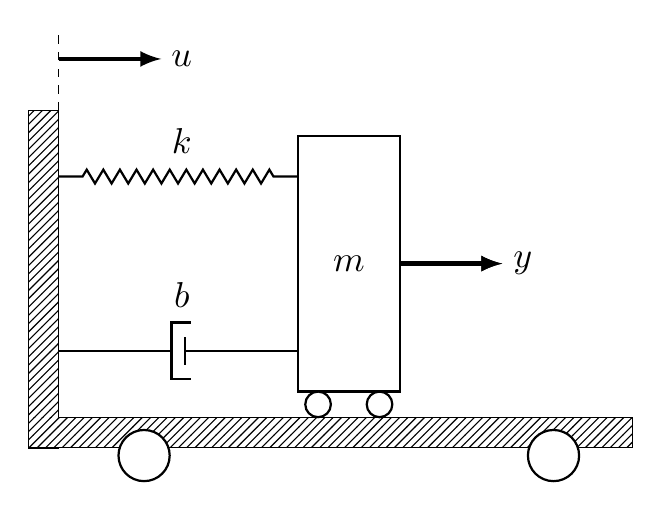
\begin{tikzpicture}[scale=1.3, every node/.style={scale=1.3}]
\tikzstyle{spring}=[thick,decorate,decoration={zigzag,pre length=0.3cm,post length=0.3cm,segment length=6}]
\tikzstyle{damper}=[thick,decoration={markings,  
  mark connection node=dmp,
  mark=at position 0.5 with 
  {
    \node (dmp) [thick,inner sep=0pt,transform shape,rotate=-90,minimum width=15pt,minimum height=3pt,draw=none] {};
    \draw [thick] ($(dmp.north east)+(2pt,0)$) -- (dmp.south east) -- (dmp.south west) -- ($(dmp.north west)+(2pt,0)$);
    \draw [thick] ($(dmp.north)+(0,-5pt)$) -- ($(dmp.north)+(0,5pt)$);
  }
}, decorate]
\tikzstyle{ground}=[fill,pattern=north east lines,draw=none,minimum width=0.75cm,minimum height=0.3cm,inner sep=0pt,outer sep=0pt]

\node [draw, outer sep=0pt, thick] (M) [minimum width=1cm, minimum height=2.5cm] {$m$};

\node (ground) [ground,anchor=north,yshift=-0.25cm,minimum width=5.6cm,xshift=-0.03cm] at (M.south) {};
\draw (ground.north east) -- (ground.north west);
\draw (ground.south east) -- (ground.south west);
\draw (ground.north east) -- (ground.south east);

%\node (ground) [anchor=north,yshift=-0.25cm,minimum width=5.6cm,xshift=-0.03cm] at (M.south) {};

\node (fill) [ground,xshift=-0.15cm,minimum height = 0.3cm, minimum width = 0.3cm] at (ground.west) {};
\draw (fill.north west) -- (fill.south west);
\draw (fill.south west) -- (fill.south east);

\draw [thick, fill=white] (M.south west) ++ (0.2cm,-0.125cm) circle (0.125cm)  (M.south east) ++ (-0.2cm,-0.125cm) circle (0.125cm);
\draw [thick, fill=white!100] (M.south west) ++ (2.5cm,-0.625cm) circle (0.25cm)  (M.south east) ++ (-2.5cm,-0.625cm) circle (0.25cm);
\node (wall) [ground, rotate=-90, minimum width=3cm,anchor=south east] at (fill.north west) {};
\draw (wall.north east) -- (wall.north west);
\draw (wall.north west) -- (wall.south west);
\draw (wall.south west) -- (wall.south east);

%\node (wall) [rotate=-90, minimum width=3cm,yshift=-3cm] {};

%\draw[pattern=north east lines ] (wall.south west)|-(ground.south east)|-(wall.north east)|- cycle;

\node (y) at (M.east) [xshift = 1.2cm] {$y$};

\draw [spring] (wall.170) -- ($(M.north west)!(wall.170)!(M.south west)$);
\draw [damper] (wall.10) -- ($(M.north west)!(wall.10)!(M.south west)$);

\draw [-latex,ultra thick] (M.east) ++ (0cm,0cm) -- +(1cm,0cm);
\node (b) at (wall.10) [xshift = 1.2cm,yshift=0.55cm] {$b$};
\node (k) at (wall.170) [xshift = 1.2cm,yshift=0.35cm] {$k$};

\draw [-latex,ultra thick] (M.east) ++ (0cm,0cm) -- +(1cm,0cm);
\draw [-latex,ultra thick] (wall.north west) ++ (0cm, 0.5cm) -- +(1cm,0cm);
\draw [dashed] (wall.north west) ++ (0cm, 0cm) -- +(0cm,0.8cm);
\node (u) at (wall.north west) [xshift = 1.2cm, yshift = 0.5cm] {$u$};
\end{tikzpicture}
\captionof{figure}{Block diagram of a simple mechanical system, analagous to a mass on a cart. Represented mathematically by Equation \ref{eq:3.1mechsys}}
  \label{fig:3.1mechsys}
\end{center}
\noindent
\begin{homeworkSection}{(a)}
Determine the transfer function $G(s) = \sfrac{Y(s)}{U(s)}$.

\sectionAnswer{
It is not stated, but an assumption will be made that all initial conditions are zero. Taking the Laplace transform of the equation modelling the system ($\mathcal{L}$[Equation \ref{eq:3.1mechsys}]) yields Equation \ref{eq:3.1mechsyslap}.

\begin{equation}\label{eq:3.1mechsyslap}
\begin{split}
ms^2 Y(s) + b s Y(s) + ks &= bs U(s) + kU(s) \\
Y(s) [ms^2 + bs+k] &= U(s)[bs+k]\\
G(s) = \frac{Y(s)}{U(s)} &= \frac{bs+k}{ms^2 + bs+k}
\end{split}
\end{equation}

}



\end{homeworkSection}


\begin{homeworkSection}{(b)}

Use the transfer function obtained in 3(a) to obtain a state-space representation of the system.

\sectionAnswer{
The transfer function for the system was obtained in Equation \ref{eq:3.1mechsyslap}. Comparing Equation \ref{eq:3.1mechsyslap} to the transfer function standard form (Equation \ref{eq:1.1estandard} but for $n=m$) it can be observed that:
\begin{equation}
a_n = \sfrac{k}{m} \text{ and }a_{n-1} = \sfrac{b}{m}
\end{equation}

With this small amount of knowledge it is possible to obtain part of the controllable Canonical form, as in Equation \ref{eq:contcan}.
\begin{equation*}
\text{Modified standard form: }
\begin{bmatrix}
   \dot{x_1}(t) \\ \dot{x_n}(t)
\end{bmatrix} =
\begin{bmatrix}
   0 & 1 \\ 
   -a_n & -a_{n-1}
\end{bmatrix}
\begin{bmatrix}
   {x_1(t)} \\ {x_n(t)}
\end{bmatrix} +
\begin{bmatrix}
   {0} \\ {1}
\end{bmatrix} u(t)
\end{equation*}

\begin{equation}\label{eq:contcan}
\begin{bmatrix}
   \dot{x_1}(t) \\ \dot{x_2}(t)
\end{bmatrix}
=
\begin{bmatrix}
   0 & 1 \\ 
   -\sfrac{k}{m} & -\sfrac{b}{m}
\end{bmatrix}
\begin{bmatrix}
   {x_1(t)} \\ {x_2(t)}
\end{bmatrix}
+
\begin{bmatrix}
   {0} \\ {1}
\end{bmatrix}
u(t)
\end{equation}

\begin{equation*}
a_n = \sfrac{k}{m} \text{, }b_n = \sfrac{k}{m} \text{, } a_1 = \sfrac{b}{m}\text{, } b_1 =\sfrac{b}{m} \text{ and } b_0 = 0 \text{ ($\because$ G(s) is strictly proper)}
\end{equation*}
With this information in mind, it is possible to complete the controllable Canonical form.
\begin{equation*}
\text{Modified standard form: }
y(t) =
\begin{bmatrix}
   (b_n - a_n b_0) & (b_1-a_1 b_0)
\end{bmatrix}
\begin{bmatrix}
   {x_1(t)} \\ {x_n(t)}
\end{bmatrix} + b_0 u(t)
\end{equation*}

\begin{equation}\label{eq:contcan2}
y(t) =
\begin{bmatrix}
  \sfrac{k}{m} & \sfrac{b}{m}
\end{bmatrix}
\begin{bmatrix}
   {x_1(t)} \\ {x_n(t)}
\end{bmatrix}
\end{equation}

Taking Equations \ref{eq:contcan} and \ref{eq:contcan2} into consideration, \textbf{one} state-space representation of $G(s)$ is complete, in controllable Canonical form. There are an infinite number of these. Matrices $\mathbf{A}$ (system), $\mathbf{B}$ (control), $\mathbf{C}$ (output) and $\mathbf{D}$ (feedforward) are given below.

\begin{equation*}
\mathbf{A} = 
\begin{bmatrix}
   0 & 1 \\ 
   -\sfrac{k}{m} & -\sfrac{b}{m}
\end{bmatrix}
\text{, }
\mathbf{B} = 
\begin{bmatrix}
   {0} \\ {1}
\end{bmatrix}\text{, }
\mathbf{C} = 
\begin{bmatrix}
  \sfrac{k}{m} & \sfrac{b}{m}
\end{bmatrix}
\text{, }
\mathbf{D} = 0
\end{equation*}

}

\end{homeworkSection}
\end{homeworkProblem}

\begin{homeworkProblem}[Exercise \#\arabic{homeworkProblemCounter}]
Consider a system represented by the following differential equations:
\begin{equation*}
Ri_1(t) + L_1 \frac{di_1(t)}{dt}+v(t) = v_a(t)
\end{equation*}
\begin{equation*}
L_2 \frac{di_2(t)}{dt}+v(t) = v_b(t)
\end{equation*}
\begin{equation*}
i_1(t) + i_2(t) = C\frac{dv(t)}{dt}
\end{equation*}
In this system, $R$, $L_1$, $L_2$ and $C$ are given constants, and $v_a(t)$ and $v_b(t)$ are inputs. Let the state variables be defined as $x_1(t) = i_1(t)$, $x_2(t) = i_2(t)$, and $x_3(t) = v(t)$. Obtain a state-space representation of the system where the output is $y(t)=x_3(t)$. Notice the system has two inputs and one output. 
\sectionAnswer{
The equations given in the question can be rewritten as in the below equations.
\begin{equation*}
Rx_1(t) + L_1 \frac{dx_1(t)}{dt}+x_3(t) = v_a(t)
\end{equation*}
\begin{equation*}
L_2 \frac{dx_2(t)}{dt}+x_3(t) = v_b(t)
\end{equation*}
\begin{equation*}
x_1(t) + x_2(t) = C\frac{dx_3(t)}{dt}
\end{equation*}
In terms of the required states, the above equations can be rewritten as below.
\begin{equation*}
\frac{dx_1(t)}{dt} = \frac{1}{L_1}v_a(t)-\frac{R}{L_1}x_1(t) -\frac{1}{L_1}x_3(t)
\end{equation*}
\begin{equation*}
\frac{dx_2(t)}{dt} = \frac{1}{L_2}v_b(t)-\frac{1}{L_2}x_3(t)
\end{equation*}
\begin{equation*}
\frac{dx_3(t)}{dt} = \frac{1}{C}x_1(t) + \frac{1}{C}x_2(t)
\end{equation*}
From here, it is very easy to obtain \textbf{one} state-space representation of the system.

\begin{equation*}
\begin{bmatrix}
   \dot{x_1}(t) \\ \dot{x_2}(t) \\ \dot{x_3}(t)
\end{bmatrix} =
\begin{bmatrix}
   -\sfrac{R}{L_1} & 0 & -\sfrac{1}{L_1} \\ 
   0 & 0 & -\sfrac{1}{L_2} \\ 
      \sfrac{1}{C} & \sfrac{1}{C} & 0 
\end{bmatrix}
\begin{bmatrix}
   {x_1(t)} \\ {x_2(t)} \\ {x_3(t)}
\end{bmatrix} +
\begin{bmatrix}
   \sfrac{1}{L_1} & 0 \\ 
   0 & \sfrac{1}{L_2} \\ 
     0 & 0 
\end{bmatrix}
\begin{bmatrix}
   v_a \\  v_b
\end{bmatrix}
\end{equation*}

\begin{equation*}
y = 
\begin{bmatrix}
   0 &  0 & 1
\end{bmatrix}
\begin{bmatrix}
   x_1(t) \\ x_2(t) \\ x_3(t)
\end{bmatrix}
\end{equation*}


\begin{equation*}
\mathbf{A} = 
\begin{bmatrix}
   -\sfrac{R}{L_1} & 0 & -\sfrac{1}{L_1} \\ 
   0 & 0 & -\sfrac{1}{L_2} \\ 
      \sfrac{1}{C} & \sfrac{1}{C} & 0 
\end{bmatrix}
\text{, }
\mathbf{B} = 
\begin{bmatrix}
   \sfrac{1}{L_1} & 0 \\ 
   0 & \sfrac{1}{L_2} \\ 
     0 & 0 
\end{bmatrix}\text{, }
\mathbf{C} = 
\begin{bmatrix}
   0 &  0 & 1
\end{bmatrix}
\text{, }
\mathbf{D} = 0
\end{equation*}


}

\end{homeworkProblem}


\begin{homeworkProblem}[Exercise \#\arabic{homeworkProblemCounter}]

A system is described by:
\begin{equation*}
\frac{d\mathbf{x}}{dt}=
\begin{bmatrix}
   2 & -1\\
   3 & -5
\end{bmatrix}\mathbf{x}+
\begin{bmatrix}
1 \\ 2 
\end{bmatrix}
u
\end{equation*}
\begin{equation*}
y=
\begin{bmatrix}
   1 & -1
\end{bmatrix}\mathbf{x}
\end{equation*}
\noindent
Determine the transfer function $G(s) = \sfrac{Y(s)}{U(s)}$.
\sectionAnswer{
It is possible to represent the matrix components of the state-space representation individually to simplify things.

\begin{equation}\label{eq:3.3abcd}
\mathbf{A} = 
\begin{bmatrix}
   2 & -1\\
   3 & -5
\end{bmatrix}
\text{, }
\mathbf{B} = 
\begin{bmatrix}
1 \\ 2 
\end{bmatrix}
\text{, }
\mathbf{C} = 
\begin{bmatrix}
   1 & -1
\end{bmatrix}
\text{, }
\mathbf{D} = 0
\end{equation}

The transfer function of a system can be represented in terms of these matrices,  $\mathbf{A}$, $\mathbf{B}$, $\mathbf{C}$ and $\mathbf{D}$.
\begin{equation}\label{eq:3.3transfuncabcd}
G(s) = \mathbf{C}(s\mathbf{I} - \mathbf{A})^{-1}\mathbf{B}+\mathbf{D}
\end{equation}
}
\sectionAnswer{
Using the values of  $\mathbf{A}$, $\mathbf{B}$, $\mathbf{C}$ and $\mathbf{D}$ obtained in Equation \ref{eq:3.3abcd} and substituting them into Equation \ref{eq:3.3transfuncabcd}, it is possible to obtain a system representation as in Equation \ref{eq:3.3ss2tf}.

\begin{subequations}
\begin{align}\label{eq:3.3ss2tf}
%%%%%%%%
G(s) &= \begin{bmatrix}
   1 & -1
\end{bmatrix}
\left(s
\begin{bmatrix}
   1 & 0 \\ 0 & 1
\end{bmatrix}
-
\begin{bmatrix}
   2 & -1\\
   3 & -5
\end{bmatrix}\right)^{-1}
\begin{bmatrix}
1 \\ 2 
\end{bmatrix}
+\begin{bmatrix}
0
\end{bmatrix}
\\
%%%%%%%%
&=  \begin{bmatrix}
   1 & -1
\end{bmatrix}
\begin{bmatrix}
  s-2 & 1\\
   -3 & s+5
\end{bmatrix}^{-1}
\begin{bmatrix}
1 \\ 2 
\end{bmatrix}\\
%%%%%%%
 &= \begin{bmatrix}
   1 & -1
\end{bmatrix}\left(
\frac{1}{(s-2)(s+5)+3}
\begin{bmatrix}
  s+5 & -1\\
   3 & s-2
\end{bmatrix}\right)
\begin{bmatrix}
1 \\ 2 
\end{bmatrix}
%%%%%%%
\\
 &= \begin{bmatrix}
   1 & -1
\end{bmatrix}
\frac{1}{(s-2)(s+5)+3}
\begin{bmatrix}
  s+5 & -1\\
   3 & s-2
\end{bmatrix}
\begin{bmatrix}
1 \\ 2 
\end{bmatrix}
%%%%%%%
\\
 &= \begin{bmatrix}
   1 & -1
\end{bmatrix}
\frac{1}{(s-2)(s+5)+3}
\begin{bmatrix}
  (s+5)+(2)(-1)\\
   3+2(s-2)
\end{bmatrix}
%%%%%%%
\\
 &= \frac{1}{(s-2)(s+5)+3}
\begin{bmatrix}
1 &-1
\end{bmatrix}
\begin{bmatrix}
  s+3\\
   2s-1
\end{bmatrix}\\
%%%%%%%%
 &= \frac{1}{(s-2)(s+5)+3}
\begin{bmatrix}
4-s
\end{bmatrix}\\
%%%%%%%%
 &= \frac{-s+4}{s^2 +3s -7}
\end{align}
\end{subequations}
}


\end{homeworkProblem}



\begin{homeworkProblem}[Exercise \#\arabic{homeworkProblemCounter}]
A system has the following transfer function representation:
\begin{equation*}
Q(s) = \frac{s^2 + 2s}{s^2(s^2+3s+4)}
\end{equation*}
Derive a state-space model for the system.
\sectionAnswer{

$Q(s)$ can be alternatively represented as in Equation \ref{eq:3.4qs}.

\begin{equation}\label{eq:3.4qs}
Q(s) = \frac{s^2 + 2s + 0}{s^4 + 3s^3 + 4s^2 + 0s +0}
\end{equation}

Compare this transfer function to the universal transfer function, which is reprinted in Equation \ref{eq:3.4tfst}.
\begin{equation}\label{eq:3.4tfst}
G(s) = \frac{Y(s)}{U(s)} = \frac{b_0 s^n + b_1 s^{n-1} + \cdots + b_{n-1}s+b_n}{s^n + a_1 s^{n-1} + \cdots + a_{n-1} s + a_n}
\end{equation}
}


\newsavebox{\codeboxk}% For storing code in a box
\begin{lrbox}{\codeboxk}
\begin{lstlisting}
>> A = [0 1 0 0; 0 0 1 0; 0 0 0 1; 0 0 -4 -3];
B = [0;0;0;1];
C = [0 2 1 0];
D = [0];
[n,d] = ss2tf(A,B,C,D)


n =

     0     0     1     2     0


d =

    1.0000    3.0000    4.0000         0         0
\end{lstlisting}
\end{lrbox}



\sectionAnswer{
The controllable Canonical state-space representation takes a form shown in Equation \ref{eq:3.4sscan}.
\begin{subequations}\label{eq:3.4sscan}
\begin{align}
\begin{bmatrix}
\dot{x_1}(t) \\ \dot{x_2}(t) \\ \vdots \\ \dot{x_{n-1}}(t) \\ \dot{x_n}(t)
\end{bmatrix}
&=
\begin{bmatrix}
0 & 1 & 0 &\cdots & 0 \\ 0 & 0 & 1 & \cdots & 0 \\ \vdots & \vdots & \vdots & & \vdots \\ 0 &0&0&\cdots&1 \\ -a_n & -a_{n-1} & -a_{n-2} & \cdots & -a_1
\end{bmatrix}
\begin{bmatrix}
{x_1}(t) \\ {x_2}(t) \\ \vdots \\ {x_{n-1}}(t) \\ {x_n}(t)
\end{bmatrix}+
\begin{bmatrix}
0\\ 0 \\ \vdots \\ 0 \\ 1
\end{bmatrix}u(t)\\
y(t) &=  
\begin{bmatrix}
b_n-a_nb_0 & b_{n-1}-a_{n-1}b_0 & \cdots & b_1-a_1b_0
\end{bmatrix}
\begin{bmatrix}
{x_1}(t) \\ {x_2}(t) \\ \vdots \\ {x_n}(t)
\end{bmatrix}+b_0u(t)
\end{align}
\end{subequations}

Comparing the transfer function given in Equation \ref{eq:3.4qs} with Equation \ref{eq:3.4tfst}, the coefficients of the various orders of $s$ can be observed and used to populated the matrices given in Equation \ref{eq:3.4sscan}. This leaves one state-space representation for $Q(s)$ as in Equation \ref{eq:3.4done}.

\begin{subequations}\label{eq:3.4done}
\begin{align}
\begin{bmatrix}
\dot{x_1}(t) \\ \dot{x_2}(t) \\ \dot{x_{3}}(t) \\ \dot{x_4}(t)
\end{bmatrix}
&=
\begin{bmatrix}
0 & 1 & 0 & 0 \\ 0 & 0 & 1& 0 \\ 0 & 0 & 0 & 1 \\ 0 & 0 & -4 & -3
\end{bmatrix}
\begin{bmatrix}
{x_1}(t) \\ {x_2}(t) \\ {x_3}(t) \\ {x_4}(t)
\end{bmatrix}+
\begin{bmatrix}
0\\ 0 \\ 0 \\ 1
\end{bmatrix}u(t)\\
y(t) &=  
\begin{bmatrix}
0 & 2 & 1& 0
\end{bmatrix}
\begin{bmatrix}
{x_1}(t) \\ {x_2}(t) \\ x_3(t) \\ {x_4}(t)
\end{bmatrix}
\end{align}
\end{subequations}

Just for fun, this can be tested using MATLAB.
%%%%%%%%%%%%%% CODE %%%%%%%%%%%%%%%
\begin{center}
\usebox{\codeboxk}%
\end{center}
%%%%%%%%%%%%%% CODE %%%%%%%%%%%%%%%
And, the coefficients of the polynomial given as \texttt{n} and \texttt{d} match the Equation of $Q(s)$ given in Equation \ref{eq:3.4qs}.
}
\end{homeworkProblem}



\begin{homeworkProblem}[Exercise \#\arabic{homeworkProblemCounter}]
Consider the system shown in Figure \ref{fig:3.5mechsys}. The equations modelling the system are shown below, as in Equations \ref{eq:3.5mechsys}.

\begin{equation}\label{eq:3.5mechsys}
\begin{split}
m_1 \frac{d^2 y_1(t)}{dt^2} + b\frac{dy_1(t)}{dt} + k[y_1(t)-y_2(t)]&=0\\
m_2 \frac{d^2y_2(t)}{dt^2} + k[y_2(t) -y_1(t)] &= u(t)
\end{split}
\end{equation}

\begin{center}
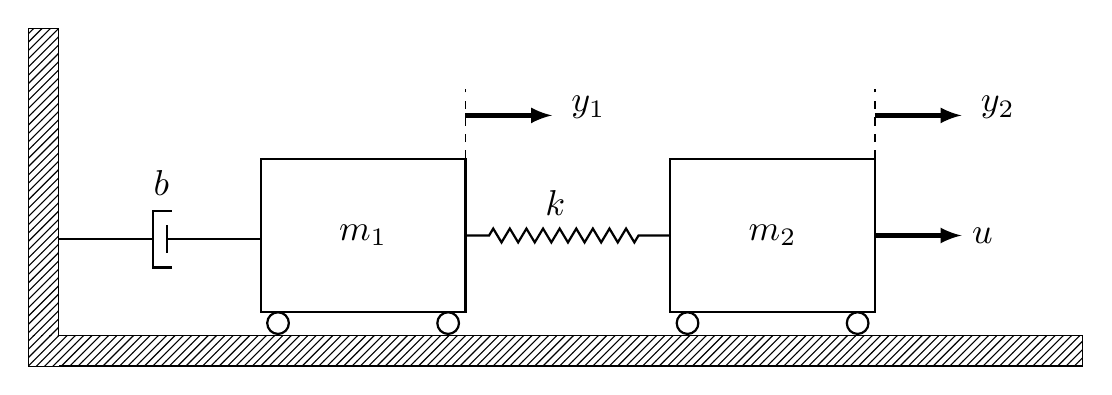
\begin{tikzpicture}[scale=1.1, every node/.style={scale=1.3}]
\tikzstyle{spring}=[thick,decorate,decoration={zigzag,pre length=0.3cm,post length=0.3cm,segment length=6}]
\tikzstyle{damper}=[thick,decoration={markings,  
  mark connection node=dmp,
  mark=at position 0.5 with 
  {
    \node (dmp) [thick,inner sep=0pt,transform shape,rotate=-90,minimum width=15pt,minimum height=3pt,draw=none] {};
    \draw [thick] ($(dmp.north east)+(2pt,0)$) -- (dmp.south east) -- (dmp.south west) -- ($(dmp.north west)+(2pt,0)$);
    \draw [thick] ($(dmp.north)+(0,-5pt)$) -- ($(dmp.north)+(0,5pt)$);
  }
}, decorate]
\tikzstyle{ground}=[fill,pattern=north east lines,draw=none,minimum width=0.75cm,minimum height=0.3cm,inner sep=0pt,outer sep=0pt]
%draw masses
\node [draw, outer sep=0pt, thick] (M) [minimum width=2cm, minimum height=1.5cm] {$m_1$};
\node [draw, outer sep=0pt, thick] (M2) [minimum width=2cm, minimum height=1.5cm, xshift = 4cm] {$m_2$};
% draw wheels on m1
\draw [thick, fill=white] (M2.south west) ++ (0.2cm,-0.125cm) circle (0.125cm)  (M2.south east) ++ (-0.2cm,-0.125cm) circle (0.125cm);
% draw the ground 
\node (ground) [ground,anchor=north,yshift=-0.225cm,minimum width=10cm,xshift=2.03cm] at (M.south) {};
\draw (ground.north east) -- (ground.north west);
\draw (ground.south east) -- (ground.south west);
\draw (ground.north east) -- (ground.south east);
% draw fill nodes
\node (fill) [ground,xshift=-0.15cm,minimum height = 0.3cm, minimum width = 0.3cm] at (ground.west) {};
\draw (fill.north west) -- (fill.south west);
\draw (fill.south west) -- (fill.south east);
%draw spring and wheels on m2
\draw [spring] (M.east) -- (M2.west);
\draw [thick, fill=white] (M.south west) ++ (0.2cm,-0.125cm) circle (0.125cm)  (M.south east) ++ (-0.2cm,-0.125cm) circle (0.125cm);
% draw wall and give border
\node (wall) [ground, rotate=-90, minimum width=3cm,anchor=south east] at (fill.north west) {};
\draw (wall.north east) -- (wall.north west);
\draw (wall.north west) -- (wall.south west);
\draw (wall.south west) -- (wall.south east);
% draw damper 
\draw [damper] (wall.15) -- ($(M.north west)!(wall.15)!(M.south west)$);
% damper and spring labels
\node (b) at (wall.15) [xshift = 1cm,yshift=0.55cm] {$b$};
\node (k) at (wall.15) [xshift = 4.85cm,yshift=0.35cm] {$k$};
%arrows and labels for inputs/outputs
\draw [-latex,ultra thick] (M2.east) ++ (0cm,0cm) -- +(1cm,0cm);
\draw [-latex,ultra thick] (M.north east) ++ (0cm, 0.5cm) -- +(1cm,0cm);
\draw [dashed] (M.north east) ++ (0cm, 0cm) -- +(0cm,0.8cm);
\node (y1) at (M.north east) [xshift = 1.2cm, yshift = 0.5cm] {$y_1$};
\draw [-latex,ultra thick] (M2.north east) ++ (0cm, 0.5cm) -- +(1cm,0cm);
\draw [dashed] (M2.north east) ++ (0cm, 0cm) -- +(0cm,0.8cm);
\node (y1) at (M2.north east) [xshift = 1.2cm, yshift = 0.5cm] {$y_2$};
\node (y1) at (M2.east) [xshift = 1.05cm] {$u$};
\end{tikzpicture}
\captionof{figure}{Masses-damper-spring system for Exercise 7. Represented mathematically by Equation \ref{eq:3.5mechsys}}
  \label{fig:3.5mechsys}
\end{center}


\noindent
Obtain a state-space representation if the output variables are $y_1(t)$ and $y_2(t)$. Notice that the system has one input and two outputs. 
\sectionAnswer{
The state variables can be defined as in Equation \ref{eq:3.5statevars}. By rearranging Equations \ref{eq:3.5mechsys} for the derivatives and substituting in the state variables, the set of equations shown below (Equations \ref{eq:3.5step1}) can be obtained. 
\begin{equation}\label{eq:3.5statevars}
\begin{split}
x_1 &= y_1\\ 
x_2 &= \sfrac{dy_1}{dt}\\
x_3 &= y_2\\
x_4 &= \sfrac{dy_2}{dt}
\end{split}
\end{equation}

\begin{equation}\label{eq:3.5step1}
\begin{split}
\frac{dx_1}{dt}&=x_2\\
\frac{dx_2}{dt}&= -\frac{b}{m_1}\frac{dy_1}{dt}-\frac{k}{m_1} (y_1-y_2)\\
\frac{dx_3}{dt}&= x_4\\
\frac{dx_4}{dt}&=-\frac{k}{m_2}(y_2-y_1)+\frac{u}{m_2}
\end{split}
\end{equation}


It is possible to further simplify Equations \ref{eq:3.5step1}. The final form of these equations is shown in \ref{eq:3.5step2}. From \ref{eq:3.5step2} the equations can then be expressed in matrix form, as in \ref{eq:3.5done}.

\begin{equation}\label{eq:3.5step2}
\begin{split}
\frac{dx_1}{dt}&=x_2\\
\frac{dx_2}{dt}&= -\frac{k}{m_1}x_1 - \frac{b}{m_1}x_2 + \frac{k}{m_1}x_3\\
\frac{dx_3}{dt}&= x_4\\
\frac{dx_4}{dt}&=\frac{1}{m_2}u + \frac{k}{m_2}x_1 - \frac{k}{m_2} x_3 
\end{split}
\end{equation}
}
\sectionAnswer{
\begin{equation}\label{eq:3.5done}
\begin{bmatrix}
\dot{x_1}(t) \\ \dot{x_2}(t) \\ \dot{x_{3}}(t) \\ \dot{x_4}(t)
\end{bmatrix}
=
\begin{bmatrix}
0 & 1 & 0 & 0 \\ -\sfrac{k}{m_1} & -\sfrac{b}{m_1} & \sfrac{k}{m_1} & 0 \\ 0 & 0 & 0 & 1 \\ \sfrac{k}{m_2} & 0 & -\sfrac{k}{m_2} & 0
\end{bmatrix}
\begin{bmatrix}
{x_1}(t) \\ {x_2}(t) \\ {x_3}(t) \\ {x_4}(t)
\end{bmatrix}+
\begin{bmatrix}
0\\ 0 \\ 0 \\ \sfrac{1}{m_2}
\end{bmatrix}u(t)
\end{equation}

From Equations \ref{eq:3.5step1}, particularly paying attention to $x_1 = y_1$ and $x_3=y_2$, it is possible to now derive the output equation as in Equation \ref{eq:3.5outeq}

\begin{equation}\label{eq:3.5outeq}
\begin{bmatrix}
y_1 \\ y_2
\end{bmatrix}
=
\begin{bmatrix}
1 & 0 & 0 & 0\\ 0 & 0 & 1 & 0
\end{bmatrix}
\begin{bmatrix}
x_1 \\ x_2 \\ x_3 \\ x_4
\end{bmatrix}
\end{equation}

\begin{equation}\label{eq:3.5abcd}
\mathbf{A} = 
\begin{bmatrix}
0 & 1 & 0 & 0 \\ -\sfrac{k}{m_1} & -\sfrac{b}{m_1} & \sfrac{k}{m_1} & 0 \\ 0 & 0 & 0 & 1 \\ \sfrac{k}{m_2} & 0 & -\sfrac{k}{m_2} & 0
\end{bmatrix}
\text{, }
\mathbf{B} = 
\begin{bmatrix}
0\\ 0 \\ 0 \\ \sfrac{1}{m_2}
\end{bmatrix}
\text{, }
\mathbf{C} = 
\begin{bmatrix}
1 & 0 & 0 & 0\\ 0 & 0 & 1 & 0
\end{bmatrix}
\text{, }
\mathbf{D} = 0
\end{equation}
}


\end{homeworkProblem}

\section{Section 3 - Design in State-Space}
\begin{homeworkProblem}[Exercise \#\arabic{homeworkProblemCounter}]
The system shown in Figure \ref{fig:4.1blocksimple} has a transfer function $G(s)$ given as in Equation \ref{eq:4.1eq}.

\begin{equation}\label{eq:4.1eq}
G(s) = \frac{4}{(s+1)(s+2)^2}
\end{equation}
This SISO system has a state-space representation, as given below in Equation \ref{eq:4.1ssequations}.
\begin{equation}\label{eq:4.1ssequations}
\begin{split}
\frac{d\mathbf{x}(t)}{dt} = \mathbf{Ax}(t) + \mathbf{B}u(t)\\
y(t) = \mathbf{Cx}(t) + \mathbf{D}u(t)
\end{split}
\end{equation}

\begin{center}
\tikzstyle{block} = [draw, fill=blue!20, rectangle, 
    minimum height=3em, minimum width=6em]
\tikzstyle{sum} = [draw, fill=blue!20, circle, node distance=1cm]
\tikzstyle{input} = [coordinate]
\tikzstyle{output} = [coordinate]
\tikzstyle{pinstyle} = [pin edge={to-,thin,black}]
\tikzstyle{dummy} = [coordinate]

% The block diagram code is probably more verbose than necessary
\begin{tikzpicture}[auto, node distance=2cm,>=latex']
	    % We start by placing the blocks
	    \node [input, name=input] {};
	    \node [block, right of=input, node distance=3cm] (system) {$G(s)$};
	    % We draw an edge between the controller and system block to 
	    % calculate the coordinate u. We need it to place the measurement block. 
	    \node [output, right of=system, node distance=3cm] (output) {};
	    \draw [right] (output) node [name=yt] {$y(t)$}(output);
	    \node [dummy,right of=output] (yt) {};
	    % Once the nodes are placed, connecting them is easy. 
	    \draw [left] (input) node [name=rt] {$u(t)$};
	    \draw [draw,->] (input) -- (system);
	    \draw [->] (system) -- node [name=y] {}(output);
\end{tikzpicture}
\captionof{figure}{Simple system for Exercise 8}
  \label{fig:4.1blocksimple}
\end{center}

\newsavebox{\codeboxl}% For storing code in a box
\begin{lrbox}{\codeboxl}
\begin{lstlisting}
>> A = [0 1 0; 0 0 1; -4 -8 -5]; 
B = [0; 0; 1]; 
C = [4 0 0]; D = [0]; 
K = [36 30 6];
sysnoK = ss(A, B, C, D);
sysK = ss(A-B*K,B,C,D);
sysK_gain = ss(A-B*K,10*B,C,D);
step(sysnoK)
hold % assuming you have not already got a figure held
step(sysK)
step(sysK_gain)
\end{lstlisting}
\end{lrbox}

\newsavebox{\codeboxm}% For storing code in a box
\begin{lrbox}{\codeboxm}
\begin{lstlisting}
>> syms s;
limit(((4*s)/((s^3 + 11*s^2 + 38*s + 40)*s)),s,0,'right')
 
ans =
 
1/10

\end{lstlisting}
\end{lrbox}

\begin{homeworkSection}{(a)}

Find matrices $\mathbf{A}$, $\mathbf{B}$, $\mathbf{C}$, and $\mathbf{D}$. Construct the characteristic polynomial of $\mathbf{A}$. Verify that the eigenvalues of $\mathbf{A}$ are the poles of G(s). 
\sectionAnswer{
Using Equations \ref{eq:3.4sscan} it is possible to derive the Canonical state-space representation for the system defined by the transfer function, as in Equation \ref{eq:4.1eq}.

\begin{subequations}\label{eq:4.1done}
\begin{align}
\begin{bmatrix}
\dot{x_1}(t) \\ \dot{x_2}(t) \\ \dot{x_{3}}(t) 
\end{bmatrix}
&=
\begin{bmatrix}
0 & 1 & 0 \\ 0 & 0 & 1 \\  -4 & -8 & -5 
\end{bmatrix}
\begin{bmatrix}
{x_1}(t) \\ {x_2}(t) \\ {x_3}(t) 
\end{bmatrix}+
\begin{bmatrix}
0\\ 0 \\ 1
\end{bmatrix}u(t)\\
y(t) &=  
\begin{bmatrix}
4 & 0 & 0
\end{bmatrix}
\begin{bmatrix}
{x_1}(t) \\ {x_2}(t) \\ x_3(t) 
\end{bmatrix}
\end{align}
\end{subequations}

\begin{equation}\label{eq:4.1abcd}
\mathbf{A} = 
\begin{bmatrix}
0 & 1 & 0 \\ 0 & 0 & 1 \\  -4 & -8 & -5 
\end{bmatrix}
\text{, }
\mathbf{B} = 
\begin{bmatrix}
0\\ 0 \\ 1
\end{bmatrix}
\text{, }
\mathbf{C} = 
\begin{bmatrix}
4 & 0 & 0
\end{bmatrix}
\text{, }
\mathbf{D} = 0
\end{equation}

The characteristic polynomial of $\mathbf{A}$ is given by Equation \ref{eq:4.1char}.

\begin{equation}\label{eq:4.1char}
\Delta (s) = \text{det}(s\mathbf{I} - \mathbf{A}) = |s\mathbf{I} - \mathbf{A}| = 0
\end{equation}

This characteristic polynomial is given in Equation \ref{eq:4.1charpoly}.

\begin{equation}\label{eq:4.1charpoly}
\begin{split}
\Delta(s) &= \left| s 
\begin{bmatrix}
1 & 0 & 0 \\ 0 & 1 & 0 \\ 0 & 0 & 1
\end{bmatrix}-
\begin{bmatrix}
0 & 1 & 0 \\ 0 & 0 & 1 \\  -4 & -8 & -5 
\end{bmatrix}\right| = 0\\
& = \left|
\begin{matrix}
s & -1 & 0 \\ 0 & s & -1 \\ 4 & 8 & s+5
\end{matrix}\right| = 0\\
& = s \left[(s)(s+5) - (-1)(8)\right] - (-1)\left[-(-1)(4)\right] + (0)\left[(\dots)\right] = 0\\
& = 
s^3 + 5s^2 + 8s + 4 = 0 
\end{split}
\end{equation}

The Eigenvalues of matrix $\mathbf{A}$ will be given by the roots of the characteristic polynomial, $\Delta(s)$ given in Equation \ref{eq:4.1charpoly}. To verify that the poles of $G(s)$ (i.e. the roots of  $(s+1)(s+2)^2 = 0$) are the same as the Eigenvalues of $\mathbf{A}$, the two polynomials should be equal. This is shown in Equation \ref{eq:4.1same?}. No further work is needed here, clearly the roots of these two polynomials will be the same, because they \textit{\textbf{are the same}} polynomial. 

\begin{equation}\label{eq:4.1same?}
\begin{split}
(s+1)(s+2)^2 & \stackrel{?}{=} s^3 + 5s^2 + 8s + 4\\
(s+1)(s+2)^2 & \stackrel{?}{=} (s+1)(s^2+4x+4)\\
(s+1)(s+2)^2 & = (s+1)(s+2)^2
\end{split}
\end{equation}
}

\end{homeworkSection}
\begin{homeworkSection}{(b)}
Verify that the system is controllable.
\sectionAnswer{
The system's controllability is analysed through the controllability matrix, $\mathbf{M}_c$. When this matrix has full-rank, that is to say, $\text{det}(\mathbf{M}_c) \neq 0$, the system can be said to be controllable. 

}

\sectionAnswer{
The controllability matrix,  $\mathbf{M}_c$, is given by Equation \ref{eq:4.1mc}.

\begin{equation}\label{eq:4.1mc}
\mathbf{M}_c = 
\begin{bmatrix}
\mathbf{B} &  \mathbf{AB} & \mathbf{A}^2 \mathbf{B}
\end{bmatrix}
\end{equation}

So, some matrix calculations are needed to simplify the calculation of $\mathbf{M}_c$.

\begin{equation*}
\mathbf{AB} = \begin{bmatrix}
0 & 1 & 0 \\ 0 & 0 & 1 \\  -4 & -8 & -5 
\end{bmatrix}
\begin{bmatrix}
0\\ 0 \\ 1
\end{bmatrix}=\begin{bmatrix}
0 \\ 1 \\ -5
\end{bmatrix}
\end{equation*}

\begin{equation*}
\begin{split}
\mathbf{A}^2 \mathbf{B} = \mathbf{A}(\mathbf{AB}) &= 
\begin{bmatrix}
0 & 1 & 0 \\ 0 & 0 & 1 \\  -4 & -8 & -5 
\end{bmatrix}\left(
\begin{bmatrix}
0 & 1 & 0 \\ 0 & 0 & 1 \\  -4 & -8 & -5 
\end{bmatrix}
\begin{bmatrix}
0\\ 0 \\ 1
\end{bmatrix}\right)\\
& = 
\begin{bmatrix}
0 & 1 & 0 \\ 0 & 0 & 1 \\  -4 & -8 & -5 
\end{bmatrix}
\begin{bmatrix}
0 \\ 1 \\ -5
\end{bmatrix}\\
& = \begin{bmatrix}
1 \\ -5 \\ 17
\end{bmatrix}
\end{split}
\end{equation*}

Therefore, $\mathbf{M}_c$ becomes obtainable, as in Equation \ref{eq:4.1mcfinal}. Next, the determinant of $\mathbf{M}_c$ can be found, as in Equation \ref{eq:4.1mcdet}. From this result, the system is determined to be controllable.

\begin{equation}\label{eq:4.1mcfinal}
\mathbf{M}_c = \begin{bmatrix}
0 & 0 & 1 \\
0 & 1 & -5 \\
1 & -5 & 17 
\end{bmatrix}
\end{equation}

\begin{equation}\label{eq:4.1mcdet}
\text{det}(\mathbf{M}_c) = (1) \left| \begin{matrix}
0 & 1  \\
1 & -5 
\end{matrix}\right| = -1
\end{equation}

}
\end{homeworkSection}

\begin{homeworkSection}{(c)}
Calculate a state feedback vector $\mathbf{K}$ that will move the poles of the system to $s_1 = -2$, $s_2 = -4$ and $s_3 = -5$. Calculate the amplification factor for the input pre-scaler. 

\sectionAnswer{
Introducing state feedback into the system will modify Equation \ref{eq:4.1ssequations} to become Equation \ref{eq:4.1mod}, where $\mathbf{K} = \begin{bmatrix}k_1 & k_2 & k_3\end{bmatrix}$.
\begin{equation}\label{eq:4.1mod}
\begin{split}
\frac{d\mathbf{x}(t)}{dt} &= \mathbf{Ax}(t) + \mathbf{B}\left[ u(t) - \mathbf{Kx}(t)\right]\\
& = (\mathbf{A} -\mathbf{BK}) \mathbf{x}(t) + \mathbf{B}u(t)
\end{split}
\end{equation}

The poles, $s_1$, $s_2$ and $s_3$ will now be the Eigenvalues of $\mathbf{A} - \mathbf{BK}$. Hence, the characteristic equation given by Equation \ref{eq:4.1charpoly} becomes as in Equation \ref{eq:4.1charpolymod}.

\begin{equation}\label{eq:4.1charpolymod}
\Delta_K(s) = \text{det}\left[s \mathbf{I}-(\mathbf{A} - \mathbf{BK} ) \right]= \left| s\mathbf{I} - \mathbf{A} + \mathbf{BK}\right| = 0 
\end{equation}

Working this through numerically,
}

\sectionAnswer{
\begin{equation*}
\begin{split}
\Delta_K(s) &= \left| s \begin{bmatrix}
1 & 0 & 0\\ 0 & 1 & 0 \\ 0 & 0 & 1
\end{bmatrix}
-
\begin{bmatrix}
0 & 1 & 0 \\ 0 & 0 & 1 \\  -4 & -8 & -5 
\end{bmatrix}+
\begin{bmatrix}
0\\ 0 \\ 1
\end{bmatrix}
\begin{bmatrix}
k_1 & k_2 & k_3
\end{bmatrix}\right| \\
&= \left| \begin{bmatrix}
s & -1 & 0 \\
0 & s & -1 \\
4 & 8 & s+5 
\end{bmatrix}+
\begin{bmatrix}
0 & 0 & 0 \\ 
0 & 0 & 0 \\
k_1 & k_2 & k_3
\end{bmatrix}\right| \\
&= \left| \begin{matrix}
s & -1 & 0 \\
0 & s & -1 \\
k_1 + 4 & k_2 + 8 & k_3 + s+5 
\end{matrix}
\right| \\
& = s [s(k_3 + s +5) + (k_2+8)] + (k_1+4)\\
& = s^3 + 5s^2 + k_3s^2 + 8s + k_2s + 4 + k_1\\
& = s^3 + s^2 (5+k_3) +s(8 +k_2) + 4 + k_1
\end{split}
\end{equation*}

Note that the poles can be represented as a factorised product, $(s_1 + 2)(s_2 + 4)(s_3 + 5)=0$. Therefore, in order to place the poles at these places, an equality is given as in Equation \ref{eq:4.1equalitygiven}.

\begin{equation}\label{eq:4.1equalitygiven}
\begin{split}
s^3 + s^2 (5+k_3) + s(8 +k_2) + 4 + k_1 &= (s_1 + 2)(s_2 + 4)(s_3 + 5)\\
s^3 + s^2 (5+k_3) + s(8 +k_2) + 4 + k_1 &= s^3 + 11s + 38s + 40
\end{split}
\end{equation}

Comparing coefficients, as in Equation \ref{eq:4.1coeff}, it is possible to obtains solutions for $k_1$, $k_2$ and $k_3$.
\begin{subequations}\label{eq:4.1coeff}
\begin{align}
5+k_3 &= 11\\
\Aboxed{\therefore k_3 & = 6}\\
8+k_2 & = 38\\
\Aboxed{\therefore k_2 &= 30}\\
4+k_1 & = 40\\
\Aboxed{\therefore k_1 &= 36}
\end{align}
\end{subequations}

With this knowledge, it is now possible to populate the state feedback gain matrix, $\mathbf{K}$ with its respective values.

\begin{equation*}
\mathbf{K} = \begin{bmatrix}
36 & 30 & 6
\end{bmatrix}
\end{equation*}

There are now essentially, two systems. One system is defined by $\mathbf{A}$, $\mathbf{B}$, $\mathbf{C}$, and $\mathbf{D}$ and another is defined by $\mathbf{A}^*$, $\mathbf{B}$, $\mathbf{C}$, and $\mathbf{D}$, where $\mathbf{A}^* = \mathbf{A}-\mathbf{BK}$. $\mathbf{A}^*$ is calculated in Equation \ref{eq:4.1anew}.

\begin{equation}\label{eq:4.1anew}
\mathbf{A}^* = \begin{bmatrix}
0 & 1 &0\\ 0 & 0 & 1 \\ -40 & -38 & -11
\end{bmatrix}
\end{equation}

With this new matrix in mind, it is possible to obtain the transfer function of this new state-space represented system. The transfer function of a system can be represented in terms of these matrices, $\mathbf{A^*}$, $\mathbf{B}$, $\mathbf{C}$, and $\mathbf{D}$, as in Equation \ref{eq:3.3transfuncabcd}. Noticing of course, that for this example, $\mathbf{A}$ of Equation  \ref{eq:3.3transfuncabcd} is substituted as $\mathbf{A^*}$, as in Equation \ref{eq:4.1anew}.
}

\sectionAnswer{

Representing $\mathbf{A^*}$, $\mathbf{B}$, $\mathbf{C}$, and $\mathbf{D}$ as a transfer function, will provide Equation \ref{eq:4.1ss2tfnew}.

\begin{equation}\label{eq:4.1ss2tfnew}
G^*(s) = \frac{4}{s^3 + 11s^2 + 38s + 40}
\end{equation}

It is now possible to apply the final value theorem (as in Equation \ref{eq:4.1fvt}) to $G^*(s)$. For a step input, the final value of $G^*(s)$ can be shown to be 0.1. 

\begin{equation}\label{eq:4.1fvt}
\lim_{t \to \infty} g^*(t) = \lim_{s \to 0} s G^*(s)
\end{equation}

Assuming the input to $G^*(s)$ is a step input i.e. $U(s) = \sfrac{1}{s}$, yields:

\begin{equation*}
G^*(s) = \frac{4}{(s^3 + 11s^2 + 38s + 40)(s)}
\end{equation*}

Applying the final value theorem: 

\begin{equation*}
\begin{split}
\lim_{s \to 0} s G^*(s) &= \lim_{s \to 0}\frac{4(s)}{(s^3 + 11s^2 + 38s + 40)(s)}\\
&= \lim_{s \to 0}\frac{4}{(s^3 + 11s^2 + 38s + 40)}\\
&= \frac{4}{((0)^3 + 11(0)^2 + 38(0) + 40)}\\
&=\frac{4}{40}\\
&= 0.1
\end{split}
\end{equation*}

This is verifiable with MATLAB. 

%%%%%%%%%%%%%% CODE %%%%%%%%%%%%%%%
\begin{center}
\usebox{\codeboxm}%
\end{center}
%%%%%%%%%%%%%% CODE %%%%%%%%%%%%%%%

Clearly, a final value of 0.1 is not what is required from the system. Therefore, an amplification factor is necessary. This amplification factor is 10. Let $G^*(s)$ now be the SISO transfer function for the system with state feedback, but also including an amplification factor. It can now be represented in state space.

\begin{equation*}
\mathbf{A^*} = 
\begin{bmatrix}
0 & 1 &0\\ 0 & 0 & 1 \\ -40 & -38 & -11
\end{bmatrix}
\text{, }
\mathbf{B^*} = 
10 \begin{bmatrix}
0\\ 0 \\ 1
\end{bmatrix}
\text{, }
\mathbf{C} = 
\begin{bmatrix}
4 & 0 & 0
\end{bmatrix}
\text{, }
\mathbf{D} = 0
\end{equation*}

}


\end{homeworkSection}



\begin{homeworkSection}{(d)}
Use MATLAB to plot the superimposed graphs of the step responses before and after applying the state feedback $\mathbf{K}$.

\sectionAnswer{
\begin{center}
% This file was created by matlab2tikz.
%
%The latest updates can be retrieved from
%  http://www.mathworks.com/matlabcentral/fileexchange/22022-matlab2tikz-matlab2tikz
%where you can also make suggestions and rate matlab2tikz.
%
\definecolor{mycolor1}{rgb}{0.00000,0.44700,0.74100}%
\definecolor{mycolor2}{rgb}{0.85000,0.32500,0.09800}%
\definecolor{mycolor3}{rgb}{0.92900,0.69400,0.12500}%
%
\begin{tikzpicture}

\begin{axis}[%
width=4.396in,
height=3.357in,
at={(0.883in,0.481in)},
scale only axis,
separate axis lines,
every outer x axis line/.append style={white!40!black},
every x tick label/.append style={font=\color{white!40!black}},
legend style={legend cell align=left,align=left,draw=white!15!black},
every x tick/.append style={white!40!black},
xmin=0,
xmax=8,
every outer y axis line/.append style={white!40!black},
every y tick label/.append style={font=\color{white!40!black}},
every y tick/.append style={white!40!black},
ymin=0,
ymax=1.3,
axis background/.style={fill=white}
]
\addplot [color=mycolor1]
  table[row sep=crcr]{%
0	0\\
0.0460517018598708	6.14765159815913e-05\\
0.0921034037197415	0.000464504703055503\\
0.138155105579612	0.00148109520024033\\
0.184206807439483	0.00331777722764986\\
0.230258509299354	0.00612568968649045\\
0.276310211159225	0.0100093730849615\\
0.322361913019095	0.0150344141550425\\
0.368413614878966	0.0212340782971078\\
0.414465316738837	0.0286150500320526\\
0.460517018598708	0.037162388271907\\
0.506568720458578	0.0468437912758891\\
0.552620422318449	0.0576132554921788\\
0.59867212417832	0.0694142029639605\\
0.644723826038191	0.0821821434824746\\
0.690775527898062	0.0958469300930165\\
0.736827229757932	0.110334659805988\\
0.782878931617803	0.12556926534797\\
0.828930633477674	0.141473838429935\\
0.874982335337545	0.157971720241598\\
0.921034037197416	0.174987390640165\\
0.967085739057286	0.192447183732437\\
1.01313744091716	0.210279854201056\\
1.05918914277703	0.228417015753806\\
1.1052408446369	0.246793470438794\\
1.15129254649677	0.265347445231951\\
1.19734424835664	0.28402075023425\\
1.24339595021651	0.302758870985268\\
1.28944765207638	0.321511005781252\\
1.33549935393625	0.340230057456516\\
1.38155105579612	0.358872587825928\\
1.42760275765599	0.377398741874845\\
1.47365445951586	0.395772147804583\\
1.51970616137574	0.413959798181382\\
1.56575786323561	0.431931916681706\\
1.61180956509548	0.449661814264635\\
1.65786126695535	0.46712573802259\\
1.70391296881522	0.484302715455173\\
1.74996467067509	0.501174396469154\\
1.79601637253496	0.517724895023024\\
1.84206807439483	0.533940632000508\\
1.8881197762547	0.549810180607888\\
1.93417147811457	0.565324115339786\\
1.98022317997444	0.58047486534245\\
2.02627488183431	0.595256572818307\\
2.07232658369418	0.609664956957102\\
2.11837828555406	0.623697183743774\\
2.16442998741393	0.637351741878652\\
2.2104816892738	0.65062832494886\\
2.25653339113367	0.663527719908751\\
2.30258509299354	0.676051701859745\\
2.34863679485341	0.688202935064306\\
2.39468849671328	0.69998488008344\\
2.44074019857315	0.711401706890517\\
2.48679190043302	0.722458213785376\\
2.53284360229289	0.7331597519103\\
2.57889530415276	0.743512155152737\\
2.62494700601263	0.753521675207694\\
2.6709987078725	0.763194921564842\\
2.71705040973238	0.772538806180909\\
2.76310211159225	0.781560492596343\\
2.80915381345212	0.790267349256013\\
2.85520551531199	0.798666906796477\\
2.90125721717186	0.806766819066703\\
2.94730891903173	0.814574827654804\\
2.9933606208916	0.822098729699982\\
3.03941232275147	0.829346348776377\\
3.08546402461134	0.836325508643533\\
3.13151572647121	0.843044009666677\\
3.17756742833108	0.849509607718741\\
3.22361913019095	0.855729995384946\\
3.26967083205082	0.861712785299712\\
3.3157225339107	0.867465495454563\\
3.36177423577057	0.872995536324514\\
3.40782593763044	0.878310199669035\\
3.45387763949031	0.883416648872164\\
3.49992934135018	0.88832191069449\\
3.54598104321005	0.893032868317684\\
3.59203274506992	0.897556255569847\\
3.63808444692979	0.901898652227277\\
3.68413614878966	0.906066480295274\\
3.73018785064953	0.91006600117723\\
3.7762395525094	0.913903313647665\\
3.82229125436927	0.917584352550846\\
3.86834295622914	0.921114888152353\\
3.91439465808902	0.924500526076366\\
3.96044635994889	0.927746707766504\\
4.00649806180876	0.930858711412839\\
4.05254976366863	0.93384165329225\\
4.0986014655285	0.936700489473425\\
4.14465316738837	0.939440017841851\\
4.19070486924824	0.942064880403782\\
4.23675657110811	0.944579565831647\\
4.28280827296798	0.946988412216567\\
4.32885997482785	0.949295609996681\\
4.37491167668772	0.951505205032727\\
4.42096337854759	0.953621101804956\\
4.46701508040746	0.955647066707845\\
4.51306678226734	0.957586731421292\\
4.55911848412721	0.959443596339063\\
4.60517018598708	0.961221034037159\\
4.65122188784695	0.962922292766505\\
4.69727358970682	0.964550499956034\\
4.74332529156669	0.966108665713681\\
4.78937699342656	0.967599686314227\\
4.83542869528643	0.969026347664141\\
4.8814803971463	0.970391328734772\\
4.92753209900617	0.971697204956281\\
4.97358380086604	0.972946451565667\\
5.01963550272591	0.974141446903143\\
5.06568720458579	0.975284475651917\\
5.11173890644566	0.97637773201716\\
5.15779060830553	0.977423322840633\\
5.2038423101654	0.978423270648028\\
5.24989401202527	0.979379516626634\\
5.29594571388514	0.980293923531446\\
5.34199741574501	0.981168278518274\\
5.38804911760488	0.982004295902795\\
5.43410081946475	0.982803619844891\\
5.48015252132462	0.983567826957894\\
5.52620422318449	0.984298428842684\\
5.57225592504436	0.984996874546818\\
5.61830762690423	0.985664552949104\\
5.66435932876411	0.986302795070238\\
5.71041103062398	0.986912876310286\\
5.75646273248385	0.98749601861396\\
5.80251443434372	0.98805339256475\\
5.84856613620359	0.988586119409112\\
5.89461783806346	0.98909527301199\\
5.94066953992333	0.989581881745046\\
5.9867212417832	0.99004693030902\\
6.03277294364307	0.990491361491723\\
6.07882464550294	0.990916077863194\\
6.12487634736281	0.991321943409592\\
6.17092804922268	0.991709785107402\\
6.21697975108255	0.992080394439592\\
6.26303145294242	0.992434528855317\\
6.3090831548023	0.992772913174806\\
6.35513485666217	0.993096240941041\\
6.40118655852204	0.99340517571986\\
6.44723826038191	0.993700352350055\\
6.49328996224178	0.993982378145074\\
6.53934166410165	0.994251834047875\\
6.58539336596152	0.994509275740477\\
6.63144506782139	0.994755234709722\\
6.67749676968126	0.994990219270739\\
6.72354847154113	0.995214715549558\\
6.769600173401	0.995429188426313\\
6.81565187526087	0.995634082440421\\
6.86170357712075	0.9958298226591\\
6.90775527898062	0.996016815510552\\
6.95380698084049	0.996195449583109\\
6.99985868270036	0.996366096391594\\
7.04591038456023	0.996529111112122\\
7.0919620864201	0.996684833286529\\
7.13801378827997	0.996833587497581\\
7.18406549013984	0.996975684016082\\
7.23011719199971	0.997111419420958\\
7.27616889385958	0.997241077193376\\
7.32222059571945	0.997364928285896\\
7.36827229757932	0.997483231667659\\
7.41432399943919	0.997596234846533\\
7.46037570129907	0.997704174369157\\
7.50642740315894	0.997807276299752\\
7.55247910501881	0.997905756678555\\
7.59853080687868	0.997999821960703\\
7.64458250873855	0.998089669436359\\
7.69063421059842	0.998175487632836\\
7.73668591245829	0.99825745669947\\
7.78273761431816	0.998335748775939\\
7.82878931617803	0.998410528344719\\
7.8748410180379	0.998481952568325\\
7.92089271989777	0.998550171611979\\
7.96694442175764	0.998615328952304\\
8.01299612361751	0.998677561672633\\
8.05904782547739	0.998737000745495\\
8.10509952733726	0.998793771302813\\
8.15115122919713	0.998847992894335\\
8.197202931057	0.998899779734799\\
8.24325463291687	0.998949240940302\\
8.28930633477674	0.99899648075434\\
8.33535803663661	0.999041598763953\\
8.38140973849648	0.999084690106401\\
8.42746144035635	0.999125845666775\\
8.47351314221622	0.999165152266934\\
8.51956484407609	0.999202692846133\\
8.56561654593596	0.999238546633708\\
8.61166824779584	0.999272789314164\\
8.65771994965571	0.999305493184975\\
8.70377165151558	0.999336727307439\\
8.74982335337545	0.999366557650858\\
8.79587505523532	0.999395047230366\\
8.84192675709519	0.999422256238651\\
8.88797845895506	0.999448242171855\\
8.93403016081493	0.999473059949901\\
8.9800818626748	0.999496762031489\\
9.02613356453467	0.999519398523994\\
9.07218526639454	0.99954101728849\\
9.11823696825441	0.999561664040115\\
9.16428867011428	0.999581382443979\\
9.21034037197416	0.999600214206807\\
9.25639207383403	0.999618199164514\\
9.3024437756939	0.999635375365884\\
9.34849547755377	0.999651779152525\\
9.39454717941364	0.999667445235261\\
9.44059888127351	0.999682406767134\\
9.48665058313338	0.999696695413138\\
9.53270228499325	0.999710341416859\\
9.57875398685312	0.999723373664133\\
9.62480568871299	0.999735819743873\\
9.67085739057286	0.999747706006176\\
9.71690909243273	0.99975905761784\\
9.7629607942926	0.999769898615401\\
9.80901249615247	0.9997802519558\\
9.85506419801234	0.999790139564787\\
9.90111589987222	0.999799582383165\\
9.94716760173209	0.999808600410962\\
9.99321930359196	0.999817212749631\\
10.0392710054518	0.999825437642359\\
10.0853227073117	0.999833292512578\\
10.1313744091716	0.999840794000751\\
10.1774261110314	0.999847957999504\\
10.2234778128913	0.999854799687199\\
10.2695295147512	0.999861333559992\\
10.3155812166111	0.999867573462461\\
10.3616329184709	0.999873532616859\\
10.4076846203308	0.999879223651059\\
10.4537363221907	0.999884658625244\\
10.4997880240505	0.999889849057406\\
10.5458397259104	0.999894805947694\\
10.5918914277703	0.999899539801675\\
10.6379431296301	0.999904060652553\\
10.68399483149	0.999908378082392\\
10.7300465333499	0.999912501242379\\
10.7760982352098	0.999916438872188\\
10.8221499370696	0.999920199318474\\
10.8682016389295	0.999923790552527\\
10.9142533407894	0.999927220187147\\
10.9603050426492	0.999930495492754\\
11.0063567445091	0.999933623412776\\
11.052408446369	0.999936610578346\\
11.0984601482289	0.999939463322343\\
11.1445118500887	0.999942187692796\\
11.1905635519486	0.99994478946569\\
11.2366152538085	0.999947274157198\\
11.2826669556683	0.999949647035361\\
11.3287186575282	0.999951913131243\\
11.3747703593881	0.999954077249591\\
11.420822061248	0.999956143979003\\
11.4668737631078	0.999958117701657\\
11.5129254649677	0.999960002602585\\
11.5589771668276	0.999961802678545\\
11.6050288686874	0.999963521746484\\
11.6510805705473	0.999965163451625\\
11.6971322724072	0.999966731275193\\
11.743183974267	0.999968228541788\\
11.7892356761269	0.99996965842643\\
11.8352873779868	0.999971023961289\\
11.8813390798467	0.999972328042106\\
11.9273907817065	0.999973573434334\\
11.9734424835664	0.999974762778996\\
12.0194941854263	0.999975898598284\\
12.0655458872861	0.999976983300902\\
12.111597589146	0.999978019187173\\
12.1576492910059	0.999979008453916\\
12.2037009928658	0.999979953199098\\
12.2497526947256	0.999980855426285\\
12.2958043965855	0.999981717048886\\
12.3418560984454	0.999982539894213\\
12.3879078003052	0.99998332570735\\
};
\addlegendentry{No SF};

\addplot [color=black, dotted, forget plot]
  table[row sep=crcr]{%
0	1\\
1	1\\
10	1\\
};
\addplot [color=mycolor2]
  table[row sep=crcr]{%
0	0\\
0.0184206807439514	3.9616870687323e-05\\
0.0368413614879028	0.000301393294607621\\
0.0552620422318543	0.000967565028592634\\
0.0736827229758057	0.00218212118954661\\
0.0921034037197571	0.00405603230526318\\
0.110524084463709	0.0066718757270818\\
0.12894476520766	0.010087921934115\\
0.147365445951611	0.0143417389092194\\
0.165786126695563	0.0194533660304648\\
0.184206807439514	0.0254281037407408\\
0.202627488183466	0.0322589605798621\\
0.221048168927417	0.0399287949404934\\
0.239468849671368	0.0484121850982455\\
0.25788953041532	0.0576770576282469\\
0.276310211159271	0.0676861012198697\\
0.294730891903223	0.078397990105903\\
0.313151572647174	0.0897684388031471\\
0.331572253391126	0.101751107591704\\
0.349992934135077	0.114298376116203\\
0.368413614879028	0.127362000652115\\
0.38683429562298	0.140893668924496\\
0.405254976366931	0.154845464877177\\
0.423675657110883	0.169170254451381\\
0.442096337854834	0.18382200222949\\
0.460517018598785	0.19875602771888\\
0.478937699342737	0.2139292090805\\
0.497358380086688	0.229300141236303\\
0.51577906083064	0.244829254508985\\
0.534199741574591	0.260478899247876\\
0.552620422318543	0.276213401268213\\
0.571041103062494	0.291999092370204\\
0.589461783806445	0.307804319702695\\
0.607882464550397	0.323599437287931\\
0.626303145294348	0.339356782623576\\
0.6447238260383	0.355050640920909\\
0.663144506782251	0.370657199219671\\
0.681565187526203	0.386154492336369\\
0.699985868270154	0.401522342350496\\
0.718406549014105	0.416742293108811\\
0.736827229758057	0.431797541028676\\
0.755247910502008	0.446672863304888\\
0.77366859124596	0.461354544468101\\
0.792089271989911	0.475830302104649\\
0.810509952733863	0.490089212425565\\
0.828930633477814	0.504121636264973\\
0.847351314221765	0.517919145993395\\
0.865771994965717	0.531474453748436\\
0.884192675709668	0.544781341312459\\
0.90261335645362	0.557834591903281\\
0.921034037197571	0.570629924088409\\
0.939454717941522	0.583163927985169\\
0.957875398685474	0.595434003867308\\
0.976296079429425	0.607438303262612\\
0.994716760173377	0.619175672595137\\
1.01313744091733	0.630645599399163\\
1.03155812166128	0.641848161109454\\
1.04997880240523	0.65278397641341\\
1.06839948314918	0.66345415913472\\
1.08682016389313	0.67386027460492\\
1.10524084463709	0.684004298468352\\
1.12366152538104	0.693888577857242\\
1.14208220612499	0.703515794866629\\
1.16050288686894	0.712888932253435\\
1.17892356761289	0.722011241279951\\
1.19734424835684	0.730886211619109\\
1.21576492910079	0.739517543237081\\
1.23418560984475	0.74790912016773\\
1.2526062905887	0.75606498609322\\
1.27102697133265	0.763989321645447\\
1.2894476520766	0.771686423343873\\
1.30786833282055	0.779160684086693\\
1.3262890135645	0.786416575113958\\
1.34470969430845	0.793458629363285\\
1.36313037505241	0.800291426141039\\
1.38155105579636	0.806919577034252\\
1.39997173654031	0.813347712991133\\
1.41839241728426	0.819580472500686\\
1.43681309802821	0.825622490804635\\
1.45523377877216	0.831478390077674\\
1.47365445951611	0.837152770514796\\
1.49207514026006	0.842650202267235\\
1.51049582100402	0.847975218171308\\
1.52891650174797	0.853132307217141\\
1.54733718249192	0.858125908706926\\
1.56575786323587	0.862960407054931\\
1.58417854397982	0.867640127184032\\
1.60259922472377	0.872169330475973\\
1.62101990546773	0.87655221123493\\
1.63944058621168	0.880792893626233\\
1.65786126695563	0.884895429054327\\
1.67628194769958	0.888863793946117\\
1.69470262844353	0.892701887907915\\
1.71312330918748	0.896413532226116\\
1.73154398993143	0.900002468683564\\
1.74996467067538	0.903472358665373\\
1.76838535141934	0.906826782529601\\
1.78680603216329	0.910069239219788\\
1.80522671290724	0.913203146097876\\
1.82364739365119	0.91623183897747\\
1.84206807439514	0.919158572338734\\
1.86048875513909	0.921986519707522\\
1.87890943588304	0.924718774182537\\
1.897330116627	0.927358349095468\\
1.91575079737095	0.929908178790111\\
1.9341714781149	0.932371119507525\\
1.95259215885885	0.934749950365193\\
1.9710128396028	0.937047374419081\\
1.98943352034675	0.939266019798317\\
2.0078542010907	0.941408440902999\\
2.02627488183466	0.943477119656396\\
2.04469556257861	0.945474466803478\\
2.06311624332256	0.947402823248377\\
2.08153692406651	0.949264461423978\\
2.09995760481046	0.951061586687406\\
2.11837828555441	0.952796338735713\\
2.13679896629836	0.954470793036536\\
2.15521964704232	0.956086962269002\\
2.17364032778627	0.957646797770526\\
2.19206100853022	0.959152190985596\\
2.21048168927417	0.960604974912985\\
2.22890237001812	0.96200692554817\\
2.24732305076207	0.963359763318066\\
2.26574373150602	0.964665154505485\\
2.28416441224998	0.965924712660976\\
2.30258509299393	0.967139999999992\\
2.32100577373788	0.968312528783534\\
2.33942645448183	0.969443762680649\\
2.35784713522578	0.970535118111366\\
2.37626781596973	0.971587965568823\\
2.39468849671368	0.972603630919511\\
2.41310917745764	0.973583396680734\\
2.43152985820159	0.974528503274489\\
2.44995053894554	0.975440150257144\\
2.46837121968949	0.97631949752438\\
2.48679190043344	0.977167666490976\\
2.50521258117739	0.977985741245147\\
2.52363326192134	0.978774769677183\\
2.5420539426653	0.97953576458226\\
2.56047462340925	0.980269704737371\\
2.5788953041532	0.980977535952347\\
2.59731598489715	0.981660172095061\\
2.6157366656411	0.982318496090916\\
2.63415734638505	0.982953360896788\\
2.652578027129	0.983565590449636\\
2.67099870787296	0.984155980590033\\
2.68941938861691	0.984725299960894\\
2.70784006936086	0.985274290881728\\
2.72626075010481	0.985803670198756\\
2.74468143084876	0.986314130111251\\
2.76310211159271	0.986806338974503\\
2.78152279233666	0.987280942079804\\
2.79994347308062	0.987738562411878\\
2.81836415382457	0.988179801384182\\
2.83678483456852	0.988605239552527\\
2.85520551531247	0.989015437307465\\
2.87362619605642	0.989410935545897\\
2.89204687680037	0.989792256322369\\
2.91046755754432	0.990159903480511\\
2.92888823828828	0.990514363265096\\
2.94730891903223	0.990856104915166\\
2.96572959977618	0.991185581238714\\
2.98415028052013	0.991503229169358\\
3.00257096126408	0.991809470305488\\
3.02099164200803	0.992104711432334\\
3.03941232275198	0.992389345027402\\
3.05783300349594	0.992663749749732\\
3.07625368423989	0.992928290913416\\
3.09467436498384	0.993183320945807\\
3.11309504572779	0.99342917983086\\
3.13151572647174	0.993666195538008\\
3.14993640721569	0.993894684436998\\
3.16835708795964	0.994114951699098\\
3.1867777687036	0.994327291685062\\
3.20519844944755	0.99453198832025\\
3.2236191301915	0.994729315457285\\
3.24203981093545	0.994919537226626\\
3.2604604916794	0.995102908375408\\
3.27888117242335	0.995279674594931\\
3.2973018531673	0.995450072837122\\
3.31572253391126	0.995614331620329\\
3.33414321465521	0.995772671324771\\
3.35256389539916	0.99592530447797\\
3.37098457614311	0.996072436030483\\
3.38940525688706	0.996214263622239\\
3.40782593763101	0.996350977839782\\
3.42624661837496	0.996482762464711\\
3.44466729911892	0.996609794713598\\
3.46308797986287	0.996732245469671\\
3.48150866060682	0.996850279506509\\
3.49992934135077	0.99696405570403\\
3.51835002209472	0.997073727257017\\
3.53677070283867	0.997179441876423\\
3.55519138358262	0.997281341983697\\
3.57361206432658	0.997379564898368\\
3.59203274507053	0.997474243019103\\
3.61045342581448	0.997565503998457\\
3.62887410655843	0.997653470911536\\
3.64729478730238	0.997738262418763\\
3.66571546804633	0.997819992922958\\
3.68413614879028	0.997898772720918\\
3.70255682953424	0.99797470814968\\
3.72097751027819	0.998047901727658\\
3.73939819102214	0.998118452290817\\
3.75781887176609	0.99818645512406\\
3.77623955251004	0.998252002087989\\
3.79466023325399	0.9983151817412\\
3.81308091399794	0.998376079458265\\
3.8315015947419	0.998434777543546\\
3.84992227548585	0.998491355340988\\
3.8683429562298	0.998545889340033\\
3.88676363697375	0.998598453277782\\
3.9051843177177	0.998649118237536\\
3.92360499846165	0.998697952743849\\
3.9420256792056	0.998745022854204\\
3.96044635994956	0.998790392247438\\
3.97886704069351	0.998834122309024\\
3.99728772143746	0.998876272213323\\
4.01570840218141	0.998916899002907\\
4.03412908292536	0.998956057665063\\
4.05254976366931	0.99899380120557\\
4.07097044441326	0.999030180719845\\
4.08939112515722	0.999065245461559\\
4.10781180590117	0.999099042908799\\
4.12623248664512	0.999131618827874\\
4.14465316738907	0.999163017334835\\
4.16307384813302	0.999193280954807\\
4.18149452887697	0.999222450679195\\
4.19991520962092	0.999250566020845\\
4.21833589036487	0.999277665067231\\
4.23675657110883	0.999303784531745\\
4.25517725185278	0.99932895980314\\
4.27359793259673	0.999353224993215\\
4.29201861334068	0.999376612982781\\
4.31043929408463	0.999399155465986\\
4.32885997482858	0.99942088299305\\
4.34728065557254	0.999441825011464\\
4.36570133631649	0.999462009905718\\
4.38412201706044	0.999481465035596\\
4.40254269780439	0.999500216773101\\
4.42096337854834	0.999518290538054\\
4.43938405929229	0.999535710832413\\
4.45780474003624	0.999552501273361\\
4.4762254207802	0.999568684625204\\
4.49464610152415	0.99958428283012\\
4.5130667822681	0.99959931703781\\
4.53148746301205	0.999613807634078\\
4.549908143756	0.99962777426838\\
4.56832882449995	0.999641235880387\\
4.5867495052439	0.999654210725593\\
4.60517018598785	0.999666716399999\\
4.62359086673181	0.999678769863908\\
4.64201154747576	0.999690387464863\\
4.66043222821971	0.999701584959765\\
4.67885290896366	0.999712377536187\\
4.69727358970761	0.999722779832925\\
4.71569427045156	0.999732805959805\\
4.73411495119552	0.999742469516783\\
4.75253563193947	0.999751783612348\\
4.77095631268342	0.99976076088127\\
20	0.9999999\\
};
\addlegendentry{SF, ampl. factor of 10};
\addplot [color=black, dotted, forget plot]
  table[row sep=crcr]{%
0	1\\
1	1\\
10	1\\
};
\addplot [color=mycolor3]
  table[row sep=crcr]{%
0	0\\
0.0184206807439514	3.9616870687323e-06\\
0.0368413614879028	3.01393294607621e-05\\
0.0552620422318543	9.67565028592633e-05\\
0.0736827229758057	0.000218212118954661\\
0.0921034037197571	0.000405603230526318\\
0.110524084463709	0.00066718757270818\\
0.12894476520766	0.0010087921934115\\
0.147365445951611	0.00143417389092194\\
0.165786126695563	0.00194533660304648\\
0.184206807439514	0.00254281037407408\\
0.202627488183466	0.00322589605798621\\
0.221048168927417	0.00399287949404934\\
0.239468849671368	0.00484121850982455\\
0.25788953041532	0.00576770576282469\\
0.276310211159271	0.00676861012198697\\
0.294730891903223	0.0078397990105903\\
0.313151572647174	0.00897684388031471\\
0.331572253391126	0.0101751107591704\\
0.349992934135077	0.0114298376116203\\
0.368413614879028	0.0127362000652115\\
0.38683429562298	0.0140893668924496\\
0.405254976366931	0.0154845464877177\\
0.423675657110883	0.0169170254451381\\
0.442096337854834	0.018382200222949\\
0.460517018598785	0.019875602771888\\
0.478937699342737	0.02139292090805\\
0.497358380086688	0.0229300141236303\\
0.51577906083064	0.0244829254508985\\
0.534199741574591	0.0260478899247876\\
0.552620422318543	0.0276213401268213\\
0.571041103062494	0.0291999092370204\\
0.589461783806445	0.0307804319702695\\
0.607882464550397	0.0323599437287931\\
0.626303145294348	0.0339356782623575\\
0.6447238260383	0.0355050640920909\\
0.663144506782251	0.0370657199219671\\
0.681565187526203	0.0386154492336368\\
0.699985868270154	0.0401522342350496\\
0.718406549014105	0.0416742293108811\\
0.736827229758057	0.0431797541028676\\
0.755247910502008	0.0446672863304888\\
0.77366859124596	0.04613545444681\\
0.792089271989911	0.0475830302104649\\
0.810509952733863	0.0490089212425565\\
0.828930633477814	0.0504121636264973\\
0.847351314221765	0.0517919145993395\\
0.865771994965717	0.0531474453748436\\
0.884192675709668	0.0544781341312459\\
0.90261335645362	0.0557834591903281\\
0.921034037197571	0.0570629924088409\\
0.939454717941522	0.0583163927985169\\
0.957875398685474	0.0595434003867308\\
0.976296079429425	0.0607438303262612\\
0.994716760173377	0.0619175672595137\\
1.01313744091733	0.0630645599399163\\
1.03155812166128	0.0641848161109455\\
1.04997880240523	0.065278397641341\\
1.06839948314918	0.066345415913472\\
1.08682016389313	0.067386027460492\\
1.10524084463709	0.0684004298468352\\
1.12366152538104	0.0693888577857242\\
1.14208220612499	0.0703515794866629\\
1.16050288686894	0.0712888932253435\\
1.17892356761289	0.0722011241279951\\
1.19734424835684	0.0730886211619109\\
1.21576492910079	0.0739517543237081\\
1.23418560984475	0.074790912016773\\
1.2526062905887	0.0756064986093221\\
1.27102697133265	0.0763989321645447\\
1.2894476520766	0.0771686423343873\\
1.30786833282055	0.0779160684086694\\
1.3262890135645	0.0786416575113958\\
1.34470969430845	0.0793458629363285\\
1.36313037505241	0.080029142614104\\
1.38155105579636	0.0806919577034252\\
1.39997173654031	0.0813347712991134\\
1.41839241728426	0.0819580472500686\\
1.43681309802821	0.0825622490804635\\
1.45523377877216	0.0831478390077674\\
1.47365445951611	0.0837152770514797\\
1.49207514026006	0.0842650202267235\\
1.51049582100402	0.0847975218171308\\
1.52891650174797	0.0853132307217141\\
1.54733718249192	0.0858125908706926\\
1.56575786323587	0.0862960407054931\\
1.58417854397982	0.0867640127184032\\
1.60259922472377	0.0872169330475973\\
1.62101990546773	0.087655221123493\\
1.63944058621168	0.0880792893626233\\
1.65786126695563	0.0884895429054327\\
1.67628194769958	0.0888863793946117\\
1.69470262844353	0.0892701887907915\\
1.71312330918748	0.0896413532226116\\
1.73154398993143	0.0900002468683564\\
1.74996467067538	0.0903472358665373\\
1.76838535141934	0.0906826782529601\\
1.78680603216329	0.0910069239219787\\
1.80522671290724	0.0913203146097875\\
1.82364739365119	0.0916231838977469\\
1.84206807439514	0.0919158572338733\\
1.86048875513909	0.0921986519707522\\
1.87890943588304	0.0924718774182537\\
1.897330116627	0.0927358349095468\\
1.91575079737095	0.0929908178790111\\
1.9341714781149	0.0932371119507525\\
1.95259215885885	0.0934749950365193\\
1.9710128396028	0.0937047374419081\\
1.98943352034675	0.0939266019798317\\
2.0078542010907	0.0941408440902999\\
2.02627488183466	0.0943477119656396\\
2.04469556257861	0.0945474466803478\\
2.06311624332256	0.0947402823248377\\
2.08153692406651	0.0949264461423978\\
2.09995760481046	0.0951061586687406\\
2.11837828555441	0.0952796338735712\\
2.13679896629836	0.0954470793036536\\
2.15521964704232	0.0956086962269002\\
2.17364032778627	0.0957646797770525\\
2.19206100853022	0.0959152190985595\\
2.21048168927417	0.0960604974912985\\
2.22890237001812	0.096200692554817\\
2.24732305076207	0.0963359763318066\\
2.26574373150602	0.0964665154505485\\
2.28416441224998	0.0965924712660976\\
2.30258509299393	0.0967139999999992\\
2.32100577373788	0.0968312528783534\\
2.33942645448183	0.0969443762680649\\
2.35784713522578	0.0970535118111366\\
2.37626781596973	0.0971587965568822\\
2.39468849671368	0.0972603630919511\\
2.41310917745764	0.0973583396680733\\
2.43152985820159	0.0974528503274489\\
2.44995053894554	0.0975440150257144\\
2.46837121968949	0.097631949752438\\
2.48679190043344	0.0977167666490976\\
2.50521258117739	0.0977985741245147\\
2.52363326192134	0.0978774769677182\\
2.5420539426653	0.097953576458226\\
2.56047462340925	0.0980269704737371\\
2.5788953041532	0.0980977535952347\\
2.59731598489715	0.0981660172095061\\
2.6157366656411	0.0982318496090916\\
2.63415734638505	0.0982953360896787\\
2.652578027129	0.0983565590449636\\
2.67099870787296	0.0984155980590033\\
2.68941938861691	0.0984725299960893\\
2.70784006936086	0.0985274290881728\\
2.72626075010481	0.0985803670198756\\
2.74468143084876	0.0986314130111251\\
2.76310211159271	0.0986806338974502\\
2.78152279233666	0.0987280942079803\\
2.79994347308062	0.0987738562411877\\
2.81836415382457	0.0988179801384182\\
2.83678483456852	0.0988605239552527\\
2.85520551531247	0.0989015437307465\\
2.87362619605642	0.0989410935545897\\
2.89204687680037	0.0989792256322369\\
2.91046755754432	0.0990159903480511\\
2.92888823828828	0.0990514363265095\\
2.94730891903223	0.0990856104915166\\
2.96572959977618	0.0991185581238714\\
2.98415028052013	0.0991503229169357\\
3.00257096126408	0.0991809470305488\\
3.02099164200803	0.0992104711432334\\
3.03941232275198	0.0992389345027402\\
3.05783300349594	0.0992663749749732\\
3.07625368423989	0.0992928290913415\\
3.09467436498384	0.0993183320945807\\
3.11309504572779	0.099342917983086\\
3.13151572647174	0.0993666195538007\\
3.14993640721569	0.0993894684436997\\
3.16835708795964	0.0994114951699098\\
3.1867777687036	0.0994327291685062\\
3.20519844944755	0.099453198832025\\
3.2236191301915	0.0994729315457285\\
3.24203981093545	0.0994919537226625\\
3.2604604916794	0.0995102908375407\\
3.27888117242335	0.0995279674594931\\
3.2973018531673	0.0995450072837122\\
3.31572253391126	0.0995614331620329\\
3.33414321465521	0.0995772671324771\\
3.35256389539916	0.099592530447797\\
3.37098457614311	0.0996072436030483\\
3.38940525688706	0.0996214263622239\\
3.40782593763101	0.0996350977839782\\
3.42624661837496	0.0996482762464711\\
3.44466729911892	0.0996609794713599\\
3.46308797986287	0.0996732245469671\\
3.48150866060682	0.0996850279506509\\
3.49992934135077	0.099696405570403\\
3.51835002209472	0.0997073727257018\\
3.53677070283867	0.0997179441876423\\
3.55519138358262	0.0997281341983697\\
3.57361206432658	0.0997379564898369\\
3.59203274507053	0.0997474243019103\\
3.61045342581448	0.0997565503998458\\
3.62887410655843	0.0997653470911536\\
3.64729478730238	0.0997738262418763\\
3.66571546804633	0.0997819992922958\\
3.68413614879028	0.0997898772720918\\
3.70255682953424	0.099797470814968\\
3.72097751027819	0.0998047901727658\\
3.73939819102214	0.0998118452290817\\
3.75781887176609	0.099818645512406\\
3.77623955251004	0.0998252002087989\\
3.79466023325399	0.0998315181741201\\
3.81308091399794	0.0998376079458266\\
3.8315015947419	0.0998434777543546\\
3.84992227548585	0.0998491355340988\\
3.8683429562298	0.0998545889340033\\
3.88676363697375	0.0998598453277782\\
3.9051843177177	0.0998649118237536\\
3.92360499846165	0.0998697952743849\\
3.9420256792056	0.0998745022854204\\
3.96044635994956	0.0998790392247438\\
3.97886704069351	0.0998834122309024\\
3.99728772143746	0.0998876272213323\\
4.01570840218141	0.0998916899002908\\
4.03412908292536	0.0998956057665064\\
4.05254976366931	0.099899380120557\\
4.07097044441326	0.0999030180719845\\
4.08939112515722	0.0999065245461559\\
4.10781180590117	0.09990990429088\\
4.12623248664512	0.0999131618827875\\
4.14465316738907	0.0999163017334835\\
4.16307384813302	0.0999193280954808\\
4.18149452887697	0.0999222450679196\\
4.19991520962092	0.0999250566020845\\
4.21833589036487	0.0999277665067231\\
4.23675657110883	0.0999303784531745\\
4.25517725185278	0.099932895980314\\
4.27359793259673	0.0999353224993215\\
4.29201861334068	0.0999376612982781\\
4.31043929408463	0.0999399155465986\\
4.32885997482858	0.099942088299305\\
4.34728065557254	0.0999441825011465\\
4.36570133631649	0.0999462009905718\\
4.38412201706044	0.0999481465035596\\
4.40254269780439	0.0999500216773101\\
4.42096337854834	0.0999518290538054\\
4.43938405929229	0.0999535710832414\\
4.45780474003624	0.0999552501273362\\
4.4762254207802	0.0999568684625204\\
4.49464610152415	0.099958428283012\\
4.5130667822681	0.0999599317037811\\
4.53148746301205	0.0999613807634079\\
4.549908143756	0.099962777426838\\
4.56832882449995	0.0999641235880387\\
4.5867495052439	0.0999654210725593\\
4.60517018598785	0.0999666716399999\\
4.62359086673181	0.0999678769863908\\
4.64201154747576	0.0999690387464863\\
4.66043222821971	0.0999701584959766\\
4.67885290896366	0.0999712377536188\\
4.69727358970761	0.0999722779832925\\
4.71569427045156	0.0999732805959806\\
4.73411495119552	0.0999742469516784\\
4.75253563193947	0.0999751783612349\\
4.77095631268342	0.0999760760881271\\
10 	0.099999\\
};
\addlegendentry{SF, no ampl. factor};

\addplot [color=black, dotted, forget plot]
  table[row sep=crcr]{%
0	0.1\\
1	0.1\\
10	0.1\\
};
\end{axis}

\begin{axis}[%
width=4.521in,
height=3.566in,
at={(0.758in,0.481in)},
scale only axis,
xmin=0,
xmax=1,
xtick={\empty},
xlabel={Time (s)},
ymin=0,
ymax=1,
ytick={\empty},
ylabel={Amplitude},
axis line style={draw=none},
ticks=none,
title style={font=\bfseries},
title={Step Response with and without State Feedback},
axis x line*=bottom,
axis y line*=left,
legend style={legend cell align=left,align=left,draw=white!15!black}
]
\end{axis}
\end{tikzpicture}%
\captionof{figure}{Step Response for $P(s)$ Plot with $k$ as Scalar}
  \label{fig:2.1}
\end{center}

%%%%%%%%%%%%%% CODE %%%%%%%%%%%%%%%
\begin{center}
\usebox{\codeboxl}%
\end{center}
%%%%%%%%%%%%%% CODE %%%%%%%%%%%%%%%
}


\end{homeworkSection}

\begin{homeworkSection}{(e)}
Verify that the system is observable.
\sectionAnswer{
The system will be observable if the observability matrix, $\mathbf{M}_O$ has full-rank. That is to say, $\text{det}(\mathbf{M_O}) \neq 0$. For this system, an observability matrix is derived as in Equation \ref{eq:4.1observmat}.

\begin{equation}\label{eq:4.1observmat}
\mathbf{M}_O = \begin{bmatrix}
\mathbf{C} \\
\mathbf{CA} \\
\mathbf{CA}^2
\end{bmatrix}
\end{equation}

}
\sectionAnswer{
So, some matrix calculations are needed to simplify the calculation of $\mathbf{M}_O$. 
\begin{equation*}
\begin{split}
\mathbf{CA} &= \begin{bmatrix}
4 & 0 & 0
\end{bmatrix}
\begin{bmatrix}
0 & 1 & 0 \\ 0 & 0 & 1 \\  -4 & -8 & -5 
\end{bmatrix}\\
& = \begin{bmatrix}
0 & 4 & 0 
\end{bmatrix}\\
\mathbf{CA}^2 &= (\mathbf{CA})\mathbf{A} = \begin{bmatrix}
0 & 4 & 0 
\end{bmatrix}
\begin{bmatrix}
0 & 1 & 0 \\ 0 & 0 & 1 \\  -4 & -8 & -5 
\end{bmatrix}\\
& = \begin{bmatrix}
0 & 0 & 4
\end{bmatrix}
\end{split}
\end{equation*}

Therefore, $\mathbf{M}_O$ becomes obtainable, as in Equation \ref{eq:4.1obsfin}. Next the determinant of $\mathbf{M}_O$ can be found, as in Equation \ref{eq:4.1obsdet}. From this result, the system is determined to be observable. 

\begin{equation}\label{eq:4.1obsfin}
\mathbf{M}_O = \begin{bmatrix}
4 & 0 & 0 \\
0 & 4 & 0 \\
0 & 0 & 4 
\end{bmatrix}
\end{equation}

\begin{equation}\label{eq:4.1obsdet}
\text{det}(\mathbf{M}_O) = (4) \left| \begin{matrix}
4 & 0  \\
0 & 4 
\end{matrix}\right| = 64
\end{equation}

}

\end{homeworkSection}
\begin{homeworkSection}{(f)}
Design an observer to track the states of the system. Place all the poles of this observer $-4$ rad/s. 
\sectionAnswer{
The system has already been determined to be observable. The observer error equation is shown in Equation \ref{eq:4.1erreq}, where $\mathbf{K}_e = \begin{bmatrix}k_{e1} \\ k_{e2}\\ k_{e3}\end{bmatrix}$.
\begin{equation}\label{eq:4.1erreq}
\frac{d\mathbf{e}(t)}{dt} = (\mathbf{A}- \mathbf{K}_e \mathbf{C}) \mathbf{e}(t)
\end{equation}

Much like the state feedback vector, the observer poles that are specified should be the Eigenvalues of $\mathbf{A} - \mathbf{K}_e \mathbf{C}$. The characteristic equation for the observer is shown in Equation \ref{eq:4.1obseq}.

\begin{equation}\label{eq:4.1obseq}
\Delta_{\mathbf{K}_e}(s)= \text{det}[s\mathbf{I} - (\mathbf{A}-\mathbf{K}_e\mathbf{C})] = |s\mathbf{I} - \mathbf{A} +\mathbf{K}_e \mathbf{C}| =0
\end{equation}
Substituting the required matrices into Equation \ref{eq:4.1obseq} provides the values for $k_{\text{1, 2, 3}}$.
\begin{equation*}
\begin{split}
\Delta_{\mathbf{K}_e}(s) &= \left|s\begin{bmatrix}1 & 0 & 0 \\ 0 & 1 & 0 \\ 0 & 0 & 1\end{bmatrix}-
\begin{bmatrix}0 & 1 & 0 \\ 0 & 0 &1\\-4 & -8 & -5\end{bmatrix}+
\begin{bmatrix}k_{e1} \\ k_{e2}\\ k_{e3}\end{bmatrix}
\begin{bmatrix}4 & 0 & 0\end{bmatrix}\right|\\
&= \left| \begin{bmatrix}s & -1 & 0 \\ 0 & s & -1\\ 4 & 8 & s+5\end{bmatrix}+
\begin{bmatrix}4k_{e1} & 0 &0 \\ 4k_{e2} & 0 & 0\\ 4k_{e3} & 0 & 0\end{bmatrix}\right|\\
& = \left| \begin{matrix} 4k_{e1}+s & -1 & 0 \\ 4k_{e2} & s & -1\\ 4k_{e3}+4 & 8 & s+5\end{matrix}\right|\\
& = s^3 + 5s^2 + 4k_{e1}s^2 + 8s + 20k_{e1}s + 4k_{e2}s + 32k_{e1} + 20k_{e2} + 4k_{e3} + 4\\
& = s^3 + s^2(5 + 4k_{e1}) + s(8+20k_{e1} + 4k_{e2})  + 32k_{e1} + 20k_{e2} + 4k_{e3} + 4
\end{split}
\end{equation*}
}
\sectionAnswer{
In order to have all of the poles at $-4$ rad/s, $s_{\text{1, 2, 3}} = -4$. With this in mind, coefficients can begin to be equated and solved for, as in Equations \ref{eq:4.1equalitygivenobs} and \ref{eq:4.1coeffobs}. 

\begin{equation}\label{eq:4.1equalitygivenobs}
\begin{split}
s^3 + s^2(5 + 4k_{e1}) + s(8+20k_{e1} + 4k_{e2})  + 32k_{e1} + 20k_{e2} + 4k_{e3} + 4 &= (s_1 + 4)(s_2 + 4)(s_3 + 4)\\
s^3 + s^2(5 + 4k_{e1}) + s(8+20k_{e1} + 4k_{e2})  + 32k_{e1} + 20k_{e2} + 4k_{e3} + 4 &= s^3 + 12s^2 + 48s + 64
\end{split}
\end{equation}
\begin{subequations}\label{eq:4.1coeffobs}
\begin{align}
5+4k_{e1} &= 12\\
\Aboxed{\therefore k_{e1} & = \sfrac{7}{4}}\\
8+20k_{e1} + 4k_{e2} & = 48\\
\Aboxed{\therefore k_{e2} &= 5}\\
4+ 32k_{e1} + 20k_{e2} + 4k_{e3} & = 64\\
\Aboxed{\therefore k_{e3} &= -24}
\end{align}
\end{subequations}

Therefore, the observer gain matrix is shown to be Equation \ref{eq:4.1obsgainmatrix}.

\begin{equation}\label{eq:4.1obsgainmatrix}
\mathbf{K}_e = \begin{bmatrix}\sfrac{7}{4} \\ 5 \\ -24\end{bmatrix}
\end{equation}


}



\end{homeworkSection}

\end{homeworkProblem}


\newsavebox{\codeboxo}% For storing code in a box
\begin{lrbox}{\codeboxo}
\begin{lstlisting}
>> r = [-2 -1+i -1-i];
poly(r)

ans =

     1     4     6     4
\end{lstlisting}
\end{lrbox}


\begin{homeworkProblem}[Exercise \#\arabic{homeworkProblemCounter}]
Consider a linear system of the form: 
\begin{equation*}
\begin{split}
\frac{d\mathbf{x}(t)}{dt} = \mathbf{Ax}(t) + \mathbf{B}u(t)\\
y(t) = \mathbf{Cx}(t) + \mathbf{D}u(t)
\end{split}
\end{equation*}
\noindent
Where,
\begin{equation}\label{eq:4.2start}
\mathbf{A} = \begin{bmatrix}0 & 1 & 0\\ 0 & 0 & 1\\ -4 & -1 & -2\end{bmatrix}\text{, }
\mathbf{B} = \begin{bmatrix}0 \\ 0\\ 1\end{bmatrix}\text{, }
\mathbf{C} = \begin{bmatrix}1 & 1 & 0\end{bmatrix}\text{ and }
\mathbf{D} = \begin{bmatrix}0\end{bmatrix}
\end{equation}
\begin{homeworkSection}{(a)}
Verify the system is controllable and observable. 
\sectionAnswer{
The controllability matrix,  $\mathbf{M}_c$, is given by Equation \ref{eq:4.1mc}.
So, some matrix calculations are needed to simplify the calculation of $\mathbf{M}_c$.
\begin{equation*}
\begin{split}
\mathbf{AB} &= \begin{bmatrix}0 & 1 & 0\\ 0 & 0 & 1\\ -4 & -1 & -2\end{bmatrix}
\begin{bmatrix}
0\\ 0 \\ 1
\end{bmatrix}=\begin{bmatrix}
0 \\ 1 \\ -2
\end{bmatrix}\\
\mathbf{A}^2 \mathbf{B} = \mathbf{A}(\mathbf{AB}) &= 
\begin{bmatrix}0 & 1 & 0\\ 0 & 0 & 1\\ -4 & -1 & -2\end{bmatrix}
\begin{bmatrix}
0 \\ 1 \\ -2
\end{bmatrix}\\
& = \begin{bmatrix}
1 \\ -2 \\ 3
\end{bmatrix}
\end{split}
\end{equation*}
Therefore, $\mathbf{M}_c$ becomes obtainable, as in Equation \ref{eq:4.2mcfinal}. Next, the determinant of $\mathbf{M}_c$ can be found, as in Equation \ref{eq:4.2mcdet}. From this result, the system is determined to be controllable.
\begin{equation}\label{eq:4.2mcfinal}
\mathbf{M}_c = \begin{bmatrix}
0 & 0 & 1 \\
0 & 1 & -2 \\
1 & -2 & 3
\end{bmatrix}
\end{equation}
\begin{equation}\label{eq:4.2mcdet}
\text{det}(\mathbf{M}_c) = (1) \left| \begin{matrix}
0 & 1  \\
1 & -2 
\end{matrix}\right| = -1
\end{equation}


The system will be observable if the observability matrix, $\mathbf{M}_O$ has full-rank. That is to say, $\text{det}(\mathbf{M_O}) \neq 0$. For this system, an observability matrix is derived as in Equation \ref{eq:4.1observmat}.

So, some matrix calculations are needed to simplify the calculation of $\mathbf{M}_O$. 
\begin{equation*}
\begin{split}
\mathbf{CA} &= \begin{bmatrix}1 & 1 & 0\end{bmatrix}
\begin{bmatrix}0 & 1 & 0\\ 0 & 0 & 1\\ -4 & -1 & -2\end{bmatrix}\\
& = \begin{bmatrix}
0 & 1 & 1 
\end{bmatrix}\\
\mathbf{CA}^2 &= (\mathbf{CA})\mathbf{A} = \begin{bmatrix}
0 & 4 & 0 
\end{bmatrix}
\begin{bmatrix}
0 & 1 & 0 \\ 0 & 0 & 1 \\  -4 & -8 & -5 
\end{bmatrix}\\
& = \begin{bmatrix}
-4 & -1 & -1
\end{bmatrix}
\end{split}
\end{equation*}

Therefore, $\mathbf{M}_O$ becomes obtainable, as in Equation \ref{eq:4.2obsfin}. Next the determinant of $\mathbf{M}_O$ can be found, as in Equation \ref{eq:4.2obsdet}. From this result, the system is determined to be observable. 

\begin{equation}\label{eq:4.2obsfin}
\mathbf{M}_O = \begin{bmatrix}
1 & 1 & 0 \\
0 & 1 & 1 \\
-4 & -1 & -1 
\end{bmatrix}
\end{equation}

\begin{equation}\label{eq:4.2obsdet}
\text{det}(\mathbf{M}_O) = (1) \left| \begin{matrix}
1 & 1  \\
1 & -1 
\end{matrix}\right| - (1)
\left| \begin{matrix}
0 & 1  \\
-4 & -1 
\end{matrix}\right| = -4
\end{equation}



}

\end{homeworkSection}
\newpage
\begin{homeworkSection}{(b)}
Design a state feedback vector to place the poles of the system at $s_1 = -2$ and $s_{\text{2, 3}} = -1 \pm j1$.
\sectionAnswer{
First, it would be sensible to obtain a polynomial for the desired roots. This can be done by equating $s_{\text{1, 2, 3}}$ to 0 and finding the product of these equations. 
\begin{equation}\label{eq:4.2charr}
\begin{split}
\Delta_{r}(s) &= (s+2)(s+1+i)(s+1-i)\\
& = s^3 + 4s^2 + 6s + 4
\end{split}
\end{equation}

This can again be verified with MATLAB. 
%%%%%%%%%%%%%% CODE %%%%%%%%%%%%%%%
\begin{center}
\usebox{\codeboxo}%
\end{center}
%%%%%%%%%%%%%% CODE %%%%%%%%%%%%%%%
The system has already been shown to be controllable, so next, the characteristic polynomial of $\mathbf{A}$ can be found by using Equation \ref{eq:4.1charpolymod}.
\begin{equation*}
\begin{split}
\Delta_K(s) &= \left| s \begin{bmatrix}
1 & 0 & 0\\ 0 & 1 & 0 \\ 0 & 0 & 1
\end{bmatrix}
-
\begin{bmatrix}0 & 1 & 0\\ 0 & 0 & 1\\ -4 & -1 & -2\end{bmatrix}+
\begin{bmatrix}
0\\ 0 \\ 1
\end{bmatrix}
\begin{bmatrix}
k_1 & k_2 & k_3
\end{bmatrix}\right| \\
&= \left| \begin{bmatrix}
s & -1 & 0 \\
0 & s & -1 \\
4 & 1 & s+2 
\end{bmatrix}+
\begin{bmatrix}
0 & 0 & 0 \\ 
0 & 0 & 0 \\
k_1 & k_2 & k_3
\end{bmatrix}\right| \\
&= \left| \begin{matrix}
s & -1 & 0 \\
0 & s & -1 \\
k_1 + 4 & k_2 + 1 & k_3 + s+2 
\end{matrix}
\right| \\
& = s [s(k_3 + s +2) + (k_2+1)] + (k_1+4)\\
& = s^3 + k_3s^2 + 2s^2 + k_2s + s + k_1 + 4\\
& = s^3 + s^2 (2+k_3) + s(1 +k_2) + 4 + k_1
\end{split}
\end{equation*}
This equation can now be equated to Equation \ref{eq:4.2charr} as in Equation \ref{eq:4.2equating}.
\begin{equation}\label{eq:4.2equating}
s^3 + s^2 (2+k_3) + s(1 +k_2) + 4 + k_1 = s^3 + 4s^2 + 6s + 4
\end{equation}
It is now possible to solve for $k_1$, $k_2$ and $k_3$ as in Equation \ref{eq:4.2coeff}.
\begin{subequations}\label{eq:4.2coeff}
\begin{align}
2+k_3 &= 4\\
\Aboxed{\therefore k_3 & = 2}\\
1+k_2 & = 6\\
\Aboxed{\therefore k_2 &= 5}\\
4+k_1 & = 4\\
\Aboxed{\therefore k_1 &= 0}
\end{align}
\end{subequations}
Hence, $\mathbf{K}$ can be populated with its respective values of $k$, as obtained in Equation \ref{eq:4.2coeff}.
\begin{equation*}
\mathbf{K} = \begin{bmatrix}
0 & 5 & 2
\end{bmatrix}
\end{equation*}
}

\end{homeworkSection}

\begin{homeworkSection}{(c)}
Design an observer to track the states of the system. Place all the poles of the observer at $s_{\text{1, 2, 3}} = -1 $.
\sectionAnswer{
Again, the system has already been determined to be observable. The observer equation is shown in Equation \ref{eq:4.1erreq}, where $\mathbf{K}_e = \begin{bmatrix}k_{e1} \\ k_{e2}\\ k_{e3}\end{bmatrix}$.
Much like the state feedback vector, the observer poles that are specified to us (i.e. $s_{\text{1, 2, 3}} = -1$) should be the Eigenvalues of $\mathbf{A} - \mathbf{K}_e\mathbf{C}$. The characteristic equation for the observer is shown in Equation \ref{eq:4.1obseq}.
\begin{equation*}
\begin{split}
\Delta_{\mathbf{K}_e}(s) &= \left|s\begin{bmatrix}1 & 0 & 0 \\ 0 & 1 & 0 \\ 0 & 0 & 1\end{bmatrix}-
\begin{bmatrix}0 & 1 & 0 \\ 0 & 0 &1\\-4 & -1 & -2\end{bmatrix}+
\begin{bmatrix}k_{e1} \\ k_{e2}\\ k_{e3}\end{bmatrix}
\begin{bmatrix}1 & 1 & 0\end{bmatrix}\right|\\
&= \left| \begin{bmatrix}s & -1 & 0 \\ 0 & s & -1\\ 4 & 1 & s+2\end{bmatrix}+
\begin{bmatrix}k_{e1} & k_{e1} &0 \\ k_{e2} & k_{e2} & 0\\ k_{e3} & k_{e3} & 0\end{bmatrix}\right|\\
& = \left| \begin{matrix} k_{e1}+s & k_{e1}-1 & 0 \\ k_{e2} & k_{e2}+s & -1\\ k_{e3}+4 & k_{e3}+1 & s+2\end{matrix}\right|\\
& = s^3 + 2s^2 + k_{e1}s^2+ k_{e2}s^2 + s + 2k_{e1}s + 3k_{e2}s + k_{e3}s - 3k_{e1} + 2k_{e2} + k_{e3} + 4\\
& = s^3 + s^2(2 + k_{e1}+k_{e2}) + s(1+2k_{e1} + 3k_{e2}+k_{e3})  + k_{e3} + 2k_{e2} - 3k_{e1} +4
\end{split}
\end{equation*}
In order to have all of the observer poles at $-1$, one must equate the above equation with $(s+1)(s+1)(s+1) = s^3 + 3s^2 + 3s +1$. 
\begin{equation*}
 s^3 + s^2(2 + k_{e1}+k_{e2}) + s(1+2k_{e1} + 3k_{e2}+k_{e3})  + k_{e3} + 2k_{e2} - 3k_{e1} +4 = s^3 + 3s^2 + 3s +1
\end{equation*}
From here, it is simple to compare the coefficients and find a value for $k_{e1}$, $k_{e2}$ and $k_{e3}$ as in Equation \ref{eq:4.2coeffobs}. 
\begin{subequations}\label{eq:4.2coeffobs}
\begin{align}
2+k_{e1}+ k_{e2} &= 3\\
\Aboxed{\therefore k_{e1} & = 1 - k_{e2}}\\
%%%
1+2 - 2k_{e2} + 3k_{e2} + k_{e3} & = 3\\
3 + k_{e2} + k_{e3} & = 3\\
\Aboxed{\therefore k_{e2} &= -k_{e3}}\\
%%%
4 - 3(1 - k_{e2}) - 2k_{e3} + k_{e3} & = 1\\
4 - 3(1 + k_{e3}) - 2k_{e3} + k_{e3} & = 1\\
1-4k_{e3} & = 1\\
\Aboxed{\therefore k_{e3} &= 0\text{, } k_{e2} = 0\text{, }k_{e1} = 1}
\end{align}
\end{subequations}

Hence, the observer gain matrix can be populated with its respective values of $k$ from Equation \ref{eq:4.2coeffobs}, leaving a rather disappointing result (for the work required\dots) as in Equation \ref{eq:4.2finallydone}.

\begin{equation}\label{eq:4.2finallydone}
\mathbf{K}_e = 
\begin{bmatrix}
1 \\ 0 \\0 
\end{bmatrix}
\end{equation}

}

\end{homeworkSection}


\end{homeworkProblem}

%
%\newpage
%
%\section{Annex}
%\begin{homeworkProblem}[Feedback Form (Coursework: Automatic Control)]
%
%
%\begin{tabularx}{\textwidth}{|X|X|X|X|}
%\hline
%\textbf{Name:}                                      & Jamie Lake                               & \textbf{Student ID:}                                         & 1433172                                      \\ \hline
%\multicolumn{2}{|>{\hsize=2\hsize}X|}{\textbf{Feedback focus:}}                                                 & \multicolumn{2}{>{\hsize=2\hsize}X|}{Anything/everything I did wrong, if possible. The state-space stuff is the most alien to me, especially design by state-space... so this, if anything.}                                \\ \hline
%\multicolumn{2}{|>{\hsize=2\hsize}X|}{\textbf{Comments/Self-Evaluation/Difficulties:}}                          & \multicolumn{2}{>{\hsize=2\hsize}X|}{I found this coursework quite enjoyable to complete. It also gave me a good opportunity to practice \LaTeX.}                         \\ \hline \hline
%\multicolumn{4}{|>{\hsize=4\hsize}X|}{\textbf{Learning Outcome 1: Design continuous control systems given specifications using frequency response}}                                                                  \\ \hline
%\textbf{Fully Met}                                  & \sout{Met}                                      &\sout{Partially Met}                                       & \sout{Not Met}                                      \\ \hline
%\textbf{Comments:}                                  & \multicolumn{3}{>{\hsize=3\hsize}X|}{I am pretty confident with this stuff. It was similar to the things we have done in the previous control module.}                                                                                                                         \\ \hline \hline
%\multicolumn{4}{|>{\hsize=4\hsize}X|}{\textbf{Learning Outcome 2: Use MATLAB to plot time-domain and frequency responses of a system}}                                                                               \\ \hline
%\textbf{Fully Met}                                  & \sout{Met}                                      & \sout{Partially Met}                                       & \sout{Not Met}                                      \\ \hline
%\textbf{Comments:}                                     & \multicolumn{3}{>{\hsize=3\hsize}X|}{I am quite confident with MATLAB and doing this CW actually encouraged me to use MATLAB for my EN3100 project.}                                                                                                                   \\ \hline \hline
%\multicolumn{4}{|>{\hsize=4\hsize}X|}{\textbf{Learning Outcome 3: Obtain state-space representations of dynamic systems and understand the relationship between state-space representations and transfer functions}} \\ \hline
%\textbf{Fully Met}                                  & \sout{Met}                                      & \sout{Partially Met}                                       & \sout{Not Met}                                      \\ \hline
%\textbf{Comments:}                                  & \multicolumn{3}{>{\hsize=3\hsize}X|}{This stuff is a little bit alien to me. I can now remember the controllable Canonical state-space representation, but no others. There was no requirement to do a particular SS representation, so I just defaulted to the controllable form, which in hindsight was not intelligent.}                                                                                                                         \\ \hline \hline
%\multicolumn{4}{|>{\hsize=4\hsize}X|}{\textbf{Learning Outcome 4: Analyse state-space systems}}                                                                                                                      \\ \hline
%\sout{Fully Met}                                  &\textbf{Met}                                      & \sout{Partially Met}                                       & \sout{Not Met}                                      \\ \hline
%\textbf{Comments:}                                  & \multicolumn{3}{>{\hsize=3\hsize}X|}{A little bit unfamiliar still, but I feel more confident after completing this CW. I've had a look at some tutorial questions, and I'm pretty sure I can do these too.}                                                                                                                         \\ \hline \hline
%\multicolumn{4}{|>{\hsize=4\hsize}X|}{\textbf{Learning Outcome 5: Design in state-space (pole placement and observers)}}                                                                                             \\ \hline
%\sout{Fully Met}                                  & \textbf{Met}                                      & \sout{Partially Met}                                       & \sout{Not Met}                                      \\ \hline
%\textbf{Comments:}                                  & \multicolumn{3}{>{\hsize=3\hsize}X|}{I am still not sure how to calculate the amplification factor for the input pre-scaler. Just mentioned this to you in lecture, I'm not sure why I didn't think of using the FVT\dots}                                                                                                                         \\ \hline
%\end{tabularx}
%
%\end{homeworkProblem}




\end{spacing}
\end{document}
